% Options for packages loaded elsewhere
\PassOptionsToPackage{unicode}{hyperref}
\PassOptionsToPackage{hyphens}{url}
%
\documentclass[
  12pt,
]{book}
\usepackage{amsmath,amssymb}
\usepackage{iftex}
\ifPDFTeX
  \usepackage[T1]{fontenc}
  \usepackage[utf8]{inputenc}
  \usepackage{textcomp} % provide euro and other symbols
\else % if luatex or xetex
  \usepackage{unicode-math} % this also loads fontspec
  \defaultfontfeatures{Scale=MatchLowercase}
  \defaultfontfeatures[\rmfamily]{Ligatures=TeX,Scale=1}
\fi
\usepackage{lmodern}
\ifPDFTeX\else
  % xetex/luatex font selection
\fi
% Use upquote if available, for straight quotes in verbatim environments
\IfFileExists{upquote.sty}{\usepackage{upquote}}{}
\IfFileExists{microtype.sty}{% use microtype if available
  \usepackage[]{microtype}
  \UseMicrotypeSet[protrusion]{basicmath} % disable protrusion for tt fonts
}{}
\makeatletter
\@ifundefined{KOMAClassName}{% if non-KOMA class
  \IfFileExists{parskip.sty}{%
    \usepackage{parskip}
  }{% else
    \setlength{\parindent}{0pt}
    \setlength{\parskip}{6pt plus 2pt minus 1pt}}
}{% if KOMA class
  \KOMAoptions{parskip=half}}
\makeatother
\usepackage{xcolor}
\usepackage{graphicx}
\makeatletter
\newsavebox\pandoc@box
\newcommand*\pandocbounded[1]{% scales image to fit in text height/width
  \sbox\pandoc@box{#1}%
  \Gscale@div\@tempa{\textheight}{\dimexpr\ht\pandoc@box+\dp\pandoc@box\relax}%
  \Gscale@div\@tempb{\linewidth}{\wd\pandoc@box}%
  \ifdim\@tempb\p@<\@tempa\p@\let\@tempa\@tempb\fi% select the smaller of both
  \ifdim\@tempa\p@<\p@\scalebox{\@tempa}{\usebox\pandoc@box}%
  \else\usebox{\pandoc@box}%
  \fi%
}
% Set default figure placement to htbp
\def\fps@figure{htbp}
\makeatother
\setlength{\emergencystretch}{3em} % prevent overfull lines
\providecommand{\tightlist}{%
  \setlength{\itemsep}{0pt}\setlength{\parskip}{0pt}}
\setcounter{secnumdepth}{-\maxdimen} % remove section numbering
% definitions for citeproc citations
\NewDocumentCommand\citeproctext{}{}
\NewDocumentCommand\citeproc{mm}{%
  \begingroup\def\citeproctext{#2}\cite{#1}\endgroup}
\makeatletter
 % allow citations to break across lines
 \let\@cite@ofmt\@firstofone
 % avoid brackets around text for \cite:
 \def\@biblabel#1{}
 \def\@cite#1#2{{#1\if@tempswa , #2\fi}}
\makeatother
\newlength{\cslhangindent}
\setlength{\cslhangindent}{1.5em}
\newlength{\csllabelwidth}
\setlength{\csllabelwidth}{3em}
\newenvironment{CSLReferences}[2] % #1 hanging-indent, #2 entry-spacing
 {\begin{list}{}{%
  \setlength{\itemindent}{0pt}
  \setlength{\leftmargin}{0pt}
  \setlength{\parsep}{0pt}
  % turn on hanging indent if param 1 is 1
  \ifodd #1
   \setlength{\leftmargin}{\cslhangindent}
   \setlength{\itemindent}{-1\cslhangindent}
  \fi
  % set entry spacing
  \setlength{\itemsep}{#2\baselineskip}}}
 {\end{list}}
\usepackage{calc}
\newcommand{\CSLBlock}[1]{\hfill\break\parbox[t]{\linewidth}{\strut\ignorespaces#1\strut}}
\newcommand{\CSLLeftMargin}[1]{\parbox[t]{\csllabelwidth}{\strut#1\strut}}
\newcommand{\CSLRightInline}[1]{\parbox[t]{\linewidth - \csllabelwidth}{\strut#1\strut}}
\newcommand{\CSLIndent}[1]{\hspace{\cslhangindent}#1}
\usepackage{thesisehess}

% Modifiez les informations ici ; pour Mme : M\up{me} 
\newcommand{\thesisauthorname}{Anouk MARTIN}
\newcommand{\thesistitle}{Peut-on faire l'économie des familles recomposées ?}
\newcommand{\thesissubtitle}{Le genre des arrangements économiques dans les familles recomposées}
\newcommand{\thesisdirectedby}{M\up{me} Sibylle Gollac, CNRS, CSU-CRESPPA}
\newcommand{\thesisdirectedbytwo}{M. Prénom Nom, établissement}
\newcommand{\thesisdefensedate}{le 5 juillet 2024}
\newcommand{\thesisrapporteurone}{M\up{me} Prénom Nom, établissement}
\newcommand{\thesisrapporteursecond}{M. Prénom Nom, établissement}
\newcommand{\thesisjuryone}{M\up{me} Sibylle Gollac, CNRS, CSU-CRESPPA}
\newcommand{\thesisjurytwo}{M\up{me} Cécile Brousse}
\newcommand{\thesisjurythree}{M. Prénom Nom, établissement}
\newcommand{\thesisjuryfour}{M\up{me} Prénom Nom, établissement}
\newcommand{\thesisjuryfive}{M. Prénom Nom, établissement}

\setlength\parindent{1.5cm}
\usepackage{subfig}
\usepackage{booktabs}
\usepackage{longtable}
\usepackage{array}
\usepackage{multirow}
\usepackage{wrapfig}
\usepackage{float}
\usepackage{colortbl}
\usepackage{pdflscape}
\usepackage{tabu}
\usepackage{threeparttable}
\usepackage{threeparttablex}
\usepackage[normalem]{ulem}
\usepackage{makecell}
\usepackage{xcolor}
\usepackage{caption}
\usepackage{anyfontsize}
\usepackage{bookmark}
\IfFileExists{xurl.sty}{\usepackage{xurl}}{} % add URL line breaks if available
\urlstyle{same}
\hypersetup{
  hidelinks,
  pdfcreator={LaTeX via pandoc}}

\author{}
\date{\vspace{-2.5em}}

\begin{document}
\frontmatter

\mainmatter
\makethesistitle

\thispagestyle{empty}

\chapter*{Remerciements}
\markboth{Remerciements}{Remerciements}
\addcontentsline{toc}{chapter}{Remerciements}
\blindtext

\chapter*{Résumé et mots clés}
\markboth{Résumé}{Résumé}
\addcontentsline{toc}{chapter}{Résumé}
\blindtext
\paragraph{Mots-clés}

mot, mot, mot

\tableofcontents
\markboth{Table des matières}{Table des matières}
\addcontentsline{toc}{chapter}{Table des matières}

\newpage

\chapter{Introduction}\label{introduction}

En France, la récente décision de déconjugaliser l'Allocation aux
Adultes Handicapés (AAH) a suscité de vifs débats. Cette mesure, qui
consiste à calculer les droits des bénéficiaires de l'AAH indépendamment
des revenus de leur conjoint, illustre de manière frappante comment les
politiques étatiques peuvent influencer les dynamiques familiales et de
genre. Alors que certains saluent cette avancée vers une plus grande
autonomie des personnes handicapées, d'autres y voient un risque de
désolidarisation des couples. Cette controverse soulève une question
plus large : comment les politiques sociales de l'État façonnent-elles
les rapports sociaux de sexe au sein des familles ?

La famille constitue un terrain privilégié d'analyse des rapports
sociaux de sexe. En même temps, elle est façonnée par les interventions
multiples de l'État à travers ses politiques et ses cadres
réglementaires. Ces constructions légales et statistiques ne se
contentent pas de refléter, mais participent activement à façonner les
pratiques familiales et les dynamiques de genre.

Ce mémoire examine comment les définitions et les politiques familiales
de l'État influencent les rapports sociaux de sexe au sein des familles
françaises. La question centrale est : comment les interventions
étatiques façonnent-elles les pratiques familiales et les dynamiques de
genre ? Ce mémoire contribue à une meilleure compréhension des
mécanismes par lesquels l'État influence les pratiques familiales et les
dynamiques de genre, en se basant sur des données empiriques récentes et
des analyses théoriques robustes.

Dans le cadre des études sociologiques contemporaines, l'analyse des
rapports sociaux de sexe s'avère essentielle pour comprendre les
dynamiques de pouvoir, de privilège et de subordination qui façonnent
notre société. Les interactions entre l'État, la famille et les rôles de
genre révèlent des mécanismes complexes d'exploitation et de contrôle
social. Ce travail se propose d'explorer ces interactions en examinant
le genre comme un rapport social d'exploitation et en analysant le rôle
de l'État dans la structuration de ces rapports.

Le concept de genre ne peut être pleinement appréhendé sans considérer
son implication dans les structures de pouvoir et les relations
économiques. En particulier, la famille, en tant que catégorie d'État,
joue un rôle crucial dans la reproduction des inégalités de genre. Cette
étude s'appuie sur les catégories familiales à la fois pratiques et
étatiques pour démontrer comment les arrangements économiques
influencent la construction de la parenté quotidienne, souvent en
l'absence de parenté légale reconnue.

Pour approfondir cette analyse, nous nous appuierons sur l'enquête
``Budget de familles 2017'' de l'INSEE, qui offre une perspective
détaillée sur les budgets des ménages français. En comparant et
caractérisant les différentes configurations familiales, nous mettrons
en lumière les disparités existantes et les pratiques parentales
diverses, qu'elles soient légales, administratives ou pratiques. Ainsi,
cette étude vise à enrichir notre compréhension des rapports sociaux de
sexe et à éclairer les implications des politiques étatiques sur les
structures familiales et les relations de genre.

\section{Etat, famille et rapports sociaux de
sexe}\label{etat-famille-et-rapports-sociaux-de-sexe}

La famille constitue un terrain privilégié d'analyse des rapports
sociaux de sexe. En même temps, elle est façonnée par les interventions
multiples de l'État à travers ses politiques et ses cadres
réglementaires. Ces constructions légales et statistiques ne se
contentent pas de refléter, mais participent activement à façonner les
pratiques familiales et les dynamiques de genre. Dans un premier temps,
nous reviendrons sur ce qui nous sert de cadre d'analyse théorique : la
conceptualisation du genre comme rapport social non seulement de
domination, mais aussi d'exploitation. Nous montrons ensuite l'intérêt
d'étudier le rôle que joue l'État dans ce système économique, justifiant
ainsi de prendre pour objet les différentes défintions de la famille par
les institutions de l'Etat.

\subsection{Le genre comme rapport social
d'exploitation}\label{le-genre-comme-rapport-social-dexploitation}

La conceptualisation du genre comme rapport social d'exploitation doit
beaucoup à deux traditions de pensées : les théories des féministes
matérialistes et celles des féministes marxistes. À partir
d'ethnographies réalisées dans les milieux paysans, Christine Delphy,
dans \emph{L'Ennemi Principal} (1970), montre que l'on peut analyser les
rapports sociaux entre catégories de sexe avec les outils marxistes. Le
travail domestique est défini par sa gratuité : les femmes ne sont pas
rémunérées pour effectuer celui-ci. Le patriarcat est alors un système
économique dans lequel la classe des femmes est exploitée par la classe
des hommes en s'appropriant leur force de travail. Collette Guillaumin
(Guillaumin, 1992) va plus loin en considérant que c'est non seulement
la force de travail des femmes qui est appropriée mais aussi leur corps.
Le ``sexage'', régime d'exploitation des femmes, gagnerait alors à être
pensé sur le modèle de l'esclavage ou du servage plus que du salariat.
En ce sens, elle rejoint Paola Tabet (Tabet, 1998), pour qui les femmes
sont la classe d'individus exploités pour leur travail mais aussi
appropriées en tant qu'outil de reproduction. Ainsi, pour les féministes
matérialistes, il existe un mode de production domestique, logiquement
distinct et historiquement antérieur au mode de production capitaliste,
mais qui interagit de manière complexe avec les autres régimes
d'exploitation.

Les féministes marxistes, quant à elles, ont davantage pensé
l'exploitation des femmes dans le cadre du régime d'exploitation
capitaliste, en cherchant à développer un point aveugle de la
``reproduction de la force de travail'' (Marx, 1867) : le travail
nécessaire à celle-ci : le travail reproductif. Sylvia Federici étudie
la période de la chasse aux sorcières en Europe (Federici, 2014). Elle
montre que ce moment, où les femmes sont renvoyées à la maison, a permis
d'assigner les femmes au travail reproductif. Ainsi, le travail
reproductif réalisé par les femmes dans le cadre domestique est
nécessaire au fonctionnement du capitalisme (Federici, 2019).
Historiquement, il a favorisé l'accumulation primitive du capital,
permettant ainsi le développement du capitalisme (Mies, 2022).
Leopoldina Fortunati (Fortunati, 2022) insiste sur le caractère
productif du travail reproductif. Le travail reproductif ne peut pas
être considéré comme un simple coût de la reproduction, il est essentiel
pour la production, et sa gratuité est intégrée dans la fixation du
salaire de subsistance. Ainsi, dans les théories de la reproduction
sociale, l'exploitation des femmes profite avant tout aux capitalistes
et non aux hommes.

Si ces travaux tendent à proposer des analyses du régime d'exploitation
des femmes qui paraissent difficilement conciliables, l'opposition très
schématique entre ces deux courants de pensée tient en partie aux objets
étudiés. Les féministes matérialistes construisent leur théorie à partir
du cas des familles d'indépendants, le plus souvent d'agriculteurs, ou
de sociétés pré-capitalistes. Dans les deux cas, il s'agit d'exemples où
la division sociale du travail, au sens de Durkheim (Durkheim, 1893),
est relativement faible, ne serait-ce qu'en termes de lieu. Dans le cas
des familles d'indépendants, il n'est, par exemple, pas évident de
distinguer les hommes des patrons, puisque ce sont souvent ces derniers
qui dirigent et possèdent l'entreprise familiale. À l'inverse, les
féministes marxistes travaillent à partir d'études réalisées sur les
milieux ouvriers, à un moment où la généralisation du salariat sépare
fortement l'espace domestique de l'espace professionnel, et dans le même
temps, le travail productif du travail reproductif. Dans ce cas, les
femmes mariées reproduisent la force de travail de leur conjoint pour
que celui-ci puisse la vendre aux capitalistes. Ainsi, penser le genre
comme un rapport social d'exploitation suppose de l'articuler aux autre
rapports sociaux, en particulier aux rapports sociaux de classe
(Kergoat, 1978) et aux rapports sociaux de race (Hooks, 1984) {]}.
Ainsi, ces théories de la reproduction sociale et de l'exploitation
domestique ont permis de construire des outils conceptuels plus ou moins
adaptés en fonction des objets étudiés, mais qui ont donné lieu à de
nombreux développements en sciences sociales.

Le concept de travail reproductif se définit comme l'ensemble du travail
nécessaire à la reproduction de la force de travail. Il a fait l'objet
d'importants développements qui ont à la fois précisé et élargi sa
définition. La reproduction de la force de travail suppose que les
besoins physiologiques des travailleurs et travailleuses soient
suffisamment satisfaits d'un jour à l'autre pour être capables de
retourner travailler le lendemain : produire ou acheter de la
nourriture, la cuisiner, maintenir un niveau d'hygiène correct ou
fournir des services sexuels sont autant d'activités concrètes qui
participent à cela. La reproduction de la force de travail suppose aussi
le renouvellement de la main-d'œuvre, c'est-à-dire le renouvellement
démographique de la masse de travailleurs et travailleuses. Ainsi,
s'occuper des enfants, leur donner à manger, les habiller, les laver
fait partie de ce travail reproductif. Plus encore, l'activité de
reproduction physiologique, de l'acte sexuel à l'allaitement, fait
partie de ce travail reproductif (Boulet, 2020).

Enfin, ce travail reproductif a également été pensé comme travail de
reproduction des positions sociales. Dans \emph{Le Sens Pratique}
(1980), Pierre Bourdieu souligne déjà à quel point le travail domestique
et parental, souvent effectué par les femmes, joue un rôle central dans
la transmission du capital culturel et l'entretien du capital social, et
contribue donc à la reproduction de la structure sociale. Bernard Lahire
(2016) et Gaëlle Henri-Panabière (2010) montrent en effet que cette
transmission des dispositions scolaires et du capital culturel ne
s'opère pas de manière mécanique, mais suppose un travail actif de la
part des parents, et le plus souvent des mères. Le travail domestique
des femmes est également un travail d'entretien du patrimoine immobilier
qui préserve ainsi la valeur du capital économique détenu (Delphy,
1970). Arlie Hochschild (Hochschild, 2017) montre que le travail
émotionnel réalisé par les femmes pour entretenir les liens sociaux des
membres de la famille est déterminant dans la préservation du capital
social. Ainsi, ce travail gratuit soutient à la fois les rapports
sociaux de sexe à l'intérieur de la famille et la position sociale des
membres de celle-ci dans les rapports sociaux de classe (1984).

De nombreux travaux ont montré que celui-ci n'est pas seulement réalisé
dans la sphère domestique et peut être rémunéré. Cependant, le fait que
le travail reproductif soit le plus souvent du travail domestique,
c'est-à-dire du travail réalisé gratuitement au sein de la famille,
produit des effets concrets sur les conditions de rémunération de ces
activités. Le travail du sexe, exemple développé dès les premiers
travaux des féministes marxistes, s'effectue principalement de manière
informelle, reste stigmatisé et non reconnu Fortunati (2022). Le travail
de soin, considéré comme naturel puisqu'il est réalisé gratuitement par
les femmes, est dévalorisé tant sur le plan symbolique que monétaire
dans les sociétés capitalistes (Fraser, 2013). Il est ainsi sous-évalué
et sous-rémunéré (Fraser, 2013). Ainsi, il existe une division genrée du
travail, par laquelle les femmes sont cantonnées à des emplois moins
rémunérés et moins qualifiés (Scott, 1988).

La généralisation du salariat féminin n'a pas remis en cause ces
analyses : les femmes qui occupent un emploi salarié continuent
d'assurer la majeure partie du travail reproductif dans la sphère
domestique, elles ont une ``double journée'' de travail (Hochschild,
2012). Le salaire féminin, plus faible que le salaire masculin, est
alors conçu comme un salaire d'appoint et entretient ainsi la dépendance
économique des femmes à l'égard de leur mari (Tilly et Scott, 1987).
L'argent féminin est généralement utilisé, voire complètement absorbé,
pour les dépenses courantes du ménage que les femmes sont généralement
chargées de réaliser, tandis que l'argent des hommes est généralement
utilisé pour les dépenses de biens durables et d'investissement (Perrot,
1998). Ainsi, lorsqu'il existe, le surplus de la production domestique
est généralement approprié par les hommes (Jannot, 2021).

\subsection{Analyser le rôle de l'État dans les rapports sociaux de
sexe}\label{analyser-le-ruxf4le-de-luxe9tat-dans-les-rapports-sociaux-de-sexe}

La question de savoir comment l'État soutient le capitalisme a été
largement discutée dans les sciences sociales, soulignant le fait qu'un
système économique comme celui-ci ne peut se perpétuer sans l'État. Le
marché auto-régulé est en fait une utopie, qui nécessite en réalité une
intervention constante de l'État pour fonctionner (Polanyi et al.,
1944). En offrant des infrastructures, des réglementations et des
soutiens institutionnels (droits de propriété, exécution des contrats,
par exemple), l'État a favorisé l'émergence et la consolidation du
capitalisme (Braudel, 1983). En développant un appareil bureaucratique
et un mode d'administration légal-rationnel, l'État offre un cadre
juridique stable et dont l'application est prévisible, permettant le
développement du capitalisme (Weber, 1995). En gérant les crises
économiques, l'État intègre les contradictions du capitalisme et joue
donc un rôle central dans la reproduction des rapports de production
(Aglietta, 1976~; Pulantzas, 1978). En ce sens, l'État providence
constitue une réponse aux contradictions du capitalisme, visant à
maintenir la cohésion sociale et à légitimer ce système économique
(Rosanvallon, 1992). D'un point de vue marxiste, l'État est alors
l'instrument de la classe dominante, grâce auquel les capitalistes
servent leurs intérêts en tant que classe (Marx, 1867). Ces travaux
montrent donc que le capitalisme, en tant que système économique, ne
peut exister seul, sans l'État pour le soutenir, et que ce dernier tend
à favoriser les intérêts des dominants.

Ainsi, si l'on veut étudier le genre avec les outils développés par les
approches marxistes et matérialistes, on ne peut faire l'économie d'une
réflexion sur le rôle que joue l'État dans l'existence, le renforcement
ou l'affaiblissement des antagonismes sociaux de sexe. Que l'on
considère l'exploitation domestique comme faisant partie intégrante du
capitalisme ou comme un système économique coexistant et imbriqué dans
celui-ci, la place de l'État mérite d'être interrogée. Les
développements sur ce sujet sont bien moins nombreux que ceux
interrogeant le rôle de l'État dans le système capitaliste. Ces travaux
tendent à montrer que, en soutenant le système capitaliste, les
politiques de contrôle des corps et des sexualités, en particulier en
contexte colonial, soutiennent également les rapports de domination et
d'exploitation des femmes et des minorités raciales Dorlin (2009). La
bio-politique fait en effet pleinement partie des modalités de
régulation des populations et de soutien au capitalisme utilisées par
l'État (Foucault et Foucault, 2004).

Pourtant, la sphère domestique apparaît comme l'un des trois éléments du
triptyque État, marché, famille, dont l'agencement détermine le régime
d'État providence, selon Esping-Andersen (2007). Selon lui, le rôle de
l'État sur ce plan apparaît en effet plus ambivalent : il tend soit à
renforcer les inégalités de genre dans les régimes conservateurs et
libéraux, soit à les modérer dans les régimes sociaux-démocrates. De
nombreux auteurs soulignent les effets ambigus des politiques familiales
sur la répartition du travail reproductif (Langevin, Devreux et Cardi,
2016).

Pour Jane Jenson (1986), les politiques de soutien à la parentalité ne
sont pas à analyser uniquement comme permettant de réduire les
inégalités entre hommes et femmes. Devant le déclin de la population
observé à la fin du XIXe siècle, elles sont, à l'origine, plutôt pensées
pour favoriser le développement d'une force de travail saine et
disciplinée. Les politiques de soutien à la natalité et l'instauration
d'un congé rémunéré avant et après l'accouchement s'inscrivent dans
l'activité étatique de construction sociale de la maternité. En rendant
les femmes responsables de l'éducation des enfants et de la gestion du
budget familial, ces politiques cherchent également à faire des femmes
les relais de l'État dans les familles.

\subsection{Au prisme de la famille comme catégorie
d'État}\label{au-prisme-de-la-famille-comme-catuxe9gorie-duxe9tat}

La famille étant le lieu d'expression privilégié des rapports sociaux de
sexe, les politiques familiales, leur mise en œuvre et leur réception
constituent un prisme central pour observer le rôle de l'État dans les
rapports sociaux de sexe. La famille est le produit d'une construction
sociale influencée par les politiques sociales et familiales mises en
place par les administrations (Lenoir, 1991). Définie comme un système
de relations entre membres d'un groupe, elle ne préexiste pas aux
institutions qui objectivent ces relations (Lenoir, 2003). La famille
n'est ainsi pas seulement une catégorie pratique, un principe
organisateur du monde social, c'est aussi une catégorie d'État. En
suivant Pierre Bourdieu (1993, p.~34), ``\emph{La définition dominante,
légitime, de la famille normale (définition qui peut être explicite,
comme dans le droit, ou implicite, comme, par exemple, dans les
questionnaires de l'INED ou de l'INSEE consacrés à la famille) repose
sur une constellation de mots : maison, maisonnée, house, home,
household, qui, sous apparence de la décrire, construit en fait la
réalité sociale.}''

Cependant, l'État n'est pas un bloc monolithique ; il est composé de
plusieurs administrations, peuplées par différents groupes sociaux en
concurrence pour l'accès à différentes formes de pouvoir (Bourdieu,
2011). Ainsi, analyser la manière dont l'État participe à la
construction sociale de la famille suppose de confronter les définitions
concrètes de la famille produites par l'État, en analysant leurs
intersections et leurs divergences.

En ce sens, le droit civil définit les liens d'alliance à travers des
unions légales telles que le mariage et le PACS. Ces contrats, signés
par les deux membres du couple, définissent une organisation économique
et patrimoniale conjugale. Le concubinage est défini par le code civil
comme une union de fait mais n'ouvre aucun droit et ne définit aucun
devoir. En ce qui concerne les liens de filiation, ceux-ci sont établis
par le droit civil en premier lieu par la désignation de la mère dans
l'acte de naissance et par la présomption de paternité pour le mari de
celle-ci. À défaut, elle peut être réalisée par déclaration de paternité
ou maternité, ou enfin par reconnaissance de possession d'état.

L'État ne se limite pas à sa dimension régalienne, c'est aussi un État
social et fiscal. Ainsi, l'administration fiscale considère que la
conjugalité existe lorsqu'une union civile existe entre conjoint-e-s.
Elle permet alors la conjugalisation de l'impôt. Elle ne reconnaît pas
non plus le concubinage, sauf dans le cas très particulier de la
demi-part fiscale supplémentaire accordée aux parents isolés : si un
homme ou une femme élevant seul un ou plusieurs enfants se remet en
couple cohabitant, même sans s'unir légalement à son ou sa nouvelle
conjoint-e, cette demi-part fiscale supplémentaire est supprimée. Enfin,
les caisses d'allocations familiales, qui distribuent l'essentiel des
revenus de transferts, ne regardent que la cohabitation et non
l'existence d'union légale pour établir l'existence d'une vie conjugale.

Pour les administrations fiscales et sociales, l'existence d'une
filiation reconnue par le droit civil importe assez peu. Dans
l'ouverture de droits sociaux et d'avantages fiscaux, c'est l'existence
d'enfants ``à charge'' qui prime. Pour les CAF, un enfant à charge est
un enfant résidant dans le même foyer. Pour le fisc, un enfant peut être
considéré à charge d'au moins un de ses parents légaux jusqu'à ses 25
ans, sous certaines conditions. Un enfant sans lien légal peut être
considéré à charge d'un individu, si celui-ci est uni légalement par
mariage ou PACS à l'un de ses parents, ou si l'enfant a été recueilli
par celui-ci avant ses 18 ans.

Enfin, l'État est aussi un État statistique, qui produit des données sur
la famille. Ces données informent les analyses de la famille et des
rapports sociaux de sexe dans le cadre de l'élaboration des politiques
sociales, fiscales et judiciaires. L'INSEE définit le couple comme deux
individus âgés de plus de 14 ou 15 ans selon les définitions, vivant
ensemble et déclarant tous les deux être en couple, quel que soit leur
état matrimonial (marié, pacsé ou non). La statistique publique, dans
les enquêtes ménages et le recensement, s'intéresse aux enfants au sens
du droit civil et interroge la cohabitation avec leurs parents pour les
considérer comme faisant partie d'un même ménage ou résidant hors
domicile.

L'ensemble de ces institutions produisent donc des définitions
différentes des liens d'alliance et de filiation, et en fin de compte de
la famille. Ces différences de définitions gagnent à être pensées avec
les outils de l'anthropologie de la parenté. En suivant Florence Weber
(Weber, 2013), la parenté est un fait social complexe qui ne peut être
analysé qu'en distinguant ses différentes dimensions. La parenté légale
est une affaire d'État, elle est garantie par le droit civil de la
filiation et se matérialise dans le nom (de famille) porté par les
individus. La parenté biologique est une affaire de science, liée à la
transmission d'un patrimoine génétique dans le cadre de la procréation,
qu'elle soit assistée médicalement ou non. Enfin, la parenté quotidienne
tient aux liens sociaux, économiques et affectifs construits par les
pratiques, les interactions et les échanges au quotidien.

Ce qui nous intéresse particulièrement ici, c'est l'articulation entre
la parenté légale et la parenté pratique. On pourrait en effet être
tenté de penser les définitions produites par chaque institution de
l'État sur un continuum entre parenté légale et parenté pratique.
Florence Weber, citant les droits à la retraite, écrit : ``\emph{Alors
même qu'elle n'est pas forcément instituée ni garantie par l'État, {[}la
parenté pratique{]} est prise en compte par diverses branches du
droit''} (Weber, 2013, p.~77). Ainsi, on opposerait le droit civil, du
côté de la parenté légale, à une reconnaissance par les administrations
sociales ou fiscales de l'effectivité de la parenté.

Pourtant, ce qui est souvent interprété comme une prise en compte de la
situation réelle relève, de notre point de vue, davantage d'une
hypothèse. La cohabitation, qui est un critère central pour ces
administrations mais aussi pour l'INSEE, entre des membres qui n'ont
aucune obligation légale les uns envers les autres, ne garantit pas la
construction d'une parenté pratique. Les multiples définitions de
famille produites par les différentes administrations relèvent davantage
de la parenté légale. En effet, même divergentes en certains points, on
peut penser que celles-ci produisent des effets concrets sur les
individus, participant à construire les catégories familiales pratiques.
Ainsi, la famille est certes une catégorie d'État, mais elle fait
l'objet de définitions concurrentes dont l'articulation avec les
pratiques concrètes mérite d'être analysée.

\section{Catégories familiales pratiques et
étatiques}\label{catuxe9gories-familiales-pratiques-et-uxe9tatiques}

Observer l'articulation entre les catégories familiales produites par
les différentes institutions de l'État et les catégories de la pratique
n'est pas évident. Prendre pour objet les familles recomposées permet
justement d'étudier cette articulation. Elles constituent en effet un
cas relativement courant où parenté légale, biologique et quotidienne ne
sont pas a priori superposées. En 2016, 19\% des mariages célébrés par
des femmes et 19,7\% de ceux célébrés par des hommes étaient des
remariages (INSEE, 2020) et depuis 1999, environ un enfant sur dix vit
dans une famille recomposée en France (Algava, Bloch et Vallès, 2020).
En étudiant les arrangements économiques qui s'y déploient, on peut
alors saisir l'endroit où les pratiques prescrites par le droit civil,
les CAF, le fisc, et même la statistique publique, recoupent les
pratiques effectives.

\subsection{La construction d'une parenté quotidienne sans parenté
légale}\label{la-construction-dune-parentuxe9-quotidienne-sans-parentuxe9-luxe9gale}

Ainsi, si l'on définit la configuration familiale recomposée comme un
couple vivant, au moins une partie du temps, avec au moins un enfant
issu d'une précédente union {[}@{]}, ce qui caractérise ces
configurations est un recoupement imparfait entre, d'un côté, la parenté
quotidienne et, de l'autre, la parenté légale. En effet, le droit civil
n'organise pas de la même manière les familles recomposées et les
familles traditionnelles. Il ne définit ni lien de filiation ni
obligation alimentaire entre des enfants et le nouveau ou la nouvelle
conjointe d'un de leurs parents légaux, y compris en cas de mariage ou
de PACS (Damon, 2012). Il n'y a ni obligation d'entretien, comme c'est
le cas pour les parents légaux (Théry et Meulders-Klein, 1993a), ni
facilitation de la transmission de l'héritage comme c'est le cas pour
les apparenté-e-s au premier et au second degré (Théry et
Meulders-Klein, 1993b). En ce sens, étudier les familles recomposées
permet de questionner les conditions de possibilité de construction
d'une forme de parenté quotidienne sans filiation légale et biologique,
alors que celle-ci existe par ailleurs.

C'est d'ailleurs souvent sous cet angle de questionnement que les
enquêtes ethnographiques s'intéressent aux familles recomposées. Irène
Théry (1993) montre que les enfants vivant en famille recomposée doivent
composer avec la nouvelle relation avec leur beau-parent tout en
conservant celle avec leur autre parent, se trouvant alors dans des
conflits de loyauté. François de Singly (1996) met en avant la
difficulté des beaux-parents à faire preuve d'affection ou d'autorité
envers les enfants de leurs conjoint-e-s. Sylvie Cadolle (2000) souligne
les différences d'attitude des beaux-pères et des belles-mères. Ces
derniers s'investissent plutôt rarement dans l'éducation de leurs
beaux-enfants, alors que les belles-mères cherchent plus souvent à
participer activement à celle-ci. Agnès Martial (2000) montre que, de ce
fait, les relations entre beaux-pères et beaux-enfants sont généralement
beaucoup moins conflictuelles que celles entre belles-mères et
beaux-enfants. Elle montre également que les cas où les beaux-pères
s'investissent fortement dans la relation éducative et affective avec
leurs beaux-enfants sont rares, mais plus courants lorsque la
recomposition familiale est ancienne et qu'il existe des enfants issus
de la nouvelle union. Enfin, l'identification symbolique et affective
des enfants aux lignées beau-parentales est elle aussi rare, bien que
ceux qui y appartiennent fassent souvent partie de la « famille de
référence » (Véron, 2007).

Cependant, en insistant sur les formes de pluriparentalité, même
partielles, qui peuvent se construire dans les configurations familiales
recomposées (Le Gall, 1994), ces sociologues y ont parfois vu une «
nouvelle forme familiale » et considéré qu'elles symbolisaient une «
deuxième modernité » familiale (Singly, 1996, 2000, 2017). Pourtant, les
configurations familiales recomposées ne sont pas radicalement
nouvelles. Jusqu'à la Seconde Guerre mondiale, elles étaient davantage
liées au décès d'un des conjoints -- du fait de la mortalité élevée des
femmes, notamment en couche, et des hommes lors des périodes de guerre
-- qu'à une séparation (Flandrin, 1984). Leur relative nouveauté tient
moins à l'existence de beaux-parents qu'à l'existence simultanée des
deux parents. En d'autres termes, en théorie, la recomposition se fait
moins selon un \emph{modèle de substitution}, dans lequel le nouveau
conjoint se subtitut à l'autre parent, qu'un modèle de pérennité, qui
valorise le maintien des relation avec l'autre parent
(\textbf{legallmartin1988?}) . La ``paternité de remplacement'' n'a pas
pour autant disparue, elle reste plus fréquente dans les milieux où les
pères sont absents (Weber, 2013). Or, ces travaux s'intéressent le plus
souvent aux discours que formulent les parents, les beaux-parents et les
beaux-enfants à propos des relations qu'ils entretiennent. En
particulier, les tensions et la conflictualité notable dans ces
configurations familiales (Théry, 1993) produisent des discours parfois
divergents. Si ces discours sont précieux pour donner du sens aux
pratiques, se concentrer sur ceux-ci rend difficile l'accès aux
pratiques qui constituent les relations de parenté.

\subsection{Approcher la parenté pratique par les arrangements
économiques}\label{approcher-la-parentuxe9-pratique-par-les-arrangements-uxe9conomiques}

Florence Weber propose d'approcher la parenté pratique par les
solidarités familiales et l'économie domestique (Weber, 2002). Les
solidarités familiales englobent un ensemble de pratiques qui ne sont
pas uniquement monétaires : il s'agit de transferts d'argent, mais aussi
de services rendus (par exemple, garde d'enfants, hébergement ou encore
aide sur des travaux dans un logement). La parentèle est un réseau
d'individus apparentés qui ne partagent pas un quotidien et très
rarement une résidence, mais sont mobilisables dans le cadre d'échanges
suivant une logique de réciprocité entre individus ou maisonnées. Comme
pour les solidarités familiales, l'économie domestique ne peut être
réduite à sa dimension monétaire (partage des ressources, dépenses et
consommations). La maisonnée désigne le groupe de personnes souvent
apparentées et co-résidentes, mobilisées autour de ``causes communes''.
Elle suit une logique de mise en commun des ressources. C'est un groupe
de coopération productive qui assure, au quotidien, la survie de ses
membres. En ce sens, le travail domestique fait pleinement partie de
cette économie de maisonnée. Selon Florence Weber, qui insiste sur les
solidarités matérielles dans les classes populaires (Weber, 2009), la
maisonnée et la parentèle sont deux outils de l'anthropologie économique
qui permettent d'étudier la parenté pratique et l'économie domestique
dans les milieux sociaux sans patrimoine. La lignée, groupe de
descendance, suit ainsi une logique de transmission souvent
inégalitaire, elle n'a de sens qu'en rapport avec un patrimoine à
transmettre. Elle a ainsi été davantage utilisée pour décrire les
logiques familiales de l'aristocratie, de la bourgeoisie ou de la
paysannerie. Cependant, la généralisation de la petite propriété
immobilière, y compris dans la fraction stable des classes populaires
(Lambert, 2005) et le retour en force de l'héritage économique dans la
reproduction des positions sociales (Piketty, 2013), a montré la
pertinence du concept de lignée pour étudier les transferts économiques
familiaux (Gollac, 2011). Dans le cadre de ce travail, on cherchera à
articuler ces logiques les unes aux autres, en particulier celles de la
maisonnée et de la lignée pour penser la conjugalité et la parentalité
dans les familles recomposées. Leur articulation est en effet complexe :
la mise en commun des ressources conjugales (logique de maisonnée) étant
le plus souvent subordonnée à l'existence d'une cause commune que
peuvent représenter les enfants communs ou la maison familiale (Roy,
2005), cette cause commune peut également être l'objet des logiques de
lignée. En ce sens, l'existence d'enfants issus d'unions précédentes
dans les familles recomposées permet d'interroger cette articulation.

Dans les familles recomposées, les rôles des beaux-parents et
beaux-enfants étant peu ou pas définis légalement, ceux-ci sont
constamment négociés et renégociés dans un processus relativement
conflictuel (Segalen et Martial, 2013). Ainsi, nous proposons d'étudier
les pratiques économiques familiales comme des arrangements familiaux.
Ce terme désigne la ``production plus ou moins formalisée d'un consensus
entre des personnes apparentées qui ont éventuellement des intérêts
contradictoires et sont prises localement dans des rapports de pouvoir,
et plus généralement dans des rapports de domination qui les dépassent''
(Bessière, 2022, p.~42). Ce terme, plus que celui de négociation ou
d'arbitrage, permet de rendre compte de la dimension conflictuelle et
inégalitaire des arrangements familiaux.

Les implications patrimoniales des remariages ont fait l'objet de
travaux soulignant la forte taxation des transmissions entre
beaux-parents et beaux-enfants (Brun, 1996~; Donnat, 2018~; Théry et
Meulders-Klein, 1993b). D'un point de vue successoral, l'opposition
entre deux lignées - les enfants de la précédente union et le nouveau ou
la nouvelle conjointe ainsi que les enfants éventuellement nés de la
nouvelle union - a conduit les juristes à identifier un éventail
d'outils pour protéger les droits des uns vis-à-vis des autres
(Azincourt, 2013). Dans les faits, les cas dans lesquels la logique
d'égalité entre tous les enfants des conjoints, quelle que soit leur
filiation, préside au moment de l'héritage sont rares
(\textbf{martial1999?}). Ainsi, les recompositions familiales ne
semblent pas remettre en cause les logiques de lignées fondées sur la
filiation établie légalement. Les unions civiles (mariages et PACS) se
font aussi davantage sous le régime de la séparation de biens lorsqu'une
autre union civile a précédé, et lorsque des enfants nés d'une autre
union existent (Frémeaux et Leturcq, 2013). On peut y voir des
arrangements conjugaux visant à protéger mutuellement les intérêts
patrimoniaux du nouveau conjoint et des enfants.

À la différence des enjeux patrimoniaux, la question de l'économie
domestique n'a été que faiblement étudiée dans le cas des familles
recomposées. Même les travaux d'Agnès Martial s'intéressent davantage à
la manière dont les parents s'organisent financièrement après la
séparation (Martial, 2002, 2005) qu'à la manière dont les beaux-parents
participent à cette économie quotidienne. Les travaux sur ce sujet
tendent à suggérer que les budgets y sont plus séparés et que les tâches
ménagères et parentales sont davantage partagées entre conjoints
(Domingo, 2009). Pour autant, ceux-ci ne permettent pas de distinguer
les familles recomposées selon qu'elles le sont par l'homme, la femme ou
les deux. Or les travaux de Sylvie Cadolle, s'intéressant à la
parentalité dans les familles recomposées, suggèrent que devenir
beau-père n'implique pas, en termes de « charge éducative », la même
chose que devenir belle-mère (Cadolle, 2001).

Ainsi, étudier ces arrangements familiaux permettra de saisir une partie
des conséquences économiques des remises en couple et des recompositions
familiales. Les conséquences économiques du divorce et des séparations
ont été largement étudiées. Ces travaux ont montré que la chute du
niveau de vie est plus brutale, importante et durable pour les femmes
que pour les hommes, d'autant plus lorsque le couple était marié
(Demaison et al., 2019a). Le partage du patrimoine lors des divorces
tend également à défavoriser les femmes (Bessière et Gollac, 2020).
Malgré des dispositifs supposés limiter ces effets (prestation
compensatoire, pensions alimentaires), la progressive dé-judiciarisation
des séparations conjugales laisse jouer à plein les rapports de force
intrafamiliaux, lésant de fait les conjoints et surtout les conjointes
qui n'ont pas les ressources économiques ou juridiques pour défendre
leurs intérêts (Bessière, 2013). Partant, les familles dites «
monoparentales » ont également fait l'objet de nombreuses études
spécifiques démontrant qu'elles font souvent face à des situations de
pauvreté (Algava, Bloch et Vallès, 2020). À l'inverse, lorsqu'il s'agit
des conséquences sur les revenus et le niveau de vie, on trouve peu
d'études s'intéressant spécifiquement aux remises en couple.
Lorsqu'elles existent, elles prennent rarement en compte la spécificité
de ces nouvelles unions, et concluent alors à une augmentation du niveau
de vie qui permet un retour à la situation économique précédant la
séparation (voir Demaison et al., 2019b), faisant de la situation de
parent isolé une phase certes précaire mais transitoire.

\section{Travailler à partir de l'enquête Budget de familles 2017
(INSEE)}\label{travailler-uxe0-partir-de-lenquuxeate-budget-de-familles-2017-insee}

Pour étudier les arrangements économiques dans les familles recomposées,
nous avons choisi d'utiliser les données issues de l'enquête Budget de
familles (BDF) réalisée en 2017 par l'Institut national de la
statistique et des études économiques (INSEE). Le choix de cette
enquête, bien que la dernière version (2017) soit aujourd'hui assez
datée, tient au fait qu'elle combine des données relativement riches sur
l'économie domestique des ménages (revenus, dépenses, consommations,
travail domestique), et qu'elle propose, en même temps, une description
assez fine des habitant du logement enquête ainsi que des informations
sur les enfants vivants hors domicile.

\subsection{Une enquête ``ménage'' de l'INSEE portant sur les
budgets}\label{une-enquuxeate-muxe9nage-de-linsee-portant-sur-les-budgets}

Cette enquête a pour objectif de recueillir des informations détaillées
sur les ressources, les dépenses et les conditions de vie des ménages.
Les principaux thèmes abordés incluent les revenus, les dépenses de
consommation, l'épargne, le logement et la possession de biens durables.

L'enquête BDF 2017 est réalisée sur un échantillon représentatif de
ménages ordinaires français, sélectionnés par tirage au sort à
probabilité égale dans le recensement de 2015 des logements. En outre,
un suréchantillon de 2000 familles monoparentales est tiré de la base de
données des allocataires de la CNAF. Les données produites concernent le
premier ménage résidant dans le logement tiré au sort et des
informations sont collectées sur l'ensemble des membres de ce ménage.
L'individu qui se désigne comme connaissant le mieux les dépenses et
consommations effectuées par le ménage est choisi comme répondant :
c'est lui qui fournit les informations pour l'ensemble du ménage. Au
total, l'échantillon de l'enquête comprend 16 978 ménages, ce qui
correspond à 42 900 individus.

Les données sont collectées grâce à un dispositif complexe permettant de
recueillir des informations précises et détaillées sur les habitudes de
consommation. Les enquêteurs de l'INSEE se rendent à deux reprises au
domicile du ménage enquêté et administrent en face à face un
questionnaire différent à chaque visite. Entre ces deux entretiens, les
individus de plus de 14 ans vivant dans le ménage sont invités à remplir
un carnet des dépenses qu'ils effectuent pour le ménage. La collecte est
assistée par informatique (CAPI) : la saisie des réponses se fait de
manière électronique dans un logiciel incluant des contrôles de
cohérence pour limiter les erreurs de saisie. Les données sont ensuite
appariées avec les sources fiscales et celles de la sécurité sociale
pour obtenir des informations précises sur les revenus d'activité, les
revenus de remplacement et les revenus de transfert.

Le redressement de la non-réponse totale est réalisé par calage sur
marges en deux étapes à partir de l'enquête emploi en continu (2015)
pour la France métropolitaine et du recensement de la population (2014)
pour les DOM. Le poids de chaque ménage est déterminé à la fois par la
probabilité moyenne de réponse à l'enquête du groupe de ménages ayant
les mêmes caractéristiques socio-démographiques et de manière à faire
correspondre les marges de l'enquête aux marges réelles. Un processus
d'apurement des données par contrôle de cohérence entre variables et
détection des anomalies dans les montants renseignés est ensuite mis en
place pour corriger les incohérences et les erreurs potentielles. La
non-réponse partielle est traitée de manière systématique, en
particulier pour les données monétaires. L'enquête collecte en effet
plusieurs centaines de montants, et la non-réponse partielle est
fréquente, même si les taux de non-réponse ne sont pas nécessairement
très élevés. Pour la majorité des montants de dépenses issus des
questionnaires et des carnets, la méthode de traitement utilisée est le
hot-deck aléatoire, en particulier l'imputation par plus proche voisin.
La base de données finale est ainsi mise à disposition par l'INSEE en
2020.

La base de données BDF 2017 comprend un large éventail de variables,
réparties en plusieurs catégories et en plusieurs tables en fonction de
leur thématique et de l'unité (individu ou ménage) à laquelle elles se
rapportent. La table ``MENAGE'', avec 16 978 enregistrements et 597
variables, regroupe des informations au niveau des ménages, incluant la
composition du ménage, le type de logement et les revenus agrégés ou non
individualisables. La table ``INDIVIDU'' contient des données
socio-démographiques et des informations sur les revenus de 42 900
individus, avec 162 variables couvrant divers aspects tels que l'âge, le
sexe, l'emploi et les revenus. Ces données sont principalement issues
des questions du Tronc Commun Ménage (TCM) et de l'appariement aux bases
de données du fisc et de la sécurité sociale.

Les variables plus spécifiques à l'enquête sont détaillées dans
plusieurs tables distinctes. La table ``DEPINDIV'' décrit les achats et
les montants des dépenses rapportées à l'individu qui les a effectuées,
ainsi que les tâches domestiques et parentales effectuées par les
individus, avec 416 variables pour 42 900 observations. La table
``DEPMEN'' offre une vue d'ensemble des dépenses au niveau des ménages,
avec 1 679 variables pour 16 978 observations. D'autres tables, telles
que ``ABOCOM'' (abonnements téléphoniques, Internet et télévision),
``ASSU'' (assurances), ``AUTOMOBILE'' (automobiles) et ``CARNETS''
(dépenses enregistrées dans les carnets) fournissent des détails
supplémentaires sur des aspects spécifiques des dépenses, mais n'ont pas
été utilisées dans le cadre de ce mémoire.

\subsection{Comparer et caractériser les configurations
familiales}\label{comparer-et-caractuxe9riser-les-configurations-familiales}

L'Enquête Budget des familles qui présente plusieurs avantages pour
étudier les configurations familles. Grace au Tableau des habitant du
logement (THL), module de questions du TCM, BDF fournit un descriptif de
tous les habitants du ménage. Pour chacun d'entre eux, les liens avec
les autres membres du ménage sont renseignés. Elle permet donc
d'identifier les ménages correspondant à des familles recomposées. Le
module destiné aux enfants résidant hors domicile permet également
d'identifier les familles recomposées ponctuellement par les visites des
enfants. En d'autres termes, cette enquête permet de dépasser l'unité
statistique du ménage à la fois en interne et en externe. La taille de
l'échantillon de l'enquête Budget des familles (16 978 ménages et 42 900
individus) permet également obtenir des effectifs suffisant dans la
catégorie de ``famille recomposée''. En outre, le volet 2017 contient un
sur-échantillon de 2000 familles monoparentales qui permettra
d'augmenter la significativité des comparaisons entre les différentes
configurations familiales. Les informations détaillées sur chacun des
membres du ménage, ainsi que sur les enfants hors domicile permettent de
caractériser sociologiquement très finement ces familles. Grâce aux
informations détaillées sur chacun des membres présentes dans l'enquête
Budgets de familles, il est possible de comparer les situations
individuelles des conjoints, notamment en termes de volume et de
structure de revenus. De ce fait, on peut, assez finement articuler les
positons des conjoint dans les rapports sociaux de classe et de sexe.

Comme dans le cas de l'enquête Étude des relations familiales et
intergénérationnelles (Érfi), la taille de l'échantillon reste trop
faible pour étudier l'influence croisée des configurations familiales et
du milieu social sur les variables économiques qui nous intéressent
(Buisson et Pape, 2023). Cela limite donc les possibilités
d'articulation des la classe et de la configuration familiale dans nos
analyses. Compte tenu de la faible représentation des familles
recomposées parmi les ménages, il n'existe en effet pas à ce jour,
d'enquête dont les effectifs serait suffisamment conséquents pour
permettre d'étuider les effets de classes sur les pratiques des ménages
à la configuration familiale recomposée. Il faudrait, pour cela utiliser
une base de donnée administrative, comme celle des allocataires des CAF,
appariées à une enquête représentative, comme l'échantillon
démographique permanent.

\subsection{Parenté légale, administrative et pratique {[}réécrire à la
fin{]}}\label{parentuxe9-luxe9gale-administrative-et-pratique-ruxe9uxe9crire-uxe0-la-fin}

Pour saisir la parenté pratique, nous cherchons a étudier l'économie
domestique des familles. Cette enquête recense les dépenses et les
consommations effectuées par le ménage, au niveau 5 de la nomenclature
des biens et services. On a donc accès au budget détaillé pour chaque
ménage. Les services non-rémunérés effectués au sein du ménage sont
renseigné. Ceci permet de saisir le travail domestique effectué par
ceux-ci, et donc, une partie de la contribution matérielle aux charge du
ménage. Cependant, il reste difficile de comparer la manière dont les
individus contribuent aux charges du ménages et à la production
domestique dans les familles recomposées, nucléaires ou monoparentales
et entre les différents types de familles recomposées (selon que la
famille est recomposée par un homme, une femme ou les deux, selon que
les conjoints ont des enfants communs ou non). En effet, d'une part les
consommations sont saisies à l'échelle du ménage, et les dépenses
lorsqu'elles sont rattachées à un individu, sont liées à celui qui a
effectué la dépense, et pas à celui dont les revenus ont été utilisés.
Enfin, si l'on aborder l'économie domestique sous l'angle d'arrangements
familiaux, on ne peut pas avec cette enquête en saisir la dimensions
plus ou moins conflictuelle ou consensuelle de ceux-ci : elle ne propose
pas de variables permettant de saisir pleinement les dimensions
subjectives et relationnelles de ces arrangements.

Finalement, au croisement de la sociologie du genre, de la famille et de
l'Etat, ce travail de recherche, en prenant pour objet les arrangements
économiques dans les familles recomposées, cherche à proposer une
analyse de la manière dont l'administration juridique, sociale et
fiscale des parents isolés reformant de nouvelles unions conjugales
participe à produire l'ordre du genre.

\chapter{Chapitre 1. Saisir les remises en couple, repérer les familles
recomposées. Faire (avec) le ménage dans les
données.}\label{chapitre-1.-saisir-les-remises-en-couple-repuxe9rer-les-familles-recomposuxe9es.-faire-avec-le-muxe9nage-dans-les-donnuxe9es.}

La construction de typologies familiales, en se basant sur la
composition des groupes domestiques et la structure des relations entre
les individus résidant ensemble, est une pratique classique en
sociologie de la famille (Durkheim, 1975~; Le Play, 1874~; Parsons,
1968) et en anthropologie sociale (Laslett, 1983~; \textbf{goldelier?}).
Selon ces auteurs, décrire les différentes formes familiales permet
d'analyser l'évolution des relations entre apparenté·e·s dans le temps
et, plus généralement, d'inférer des changements macro-sociologiques.
Cependant, ces typologies peuvent parfois exagérer ou minimiser le
caractère novateur de certaines formes identifiées. De plus, comme
toutes les typologies, elles peinent à capturer la diversité des
configurations familiales et leur relative fluidité au cours de la vie
d'un·e individu·e. Ainsi, notre objectif n'est pas de proposer une
nouvelle typologie des formes familiales qui refléterait mieux la
réalité sociologique ou les évolutions récentes de la société, mais
plutôt de définir des catégories utiles pour analyser les relations
économiques au sein de la famille.

Dans les années 1970, la monoparentalité a été reconnue comme une
catégorie statistique permettant de mieux administrer cette population
(Martin-Papineau, 2003). Cependant, les familles recomposées et les
familles nucléaires sont encore souvent regroupées sous des catégories
communes dans les enquêtes statistiques. Par conséquent, quantifier les
phénomènes de recompositions familiales nécessite des choix qui ne sont
pas neutres. Les familles recomposées se définissent comme un couple
vivant avec au moins un enfant issu d'une union précédente d'au moins un
des conjoints (Théry, 1993). Ce chapitre propose de discuter la manière
dont l'Etat statistique participe à la construction sociale de la
famille au prisme des choix effectués dans le cadre de ce travail, pour
catégoriser les ménages en fonction de leur configuration familiale.
Pour identifier les familles recomposées, nous avons opté pour une
définition qui associe l'existence d'un lien de parenté civil entre
l'enfant et le parent à la cohabitation de ce parent avec l'enfant d'une
part, et avec un·e conjoint·e d'autre part. Bien que cette définition
exclue certaines situations qui pourraient également être considérées
comme des formes familiales recomposées, elle semble la plus appropriée
pour notre étude et les contraintes du champ de l'enquête.

\section{La famille comme catégorie
statistique}\label{la-famille-comme-catuxe9gorie-statistique}

\subsection{Une définition du groupe familial centrée sur la
cohabitation}\label{une-duxe9finition-du-groupe-familial-centruxe9e-sur-la-cohabitation}

La quantification des familles recomposées est loin d'aller de soi.
Toulemon (2012) montre en effet que les seules données du recensement ne
permettent pas d'en déterminer le nombre dans la population française.
Pour y parvenir, il faut soit apparier le recensement à une autre
enquête (par exemple l'enquête Emploi) (Chardon et Vivas, 2019), soit
travailler à partir d'enquête ``ménages'' au prix d'importante
variations des estimations ainsi réalisées. Avant 1990, la majorité des
enquêtes statistiques ne permettent tout simplement pas de les
distinguer (Desplanques, 1993). Encore aujourd'hui, dans le recensement,
les pères sont les hommes qui cohabitent avec des enfants et aucune
distinction avec les beaux-pères n'est réalisé (Toulemon, 2013).
Aujourd'hui, si les familles recomposées sont identifiables, elle ne
sont pas \emph{a priori} distinguées des familles nucléaires. La mise en
place du tronc commun des enquêtes ménages (TCM), module de questions
commun à une grande partie des enquêtes ménages de l'INSEE, à partir de
1990 a participé à l'uniformisation des variables codant les catégories
de ménages. Le type de ménage y est codé en cinq catégories héritières
de la typologie de Laslett (1983) : ``Personne seule'', ``Couple sans
enfant'', ``Couple avec au moins un enfant'', ``Famille monoparentale'',
et ``Autre type de ménage (ménage complexe)'', comme c'est le cas dans
l'enquête Budget de famille (2017).

\begin{table}[!h]
\centering\centering
\caption{\label{tab:TYPMEN5}Types de ménage selon l'INSEE}
\centering
\fontsize{8}{10}\selectfont
\begin{threeparttable}
\begin{tabular}[t]{lcc}
\toprule
 & \textbf{Part (en \%)} & \textbf{Effectifs non pondérés}\\
\midrule
\textbf{Type de ménage (TCM)} &  & \\
\hspace{1em}Personne seule & 35 & 4710\\
\hspace{1em}Couple avec au moins un enfant & 27 & 4668\\
\hspace{1em}Couple sans enfant & 26 & 4075\\
\hspace{1em}Famille monoparentale & 9,1 & 2715\\
\addlinespace
\hspace{1em}Autre type de ménage (ménage complexe) & 2,8 & 810\\
\textbf{Ensemble} & 100 & 16978\\
\bottomrule
\end{tabular}
\begin{tablenotes}
\item \textit{Note: } 
\item Source : Budget de famille, 2017
\item Champ : ménages ordinaires résidant en France (N = 16978).
\item Lecture : Parmis les ménages ordinaires résidant en France en 2017, 35\% sont des personnes seules.
\end{tablenotes}
\end{threeparttable}
\end{table}

Ainsi, les familles recomposées et les familles traditionnelles sont
confondues dans la catégorie ``Couple avec au moins un enfant'',
représentant 27\% des ménages ordinaires résidant en France. Cette
approche, qui s'intéresse seulement à la composition des ménages et non
aux liens entre individus ne permet pas de distinguer les familles
recomposées des familles traditionnelles, elle assimile toutes les
couples avec enfants, presque indépendament des liens juridiques,
économiques ou affectifs qui unissent ces individus. La définition de
l'INSEE du couple, qui accorde une grande importance aux représentations
de l'enquêté.

\begin{encadre}{Couple (définition selon l'INSEE)}

Un couple est composé de deux personnes de 15 ans ou plus, habitant le même logement et déclarant actuellement être en couple, quel que soit leur état matrimonial légal (qu'ils soient donc mariés ou non).

\end{encadre}

Avant 2004, les enquêtes ménages comme le recensement ne considéraient
comme couple que les individus unis légalement (Toulemon, 2011). Avec
l'augmentation de la cohabitation conjugale, la statistique publique
déconnecte progressivement la notion de couple du droit civil pour en
privilégier En ce sens, la conjugalité n'est pas ici le reflet de
catégories légales, mais des catégories familiales ordinaires. En ce
sens, pour la statistique publique, l'alliance est d'abord définit par
la co-résidence. En ce qui concerne les liens de filiation, la
statistique publique est plus ambiguë. Pour qu'un ménage soit classé
dans la catégorie couple avec au moins un enfant ou famille
monoparentale, il faut qu'enfant vive avec au moins un de ses parents.

\begin{encadre}{Enfant du ménage (définition selon l'INSEE)}

Un enfant, au sens des enquêtes auprès des ménages, est une personne
célibataire, qui n'est pas en couple avec une personne de son ménage (au sens des enquêtes auprès des ménages), ayant un parent (père ou mère) dans son ménage, et n'étant pas lui-même parent (père ou mère) d'une personne de son ménage.

\end{encadre}

Ainsi, la statistique publique met également l'accent sur la
cohabitation entre enfant et parent pour classer les ménages en fonction
de leur structure familiale. Cependant, elle ne s'y limite pas : les
ménages composés d'individus vivant avec leurs grands-parents et sans
leur parents sont par exemple classés dans les ménages complexes. C'est
bien l'existence d'un lien de filiation direct ou non qui détermine
aussi ces catégorisations.

\subsection{La parenté légale dans les enquêtes
ménages}\label{la-parentuxe9-luxe9gale-dans-les-enquuxeates-muxe9nages}

Si les grandes enquêtes de l'INSEE ne proposent généralement pas de
variables permettant de distinguer les familles nucléaires des familles
recomposées, le Tronc Commun des enquêtes Ménages (TCM) permet de
récolter systématiquement des informations sur les liens entre les
individus d'un même logement grâce au Tableau des Habitants du Logement
(THL). Dans l'enquête Budget de famille (2017), pour chaque individu,
sont renseignés les liens entretenus avec chaque autre individu
appartenant au même logement.

\begin{table}[!h]
\centering
\caption{\label{tab:LIENXX}Codage de la variable LIEN01-20 : Lien de chaque habitant avec l'individu de NOI = X (X de 01 à 20)}
\centering
\fontsize{8}{10}\selectfont
\begin{tabular}[t]{ll}
\toprule
\textbf{Valeur} & \textbf{Modalite}\\
\midrule
00 & Sans objet (LIEN(A,A))\\
01 & Conjoint\\
02 & Enfant\\
03 & Parent\\
10 & Frère, sœur\\
\addlinespace
21 & Petit-enfant\\
22 & Grand-parent\\
31 & Beau-fils, belle-fille\\
32 & Beau-parent\\
40 & Autre lien familial\\
\addlinespace
50 & Lien familial indéterminé\\
60 & Ami\\
90 & Autre lien non familial\\
\bottomrule
\multicolumn{2}{l}{\rule{0pt}{1em}\textit{Note: }}\\
\multicolumn{2}{l}{\rule{0pt}{1em}Source : Dictionnaire des codes de l'enquête Budget de famille, 2017. }\\
\end{tabular}
\end{table}

Ces liens sont codés à partir de la déclaration qu'en font les
individus, il reflètent donc les catégories familiales ordinaires. La
question à l'origine de la déclaration d'un lien entre parent et enfant
ne fait ainsi pas référence au droit civil de filiation. Même si les
catégories familiales pratiques ne peuvent être réduites à celles du
droit civil, elles y sont, de fait, fortement liées (Weber, 2013), de
sorte que l'on peut raisonnablement considérer que l'enquête saisit bien
des liens établit par le droit. On observe aussi que liens entre
beaux-parents et beaux-enfants sont renseignées (modalités 31 et 32).
Cependant en cherchant les questions à l'origine du code de ces
variables, on comprend que ces modalités correspondent en réalité des
relations avec la belle-famille, c'est-à-dire les parents du conjoint.
L'absence de cette modalité témoigne de l'impensé que constitue les
relations entre un adulte et les enfants de son conjoint, qui n'as pas
moins d'existence légale que celles qui concernent la belle-famille,
dans la statistique publique. Quoiqu'il en soi, ces variables permettent
de saisir les liens de filiation légale. En articulant ceux-ci aux lien
conjugaux, il est possible d'identifier les ménages dans lesquels un
couple vit avec au moins un enfant qui n'est pas légalement issu de leur
union.

Par ailleurs, il ne suffit pas de s'intéresser aux liens de parenté
légaux entre les individus appartenant à un unique logement, puisque
qu'ils peuvent largement déborder (Bonvalet, 2003~; Toulemon, 2011).
L'enquête Budget de famille, donne justement un certains nombre
d'informations sur les parents des individus, y compris lorsqu'ils ne
cohabitent pas avec eux.

\begin{table}[!h]
\centering\centering
\caption{\label{tab:SIT-PARENTS}Présence des parents dans le logement}
\centering
\fontsize{8}{10}\selectfont
\begin{threeparttable}
\begin{tabular}[t]{lcc}
\toprule
 & \textbf{Part} & \textbf{Effectifs non pondérés}\\
\midrule
\textbf{Père} &  & \\
\hspace{1em}Cohabitant & 23\% & 9907\\
\hspace{1em}Décédé & 39\% & 15572\\
\hspace{1em}Inconnu & 0,6\% & 310\\
\hspace{1em}Non-cohabitant & 38\% & 17027\\
\addlinespace
\hspace{1em}Manquant & 62 & 62\\
\textbf{Mère} &  & \\
\hspace{1em}Cohabitante & 28\% & 15302\\
\hspace{1em}Décédée & 29\% & 11160\\
\hspace{1em}Inconnue & 0,1\% & 53\\
\addlinespace
\hspace{1em}Non-cohabitante & 43\% & 16359\\
\textbf{Ensemble} & 100\% & 42874\\
\bottomrule
\end{tabular}
\begin{tablenotes}
\item \textit{Note: } 
\item Source : Budget de famille, 2017
\item Champ : Individus (N = 42874).
\item Lecture : Parmis les individus vivant en ménages ordinaires en France en 2017, 23\% vivent avec leur père
\end{tablenotes}
\end{threeparttable}
\end{table}

En croisant donc les deux variables ci-dessus, nous pouvons identifier
les enfants vivants en familles monoparentales ou recomposée selon que
l'autre parent réside ailleurs ou que celui-ci est décédé ou inconnu.
L'enquête Budget de famille fournit également des informations sur les
enfants vivants hors du domicile de leurs parents grâce à une table de
données spécifiques à ces individus.

\begin{table}[!h]
\centering\centering
\caption{\label{tab:ENFANTSHD}Lieu de résidance des enfants vivant hors domicile}
\centering
\fontsize{8}{10}\selectfont
\begin{threeparttable}
\begin{tabular}[t]{lcc}
\toprule
 & \textbf{Part} & \textbf{Effectifs non pondérés}\\
\midrule
\textbf{Lieu de résidence de l'enfant vivant hors-domicile} &  & \\
\hspace{1em}Chez son père ou sa mère & 38\% & 925\\
\hspace{1em}Dans son propre logement & 50\% & 1441\\
\hspace{1em}En logement collectif (cité universitaire, foyer, internat,...) & 4,6\% & 152\\
\hspace{1em}Logé ailleurs & 7,2\% & 370\\
\addlinespace
\hspace{1em}Manquant & 12 & 12\\
\textbf{Ensemble} & 100\% & 2904\\
\bottomrule
\end{tabular}
\begin{tablenotes}
\item \textit{Note: } 
\item Source : Budget de famille, 2017
\item Champ : Enfant résidant hors domicile d'un de leur parent vivant enménages ordinaires résidant en France (N = 2904).
\item Lecture : Parmis les enfants vivants hors domicile d'un de leur parent en 2017, 38\% vivaient chez l'autre parent
\end{tablenotes}
\end{threeparttable}
\end{table}

On peut ainsi identifier les parents n'ayant pas la garde principale de
leur enfant résidant chez l'autre parent. C'est grâce à cet ensemble de
variables que l'on peut distinguer les structures familiales recomposées
des structures familiales traditionnelles.

\section{De la situation familiale des enfants à la configuration
familiale des
ménages}\label{de-la-situation-familiale-des-enfants-uxe0-la-configuration-familiale-des-muxe9nages}

Lorsqu'il s'agit de quantifier l'isolement parental et les
recompositions familiales, la statistique publique adopte souvent le
point de vue des enfants : ``Un enfant sur dix vit dans une famille
recomposée'' ou ``En 2018, 4 millions d'enfants mineurs vivent avec un
seul de leurs parents au domicile'' titrent les dossiers de l'INSEE
consacrés à ces questions (Algava, Bloch et Vallès, 2020~; Lapinte,
2013). L'adoption du point de vue de l'enfant en sociologie constitue un
tournant relativement récent qui tient à la diversification des formes
familiales (Courtot, Jung et Régnier-Loilier, 2023). Dans les années
1990, devant l'augmentation du nombre de cohabitations conjugales,
d'enfants nés hors union légale, de divorces et de familles
monoparentales, les sociologues de la famille vont considérer que
désormais ``\emph{l'enfant fait la famille}'' (Déchaux, 2007, p.~32).
L'inquiétude porté sur les effets du divorce et des séparations sur les
enfants fait d'eux un objet sociologique à part entière (Martin, 1997).
D'un point de vue de la statistique publique, il s'agit surtout de
considérations pratiques. L'augmentation de la multi-résidence des
enfants, en lien avec l'augmentation de la résidence alternée et de la
décohabitation plus progressive, pose problème lorsque la statistique
publique cherche à caractériser leur situation familiale (Toulemon,
2011). Ainsi, lorsqu'on cherche à quantifier la monoparentalité ou la
remise en couple, il est fréquent que les chiffres soient écrits du
point de vu des enfants. Pour les mêmes raisons, dans le cadre de ce
travail, le repérage des configuration familiales se fera bien à partir
de la situation des enfants. Cela garantie la comparabilité de nos
résultats avec les travaux existants sur le sujet. Cependant, la
focalisation sur la situation de l'enfant pour décrire les situations de
monoparentalité ou de recomposition familiale semble également charrier
un certain misérabilisme. Les titres cités plus haut ne sont pas sans
rappeler ceux des travaux statistiques sur les ``enfants pauvres'', dont
la production est souvent déterminée par des préoccupations politiques
et sociales et qui, par l'intermédiaire de la figure de l'enfant, font
appel au pathos (Stettinger, 2014). En outre, écrire les statistiques du
point de vue des enfants parait d'autant plus problématique que ceux-ci
sont rarement interrogés par les grandes enquêtes et que leur situation
est presque toujours déduite des déclarations de leurs parents. Dans
l'enquête Budget de famille , l'âge moyen des répondants et répondantes
se situe ainsi autour de 52 ans. Ainsi, nous concentrerons les analyses
sur les ménages et les adultes qui les composent.

\subsection{Qu'est ce qu'un enfant ?}\label{quest-ce-quun-enfant}

Avant d'essayer d'identifier la situation familiale des enfants, il nous
faut d'abord définir ce qu'on entend par ``enfant''. D'un point de vu
sociologique, il n'est pas si aisé de circonscrire cette catégorie
d'individus : ``enfant'' désigne tout aussi bien l'appartenance à une
classe d'âge, un statut civil et pénal - celui de mineur -, et une
position dans les rapports entre générations familiales. Aucune limite
d'âge n'étant fixée, l'INSEE privilégie une définition de l'enfance qui
comme position dans les rapports familiaux au sein du groupe qui
cohabite et forme un ménage. Dans l'enquête Budget de famille on
dénombre ainsi 15 770 enfants au sens du TCM, soit 36,8\% des individus
du champ de l'enquête.

Pour être en mesure de comparer nos résultats avec ceux produit par la
statistique publique, nous aurions aimé choisir de conserver l'ensemble
de ceux-ci. En pratique, cela signifie que certains des enfants en
question sont très âgés. L'âge maximum des enfants se situe à 75 ans.
Les enfants les plus âgés apparaissaient sur-représentés dans les
ménages monoparentaux, c'est-à-dire composé d'un enfant en âge adulte et
de son parent particulièrement âgé. A l'inverse, lorsqu'on exclu ces
cas, les ménages monoparentaux ont en moyenne des enfants plus jeunes
que les autres ménages avec enfants. Conserver une définition de
l'enfant sans critère d'âge conduisait ainsi à assimiler deux situations
qui ne nous paraissent similaires : un parent seul ayant à sa charge de
jeunes enfants et un enfant ayant sa charge un parent âgé. Or, dans le
cadre de l'étude des familles recomposées, nous nous intéressons aux
configurations familiales monoparentales, en tant qu'elles précèdent,
généralement, la remise en couple et la formation de familles
recomposées. Ainsi, nous avons choisit d'établir un critère d'âge. Nous
avons considéré comme enfant les enfants au sens du TCM âgés de moins de
25 ans. L'âge constitue en effet, avec le sexe et la nationalité, une
des grandes catégorie d'État (Mauger, 2015~; Rennes, 2019). Produit par
les institutions (Chamboredon et Prévot, 1973~; Guillemard, 2005~;
Lenoir, 1979), la partition enfance, jeunesse, âge adulte, vieillesse
rythme les biographies individuelles. Ainsi l'enfance et la jeunesse
sont caractérisées par l'instauration d'une dépendance financière à
l'égard des adultes (Dunezat, 2023). L'âge de 25 ans constitue seuil à
partir du quel les enfants ne peuvent plus être rattachés au foyer
fiscal de leur(s) parent(s) et à l'ouverture de droit au Revenu de
Solidarité Active (RSA) (Lima, 2015). Ce seuil parait ainsi correspondre
à un changement dans le mode d'administration des populations, il n'en
conserve pas moins une part d'arbitraire.

Définit de la sorte, les enfants sont au nombre de 14 722, soit 93,3\%
des enfants au sens des enquêtes ménages. Ils ont en moyenne 11 ans.
72,4\% d'entre eux résident avec leurs deux parents, 22.1\% d'entre eux
résident seulement avec leur mère et 5,5\% d'entre eux seulement avec
leur père. Pour 8.3\% de ceux qui ne résident qu'avec un seul de leur
parent (soit 2,3\% des enfants en général), l'autre parent est décédé ou
inconnu. Dans les autres cas, celui-ci réside simplement ailleurs.
L'enquête ne fournit pas d'informations sur les éventuels contacts et
visites des enfants à leur autre parent lorsque celui-ci existe. Enfin
parmi les enfants vivants avec un seul de leur parents, 27,5\%
cohabitent également avec le conjoint ou la conjointe de leur parent. Le
graphique ci-dessous résume la situation familiale des enfants, décrite
par les liens légaux et la cohabitation. Il distingue les ménage selon
leur configuration familiale : traditionnelle, monoparentale et
recomposée ou complexe.

\begin{figure}[h]

{\centering \includegraphics[width=1\linewidth]{Memoire_files/figure-latex/mosaic-enfants-1} 

}

\caption{Situation familiale des enfants}\label{fig:mosaic-enfants}
\end{figure}

68\% des enfants vivants en ménage ordinaire vivent en famille
traditionnelle. C'est de loin la situation la plus courante. Les enfants
vivants en familles monoparentale représentent 18,9\% de ceux vivants en
ménage ordinaires. Les enfants vivants en famille recomposées sont deux
fois moins nombreux que ceux vivant en famille monoparentale : ceux-ci
représentent 10,4\% des enfants vivants en ménage ordinaire, soit
envions 1 sur 10. Enfin 2,7\% d'entre eux vivent dans des ménages à la
configuration familiale complexe, c'est-à-dire avec au moins un de leur
parents, mais éventuellement d'autre individus apparentés au deuxième ou
troisième degré et/ou avec d'autres individus sans lien de parenté. On
retrouve ici des chiffres proches mais néanmoins différents de ceux
produit par Algava, Bloch et Vallès (2020) à partir des données du
recensement en 2018 qui comptaient 68\% d'enfants vivants en familles
traditionnelles, 21\% en familles monoparentales et 11\% en familles
recomposées. Il s'agit en premier lieu d'une différence de champ,
puisque nous incluons ici les ménages à la configuration familiale
complexe, qui sont exclus du de l'analyse de Algava, Bloch et Vallès
(2020). Cela s'explique peut-être aussi par les différences de
définition du couple et du ménage entre le recensement et les enquêtes
ménages (Toulemon, 2011). Enfin cela tient aussi à la limite d'age que
nous avons ici définit pour les enfants (25 ans) ce qui de fait, réduit
le nombre de famille considérés comme monoparentales.

Parmi les enfants vivants en familles recomposées, 26,9\% sont issus de
l'union actuelle et vivent donc, comme ceux vivant en famille
traditionnelles, avec leurs deux parents. 51,9\% vivent avec leur mère
et son conjoint ou sa conjointe et 21,1\% vivent avec leur père et son
conjoint ou sa conjointe. Ces enfants vivant avec un seul de leur parent
remis en couple représente donc 73,1\% des enfants vivants vivants en
familles recomposées. Pour 92,1\% d'entre eux, leur autre parent n'est
pas inconnu ou décédé et réside simplement dans un autre logement.

Pour ce qui est des enfants résidant hors domicile d'un parent, qui sont
hors champ de l'enquête mais apportent des informations sur les ménages
enquêtés, des informations ont été récoltées sur les enfants qui
apportent une aide économique à leur parent ou à qui le parent apporte
une aide. Dans un soucis de cohérence, nous avons adopté une définition
proche de celle des enfants du ménage. Sont ainsi considérés comme
enfants vivant hors domicile, les enfants résidant ailleurs s'ils sont
célibataires et sans enfants et qu'ils ont moins de 25 ans. Ils sont au
nombre de 1177 dans l'enquête.

\subsection{Qu'est ce qu'un adulte ?}\label{quest-ce-quun-adulte}

Dans un soucis de cohérence et d'intelligibilité des résultats nous
avons définit la catégorie des adultes. D'un point de vue sociologique,
les adultes constituent pas, encore moins que les enfants, un groupe
bien définit. Si l'entrée dans la vieillesse se définit par la sortie du
marché du travail (Lenoir, 1979) et arrêt des activités de reproduction
sexuelle (\textbf{charlap?}), l'âge adulte se définit en creux, comme
l'âge du travail et celui de la reproduction biologique. En miroir avec
la catégorie des enfants, les adultes sont ici définit comme l'ensemble
des individus qui ne sont pas enfants au sens du TCM et qui ont 25 ans
ou plus et moins de 65 ans. Encore une fois, ces critères d'âge ont été
choisis en fonction de seuils qui nous paraissent refléter des
transformations dans l'administration des populations. L'âge de 65 ans
correspond à l'âge d'ouverture des droits au minimum vieillesse (ASPA)
et est proche de l'age conjoncturel moyen de départ à la retraite (63
ans pour les femmes et 62 ans et deux mois pour les hommes). Il s'agit
également d'un seuil généralement utilisé dans la statistique publique
lorsque l'on étudie la population en âge de travailler. Les adultes
ainsi définit sont 19 238 individus dans l'enquête. Ils représentent
68,1\% des individus qui ne sont pas des enfants du ménage au sens du
TCM. Ces adultes ont en moyenne 44 ans et 11 mois, contre 51 ans et 3
mois pour les individus qui ne sont pas des enfants au sens du TCM.

A partir des situations familiales des enfants, il est ainsi possible de
déterminer celles des adultes du ménage. Pour chaque enfant, nous avons
récupéré l'identifiant du père, de la mère, du conjoint ou de la
conjointe du père et du conjoint ou de la conjointe de la mère, lorsque
ils et elles faisaient partie du champ de l'enquête. Bien que les
couples vivant dans des logements séparés soient plus fréquents lors de
la formation d'unions secondaires et que l'absence de cohabitation fasse
partie d'un processus de ``reconjugalisation'' (Régnier-Loilier, 2019),
nous avons choisit de considérer comme couple uniquement les conjoints
cohabitants. Ce choix tient d'une part à la volonté d'articuler
l'absence de parenté légale à la possibilité de construction d'une
parenté pratique, ce qui, le plus souvent, suppose le partage du
quotidien. D'autre part, cela tient à des considérations pratiques
puisque les personnes vivants dans des logements séparés ne sont pas
considérés comme faisant partie d'un même ménage et sont donc hors champ
de l'enquête. En ce sens, y compris lorsqu'il s'agit de conjoint ou
conjointe, l'enquête n'interroge pas leurs caractéristiques sociales et
leurs pratiques économiques. Enfin les effectifs concernés dans
l'enquête par la conjugalité non-cohabitante sont très faibles et
n'aurait pas permis une analyse spécifique.

57,6 \% de ces adultes, qu'ils vivent en couple ou non, cohabite avec
des enfants : les leurs ou ceux d'autres individus du ménage. Parmi ces
adultes, seuls 14.9\% d'entre eux vivent uniquement avec des enfants qui
ne sont pas les leurs. 85,1\% d'entre eux vivent donc avec leurs enfants
(et éventuellement d'autres enfants). Dans 81\% des cas, leurs enfants
sont uniquement issus du couple qui forme le ménage au moment de
l'enquête (ce qui représente 69,1\% des adultes vivant dans des ménages
avec enfants). Dans 16,2\% des cas, leurs enfants sont uniquement issus
d'unions qui sont rompues au moment de l'enquête. Dans 2,3\% des cas,
ces enfants sont issus d'union précédentes et de l'union actuelle. Le
graphique ci-dessous synthétise la situation familiale de ces adultes
vivant dans des ménages avec enfants.

\begin{figure}[h]

{\centering \includegraphics[width=1\linewidth]{Memoire_files/figure-latex/mosaic-adultes-1} 

}

\caption{Situation familiale des adultes}\label{fig:mosaic-adultes}
\end{figure}

Vivre dans une famille traditionnelle représente la situation la plus
courante pour les adultes vivants dans des ménages avec enfants : ils
sont 66,1\% dans ce cas. Les adultes vivants en familles recomposées et
monoparentales sont moins nombreux. Ils sont 11\% à être en situation de
monoparentalité, dont majoritairement des femmes (elles représentent
80\% des adultes de ménages monoparentaux). Ils sont également 8,6\% à
vivre dans une famille recomposée. Dans ces familles, seules 25,6\%
d'entre eux n'ont pas d'enfant, et sont donc seulement beau-père ou
belle-mère. 55,8\% d'entre eux ont des enfants issus d'unions conjugales
autre que le couple actuel formant le ménage. Ce sont principalement les
femmes qui sont dans ce cas, puisque 75\% des femmes qui vivent en
famille recomposées ont des enfants issus d'unions antérieures. 41,8\%
des adultes vivant en famille recomposés ont, comme dans les familles
traditionnelles, des enfants issus de l'union conjugale actuelle, mais
seulement 23,2\% d'entre eux ont des enfants issus d'union précédente et
des enfants issus du couple actuel. Enfin les adultes vivants dans des
ménages avec enfants sont 14,1\% à vivre dans des ménages dont la
configuration familiale ne s'apparente pas à l'une de trois catégories
(traditionnelle, monoparentale, recomposée), le plus souvent sans
enfants (90\% d'entre eux).

\subsection{La configuration familiale des
ménages}\label{la-configuration-familiale-des-muxe9nages}

Pour classer les différents ménages en fonction de leur configuration
familiale, nous avons repris la typologie de ménage de l'Insee (Personne
seule sans enfant, personne seule avec enfant, couple sans enfants,
couple avec enfants et ménages complexes) en considérant les ménages
dont les enfants étaient tous âgés de 25 ans comme des ménages à la
configuration familiale complexe. Nous avons ensuite regardé la
situation familiales des couples formant le ménage (c'est-à-dire dont au
moins l'un des deux membres est la personne de référence du ménage).
Nous avons distingué, parmi les couples avec enfants, ceux dont au moins
ceux dont au moins un des membres était beau-père ou belle-mère
d'enfants vivants dans le ménage de ceux ou l'ensemble des enfants du
ménage étaient issus de l'union conjugale actuelle. Par soucis de
fluidité, nous parlerons souvent de familles recomposées pour désigner
ces ménages présentant une configuration familiale recomposée. Pour
autant, il faut garder à l'esprit que la recomposition familiale est une
phénomène qui déborde largement l'échelle du ménage. Ces familles
recomposées sont ainsi au nombre de 634 dans l'enquête. Elle
représentent 4\% des ménages formées par au moins un adulte âgé d'au
moins 25 ans et de moins de 65 ans et 8,5\% de ces ménages vivants avec
un ou des enfants, contre 23,8\% de familles monoparentales et 67,7\% de
familles traditionnelles.

\section{De grandes familles}\label{de-grandes-familles}

Les familles recomposées telles que nous les saisissons dans le cadre de
ce travail apparaissent plus nombreuses et plus étendues que les autres.
Elles comptent un nombre d'enfants plus important, à la fois au sein du
ménage et vivant hors domicile. Ces familles interagissent aussi
probablement avec le ou les ex-conjoint·e·s et parents des enfants
résidant ou non au domicile du ménage. Nous ne disposons cependant pas
de variables permettant de caractériser socialement ces ex-conjoint·e·s,
ni les liens entretenus par le ménage ou ses membres avec celleux-ci.

\subsection{Des familles plus nombreuses et des enfants plus
agés}\label{des-familles-plus-nombreuses-et-des-enfants-plus-aguxe9s}

Les familles recomposées comptent un nombre d'enfants plus important que
les autres. Alors que 57 \% des familles monoparentales ne comptent
qu'un seul enfant vivant dans le ménage, ce n'est le cas que de 34 \%
des familles recomposées. À l'inverse, 35 \% des familles recomposées
comptent trois enfants ou plus, contre 10 \% des familles monoparentales
et 17 \% des familles traditionnelles. Ainsi, les familles
monoparentales sont davantage représentées parmi les ménages ne comptant
qu'un seul enfant, et les familles recomposées sont les plus
représentées parmi les familles nombreuses, tandis que les familles
traditionnelles sont les plus représentées parmi les ménages comptant
deux enfants (47 \%).

\begin{figure}[h]

{\centering \includegraphics[width=0.7\linewidth]{Memoire_files/figure-latex/unnamed-chunk-4-1} 

}

\caption{Nombre moyen d'enfants vivant dans le ménage}\label{fig:unnamed-chunk-4}
\end{figure}

Ces résultats sont convergents avec ceux obtenus par
(\textbf{algava2018?}) avec l'enquête Famille et Logements (Insee 2011),
qui révèle des pourcentages très proches. Cela s'explique par la
présence d'enfants issu·e·s de plusieurs unions précédentes et
éventuellement de l'union actuelle. Les enfants vivant dans ces ménages
à la configuration familiale recomposée sont également en moyenne plus
âgé·e·s que dans les autres ménages. Iels ont en moyenne 12 ans et 11
mois contre 10 ans et 5 mois dans les ménages à la configuration
familiale traditionnelle. En cela, iels se rapprochent des enfants
vivant dans les familles monoparentales qui ont en moyenne 12 ans et 10
mois. En effet, avec l'avancée en âge des enfants, au gré des
séparations et des remises en couple, les enfants deviennent de moins en
moins nombreux à vivre en famille traditionnelle : 8 \% des enfants de
moins de trois ans vivent dans une famille recomposée, contre 12 \%
entre 15 et 17 ans (\textbf{algava2018?}).

\subsection{Des enfants vivants hors
domicile}\label{des-enfants-vivants-hors-domicile}

Les ménages recomposés sont aussi plus nombreux que les autres à
déclarer avoir des enfants résidant hors du domicile du ménage. Ainsi,
16 \% des familles recomposées déclarent avoir des enfants résidant hors
du domicile, contre 5 \% en moyenne. D'une manière générale, ces enfants
sont aussi plus nombreux que dans les autres familles : 38 \% des
familles recomposées ayant des enfants vivant hors du domicile du ménage
en ont au moins deux, contre 31 \% des ménages à la configuration
traditionnelle et 30 \% des personnes seules. D'une manière générale,
les enfants vivant hors du domicile sont souvent de jeunes adultes
résidant hors du domicile parental ou des enfants résidant de manière
principale, exclusive ou alternée chez un autre parent. Parmi les
couples sans enfants, qui sont 5 \% à déclarer des enfants hors du
domicile du ménage, seuls 2 \% déclarent des enfants vivant chez l'autre
parent d'un·e des membres du couple. Parmi les familles traditionnelles,
dont 3 \% ont des enfants vivant hors du domicile, seules 1 \% ont des
enfants vivant chez l'autre parent d'un·e des membres du couple. Dans
ces couples, les enfants résidant hors du domicile du ménage sont donc
majoritairement des enfants résidant hors du domicile parental. Ainsi,
ces enfants sont en moyenne plus âgé·e·s (20 ans) que ceux déclarés par
les ménages à la configuration familiale recomposée, les parents de
familles monoparentales et les célibataires résidant seuls. Dans les
familles recomposées, les enfants résidant hors domicile sont
principalement des enfants d'un·e des conjoint·e·s vivant chez son autre
parent : 11 \% des familles recomposées déclarent en effet des enfants
dans cette situation. Ces enfants vivant hors du domicile sont aussi les
plus jeunes : iels ont en moyenne 17 ans et 10 mois, et 16 ans et 7 mois
lorsqu'iels résident chez leur autre parent. Ces résultats suggèrent que
les remises en couple des parents ayant des enfants issus d'une ou
plusieurs unions précédentes se font, davantage que les autres, avec des
conjoint·e·s ayant également des enfants issus de précédentes unions,
que ceux-ci cohabitent ou non avec leur parent.

Comme expliqué dans la deuxième partie de ce chapitre, les couples
déclarant des enfants d'un·e seul·e des deux conjoint·e·s ne résidant
pas au domicile du ménage n'ont pas été catégorisés avec les familles
recomposées, puisque nous avons privilégié une définition centrée sur la
cohabitation. Pour autant, les ménages à la configuration recomposée
représentent 18 \% des ménages qui déclarent au moins un enfant résidant
au domicile d'un autre parent.

\begin{figure}[h]

{\centering \includegraphics[width=0.7\linewidth]{Memoire_files/figure-latex/unnamed-chunk-5-1} 

}

\caption{Nombre moyen d'enfants hors du ménage dans le ménage}\label{fig:unnamed-chunk-5}
\end{figure}

De ce fait, elles représentent 37,5 \% des familles recomposées, au sens
large du terme, si l'on exclut les ménages à la configuration familiale
complexe (classés dans ``autre''). Avec le recodage proposé dans ce
travail, on saisit donc non seulement les recompositions familiales qui
interviennent à l'échelle du ménage, mais aussi une part non négligeable
de celles qui interviennent à une échelle plus large.

Finalement, le travail de recodage réalisé pour saisir les
configurations familiales recomposées conserve le ménage comme unité
d'analyse statistique. Cela tient autant à des choix méthodologiques
qu'à des considérations pratiques. D'une part, seules les pratiques
économiques des membres du ménage sont interrogées par l'enquête.
Lorsqu'on choisit de travailler sur celles-ci, il faut bien `faire
avec'. D'autre part, les frontières du ménage correspondent généralement
aux frontières du logement. En donnant ainsi de l'importance à la
cohabitation, on considère que le partage d'un quotidien est une
condition de possibilité de la construction d'une forme de parenté
pratique, entre individus qui ne sont pas apparenté·e·s légalement. Du
même coup, on exclut cette possibilité entre individus ne résidant pas
ensemble. En ce sens, la définition ainsi produite des configurations
familiales recomposées coïncide avec celle qui est généralement proposée
par les études statistiques, fondée sur la résidence principale des
enfants (Bloch, 2020). Ainsi, de nombreuses variables ont été
construites à partir de cette articulation entre la parenté civile et la
cohabitation pour qualifier la configuration familiale du ménage. Pour
prendre en compte autant que possible le phénomène de recomposition à
une échelle plus large que celle du ménage, des variables ont été
construites pour déterminer l'existence d'enfants et de parents au sens
légal des termes, résidant hors du domicile du ménage.

\chapter{Chapitre 2 : Se remettre en couple. Des configurations
conjugales
spécifiques.}\label{chapitre-2-se-remettre-en-couple.-des-configurations-conjugales-spuxe9cifiques.}

Avec l'augmentation des divorces et des séparations, les trajectoires
conjugales sont devenues plus variées et complexes. Non seulement les
unions durables sont de moins en moins courantes, mais il est également
devenu plus fréquent de vivre plusieurs unions au cours de sa vie
{[}@Rault et Régnier-Loilier, 2015{]}. En 2013, une personne sur cinq
âgée de 26 à 65 ans avait connu deux relations de couple, et 5 \% en
avaient vécu trois ou plus. Il est également de plus en plus commun que
le premier partenaire ait déjà vécu en couple. Les premières unions
deviennent de plus en plus courtes au fil des générations : 40 \% des
personnes nées entre 1978 et 1987 et ayant déjà vécu en couple ont eu
une première relation qui a duré moins de dix ans, contre 16 \% pour
celles nées entre 1948 et 1957 {[}@Costemalle2015{]}. En revanche, l'âge
et le sexe des individus n'influencent pas de la même manière les
premières mises en couple et les unions suivantes, en particulier
lorsque des enfants sont issus des premières {[}@singly1983;
@cassan2005{]}.

Ce chapitre discute les effets des probabilités différenciées de remises
en couple entre hommes et femmes sur les configurations de genre des
couples à l'origine des recompositions familiales. On entend par
configuration de genre d'un couple, l'articulation entre la position de
chaque conjoint·e dans les rapports sociaux de sexe et le volume et la
structure des capitaux respectivement détenus par les conjoint·e·s. Cela
permet ainsi de saisir les rapports de pouvoir se déployant localement,
au sein de la famille. \textbf{Pour cela, nous nous placerons d'abord à
l'échelle individuelle pour aborder les caractéristiques sociales
spécifiques des individus selon leur position dans la famille (mère,
père, beau-père, belle-mère).} Ensuite, à l'échelle du couple, nous
interrogerons le caractère plus ou moins inégalitaire des unions formées
après une première histoire conjugale et familiale d'au moins l'un des
deux membres. Enfin, à partir des caractéristiques sociales des
conjoint·e·s et du ménage formé par celleux-ci, nous chercherons à
situer socialement les recompositions familiales à l'échelle de la
société française.

\section{Mères, pères, beaux-pères et
belles-mères}\label{muxe8res-puxe8res-beaux-puxe8res-et-belles-muxe8res}

\subsection{Le genre des unions secondaires : des mères et des
beaux-pères}\label{le-genre-des-unions-secondaires-des-muxe8res-et-des-beaux-puxe8res}

Lors des séparations et des divorces, il est courant que la résidence
principale des enfants soit fixée chez leurs mères, si bien qu'un an
après la séparation, les trois quarts des enfants résident exclusivement
chez leur mère {[}@Bonnet2015{]}. Même si la résidence alternée tend à
augmenter (en 2020, 12 \% des enfants dont les parents sont séparés
vivaient en résidence alternée {[}@Bloch{]}), les pères restent peu
nombreux à en faire la demande {[}@collectif onze{]}. Ainsi, les
familles monoparentales sont, dans leur écrasante majorité, formées par
des mères célibataires et leurs enfants cohabitants. Parallèlement, les
femmes, d'autant plus lorsqu'elles sont âgées et qu'elles ont des
enfants, ont des probabilités plus faibles que les hommes de se remettre
en couple {[}@singly1983; @cassan2005{]}. \textbf{L'articulation entre,
d'un côté, l'extrême féminisation de la monoparentalité et, de l'autre,
la moindre possibilité pour ces femmes de reformer des unions conjugales
fait de la recomposition familiale moins une suite logique des
biographies conjugales qu'une situation très spécifique.} Le graphique
ci-dessous présente justement la situation parentale des individus
appartenant à des couples formés après une première histoire conjugale
et familiale d'au moins l'un·e des conjoint·e·s.

\begin{figure}[h]

{\centering \includegraphics[width=0.7\linewidth]{Memoire_files/figure-latex/histosexeadultes-1} 

}

\caption{Appartenance aux groupes de sexe des parents et beaux parents}\label{fig:histosexeadultes}
\end{figure}

Les parents de familles recomposées sont le plus souvent des femmes.
Dans ces familles, ce sont généralement elles qui ont des enfants issus
d'une union précédente. Elles sont aussi plus nombreuses que les hommes
à avoir des enfants issus à la fois d'une union précédente et de l'union
actuelle (79,6 \% sont des femmes contre 20,4 \% d'hommes). Ainsi, les
beaux-parents sont le plus souvent des hommes : 85,9 \% des
beaux-parents n'ayant pas d'enfants sont des beaux-pères, et 86,9 \% de
ceux ayant des enfants issus de l'union actuelle sont des beaux-pères.

\textbf{Les probabilités différentielles de remises en couple entre
hommes et femmes, en particulier entre pères et mères, expliquent que
l'on trouve proportionnellement plus de pères de familles recomposées
ayant des enfants issus d'une ou de plusieurs unions précédentes que de
pères célibataires.} Ainsi, le différentiel de probabilité de remise en
couple entre pères et mères célibataires ne réduit que légèrement la
surreprésentation des mères de familles recomposées ayant des enfants
issus d'unions précédentes par rapport aux mères célibataires.

Les beaux-pères représentent ainsi deux tiers des beaux-parents
cohabitant avec les enfants de leur conjoint·e. Dans la grande majorité
des cas (91,4 \%), ces beaux-pères n'avaient pas d'enfant avant de
former l'union actuelle. À l'inverse, lorsque les femmes deviennent
belles-mères, elles sont plus nombreuses à déjà avoir des enfants issus
d'unions précédentes (41,4 \%). Le graphique ci-dessous présente les
histoires parentales des beaux-parents en fonction de leur appartenance
aux groupes sociaux de sexe.

\begin{figure}[h]

{\centering \includegraphics[width=1\linewidth]{Memoire_files/figure-latex/unnamed-chunk-6-1} 

}

\caption{Histoire parentale des beaux parents en fonction de leur sexe}\label{fig:unnamed-chunk-6}
\end{figure}

Les situations parentales différenciées des hommes et des femmes dans
les familles recomposées justifient ainsi un traitement spécifique des
beaux-parents et des parents selon leur appartenance aux groupes sociaux
de sexe.

Cependant, les remises en couple ne sont pas systématiquement des
remises en couple hétérosexuel. Dans l'enquête, les ménages à la
configuration traditionnelle sont tous formés par un homme et une femme.
L'absence de familles homoparentales dans l'enquête Budget de Famille
2016 est donc notable, mais s'explique aisément par la législation qui
interdisait, avant 2013, l'adoption aux conjoints de même sexe. En
revanche, les couples à l'origine de recompositions familiales sont dans
3,5 \% des cas des couples de même sexe. Cette proportion est similaire
chez les couples sans enfants. Les couples de même sexe formés
secondairement et vivant avec des enfants issus d'une union précédente
sont pour l'essentiel des couples de femmes : ils représentent 2,8 \%
des couples formant des ménages recomposés. Ces résultats concordent
avec les études statistiques sur les couples de même sexe : en 2018, 14
\% des couples en général et un quart des couples de femmes vivaient
avec des enfants {[}@algavaPenant{]}. Les biographies conjugales des
hommes et des femmes en couple avec une personne du même sexe sont en
effet différenciées. Alors que chez les hommes, l'entrée dans la
sexualité est généralement suivie d'une mise en couple rapide avec un
autre homme, les femmes en couple avec d'autres femmes ont plus souvent
déjà connu une période de conjugalité hétérosexuelle
{[}@RaultLambert{]}. Ainsi, les unions secondaires, en particulier pour
les femmes, peuvent être l'occasion d'une reconfiguration des positions
dans les rapports sociaux de sexe à l'échelle du couple. Pour autant,
ces situations restent marginales dans l'enquête : elles concernent
seulement 18 couples.

\subsection{Se remettre en couple quand on a des
enfants}\label{se-remettre-en-couple-quand-on-a-des-enfants}

Les trajectoires conjugales -- comprenant les mises en couple, les
séparations et les remises en couple -- sont des phénomènes complexes
influencés par une variété de facteurs socio-démographiques et
familiaux. Les chances de se remettre en couple après une séparation
diffèrent significativement entre les hommes et les femmes. Les hommes
se remettent ainsi plus fréquemment et plus rapidement en couple que les
femmes {[}@singly1983; @cassan2005{]}. Cela s'explique par les effets
différenciés de l'âge et de l'existence d'enfants issu·e·s d'unions
précédentes sur les chances de remise en couple des hommes et des
femmes. En effet, l'avancée en âge diminue significativement les chances
de reformer une nouvelle union {[}@costemalle2015{]}. Ainsi, les parents
qui se remettent en couple sont en moyenne plus jeunes que celleux ne
formant pas de nouvelle union {[}@abbas2019{]}. L'effet de l'âge est
cependant plus important pour les femmes : les écarts d'âge en défaveur
des femmes dans les couples hétérosexuels {[}@bozon2006{]}, et en
particulier l'affirmation de préférences pour des femmes plus jeunes
avec l'avancée en âge des hommes {[}@BERGSTROM{]}, font diminuer les
chances de reformer un couple pour les femmes les plus âgées.

Ainsi, les hommes et les femmes vivant dans des ménages à la
configuration familiale traditionnelle ou recomposée ont des âges
similaires. Les femmes sont en moyenne âgées de 41 ans dans les familles
traditionnelles et de 41 ans et 2 mois dans les familles recomposées.
Les hommes sont en moyenne âgés de 43 ans et 7 mois dans les familles
traditionnelles et de 43 ans et 11 mois dans les familles recomposées,
avec des écarts-types similaires pour les hommes et les femmes.
\textbf{En d'autres termes, l'effet biographique lié à une seconde
union, forcément plus tardive que la première, est compensé par la plus
faible probabilité de se remettre en couple avec l'avancée en âge.}

\begin{figure}[h]

{\centering \includegraphics[width=0.7\linewidth]{Memoire_files/figure-latex/unnamed-chunk-7-1} 

}

\caption{Âge moyen (et écart-type) des hommes et des femmes par type de ménage}\label{fig:unnamed-chunk-7}
\end{figure}

La position dans les rapports sociaux de classe joue également un rôle
différencié selon l'appartenance aux groupes sociaux de sexe des parents
célibataires {[}@abbas2019{]}. Les hommes cadres, ainsi que les
artisans-commerçants, sont parmi ceux qui ont les meilleures chances de
reformer une union. Pour les femmes, en revanche, la situation est plus
complexe. Les femmes cadres ont, à situations égales, moins de chances
de se remettre en couple. Un niveau d'indépendance économique élevé peut
réduire les pressions à se remettre en couple, permettant à certaines de
choisir le célibat {[}@bonnet{]}. Bien que les non-diplômé·e·s, hommes
ou femmes, aient une probabilité plus faible de se remettre en couple,
l'effet du diplôme n'est pas linéaire. Chez les hommes, cette
probabilité est la plus élevée pour ceux ayant un baccalauréat, et la
plus faible pour les non-diplômé·e·s.

Les tableaux ci-dessous présentent les caractéristiques sociales des
hommes et des femmes en fonction de leur statut parental. Les catégories
observées incluent les hommes/femmes sans enfants (célibataires ou en
couple) et les pères/mères (célibataires, en couple parental, remis en
couple, c'est-à-dire vivant en couple mais ayant des enfants d'une
précédente union). On limite ici l'analyse aux enfants vivant dans le
ménage, les pères ou mères considéré·e·s comme remis en couple sont donc
ceux dont les enfants issus d'unions antérieures cohabitent avec elles
ou eux. On entend par couple parental la situation dans laquelle une
personne est en couple avec l'autre parent de l'ensemble de ses enfants.
De ce fait, les hommes et femmes classé·e·s parmi les pères et mères
remis en couple peuvent ou non avoir eu des enfants de cette nouvelle
union. Compte tenu des effectifs, nous ne distinguons pas ces deux types
de situations. Les caractéristiques sociales présentées sont le niveau
de diplôme, la catégorie socioprofessionnelle et la tranche de revenus.

\begin{encadre}{Recodages des CSP et du niveau de diplôme}

La catégorie socio-professionnelle a été recodée, comme dans l'article de Joannie Cayouette-Remblière et Mathieu Ichou [@cayouette-remblière2019], à partir des catégories de l'INSEE, en s'inspirant des travaux de @vanzanten2009 et @Bouffartigue, 2001 sur les classes moyennes et supérieures. Nous distinguons ainsi, au sein des cadres et professions intellectuelles supérieures et des professions intermédiaires, les individus travaillant dans le public de ceux travaillant dans le privé. Au sein des professions intermédiaires, nous distinguons les technicien·ne·s des "médiateur·ice·s". Ce dernier groupe comprend les professions de l'enseignement, de la santé, du social, de l'administratif et du commerce. Au sein des classes supérieures, on regroupe les cadres du privé et les chefs d'entreprises d'un côté, et les cadres du public et de la culture de l'autre.

Au sein des classes populaires, nous avons distingué les catégories qualifiées des catégories non qualifiées. **En particulier, nous avons considéré comme employés qualifiés les...**

Le niveau de diplôme est recodé en sept postes, en reprenant les mêmes catégories que @cayouette-remblière2019.

\end{encadre}

\begin{table}[!h]
\centering\centering
\caption{\label{tab:unnamed-chunk-8}Caractéristiques sociales des femmes en fonction de leur statut parental}
\centering
\fontsize{8}{10}\selectfont
\resizebox{\ifdim\width>\linewidth\linewidth\else\width\fi}{!}{
\fontsize{7}{9}\selectfont
\begin{threeparttable}
\begin{tabular}[t]{lcccccc}
\toprule
\multicolumn{1}{c}{ } & \multicolumn{2}{c}{Femme sans enfants } & \multicolumn{3}{c}{Mères} & \multicolumn{1}{c}{ } \\
\cmidrule(l{3pt}r{3pt}){2-3} \cmidrule(l{3pt}r{3pt}){4-6}
  & Célib. & Couple & Célib. & Couple parent. & Remise en couple & Ensemble\\
\midrule
\textbf{Plus haut niveau de diplôme, \%} &  &  &  &  &  & \\
\hspace{1em}Doctorat, ingénieur, grande école & 4 & 4 & 2 & 4 & 0 & 4\\
\hspace{1em}Master, bac+6 & 10 & 8 & 6 & 10 & 7 & 9\\
\hspace{1em}Licence, BTS, DUT, santé social & 24 & 21 & 22 & 30 & 24 & 25\\
\hspace{1em}Baccalauréat & 16 & 15 & 20 & 20 & 22 & 18\\
\addlinespace
\hspace{1em}CAP ou BEP & 19 & 27 & 25 & 19 & 23 & 22\\
\hspace{1em}Brevet des collèges & 7 & 7 & 4 & 5 & 7 & 6\\
\hspace{1em}Sans diplôme ou CEP & 21 & 18 & 21 & 12 & 17 & 16\\
\textbf{Catégorie socioprofessionnelle, \%} &  &  &  &  &  & \\
\hspace{1em}Petit-e indépendant-e & 3 & 4 & 3 & 4 & 3 & 3\\
\addlinespace
\hspace{1em}Cadre/chef-fe d'entreprise, profession libérale & 9 & 6 & 7 & 9 & 6 & 8\\
\hspace{1em}Cadre du public/culture & 5 & 5 & 4 & 6 & 4 & 5\\
\hspace{1em}Médiateur-ice & 17 & 16 & 17 & 21 & 18 & 18\\
\hspace{1em}Technicien-ne & 1 & 2 & 1 & 3 & 1 & 2\\
\hspace{1em}Employé-e qualifié-e & 19 & 18 & 22 & 19 & 25 & 19\\
\addlinespace
\hspace{1em}Employé-e non qualifié-e & 10 & 13 & 16 & 15 & 14 & 14\\
\hspace{1em}Ouvrier-e qualifié-e & 4 & 3 & 4 & 3 & 3 & 3\\
\hspace{1em}Ouvrier-e non qualifié-e & 4 & 4 & 7 & 4 & 9 & 5\\
\hspace{1em}Retraité-e & 20 & 23 & 3 & 1 & 1 & 11\\
\hspace{1em}Autre inactif-ve & 7 & 6 & 16 & 14 & 15 & 11\\
\addlinespace
\textbf{Tranche de revenus, \%} &  &  &  &  &  & \\
\hspace{1em}Sans revenus & 5 & 6 & 13 & 8 & 9 & 8\\
\hspace{1em}Moins de 550 & 13 & 16 & 16 & 15 & 14 & 15\\
\hspace{1em}Entre 550 et 850 & 8 & 6 & 8 & 7 & 7 & 7\\
\hspace{1em}Entre 850 et 1250 & 14 & 16 & 13 & 13 & 14 & 14\\
\addlinespace
\hspace{1em}Entre 1250 et 1850 & 19 & 21 & 18 & 22 & 21 & 21\\
\hspace{1em}Entre 1750 et 2250 & 18 & 16 & 13 & 14 & 16 & 15\\
\hspace{1em}Entre 2250 et 2950 & 13 & 10 & 9 & 12 & 10 & 11\\
\hspace{1em}Plus de 2950 & 11 & 8 & 8 & 9 & 9 & 9\\
\textbf{Ensemble, \%} & 100 & 100 & 100 & 100 & 100 & 100\\
\addlinespace
\textbf{Effectifs, n (unweighted)} & 1 547 & 2 587 & 2 306 & 3 843 & 568 & 10 851\\
\bottomrule
\multicolumn{7}{l}{\rule{0pt}{1em}\textsuperscript{1} \%; n (unweighted)}\\
\end{tabular}
\begin{tablenotes}
\item \textit{Note: } 
\item Source : Budget de famille, 2017
\item Champ : Femmes vivants en ménages ordinaires résidant en France (N = ).
\item Lecture : 4\% des femmes célibataires sans enfants sont diplomés d'un doctorat, d'une école d'ingénieur ou d'une grande école.
\end{tablenotes}
\end{threeparttable}}
\end{table}

{[}orthographe chat gpt, tu es ici dans le chapitre 2{]}

Les mères remises en couple présentent des caractéristiques sociales
proches des mères célibataires. En effet, elles sont en moyenne moins
diplômées que les mères en couple parental : elles sont 47 \% et 50 \% à
avoir un diplôme inférieur au bac, contre 36 \% des mères en couple avec
l'autre parent de leurs enfants. Elles occupent plus souvent des emplois
subalternes et sont sous-représentées parmi les cadres, cheffes
d'entreprises, professions libérales, petites indépendantes et cadres du
public ou de la culture, par rapport aux autres femmes, y compris les
mères en couple parental. Les mères célibataires, et surtout celles
remises en couple, apparaissent sur-représentées chez les ouvrières non
qualifiées et chez les employées qualifiées. En revanche, les mères
remises en couple ont, dans leur ensemble, des revenus plus élevés que
les mères célibataires : elles sont 56 \% à gagner plus de 1 250 euros
mensuels, contre 49 \% des mères célibataires, ce qui les rapproche
davantage des mères en couple parental (55 \%). Ces caractéristiques
socio-démographiques partagées entre les mères de familles
monoparentales et celles de familles recomposées sont relativement
stables au cours de la trajectoire individuelle. Elles confirment la
continuité biographique entre période de monoparentalité et remise en
couple. Cette continuité n'est cependant pas identique pour les hommes
et les femmes. En effet, si les mères de familles monoparentales et
recomposées se ressemblent, les pères de familles monoparentales et
recomposées semblent présenter des caractéristiques assez différentes.

\begin{table}[!h]
\centering\centering
\caption{\label{tab:statdesparents2}Caractéristiques sociales des hommes en fonction de leur statut parental}
\centering
\fontsize{8}{10}\selectfont
\resizebox{\ifdim\width>\linewidth\linewidth\else\width\fi}{!}{
\fontsize{7}{9}\selectfont
\begin{threeparttable}
\begin{tabular}[t]{lcccccc}
\toprule
\multicolumn{1}{c}{ } & \multicolumn{2}{c}{Hommes sans enfants } & \multicolumn{3}{c}{Pères} & \multicolumn{1}{c}{ } \\
\cmidrule(l{3pt}r{3pt}){2-3} \cmidrule(l{3pt}r{3pt}){4-6}
  & Célib. & Couple & Célib. & Couple parent. & Remis en couple & Ensemble\\
\midrule
\textbf{Plus haut niveau de diplôme, \%} &  &  &  &  &  & \\
\hspace{1em}Doctorat, ingénieur, grande école & 5 & 6 & 7 & 8 & 3 & 7\\
\hspace{1em}Master, bac+6 & 8 & 7 & 4 & 7 & 7 & 7\\
\hspace{1em}Licence, BTS, DUT, santé social & 19 & 18 & 24 & 21 & 19 & 20\\
\hspace{1em}Baccalauréat & 17 & 15 & 11 & 18 & 20 & 17\\
\addlinespace
\hspace{1em}CAP ou BEP & 27 & 33 & 35 & 28 & 34 & 29\\
\hspace{1em}Brevet des collèges & 5 & 5 & 6 & 4 & 5 & 5\\
\hspace{1em}Sans diplôme ou CEP & 19 & 16 & 13 & 14 & 12 & 15\\
\textbf{Catégorie socioprofessionnelle, \%} &  &  &  &  &  & \\
\hspace{1em}Petit-e indépendant-e & 8 & 9 & 9 & 10 & 9 & 9\\
\addlinespace
\hspace{1em}Cadre/chef-fe d'entreprise, profession libérale & 10 & 15 & 16 & 18 & 12 & 15\\
\hspace{1em}Cadre du public/culture & 6 & 4 & 4 & 5 & 4 & 5\\
\hspace{1em}Médiateur-ice & 8 & 8 & 16 & 11 & 18 & 10\\
\hspace{1em}Technicien-ne & 10 & 9 & 6 & 10 & 11 & 10\\
\hspace{1em}Employé-e qualifié-e & 6 & 6 & 5 & 7 & 8 & 7\\
\addlinespace
\hspace{1em}Employé-e non qualifié-e & 4 & 3 & 3 & 3 & 5 & 3\\
\hspace{1em}Ouvrier-e qualifié-e & 19 & 16 & 26 & 24 & 27 & 21\\
\hspace{1em}Ouvrier-e non qualifié-e & 9 & 4 & 7 & 7 & 6 & 6\\
\hspace{1em}Retraité-e & 13 & 24 & 4 & 3 & 0 & 11\\
\hspace{1em}Autre inactif-ve & 7 & 2 & 4 & 3 & 2 & 4\\
\addlinespace
\textbf{Tranche de revenus, \%} &  &  &  &  &  & \\
\hspace{1em}Sans revenus & 7 & 2 & 5 & 3 & 1 & 4\\
\hspace{1em}Moins de 550 & 13 & 7 & 5 & 6 & 4 & 8\\
\hspace{1em}Entre 550 et 850 & 6 & 3 & 5 & 3 & 5 & 4\\
\hspace{1em}Entre 850 et 1250 & 10 & 8 & 5 & 8 & 6 & 8\\
\addlinespace
\hspace{1em}Entre 1250 et 1850 & 21 & 25 & 25 & 19 & 20 & 21\\
\hspace{1em}Entre 1750 et 2250 & 17 & 21 & 19 & 21 & 27 & 20\\
\hspace{1em}Entre 2250 et 2950 & 13 & 15 & 16 & 17 & 21 & 16\\
\hspace{1em}Plus de 2950 & 13 & 19 & 19 & 23 & 16 & 20\\
\textbf{Ensemble, \%} & 100 & 100 & 100 & 100 & 100 & 100\\
\addlinespace
\textbf{Effectifs, n (unweighted)} & 1 445 & 2 448 & 281 & 4 020 & 193 & 8 387\\
\bottomrule
\multicolumn{7}{l}{\rule{0pt}{1em}\textsuperscript{1} \%; n (unweighted)}\\
\end{tabular}
\begin{tablenotes}
\item \textit{Note: } 
\item Source : Budget de famille, 2017
\item Champ : Hommes vivants en ménages ordinaires résidant en France (N = ).
\item Lecture : 8\% des hommes célibataires et sans enfants sont diplômés d'un master ou d'un diplôme de niveau bac+6.
\end{tablenotes}
\end{threeparttable}}
\end{table}

Les pères remis en couple présentent des caractéristiques distinctes
lorsqu'on les compare aux autres catégories d'hommes. En termes de
niveau de diplôme, ils se démarquent par une proportion légèrement plus
faible de titulaires de doctorats ou de diplômes d'ingénieur (3 \%) par
rapport aux autres pères. Ils apparaissent légèrement moins diplômés que
les pères célibataires et les pères en couple parental (30 \% d'entre
eux ont un diplôme supérieur au baccalauréat, contre 35 \% des pères
célibataires et 36 \% des pères en couple parental). Ils restent en
revanche relativement plus diplômés que les hommes sans enfants (12 \%
sont sans diplôme contre 19 \% des célibataires sans enfants et 16 \%
des hommes en couple sans enfants).

Sur le plan socioprofessionnel, ces pères se caractérisent par une
sur-représentation dans les catégories d'ouvriers qualifiés (27 \%), ce
qui les rapproche des autres pères (26 \% des pères célibataires et 24
\% des pères en couple parental sont ouvriers qualifiés), contre 21 \%
des hommes en général. En revanche, ils se distinguent des hommes sans
enfants et des pères en couple parental par leur sur-représentation dans
les catégories socioprofessionnelles plutôt féminisées : 13 \% sont
employés contre 9 \% des hommes en général, et 18 \% sont médiateurs
contre 10 \% des hommes en général. C'est aussi le cas pour les pères
célibataires, qui sont eux aussi sur-représentés dans la catégorie des
médiateurs.

En termes de revenus, les pères remis en couple tendent à se situer dans
les tranches intermédiaires : ils sont moins nombreux que les autres
hommes à avoir de très faibles revenus (seuls 5 \% d'entre eux ont des
revenus inférieurs à 550 euros mensuels, contre 11 \% des hommes) mais
sont aussi moins nombreux que les autres (à l'exception des hommes
célibataires sans enfants) à avoir des revenus élevés (16 \% d'entre eux
gagnent plus de 2 950 euros mensuels, contre 20 \% des hommes en
général).

On peut avancer plusieurs hypothèses liées aux bénéfices différenciés à
la conjugalité des hommes et des femmes. Ainsi, si la continuité entre
situation de monoparentalité et remise en couple apparaît assez nette
pour les femmes, elle l'est beaucoup moins pour les hommes. Les hommes
reformant des unions apparaissent assez différents de ceux élevant leurs
enfants seuls. En premier lieu, le niveau de diplôme, la profession, le
revenu et le patrimoine peuvent influencer la probabilité de se remettre
en couple davantage pour les hommes ayant des enfants à charge que pour
les femmes dans cette situation. Dans ce cas, cela signifie que les
hommes les plus dotés culturellement et économiquement se remettraient
moins en couple que ceux disposant de moins de ressources. Moins
contraints sur le plan économique, les avantages matériels et financiers
à la conjugalité et à la cohabitation jouent peut-être relativement
moins pour eux que ceux disposant de plus faibles ressources.

L'autre explication tient au fait que la situation de monoparentalité ne
précède pas nécessairement la recomposition familiale. En effet, la
remise en couple d'un parent n'ayant pas la garde de ses enfants
pourrait favoriser l'obtention de la garde de ceux-ci. À notre
connaissance, des travaux portant sur de telles décisions de justice
n'existent pas. Cependant, lorsqu'il s'agit de fixer la résidence
principale des enfants lors d'une séparation, les juges aux affaires
familiales mobilisent des critères différents pour évaluer cette
possibilité chez les hommes et les femmes (\textbf{tribunal?} des
couples). Là où un logement petit, des revenus faibles et la difficile
articulation entre travail à plein temps et garde des enfants sont jugés
problématiques pour les pères, ils ne le sont pas pour les mères. On
peut donc penser que ces mêmes facteurs jouent si une demande de
réexamen de la résidence des enfants est formulée après une remise en
couple. Ainsi, l'accès à un logement plus grand, les économies d'échelle
et la prise en charge du travail domestique voire parental par la
nouvelle conjointe pourraient favoriser l'obtention de la résidence
(alternée ou exclusive) par les pères n'ayant auparavant qu'un droit de
visite. Ces mêmes facteurs pourraient expliquer que les pères n'ayant
pas demandé la résidence de leurs enfants lorsqu'ils étaient
célibataires formulent cette demande une fois remis en couple.

\subsection{Beaux-pères et belles-mères : des positions sociales
asymétriques}\label{beaux-puxe8res-et-belles-muxe8res-des-positions-sociales-asymuxe9triques}

Le tableau ci-dessous présente les caractéristiques des hommes adultes
vivants en familles recomposées en fonction de leur situation parentale
au moment de leur remise en couple. Il distingue les cas où les hommes
remis en couple sont pères et se mette en couple avec un-e conjoint-e
sans enfant (pères sans beaux-enfants), où les hommes sont pères et se
mettent en couple avec un-e conjoint-e ayant des enfants (beaux-pères
avec enfants) et où les hommes sont sans enfants et se mettent en couple
avec un-e conjoint-e ayant des enfants (beau-père sans enfants).

\begin{table}[!h]
\centering\centering
\caption{\label{tab:statdesbeauxperes}Caractéristiques sociales des hommes vivants en familles recomposées en fonction de leur statut parental (au moment de la remise en couple)}
\centering
\fontsize{8}{10}\selectfont
\resizebox{\ifdim\width>\linewidth\linewidth\else\width\fi}{!}{
\fontsize{7}{9}\selectfont
\begin{threeparttable}
\begin{tabular}[t]{lcccc}
\toprule
\textbf{Caractéristique} & \textbf{Beau-père avec enfants} & \textbf{Beau-père sans enfants} & \textbf{Père sans beaux-enfants} & \textbf{Ensemble}\\
\midrule
\textbf{Plus haut niveau de diplôme, \%} &  &  &  & \\
\hspace{1em}Doctorat, ingénieur, grande école & 3 & 3 & 4 & 3\\
\hspace{1em}Master, bac+6 & 9 & 4 & 7 & 6\\
\hspace{1em}Licence, BTS, DUT, santé social & 20 & 17 & 19 & 18\\
\hspace{1em}Baccalauréat & 27 & 20 & 17 & 20\\
\addlinespace
\hspace{1em}CAP ou BEP & 24 & 33 & 37 & 33\\
\hspace{1em}Brevet des collèges & 4 & 4 & 5 & 4\\
\hspace{1em}Sans diplôme ou CEP & 13 & 18 & 10 & 16\\
\textbf{Catégorie socioprofessionnelle, \%} &  &  &  & \\
\hspace{1em}Petit-e indépendant-e & 7 & 12 & 10 & 11\\
\addlinespace
\hspace{1em}Cadre/chef-fe d'entreprise, profession libérale & 11 & 14 & 13 & 13\\
\hspace{1em}Cadre du public/culture & 3 & 2 & 5 & 3\\
\hspace{1em}Médiateur-ice & 26 & 9 & 14 & 12\\
\hspace{1em}Technicien-ne & 7 & 8 & 11 & 9\\
\hspace{1em}Employé-e qualifié-e & 6 & 7 & 10 & 7\\
\addlinespace
\hspace{1em}Employé-e non qualifié-e & 3 & 3 & 6 & 3\\
\hspace{1em}Ouvrier-e qualifié-e & 26 & 26 & 26 & 26\\
\hspace{1em}Ouvrier-e non qualifié-e & 11 & 10 & 3 & 9\\
\hspace{1em}Retraité-e & 0 & 3 & 0 & 2\\
\hspace{1em}Autre inactif-ve & 1 & 5 & 2 & 4\\
\addlinespace
\textbf{Ensemble, \%} & 100 & 100 & 100 & 100\\
\textbf{Effectifs, n (unweighted)} & 73 & 432 & 105 & 610\\
\bottomrule
\end{tabular}
\begin{tablenotes}
\item \textit{Note: } 
\item Source : Budget de famille, 2017
\item Champ : hommes appartenant à des familles recomposée (ménages ordinaires résidant en France) (N = 610).
\end{tablenotes}
\end{threeparttable}}
\end{table}

Les beaux-pères sans enfants au moment de la remise en couple
apparaissent moins diplômés que les pères : ils sont moins souvent
titulaires de diplôme d'un niveau supérieur au baccalauréat que les
pères : 24\% contre 32\% des pères ayant de beaux-enfants et 30\% des
pères sans beaux-enfants. Les beaux-pères qui avaient déjà des enfants
au moment de la remise en couple sont représentés chez les professions
intermédiaires occupants des postes de médiateurs par rapports aux
autres hommes vivant en familles recomposées. Les beaux-pères (avec ou
sans enfants) sont aussi sur-représentés chez les ouvriers non-qualifiés
si on les compare aux pères sans beaux-enfants. Les différences de
revenus observées entre ces catégories d'hommes ne sont en revanche pas
significatives.

Comme le tableau précédant, le tableau ci-dessous présente les
caractéristiques sociales des femmes vivant dans des familles
recomposées, en fonction de leur statut parental au moment de la remise
en couple. Il compare trois groupes : les belles-mères avec enfants, les
belles-mères sans enfants, et les mères sans beaux-enfants.

\begin{table}[!h]
\centering\centering
\caption{\label{tab:statdesbellesmeres}Caractéristiques sociales des femmes vivants en familles recomposées en fonction de leur statut parental (au moment de la remise en couple)}
\centering
\fontsize{8}{10}\selectfont
\resizebox{\ifdim\width>\linewidth\linewidth\else\width\fi}{!}{
\fontsize{7}{9}\selectfont
\begin{threeparttable}
\begin{tabular}[t]{lcccc}
\toprule
\textbf{Caractéristique} & \textbf{Belle-mère avec enfants} & \textbf{Belle-mère sans enfants} & \textbf{Mère sans beaux-enfants} & \textbf{Ensemble}\\
\midrule
\textbf{Plus haut niveau de diplôme, \%} &  &  &  & \\
\hspace{1em}Doctorat, ingénieur, grande école & 0 & 1 & 0 & 0\\
\hspace{1em}Master, bac+6 & 9 & 18 & 7 & 10\\
\hspace{1em}Licence, BTS, DUT, santé social & 28 & 25 & 23 & 24\\
\hspace{1em}Baccalauréat & 22 & 20 & 23 & 22\\
\addlinespace
\hspace{1em}CAP ou BEP & 20 & 27 & 24 & 24\\
\hspace{1em}Brevet des collèges & 6 & 3 & 7 & 6\\
\hspace{1em}Sans diplôme ou CEP & 16 & 6 & 16 & 13\\
\textbf{Catégorie socioprofessionnelle, \%} &  &  &  & \\
\hspace{1em}Petit-e indépendant-e & 6 & 1 & 2 & 3\\
\addlinespace
\hspace{1em}Cadre/chef-fe d'entreprise, profession libérale & 9 & 6 & 6 & 6\\
\hspace{1em}Cadre du public/culture & 8 & 7 & 3 & 5\\
\hspace{1em}Médiateur-ice & 22 & 24 & 18 & 20\\
\hspace{1em}Technicien-ne & 0 & 1 & 2 & 1\\
\hspace{1em}Employé-e qualifié-e & 28 & 14 & 25 & 22\\
\addlinespace
\hspace{1em}Employé-e non qualifié-e & 5 & 14 & 15 & 13\\
\hspace{1em}Ouvrier-e qualifié-e & 1 & 14 & 4 & 6\\
\hspace{1em}Ouvrier-e non qualifié-e & 5 & 7 & 10 & 9\\
\hspace{1em}Retraité-e & 0 & 0 & 1 & 1\\
\hspace{1em}Autre inactif-ve & 15 & 11 & 15 & 14\\
\addlinespace
\textbf{Tranche de revenus, \%} &  &  &  & \\
\hspace{1em}Sans revenus & 5 & 9 & 9 & 9\\
\hspace{1em}Moins de 550 & 15 & 7 & 13 & 12\\
\hspace{1em}Entre 550 et 850 & 9 & 3 & 6 & 6\\
\hspace{1em}Entre 850 et 1250 & 7 & 16 & 16 & 15\\
\addlinespace
\hspace{1em}Entre 1250 et 1850 & 24 & 17 & 21 & 20\\
\hspace{1em}Entre 1750 et 2250 & 13 & 29 & 17 & 20\\
\hspace{1em}Entre 2250 et 2950 & 13 & 15 & 10 & 12\\
\hspace{1em}Plus de 2950 & 14 & 4 & 8 & 8\\
\textbf{Ensemble, \%} & 100 & 100 & 100 & 100\\
\addlinespace
\textbf{Effectifs, n (unweighted)} & 78 & 113 & 438 & 629\\
\bottomrule
\end{tabular}
\begin{tablenotes}
\item \textit{Note: } 
\item Source : Budget de famille, 2017
\item Champ : femmes appartenant à des familles recomposée (ménages ordinaires résidant en France) (N = 610).
\end{tablenotes}
\end{threeparttable}}
\end{table}

Les belles-mères sans enfants au moment de la mise en couple sont
davantage diplômées que les autres groupes, avec 18 \% ayant un Master,
contre seulement 9 \% des belles-mères avec enfants et 7 \% des mères
sans beaux-enfants, et seuls 6\% sans diplôme ou seulement le CEP contre
16\% pour les autres. Elles ne sont pourtant pas sur-représentées chez
les cadres par rapports aux belles mères ayant des enfants et aux mères
sans beaux-enfants, mais seulement chez les médiatrices. Dans les
classes populaires, elles apparaissent en revanche sous représentés chez
les employées (28\% sont employées contre 35\% en moyenne), catégorie
habituellement plus féminine, et sur-représentées chez les ouvrières
(21\% sont ouvrières contre 15\% en moyenne), notamment qualifiées,
catégorie habituellement plus masculine. Ainsi, elles ont des revenus
plus élevés que les autres, puisque 48\% d'entre elles gagnent plus de
1750 euros par mois contre 40\% des femmes vivants en familles
recomposées.

Ainsi les beaux pères sans enfants sont moins diplômés que les autres
hommes vivants en famille recomposée, en ce sens, ils sont d'avantage
représentés chez les ouvriers non-qualifiés. A l'inverse, les
belles-mères sans enfants sont d'avantage diplômés que les autres femmes
vivants en famille recomposée et occupent d'avantage des emplois de
catégories intermédiaire ou subordonnés mais qualifiés. Il est aussi
intéressant de noter la sur-représentation des beaux-pères dans les
emplois de catégories intermédiaires à dominante féminine (les
``médiateur-ice-s'') et des belles-mères dans les emplois subalternes à
dominante masculine (les ourvier-e-s). Ainsi, d'une part les positions
dans les rapports sociaux de classe des beaux-pères et des belles-mères
ne sont pas analogues, et semble correspondent aux différences de
positions observées pour les mères et les pères célibataires. D'autre
part, on observe sur-représentation des beaux-pères et des pères remis
en couple dans les catégories socio-professionnelles à dominantes
féminines et des belles-mères et des mères remises en couple dans les
catégories à dominantes masculine. Ces deux résultats tendent à
accréditer l'hypothèse d'une forme d'homogamie professionnelle dans les
unions conjugales secondaires.

\section{Des unions secondaires plus ou moins inégalitaires
?}\label{des-unions-secondaires-plus-ou-moins-inuxe9galitaires}

Au vu des caractéristiques spécifiques que possèdent les mères, les
pères, les belles-mères et les beaux-pères, on peut se demander si les
unions secondaires sont plus ou moins homogames que les premières
unions.

\subsection{Une homogamie de profession plus que de
diplôme}\label{une-homogamie-de-profession-plus-que-de-dipluxf4me}

Les graphiques ci-dessous présentent les plus hauts niveau de diplôme
des femmes en fonction de ceux des hommes. Ils permettent de comparer
les couples vivants avec des enfants issus d'unions précédentes à
l'ensemble des couples vivants avec des enfants et des couples avec ou
sans enfants.

\begin{figure}[h]

{\centering \includegraphics[width=1\linewidth]{Memoire_files/figure-latex/heatmapdiplome-1} 

}

\caption{Homogamie de diplome : Diplôme des femmes en fonction de celui des hommes}\label{fig:heatmapdiplome}
\end{figure}

Si l'on regarde les niveau de diplôme, les couples formés après une
première histoire conjugale et familiale apparaissent moins clairement
homogames que le reste de la population. En effet, les hommes diplômes
d'un doctorat, de grande école ou d'école d'ingénieur sont 27\% a être
en couple avec une femme diplômée de master (contre 20 à 21\% pour
l'ensemble des couples ou l'ensemble des couples avec enfants). Ils sont
également 34\% a être en couple avec une femme diplômés d'un CAP ou d'un
BEP contre 3 à 4\% pour l'ensemble des couples. Parmi les diplômés du
brevet des collèges, ils sont aussi 42\% a être en couple avec une femme
diplômée d'une licence, d'un BTS, d'un DUT ou d'un diplôme sanitaire et
social (niveau bac +2), contre entre 22 et 23\% de l'ensemble des
couples. Ces spécificités sont vraisemblablement lié aux
caractéristiques propres des mères célibataires (moins diplômées que les
autres). Elles informent cependant sur les niveau d'inégalités entre les
conjoit-e-s qui forment ces ménages à la structure familiale recomposée.

Les graphiques ci-dessous présentent les professions des femmes en
fonctions de celles des hommes.

\begin{figure}[h]

{\centering \includegraphics[width=1\linewidth]{Memoire_files/figure-latex/heatmapCSP-1} 

}

\caption{Homogamie de profession : Profession des femmes en fonction de celle des hommes}\label{fig:heatmapCSP}
\end{figure}

Les couples formées par des unions secondaires dans le cadre des
recompositions familiale apparaissent également singuliers du point de
vue des l'appartenance des conjoints aux catégories
socio-professionnelles. Là oû l'homogamie de diplôme apparaît plus
faible pour ces couples que pour l'ensemble des couples, l'homogamie de
profession apparaît elle plus forte. C'est en particulier vrai pour les
cadres du public ou de la culture (43\% des hommes occupant ces postes
sont en couple avec des femmes occupent ces mêmes poste, contre 24\%
dans les couples avec enfants et 27\% dans l'ensemble des couples. On
observe la même chose à l'autre bout du spectre social, chez les
ouvriers et ouvrières non qualifiées : 28\% des ouvriers non qualifiés
sont en couple avec une ouvrière non qualifiée, contre 13\% dans
l'ensemble des couples. Cette homogamie de profession plutôt plus que de
diplôme peut s'expliquer par les temporalités de mise en couple et de
remise en couple. Si de plus en plus de couple se rencontrent durant
leurs études, souvent communes, et se forment à cette occasion,
favorisant de fait l'homogamie de diplôme, les effets différenciés de la
conjugalité sur les hommes et les femmes font rapidement diverger les
carrières féminines et masculines, produisant, de fait, des couples
moins homogames du point de vu de la profession que du diplôme
(\textbf{Milan?} Bouchet-Valat, Sébastien Grobon, population). Les
unions à l'origine de recompositions familiales interviennent
mécaniquement plus tardivement dans les trajectoires individuelles. De
ce fait, lors des secondes unions, le conjoint ou la conjointe est deux
fois plus fréquemment rencontrée sur le lieu de travail que lors des
premières unions, et il est plus rare d'avoir connu le nouveau ou la
nouvelle conjointe à l'occasion des études (\textbf{Vianney?}
Costemalle). Une autre spécificité des couples formant des ménages à la
configuration familiale recomposée tiens à la plus grande association
entre un-e actif-ve et un-e inacti-ve. 30\% des hommes retraités sont
ainsi en couple avec une femme occupant une position de ``médiatrice''
au sein des professions intermédiaires, contre seulement 11\% des hommes
dans l'ensemble des couples avec enfants. Dans ces derniers les hommes
retraités sont en effet majoritairement en couple avec une femme
retraité (24\%). Dans les couples de familles recomposées, les hommes
inactifs (autres que retraités) sont également majoritairement avec des
employées qualifiées (39\%), là ou ils sont majoritairement avec des
femmes elles aussi inactives dans les couples avec enfants (33\%). Cela
s'explique également par l'age des conjoints, mécaniquement plus élevé
dans les secondes unions.

\subsection{Des inégalités de revenu et
d'épargne}\label{des-inuxe9galituxe9s-de-revenu-et-duxe9pargne}

Les moments de séparation, parce qu'ils sont des moments de comptabilité
concrête, permettent d'objectiver les effets différenciés de la
conjugalité et de la parentalité sur les hommes et les femmes
(\textbf{Tibunal?} des couples). Après la rupture, les femmes ayant le
plus souvent la garde des enfants, ces différences entre ex-conjoints
s'accentuent (\textbf{ref?} ?). {[}Revue de littérature plus détaillée
sur ces deux aspects.{]}

En même temps, les couples formant des ménages à la configuration
familiale recomposée sont moins souvent homogames si l'on regarde leur
niveau de diplôme, mais il le sont plus souvent que les autres couples
si on regarde leur position professionnelle. Ainsi on pourrait
s'attendre à ce que ces couples, qui se forment plus fréquemment sur
leur lieu de travail (\textbf{costemalle?}), aient des revenus plus
proches que les couples formés plus tôt dans les trajectoires
individuelles. Ainsi on peut se demander comment s'articule ensemble les
effets des trajectoires conjugales et familiales différentiés des hommes
et des femmes avant la recomposition familiale et ceux de l'homogamie
professionnelle.

\begin{encadre}{Contribution féminine aux revenus du couple}

Afin de quantifier l'inégalité de revenus entre conjoint, on calcule la contribution féminine aux revenus du couple. La part du revenu que la femme apporte au couple correspond à sa contribution par rapport au total des revenus individualisables perçus par les deux membres : 


$\text{Contribution féminine} = \frac{\text{Revenus de la femme}}{\text{Revenus de l'homme} + \text{Revenus de la femme}}$


Si les revenus de l'homme et de la femme sont identiques, la contribution de la femme est de 50 %. 
Elle est de 0 % lorsque seul l'homme perçoit un revenu, et de 100 % lorsque seule la femme en perçoit. La contribution moyenne est calculée en prenant la moyenne des contributions des femmes dans l'ensemble des couples. 
Il est à noter que dans 1,7 % des couples formés par au moins un adulte agé de 25 à 65 ans, aucun des deux partenaires ne perçoit de revenu, mais la contribution de la femme est tout de même considérée comme étant de 50 %.

\end{encadre}

Dans l'ensemble dans un couple sur quatre, la femme gagne un revenu plus
élevé que son conjoint. Nos résultats sont ici convergents avec ceux
obtenus par (\textbf{Morin2014?}) à partir de l'enquête revenus fiscaux
et sociaux. Le graphique ci-dessous présente la contribution des femmes
aux revenus du ménage en fonction de la configuration familiale du
ménage.

\begin{figure}[h]

{\centering \includegraphics[width=1\linewidth]{Memoire_files/figure-latex/unnamed-chunk-11-1} 

}

\caption{Inégalité de revenu dans les couples en fonction de la configuration familiale du ménage}\label{fig:unnamed-chunk-11}
\end{figure}

Dans 73,3\% des ménages à la configuration familiales recomposée, le
revenu masculin est plus élevé que le revenu féminin. On observe des
proportions similaires (74,1\%) dans les ménages à la configuration
familiale traditionnelle. Les couples vivants sans enfants à leur
domicile apparaissent légèrement moins inégalitaires que ceux vivant
avec enfants (69,6\%). La naissance d'enfant constitue en effet un
moment d'accentuation des trajectoires professionnelles divergentes
entre hommes et femmes (\textbf{MeursPailhéPonthieux?}). C'est donc
avant tout la présence d'enfants dans le ménage qui joue ici. Les femmes
remises en couples ont probablement subi, comme les autres, le
ralentissement de leur progression professionnelle, et notamment
salariale, après la naissance de leurs enfants. A l'inverse les hommes
subissent, moins souvent que les femmes, une perte de revenus après la
naissance de leurs enfants, ils semblent même bénéficier d'une plus
forte progression salariale après leur mise en couple
(\textbf{retrouver?} \textbf{la ref}). En revanche, les couples à
l'origine de recompositions familiales les inégalités en défaveur des
femmes apparaissent moins fortes que dans les autres couples : dans
43,1\% d'entre eux, la femme contribue entre 40 et 50\% aux revenus du
ménage contre 30\% dans les couples formant des ménages à la
configuration familiale traditionnelle.

Cela s'explique en effet par la sur-représentation des configurations
familiales recomposées dans lesquelles ce sont des mères célibataires
qui se sont remises en couple. Le graphique ci-dessous présente la
contribution des femmes aux revenus du ménage dans les familles
recomposées, en fonction du sexe des parents. Il distingue les cas ou
les hommes et femmes ont tous les deux des enfants, y compris issus de
l'union actuelle, (mères et pères en couple), les cas ou seuls la femme
à des enfants (mère en couple) et les cas ou seul l'homme à des enfants
(père en couple).

\begin{figure}[h]

{\centering \includegraphics[width=1\linewidth]{Memoire_files/figure-latex/unnamed-chunk-12-1} 

}

\caption{Inégalité de revenu dans les familles recomposées en fonction du genre des parents}\label{fig:unnamed-chunk-12}
\end{figure}

Ainsi, dans 33,1\% des cas une mère célibataire est remise en couple
avec un homme sans enfants cohabitants, celle-ci a des revenus
supérieurs à ceux de son conjoint. Dans 11,3\% des cas, cette dernière
contribue même à plus de 80\% aux revenus individualisables du ménage.
On peut probablement expliquer cela par le passage de ces mères par une
période de monoparentalité. En effet, bien que les mères ayant la garde
de leurs enfants connaissent une chute brutale de leur niveau de vie au
moment de la séparation, ces difficultés économiques favorisent le
retour à l'emploi pour les femmes qui étaient inactives avant la rupture
conjugale (\textbf{bonnet2016?}). A l'inverse, dans 74,1\% les couples
de sexes différents vivants seulement avec les enfants de l'homme,
l'homme à un revenu supérieur à la femme. Dans 37,9\% des cas, la
contribution féminine aux revenus du couple est même inférieure à 40\%.
On observe bien un effet de la situation parentale dans ces couples
puisque le fait d'avoir des enfants tend à renforcer les inégalités de
revenus dans le couple pour les hommes et la modérer pour les femmes.

Ainsi, les couples à l'origine de recompositions familiales apparaissent
aussi souvent inégalitaires que les autres couples vivants avec des
enfants. En revanche, cette inégalité, en défaveur des femmes est
souvent moins forte que dans ces derniers : les femmes ont souvent un
revenu inférieure mais proche de celui de leur conjoint. Les mères
célibataires remises en couple avec un homme sans enfants apparaissent
plus souvent que les autres dans des couples ou inégalité de revenu est
en leur faveur. Ces inégalités de revenus, aussi fréquentes que dans les
autres familles, mais moins fortes sont cohérentes avec plus forte
homogamie de professions. Cette homogamie, probablement liée à des
rencontres plus fréquentes sur le lieu de travail lors avec l'avancée en
âge, ne corrige en revanche pas les effets différenciés des trajectoires
conjugales et familiales antérieures sur les hommes et les femmes, elle
ne semble que modérer les inégalités à l'intérieur du couple.

\section{Décrire la position sociale des familles recomposées :
articuler les positions dans les rapports sociaux des membres du
ménage}\label{duxe9crire-la-position-sociale-des-familles-recomposuxe9es-articuler-les-positions-dans-les-rapports-sociaux-des-membres-du-muxe9nage}

Raisonner à l'échelle de l'individu nous a permis de caractériser assez
finement les positions sociales des adultes appartenant aux ménages à la
configuration familiale recomposée. Puis, travailler à l'échelle du
couple, en confrontant les caractéristiques des hommes et des femmes a
permis de saisir certains aspects des rapports sociaux de sexe à
l'intérieur des familles. Si l'échelle du ménage ne permet de saisir que
partiellement les faits sociaux de déployant à une échelle
inter-individuelle (logement, enfants, couple) (\textbf{Bonvalet?}~;
\textbf{Toulemont?}), c'est celle qui est utilisée dans les enquêtes de
la statistique publique. Caractériser socialement les ménages, et non
seulement les individus qui les composent permet par exemple d'étudier
les caractéristiques des logements en fonction des ménages qui y vivent,
la réussite scolaire des enfants en fonction des ménages auquel ils
appartiennent ou encore de calculer un niveau vie commun à l'ensemble
des membres.

Dans les familles recomposées plus que dans les autres, les enfants ne
sont pas tous des enfants communs au couple et les couples sont moins
homogames du point de vu du diplôme, mais d'avantage du point de vue de
la profession. Ainsi, résumer la position sociale du ménage à celle de
la personne de référence, ne nous paraissait pas satisfaisant. La
personne de référence est en effet le principal apporteur de ressource.
A égalité de de ressources, la personne de référence est, par ordre de
priorité l'actif puis le retraité puis l'autre inactif. A situation
égale, la personne de référence est la plus âgée. Or, dans les familles
recomposées, les beaux-parents, surtout lorsqu'ils n'ont pas eux-même
d'enfants, ont en moyenne des revenus plus élevés que les parents. Ils
sont donc mécaniquement plus souvent personne de référence que les
parents. Ainsi, la priorité serait ici non seulement donnée à l'homme,
mais en particulier au beau-père sans enfants dans le ménage.

\subsection{Une approche multidimentionelle de la stratification
sociale}\label{une-approche-multidimentionelle-de-la-stratification-sociale}

Nous aurions pu construire une PCS ``Ménage'' en suivant la nouvelle
nomenclature mise en place en 2020. Codée par une opération de synthèse
des catégories socioprofessionnelles (CSP) des deux membres du couple
lorsqu'il existe, cette PCS « ménage » est chargée de mieux rendre
compte de la position sociale du ménage. Cependant en cherchant à
synthétiser dans une même échelle des positions sociales dans les
rapports sociaux de classes et de genre parfois antagoniques, cette
refonte ne change pas fondamentalement de perspective : le ménage reste
une unité de base, presque assimilable à un individu. C'est pourquoi
nous avons choisit ici de reproduire la méthode proposée par Joannie
Cayouette-Remblière et Mathieu Ichou (Cayouette-Remblière et Ichou,
2019). Selon les auteur-ice-s, la méthode proposée dans l'article permet
justement, en combinant de multiples dimensions de la stratification
sociale et en ne réduisant pas celles-ci à une échelle unique,
``\emph{le passage d'une analyse de la sphère de la production à l'étude
de celle de la reproduction}'' selon l'expression d'Alain Desrosières.
Une des limites importante de cette méthode est qu'elle produit des
résultats sensiblement différents en fonction des données utilisées, ce
qui rend difficile toute comparaison avec d'autres enquêtes.
L'application de la nomenclature PCS Ménage aurait justement eu
l'avantage de la comparabilité. Cependant, l'introduction de la PCS
ménage étant récente, il n'existe pas encore, à notre connaissance de
travaux portant sur les familles recomposées faisant usage de cette
nomenclature.

Chercher à caractériser socialement les familles recomposées suppose
donc approche qui prend en compte les configurations conjugales de
manière fine. Selon Joannie Cayouette-Remblière et Mathieu Ichou,
``\emph{Caractériser la position sociale d'un groupe d'individus, tel
qu'une famille, un ménage ou une maisonnée, pose au moins trois
problèmes : premièrement, celui des dimensions de la stratification
sociale à privilégier ; deuxièmement, celui des frontières du groupe
pertinent pour définir la position sociale ; troisièmement, celui du
principe à retenir pour agréger les caractéristiques individuelles des
membres de ce groupe.}'' (Cayouette-Remblière et Ichou, 2019, p.~3). La
méthode proposée dans leur article procède par analyse des
correspondances multiples puis par classification ascendante
hiérarchique sur les axes interprétables comme structurants la
stratification sociale. Elle offre une solution aux premiers et
troisièmes problèmes. Dans le cadre qui est le notre, celui des
recompositions familiales, le deuxième problème est loin d'être
anecdotique : l'existence d'un ex-conjoint ou d'une ex-conjointe hors du
ménage éventuellement débiteur ou débitrice d'une pension alimentaire et
fréquentant éventuellement certains des enfants du ménage plus ou moins
régulièrement pose de toute évidence la question de la pertinence des
frontières du ménage tel que définit dans la statistique publique.
Cependant, l'enquête Budget de famille ne fournit pas de données
permettant de positionner socialement les ex-conjoints et ex-conjointes
des couples étudiés. Il n'est ainsi pas possible, dans ce cadre, de
dépasser ce deuxième problème. En comparaison du travail réalisé par
Joannie Cayouette Remblière et Mathieu Ichou, les variables choisies ici
donnent plus de place à la mesure de l'homogamie et des ressources
économiques du ménage et en particulier du patrimoine, qui constitue une
dimension essentielle de la stratification sociale (\textbf{Bessière?})
que l'on gagnerait à prendre en compte dans la construction d'une
typologie de classes sociales (\textbf{Duvoux?} avenir confisqué). Notre
travail donne en revanche moins d'importance aux trajectoires
migratoires et à la nationalité, qui sont pourtant constitutives des
positions dans les rapports sociaux de race. L'enquête budget de famille
ne permet en effet pas de saisir finement cette dimension de la
stratification sociale. Il donne aussi volontairement moins d'importance
à la composition de la famille, puisque nous cherchons précisement à
caractériser socialement les diféfrentes configurations familiales.
C'est l'un des autres avantages de cette méthode : elle permet d'adapter
les dimensions de la stratification sociale privilégiées à l'objet
étudié.

\begin{encadre}{Des résultats convergents}


On observe des formes d'équivalence entre les dimensions de l'analyse réalisée ici et celles réalisées par Joannie Cayouette Remblière et Mathieu Ichou sur les données du Panel de la DEPP et sur l'enquête Trajectoires et Origines de l'Insee. Les deux premiers axes de l'ACM, correspondant au volume global de capitaux et à la localisation résidentielle, sont identiques aux deux premiers axes obtenus par les auteur-e-s de l'article. Le troisième axe, qui correspond au volume de patrimoine détenu par les ménages, n'a pas d'équivalent dans l'article, mais il s'explique par l'importance accordée au patrimoine dans le choix des variables introduites dans l'ACM. L'opposition entre les "gens du public" et les "gens du privé" [@Singly] se retrouve ici sur l'axe 6, celle entre les indépendants et les salariés sur l'axe 7. 

De même, les septs clusters obtenus garce à la CAH montrent des ressemeblences avec ceux ebtenus pare les auteur-ice-s de l'article, en paticulier avec ceux obtenus à partir de l'enquête Trajectoire et Origine. Ainsi, les cluster 2 et 7 crespondent respectivement aux cluster T2/P2 et T1/P1 de l'article : il s'agit des classes superieures à fort capital culturel et des classes superieures à fort capital économique. On retrouve aussi les "petits-moyens" (C1 dans notre travail et T4 dans l'article). Les "petits indépendants" (C5) trouvent ainsi leur equivaent dans les cluster T5 et P6. Le cluster des "classes populaires urbaines et célibataires" (C6) se situe quemque part entre les ouvriers et employés célibataires de trajectoires et Origines (T6) et la petite fonction publique du panel de la DEEP (P5). Enfin les "classes populaires précaires" (C3), apparaissent prochent des classes populaires précarisées du panel de la DEEP (P9) et des "classes populaires imigrés urbaines" de Trajectoire et Origine (T8).


Pour plus de détails sur la construction de la variable de position sociale du ménage, voir les développements en annexe

\end{encadre}

En reproduisant la méthode proposé par les auteur-ice-s de l'article,
nous avons construits 7 clusters qui correspondent à 7 fractions de
classes.

Le cluster 1 {[}C1{]} comprend 20\% de la population (et 21,8\% de
l'échantillon), est constitués d'hommes ouvriers qualifiés (37,1\%) et
de femmes employés (50,3,\%) rarement inactif-ve-s mais plus souvent
retraité-e-s qui habitent dans des communes rurales, ou des villes
petites et moyennes. Iels ont des niveau de diplômes assez faibles mais
possèdent des qualifications techniques (CAP ou BEP notamment). Iels ont
des niveaux de vie et de patrimoine (estimé) intermédiaires. Iels sont
majoritairement propriétaires avec ou sans crédit (92,1\%) et résident
généralement dans des maisons (92,3\%) plutôt que des appartements. Iels
sont principalement nés en France. Lorsqu'iels sont salarié-e-s, iels
très majoritairement en emplois à durée indéterminée et à temps complet.
Ils représentent donc les fractions les plus stables et qualifié du
salariat d'exécution, accédant de ce fait à un niveau de vie
intermédiaire et à la propriété immobilière. C'est pourquoi nous avons
choisit de les nommer les ``petits-moyens'', en référence aux fractions
de classes étudiées par (\textbf{cartiercoutantmascletsiblot?}).

Le cluster 2 représentent 9,3\% des ménages (7\% de l'échantillon). Les
hommes et les femmes qui y appartiennent occupent des postes de cadre du
public ou de la culture (environ 30\%), de cadre du privé, chef
d'entreprise et profession libérale (environ 20\%) et de professions
intermédiaires ``médiatrices'' (15\% pour les hommes et 20\% pour les
femmes). Iels sont majoritairement diplomé-e-s d'un master et sont
sur-représentés parmi les diplômé-e-s d'un doctorat, des écoles
d'ingénieur ou des grandes écoles et vivent dans les grandes villes et
l'agglomération parisienne. Iels ont des niveaux de vie parmi les plus
élevés, mais sont le plus souvent locataires (61,6\%) et vivent en
appartement (73,7\%). Très diplomés, urbains et occupant des emplois
d'encardement plutôt dans le secteur public, ces ménages n'accedent par
pour autant au niveau de vie ou de patrimoine les plus élevés ni la
propriété de leur logement. En ce sens, nous avons choisit de les
nommer, la ``bourgeoisie culturelle'', pour refléter les distinctions
opérées au sein des classes supérieures selon la structure des capitaux
détenus (\textbf{bourdieudistinction?})

Le cluster 3 représente 9,2\% des ménages (15,9\% de l'échantillon). Ils
comprend des hommes ouvriers (50,8\%), retraités ou, dans une moindre
mesure inactifs et des femmes principalement inactives (48,7\%) et moins
souvent opuvière non qualifiées (19\%). La très grande majorité d'entre
elleux sont sans diplômes ou avec seulement le CEP. Ils ont des niveau
de vie particulièrement faibles puisque 45,2\% de ces ménages se
trouvent dans le premier décile de niveau de vie et des patrimoines nuls
ou très faibles. Iels sont majoritairement locataires de leur logement
(83,2\%) et résident en appartement (69,3\%). Les hommes et les femmes
de ces ménages sont sur-représenté parmi les travailleur-euse-s en
contrat à durée déterminée et les sans emplois. Seuls la moitié des
hommes et des femme de ce cluster sont nés-e-s en France métropolitaine,
et environ un tiers sont né-e-s en Afrique. Iels représentent donc les
fractions les plus précaires et pauvres des classes populaires, souvent
immigrés et probablement souvent issus de l'immigration. Nous ne
disposons pas, ici des variables nécéssaires pour affirmer, que
l'appartenance à cette fraction de classe signifie aussi une posisition
dominée dans les rapports sociaux de ``race'', en ce sens avons décidé
de nommé ce cluster les ``classes populaires précaires'', tout en
gardant à l'esprit les liens entre immigrations et précarisation sur le
marché du travail (\textbf{brinbaum?})

Le cluster 4 comprend 22\% des ménages (19,3\% de l'échantillon). Il est
composé de femmes occupants des emploi de catégorie intermédiaires
notamment de médiatrices (45,2\%) et d'homme occupant des emploi
intermédiaires mais aussi de cadre du privé, de chef d'entreprise ou de
professions libérales pour 20,4\% d'entre eux. Iels ont donc logiquement
des niveaux de diplôme correspondants à ces emplois (entre le
baccalauréat et la licence). Ces ménages vivent principalement hors de
l'agglomération parisienne, ce qui leur permet d'accéder à un niveau de
vie proche de celui du cluster 2 (les classes supérieures à dominante
culturel) mais aussi à la propriété de leur logement (92,1\%), le plus
souvent avec crédit en cours de remboursement (53,5\%). Ceux-ci estiment
leur patrimoines dans les tranches les plus hautes, et semblent donc
posséder des biens, notamment immobilier, de valeurs plus élevé que les
``petits-moyens'' du premier cluster. En ce sens, nous avons choisit de
les nommer les ``classes moyennes supérieures de province''.

Le cluster 5 concentre 6,9\% des ménages (7,8\% de l'échantillon). Il
est composé majoritairement d'hommes et de femmes petit-e-s
indépendant-e-s, de niveau de diplôme inférieure ou équivalent au
baccalauréat. Ces ménages se caractérisent par des niveaux de vie très
faibles (40,1\% appartiennent au premier décile) mais des niveau de
patrimoines notables (77,3\% estiment leur patrimoine à plus de 30 000
euros, et 22\% à plus de 350 000 euros). Ils sont en effets souvent
propriétaires de leur logement (64.8\%). Ils sont sur-représentés dans
les communes rurales et les petites communes, probablement du fait de la
présence des agriculteurs dans ce groupe. Logiquement, nous avons donc
nommé ce cluster les ``petits indépendants''.

Le cluster 6 comprend 25\% des ménages (22,7\% de l'échantillon). Il est
composé par des ménages ou vivent des femmes employées (53,6\%) et des
homme ouvriers qualifiés (29\%) et dans une moindre mesure occupant des
emploi d'employés (19,8\%) ou de professions intermédiaires (23,7\%).
Iels ont des niveau de diplômes intermédiaires, mais des niveau de vie
plus faibles que les ``petits-moyen''. Les hommes et les femmes de ces
ménages sont en effet sur-représentés parmi les salariés en contrat à
durée déterminée. Ces ménages résident principalement dans les grandes
villes et l'agglomération parisienne (70,9\%), ce qui se traduit par la
location d'un logement (88,7\% d'entre eux), le plus souvent d'un
appartement (78,5\%). Les personnes né-e-s en Afrique et dans les
DOM-TOM y sont sur-repésentées tout en restant minoritaires. Il s'agit
en majorité de célibataires sans enfant s (41,6\%) et de familles
monoparentales (19,2\%), ce qui explique la faiblesse de leur niveau de
vie en comparaison des emploi occupés. En ce sens, nous proposons de les
nommer les ``classes populaires célibataires et urbaines''.

Enfin le cluster 7 comprend 7,1\% des ménages (5,4\% de l'échantillon).
Les hommes et les femmes qui y appartiennent occupent des emplois de
cadre du privé, de chef-fe d'entreprise ou des professions libérales
(72,9\% des hommes et 51,6\% des femmes) et plus marginalement de cadre
du public ou de la culture (10,4\% des hommes et 15,8\% des femmes).
Iels sont très fortement diplomé-e-s et ont le niveau de vie le plus
élevé de tous les clusters (70,6\% appartiennent au 10ème décile).
Encore d'avantage que ménages appartenant à la bourgeoisie culturelle,
ces ménages résident dans les grandes villes, et particulièrement dans
l'agglomération parisienne (43\%). Cependant, à la différence des
premières, ces ménages résident majoritairement dans des maisons
(64,6\%) et sont propriétaires de leur logement (84,6\%). Ainsi, ils
estiment leur patrimoines élevés : 69,3\% déclarent un patrimoine du
ménage supérieur à 350 000 euros. Il est également interéssant de noter
que les personne né-e-s à l'étranger hors UE et Afrique y sont légerment
sur-représenté, traduisant le caractère cosmopolite de la bourgeoisie
économique (\textbf{wagner?}). Nous avons donc choisit de nommer ce
cluster, la ``bourgeoisie économique'', pour traduire, comme dans le cas
de la bourgeoisie culturelle, la structure des capitaux détenus par
cette fraction de classe (\textbf{bourdieudistinction?}).

Les variables décrivant la composition et la structure familiale des
ménages ont été volontairement exclu de l'analyse géométrique des
données. L'espace social ainsi produit ignore donc, par construction,
les configurations familiale.s L'axe 4 de l'analyse met cependant en
évidence l'importance de la conjugalité et de la bi-activité dans la
stratification sociale, notamment au sein des classes populaires.
L'analyse des clusters confirme l'importance de celles-ci. En premier
lieu, comme le montre les clusters 1 et 6, dans les classes populaires,
le célibat est associé à une plus grande précarité, notamment pour les
homme seuls et les mères célibataires. En miroir, le cluster 1
constituant les ``petits moyens'', parmi lesquels les couples sont
majoritaires et sur-représentés par rapport à l'ensemble de la
population, accèdent, y compris avec des niveau de diplômes plus bas, à
des positions professionnelles et des revenus plus élevés que les
individus des clusters 1 et 6.

\subsection{La recomposition familiale, une configuration familiale plus
fréquente dans les classes
populaires.}\label{la-recomposition-familiale-une-configuration-familiale-plus-fruxe9quente-dans-les-classes-populaires.}

Il s'agit maintenant de situer les configurations familiales dans
l'espace social. Le tableau ci-dessous présente la répartition des
configurations familiales selon les fractions de classe, en
pourcentages. Pour chaque type de ménage, les pourcentages indiquent la
proportion des différentes fractions de classes sociales. Comparer ces
proportions à la distribution globale permet de déterminer si certaines
configurations familiales sont sur-représentées ou sous-représentées
dans certaines fractions de classes.

\begin{table}[!h]
\centering\centering
\caption{\label{tab:famillesrecposition}Types de configuration familiale en fonction des fractions de classe}
\centering
\fontsize{8}{10}\selectfont
\fontsize{7}{9}\selectfont
\begin{threeparttable}
\begin{tabular}[t]{>{\raggedright\arraybackslash}p{1.7in}>{\centering\arraybackslash}p{0.5in}>{\centering\arraybackslash}p{0.5in}>{\centering\arraybackslash}p{0.5in}>{\centering\arraybackslash}p{0.5in}>{\centering\arraybackslash}p{0.5in}>{\centering\arraybackslash}p{0.5in}>{\centering\arraybackslash}p{0.5in}}
\toprule
\textbf{Caractéristique} & \textbf{Couple sans enfant} & \textbf{Traditionelle} & \textbf{Recomposée} & \textbf{Monoparentale} & \textbf{Personne seule} & \textbf{Autre} & \textbf{Ensemble}\\
\midrule
\textbf{Fraction de classe, \%} &  &  &  &  &  &  & \\
\hspace{1em}Classes populaires précaires [C3] & 5,9 & 8,1 & 14 & 14 & 10 & 12 & 9,2\\
\hspace{1em}Classes populaires célibataires et urbaines [C6] & 14 & 15 & 20 & 47 & 39 & 25 & 25\\
\hspace{1em}Petits indépendants [C5] & 6,1 & 7,1 & 9,2 & 6,9 & 7,3 & 4,8 & 6,9\\
\hspace{1em}Petits-moyens [C1] & 32 & 21 & 22 & 7,6 & 12 & 33 & 20\\
\addlinespace
\hspace{1em}Classes moyennes superieures [C4] & 23 & 30 & 21 & 14 & 15 & 18 & 22\\
\hspace{1em}Bourgeoisie culturelle [C2] & 9,7 & 7,2 & 7,1 & 8,0 & 13 & 4,5 & 9,3\\
\hspace{1em}Bourgeoisie économique [C7] & 9,2 & 12 & 6,7 & 2,2 & 3,1 & 1,9 & 7,1\\
\textbf{Ensemble, \%} & 100 & 100 & 100 & 100 & 100 & 100 & 100\\
\bottomrule
\end{tabular}
\begin{tablenotes}
\item \textit{Note: } 
\item Source : Budget de famille, 2017
\item Champ : ménages ordinaires résidant en France dont la personne de référence ou son/sa conjoint-e est un adulte agé de 25 à 65 ans (N = 12355).
\item Lecture : 14\% des couples sans enfants appartiennent aux classes populaires urbaines.
\end{tablenotes}
\end{threeparttable}
\end{table}

D'une manière générale, dans les ménages recomposés, les classes
populaires précaires (C6) sont sur-représentées à 14\% par rapport à
9,2\%. Les petits indépendants (C4) sont également sur représentés à
9,2\% par rapport à 6,9\%. Logiquement, les classes populaires
célibataires et urbaines y sont sous-représentées. Les classes
supérieures (à dominante culturelle comme économique) y sont également
légèrement sous-représentés. Cependant, lorsqu'on les compare aux
ménages à la configuration familiale traditionnelle, elles apparaissent
largement sur-représentées dans les fractions les plus défavorisées.
Elles sont en effet beaucoup moins nombreuses appartenir à la
bourgeoisie économique (6,7\% contre 12\% des familles traditionnelle),
et aux classes moyennes supérieures (21\% contre 30\%). Elles sont
beaucoup plus nombreuses à appartenir à la fraction la plus pauvre, les
classes populaires précaires (14\% contre 8,1\%) et même aux classes
populaires célibataires et urbaines (20\% contre 15\%). En cela, elle se
rapproche des ménages à la configuration familiale monoparentale : ils
sont 14\% à appartenir aux classes populaires précaires et 47\% à
appartenir aux classes populaires célibataires et urbaines. Ainsi, les
familles recomposées sont gloablement sur-représentés dans les clases
populaires et moyennes si on les compare aux classes supérieures. Elles
représentent ainsi 6,2\% des classes populaires précaires, 5,6\% des
petits indépendants, et 4,5\% des ``petits moyens'' contre 4\% des
classes moyennes supérieures, 3,2\% de la bourgoisie culturelle et 3,2\%
de la bourgeoisie économique.

On peut avancer plusieurs explications à la fréquence plus élevées des
recompositions familiales dans classes populaires. On sait que les mères
célibataires se remettent d'autant moins en couple qu'elles ont des
revenus et des diplômes élevés (\textbf{retrouver?}). En miroir, la
précarité et la faiblesse des revenus des mères célibataires favorise
leur remise en couple. Ainsi, dans les milieux où les contraintes
budgétaires pèsent plus lourds, la cohabitation conjugale apparaît comme
un moyen de limiter les dépenses, notamment de logement, et accélère la
mise en couple cohabitant (\textbf{retrouver?}). Cette remise en couple
peut ensuite favoriser l'accès aux positions plus favorables. La
conjugalité constitue en effet une ressource pour accéder à la propriété
(Lambert, 2005) et accéder aux fractions les plus stables des classes
populaires et aux classes moyennes (\textbf{amosséCartier?}). De fait,
c'est cela qui sépare les classes populaires célibataires et urbaines
des petits moyens.

Si la remise en couple semble permettre, pour une partie au moins des
parents célibataires appartenant aux classes populaires, d'accéder aux
fractions les plus stables de celles-ci, elles produisent probablement
des effets différenciées sur les parents et les beaux-parents suivant
leur appartenances aux groupes sociaux de sexe. Il n'est en effet pas
certains que les parents isolés accèdent effectivement à un niveau de
vie plus élevé et à la propriété de leur logement puisque ces
informations sont récoltées à l'échelle du ménage et non de l'individu
dans l'enquête. Ainsi, on observe effectivement un accroissement du
niveau de vie avec la remise en couple si bien qu'une convergence du
niveau de vie avec celui précédant la rupture se produit (Demaison et
al., 2019b!). La hausse des revenus individuels en lien avec la reprise
d'activité des femmes qui étaient sans emploi avant la séparations
explique une partie de cette hausse de niveau de vie pour les mères
célibataires. Cependant, elle s'explique surtout par le revenu du
nouveau ou de la nouvelle conjoint-e qui est, par construction, pris en
compte dans le calcul du niveau de vie des ménages. Il en va de même
pour la situation vis-à-vis du logement. Le logement peut très bien
appartenir à un seul des deux membres du couple, le ménage est considéré
comme propriétaire.

\chapter{Chapitre 3. Rester mère isolée. Arrangements économiques
inégalitaires et parenté
pratique.}\label{chapitre-3.-rester-muxe8re-isoluxe9e.-arrangements-uxe9conomiques-inuxe9galitaires-et-parentuxe9-pratique.}

Ainsi, travailler sur les conséquences économiques des recompositions
suppose de se pencher sur ce qui se passe au sein des ménages, en
cherchant à saisir les arrangements économiques qui s'y déploient. En
étudiant ces arrangements, on cherche à comprendre l'articulation entre
la parenté légale, en particulier civile, et la parenté pratique dans
les familles recomposées. Agnès Martial (2003) a mis en évidence le rôle
que joue la cohabitation dans la construction de liens
``quasi-parentaux'' entre beaux-enfants et beaux-parents. Cependant, son
travail analyse principalement les discours produits par les adultes et
les enfants de ces familles, qui décrivent des beaux-parents investis
dans l'éducation des enfants de leur conjoint·e, liés affectivement à
ceux-ci, et contribuant à leur entretien. On peut regretter qu'il ne
confronte pas ces discours aux pratiques économiques qui permettraient
de discuter les représentations des hommes et des femmes vivant en
famille recomposée. Il s'agit donc ici d'interroger la participation aux
``charges du ménage'' que représentent les enfants non communs de la
part des pères, des mères, des beaux-pères et des belles-mères. Ici
aussi, la catégorie statistique de ménage constitue un obstacle
important pour saisir l'économie domestique. Ce chapitre propose donc
d'abord de revenir sur l'histoire du lien entre le ``ménage'' et les
enquêtes sur les budgets familiaux. À partir de là, il questionne
l'effectivité du ``budget commun'' qui définit, en théorie, les contours
du ménage. Pour saisir pleinement les contours des pratiques économiques
qui relèvent des liens de parenté pratiques, il analyse également la
participation des parents et beaux-parents aux tâches domestiques et
parentales. Ainsi, il questionne les formes de continuité dans les
conditions matérielles d'existence des parents célibataires entre les
situations de monoparentalité et les remises en couple.

\section{Faire l'économie des ménages
recomposées}\label{faire-luxe9conomie-des-muxe9nages-recomposuxe9es}

La quantification suppose un travail de construction de catégories de
pensée et de classification concrètes par lesquelles on circonscrit un
phénomène avant de pouvoir le quantifier (Desrosières, 2013). Dans
l'enquête Budget de famille, qui fait figure de référence sur l'économie
domestique, l'unité ``ménage'' occupe une place centrale : l'ensemble
des consommations, ainsi qu'une part importante des dépenses et des
revenus, sont récoltées à l'échelle du ménage. Support des techniques
d'échantillonnage, unité de compte, catégorie d'analyse, le ``ménage''
reste plus généralement au cœur de la production de données dans la
statistique publique. Il ne va pourtant pas de soi, ni dans la forme
actuelle qu'il prend, ni dans son existence même.

\subsection{De la catégorie administrative à la catégorie statistique :
naissance du ménage comme unité
budgétaire}\label{de-la-catuxe9gorie-administrative-uxe0-la-catuxe9gorie-statistique-naissance-du-muxe9nage-comme-unituxe9-budguxe9taire}

Au XIVe siècle, alors que les ancêtres des premiers recensements sont
mis en place, des listes de « feux » sont constituées. En comptant les «
feux », on compte les foyers, les logements autour desquels les groupes
familiaux vivent. Ces inventaires servent à constituer une base
permettant le prélèvement de l'impôt (Saint-Pol, Deney et Monso, 2004).
En France, après la Révolution, l'impôt est d'abord assis sur le
logement et la propriété foncière (pour trois des « quatre vieilles »),
ce qui explique que le recensement compte les logements (Delalande et
Spire, 2010). Après la Première Guerre mondiale, la mise en place d'un
impôt sur le revenu progressif, en lieu et place de la proportionnalité
de la contribution personnelle et mobilière, impose de considérer la
familialisation de celui-ci (Carbonnier, 2016). Dès lors, les revenus du
chef de famille sont imposés en fonction de la liste des individus
considérés à sa charge. Ainsi, la genèse du ménage comme catégorie
statistique est imbriquée dans celle du foyer fiscal comme catégorie
administrative. Selon Olivier Martin, ces premières enquêtes constituent
des techniques d'État : ``\emph{Ces enquêtes ne sont pas liées à des
préoccupations d'ordre scientifique : il ne s'agit pas d'établir des
connaissances savantes sur les faits économiques, démographiques ou
sociographiques. La visée est pragmatique}'' (Martin, 2020, p.~77).

Pour autant, le ménage n'est pas qu'une simple traduction d'une
catégorie administrative dans l'appareil statistique, il répond aussi
aux préoccupations spécifiques au déploiement et au renforcement de ce
dernier. Comme l'a montré Alain Desrosières (2000), au début du XXème
siècle, au fur et à mesure que les enquêtes se font plus routinières et
thématisées, on cherche à limiter les coûts de celles-ci. Les progrès
mathématiques en probabilités favorisent le développement des techniques
d'échantillonnage. Ces techniques permettent d'enquêter moins
d'individus tout en conservant la représentativité de l'enquête. Ce sont
les recensements qui vont servir de base de sondage, de sorte que ce ne
sont pas les individus mais les logements qui sont alors tirés au sort.
Le logement apparaît aussi comme un lieu d'enquête commode pour les
enquêteurs. Le ménage, alors défini comme l'ensemble des habitant·e·s
apparenté·e·s d'un logement, devient une unité d'enquête qui correspond
à l'organisation matérielle de la production des données.

Avec le développement de l'appareil statistique d'État, la définition du
ménage se précise. Après la Seconde Guerre mondiale, le ménage est
progressivement distingué de la famille : à partir de 1946, les liens
entre le chef de ménage et les autres membres de celui-ci ne sont plus
nécessairement des liens familiaux. Plus récemment, le ménage est
partiellement distingué du logement. Depuis 2005, le Tronc commun des
ménages permet de repérer des ``unités de vie'' au sein d'un même
logement, qui servent de base à la définition des frontières du ménage.
Le ménage est alors défini comme l'ensemble des individus partageant un
logement et un budget. Le ménage est ainsi aujourd'hui avant tout une
unité budgétaire.

\begin{encadre}{Définition du ménage selon INSEE (2024)}

Est considéré comme un \textbf{ménage} l'ensemble des personnes (apparentées ou non) qui partagent de manière habituelle un même logement (que celui-ci soit ou non leur résidence principale) et qui ont un budget en commun.

La \textbf{résidence habituelle} est le logement dans lequel on a l'habitude de vivre.

Font donc partie du même ménage des personnes qui ont un \textbf{budget commun}, c'est-à-dire :

\begin{enumerate}

\item{qui apportent des ressources servant à des dépenses faites pour la vie du ménage ;}

\item{et/ou qui bénéficient simplement de ces dépenses.}

\end{enumerate}

\tcblower

\textbf{Remarque} : 

\begin{itemize}

\item{Dans la définition du budget commun, on ne tient pas compte des dépenses faites pour le logement ;}

\item{La participation occasionnelle à des dépenses communes ne suffit pas à former un budget commun ;}

\item{Avoir plusieurs comptes en banque différents dans un ménage ne signifie pas faire budget à part.}

\end{itemize}

\end{encadre}

\subsection{Faire ``budget commun'', un cache-sexe et un cache-misère
pour les inégalités
intra-familiales}\label{faire-budget-commun-un-cache-sexe-et-un-cache-misuxe8re-pour-les-inuxe9galituxe9s-intra-familiales}

On le voit, la définition du groupe faisant ``budget commun'' par
l'INSEE, comme l'ensemble des individus apportant ou bénéficiant des
ressources servant à effectuer des dépenses pour la vie du ménage, reste
assez vague. Il n'est pas aisé de déterminer précisément ce qui relève
de ``la vie du ménage'', surtout si l'on exclut les dépenses liées au
logement, qui constituent pourtant le premier poste budgétaire des
ménages (19\% du montant des dépenses annuelles en 2017). De plus, les
dépenses occasionnelles ne sont pas clairement distinguées des dépenses
régulières, ce qui complexifie davantage la définition de ce ``budget
commun''. Ainsi, le périmètre des dépenses incluses dans ce ``budget
commun'' reste assez flou : qu'en est-il des dépenses alimentaires ou de
transport, qui constituent également deux des quatre plus gros postes
budgétaires? Plus encore, cette définition ne précise rien sur le mode
de partage des ressources, des dépenses et des consommations au sein du
ménage. Il suffit qu'un individu ``participe'' ou ``bénéficie'' pour
être considéré comme faisant partie du ``budget commun''. Cette approche
masque les potentiels déséquilibres dans la contribution aux dépenses et
dans l'accès aux ressources au sein du ménage, en ignorant donc les
dynamiques de pouvoir et les inégalités qui peuvent exister.

Ces questions ne sont pas l'objet de l'enquête Budget de famille. Cette
enquête s'inscrit dans la longue lignée des enquêtes ouvrières (Herpin
et Verger, 2008). Au XIXème siècle, des réformateurs sociaux, des
hygiénistes, ainsi que des communistes, commencent à s'intéresser aux
conditions de vie des familles ouvrières {[}@lesenqu{]}. Édouard
Ducpétiaux (1804-1868) inventorie les budgets de 199 ouvriers dans
différentes régions belges {[}@Ducpétiaux, 1855{]}. En France, la
tradition d'enquête sur les budgets familiaux est surtout monographique
{[}@leplay1874 ; @halbwachs{]}. Ces enquêtes connaissent une certaine
postérité et sont produites et utilisées, jusque dans les années 1950,
par les réformateurs sociaux pour décrire la pauvreté des ménages
ouvriers {[}@desrosières2003{]}.Avec la mise en place de l'enquête
Budget de famille, la perspective change à nouveau. Effectuée tous les
cinq ans depuis 1979, elle est d'abord conçue pour répondre à des
questions macroéconomiques de comptabilité nationale. En fournissant une
estimation de la consommation moyenne très détaillée de biens et de
services, elle est à l'origine des pondérations de l'instrument de
mesure de l'inflation : l'indice des prix à la consommation. Elle est
également utilisée par les comptes nationaux pour le calcul des indices
des prix catégoriels et, en confrontant les données de l'enquête aux
données agrégées, pour rendre plus robuste la mesure de la
consommation.Les utilisations de l'enquête dans une perspective
microéconomique sont plus tardives à l'INSEE. Le récent développement
des modèles de micro-simulation a permis la simulation de l'effet des
variations des taux d'impôts indirects sur la consommation des
différentes catégories de ménages {[}@bourguignon2022{]}. Pour autant,
ces approches microéconomiques restent à l'échelle du ménage. Elles
s'inscrivent dans la théorie économique du ménage, qui suppose que,
qu'il soit composé ou non de plusieurs individus, le comportement
économique du ménage est assimilable à celui d'un individu unique
{[}@donni2011{]}. En conséquence, les revenus individuels sont
considérés comme communs et les dépenses également partagées
{[}@bessière2016{]}. Dès lors, seule la composition du ménage importe,
pour pouvoir appliquer des échelles d'équivalences et rendre ainsi
comparables des ménages composés différemment. En effet, dans l'enquête
Budget de famille, les dépenses et les consommations ne sont pas
individualisées. En d'autres termes, on ne sait pas l'argent de qui est
dépensé au bénéfice de qui. Ainsi, les études statistiques portant sur
la répartition des dépenses et la différenciation des consommations en
biens et services au sein des familles sont peu nombreuses.

\textbf{orthographe gpt ici}

Lorsqu'on compare les postes de consommation les plus importants, les
ménages à la configuration familiale recomposée et traditionnelle
présentent des structures de consommations relativement proches. Le
logement, premier poste budgétaire des ménages formés par au moins un
individu adulte âgé de 25 à 65 ans (19\% de leur budget), ne représente
que 15\% du budget des familles recomposée. Cela les rapprochent des
ménages à la configuration familiale traditionnelle pour qui le logement
représente 15\% des dépenses et des couples sans enfants qui consacrent
16\% de leur budget. A l'inverse cela les éloignent des ménages
monoparentaux et ou formés par un-e célibataire sans enfants, qui
consacre respectivement 23\% et 27\% de leur budget au logement. Le
logement est en effet considéré, au sein d'un ménage, comme un bien
collectif, c'est-à-dire dont la consommation par un individu ne réduit
par la consommation par les autre individus (non-rivalité) et donc on ne
peut difficilement limiter l'usage par l'ensemble des individus
(non-excluabilitée), même si cela a des limites. Ainsi, pour les
familles recomposées comme pour les familles traditionnelles, la
cohabitation conjugale est source d'économies d'échelles sur les
dépenses en matière de logement. Le nombre d'enfants, plus élevé dans
les familles recomposées que dans les familles traditionnelles et
surtout que dans les familles monoparentales (\textbf{Tableau XX}),
tends sans doute à renforcer ces économies d'échelle. C'est aussi le cas
pour les dépenses relatives aux transports qui constituent en moyenne
14\% du budget des ménages formés par au moins un individu adulte âgé de
25 à 65 ans. Les dépenses de transports constituent en effet en moyenne
16\% du budget des couples, qu'ils vivent ou non avec des enfants et
seulement 12\% du budget des individus célibataires, avec ou sans
enfants à charge. Il s'agit probablement là d'un effet du lieu de
résidence\footnote{Il faut en réalité différencier les dépenses
  effectuées en lien avec la possession d'un véhicule et ceux qui
  relèvent des services de transports dont font partie les transports en
  commun. Ainsi les couples consacrent en effet en moyenne 6\% de leur
  budget à l'achat de véhicules contre 4\% pour les ménages
  monoparentaux 3\% pour les célibataires sans enfants. Les couples
  consacrent également 7 à 8 \% de leur budget aux frais d'utilisation
  de leurs véhicules (entretien, essence, stationnement, péage par
  exemple) contre 5 à 6 \% pour les ménages de célibataires avec ou sans
  enfants. A l'inverse, ces derniers consacrent une part plus importante
  de leur budget aux services de transports (2,23 et 2,12\% contre
  1,64\% du budget pour les familles recomposées, 1,71\% des familles
  traditionnelle et 1,57\% des couples sans enfants).}, puisque les
familles monoparentales et les célibataires sont sur-représentés dans
les ménages vivant dans les grandes agglomérations (\textbf{Tableau
XX}). Le fait de résider dans des espaces urbains rend alors moins
nécessaire la possession d'une voiture et à l'inverse les dépenses en
transport en commun difficile à éviter. Les familles recomposées ont
également une consommation de biens et services divers (assurances,
coiffeurs, garde d'enfants) proches de celles des autres couples : elles
y consacrent 16\% de leur budget contre 17\% pour les couples sans
enfants et les familles traditionnelles, alors que les célibataires avec
ou sans enfants n'y consacrent que 14\% de leur budget. Cette structure
de consommation marquée par une part importante du budget consacré aux
transports et aux biens et services divers relativement au logement est
caractéristique des ménages les plus aisés et les différencie des
ménages les plus pauvres (Demoly et Schweitzer, 2020).

\begin{table}[!h]
\centering\centering
\caption{\label{tab:budget_structure}Structure de consommation des ménages selon leur configuration familiale}
\centering
\fontsize{8}{10}\selectfont
\fontsize{7}{9}\selectfont
\begin{threeparttable}
\begin{tabular}[t]{l>{\centering\arraybackslash}p{0.8cm}>{\centering\arraybackslash}p{0.8cm}>{\centering\arraybackslash}p{0.8cm}>{\centering\arraybackslash}p{0.8cm}>{\centering\arraybackslash}p{0.8cm}>{\centering\arraybackslash}p{0.8cm}>{\centering\arraybackslash}p{0.8cm}>{\centering\arraybackslash}p{0.6cm}}
\toprule
\multicolumn{1}{c}{ } & \multicolumn{6}{c}{\textbf{Configuration familiale}} & \multicolumn{2}{c}{ } \\
\cmidrule(l{3pt}r{3pt}){2-7}
 & Couple sans enfants & Tradi-tionelle & Recomp-osée & Mono-paren-tale & Personne seule & Comp-lexe & Total & p-valeur\\
\midrule
\addlinespace[0.3em]
\multicolumn{9}{l}{\textbf{Coefficients budgétaire des postes de dépenses (part moyenne dans la consommation, en \%)}}\\
\hspace{1em}\textbf{Alimentation} & 17 & 17 & 15 & 15 & 14 & 19 & 16 & <0,001\\
\hspace{1em}\textbf{Alcools,tabacs etstupefiants } & 3,3 & 2,5 & 3,7 & 2,7 & 4,4 & 3,3 & 3,3 & <0,001\\
\hspace{1em}\textbf{Habillement et chaussures} & 5 & 6 & 6 & 7 & 5 & 5 & 6 & <0,001\\
\hspace{1em}\textbf{Logement et charges} & 16 & 14 & 16 & 23 & 27 & 18 & 19 & <0,001\\
\hspace{1em}\textbf{Meubles et entretien de la maison} & 5,7 & 5,0 & 4,3 & 4,0 & 4,1 & 4,1 & 4,7 & <0,001\\
\hspace{1em}\textbf{Sante} & 1,83 & 1,81 & 1,68 & 1,81 & 1,64 & 1,61 & 1,75 & <0,001\\
\hspace{1em}\textbf{Transports} & 16 & 16 & 16 & 12 & 12 & 14 & 14 & <0,001\\
\hspace{1em}\textbf{Communications} & 3,0 & 3,1 & 3,6 & 4,1 & 3,9 & 4,0 & 3,5 & <0,001\\
\hspace{1em}\textbf{Loisirs et culture} & 9 & 9 & 9 & 8 & 9 & 8 & 9 & <0,001\\
\hspace{1em}\textbf{Enseignement} & 0,17 & 1,20 & 1,02 & 1,02 & 0,25 & 0,58 & 0,66 & <0,001\\
\hspace{1em}\textbf{Restauration et hôtels} & 6 & 8 & 9 & 7 & 6 & 5 & 7 & <0,001\\
\hspace{1em}\textbf{Biens et services divers} & 16 & 17 & 16 & 14 & 13 & 17 & 15 & <0,001\\
\textbf{Effectifs} & 2 736 & 3 892 & 514 & 1 283 & 3 330 & 600 & 12 355 & \\
\bottomrule
\multicolumn{9}{l}{\rule{0pt}{1em}\textsuperscript{1} Moyenne; n}\\
\multicolumn{9}{l}{\rule{0pt}{1em}\textsuperscript{2} Design-based KruskalWallis test}\\
\end{tabular}
\begin{tablenotes}
\item \textit{Note: } 
\item Source : Budget de famille, 2017
\item Champ : Ménages formés par au moins un individu adulte agé de 25 à 65 ans (N = ).
\item Lecture : Les ménages à la configuration monoparentale consacrent en moyenne 15\% de leur dépenses de consommation à l'alimentation.
\end{tablenotes}
\end{threeparttable}
\end{table}

Cependant, en ce qui concerne l'alimentation les familles recomposées y
consacrent, comme les familles monoparentales, 15\% de leur budget
contre 17\% dans les familles traditionnelles. Si la part que représente
l'alimentation dans le budget a longtemps été considéré comme un bon
indicateur du niveau de vie (loi d'Engel), cette hypothèse a été remise
en cause avec la mise en évidence de styles de vie spécifiques aux
classes sociales (Halbwachs, 2012) et plus récament devant
l'augmentation de la part du budget allouée au logement. Il est
cependant intéressant de constater que la part du budget alloué aux
dépenses en biens individuels dans les ménages aux configurations
familiales recomposées est proche voire inférieure de celle dans les
familles traditionnelles. Les biens individuels sont des biens
caractérisée par la rivalité (il ne peuvent être consommé par plusieurs
individus en même temps) et l'exclusivité (il est possible d'en
restreindre l'accès). Il s'agit notamment des aliments et des vêtements.
Pourtant, les familles recomposées sont, en moyenne, plus nombreuses que
les familles traditionnelles, le montant consacré à la consommation de
ces biens devrait donc être proportionnel au nombre d'habitants, et la
part dans le budget devrait donc être plus élevée. Ainsi, on peut
s'intteroger sur les éventuelles inégalités de consommation à
l'intérieur des ménages que l'observation de la sturtcure de budgétaire
à l'échelle du ménage ne permet pas de saisir.

Pour étudier les inégalités économiques se déployant dans les familles,
il est crucial de pouvoir étudier ce qui se passe à l'intérieur des
ménages. Les travaux ethnographiques ont en effet montré que la famille
n'est pas toujours le lieu d'un communisme familial comme ce que
décrivait Durkheim (1975) . D'une part, la mise en commun des revenus
dans un couple est rarement intégrale (Roy, 2005) et souvent subordonnée
à une ``cause commune'' (Gollac, 2003). D'autre part, l'hypothèse
d'égalité des consommations a également été mise à mal puisque des
logiques d'allocation inégalitaires des ressources peuvent présider au
partage des biens individuels comme de la nourriture (Delphy et Leonard,
2019) ou mais aussi des biens considérés comme collectifs comme l'espace
du logement Lambert (2005). Supposer ainsi une unité budgétaire rend
ainsi mécaniquement aveugle aux différences de revenus et des
consommations entre les différents membres d'un logement, faisant de
l'unité statistique du ménage, un ``cache-sexe'' de la théorie
économique (Bessière et Gollac, 2016) et un ``cache-misère'' des
situation de pauvreté féminine (Maruani et Meron, 2012) qui entrave
ainsi la réflexion sur les rapports sociaux entre hommes et femmes et
sur conduit à sous-estimer la pauvreté en France.

\subsection{Saisir les arrangements économiques familiaux dans l'enquête
Budgets de
famille}\label{saisir-les-arrangements-uxe9conomiques-familiaux-dans-lenquuxeate-budgets-de-famille}

Dès lors qu'on ne considère pas le ménage comme une unité budgétaire au
sein de laquelle tous les individus dépensent et consomment de manière
égale, il faut appréhender une grande diversité de pratique se déployant
à intérieur de ceux-ci. Il n'y a en effet pas d'organisation économique
évidente. Les socialisations différenciées à l'argent (\textbf{Gilles?}
Lazuech, terrains et travaux) des conjoints peuvent produire des rapport
à l'argent qui ne sont pas nécessairement réconciliables. Ainsi
l'organisation monétaire domestique fait l'objet d'arrangements
familiaux (Bessière, 2022). Si l'on veut résumer en une question le
problème ainsi posé, on peut s'interroger de la manière suivante ``Qui
dépense l'agent de qui au bénéficie de qui ?''. Pour interroger les
arrangements monétaires se déployant au sein des ménages on peut donc
théoriquement schématiquement se placer à trois niveaux : au niveau des
revenus du ménage, des dépenses et des consommation et de l'épargne.

Au niveau des revenus du ménage, on peut se demande comment ceux-ci sont
répartis entre les différents membres de la famille : on interroge alors
les inégalités de revenus entre conjoints, la provenance de ceux-ci
(travail salarié ou indépendant, capital financier ou immobilier,
transferts entre ménages, revenus de remplacement). On peut également
interroger la mise en commun de ces revenus : on questionne l'existence
d'un compte commun, le montant ou part du revenu individuel de que
chacun des membres met sur le compte chaque mois, ou au contraire de
transferts effectués entre conjoints, ou encore l'accès au compte
bancaire du ou de la conjoint-e.

Au niveau des dépenses effectuées par le ménage on peut s'interroger sur
la provenance de l'argent utilisé pour celles-ci : s'agit-il d'un compte
commun, ou bien des comptes bancaires individuels ? La provenance de
l'argent détermine-t-elle l'utilisation qui en est fait ? On peut
également se demander qui effectue les dépenses. Le fait d'effectuer les
dépenses peut en tant que tel constituer une source de pouvoir (il est
possible de choisir, au moins à la marge, ce qui est acheté) mais en
même temps une charge de travail (faire les course fait pleinement
partie du travail domestique) d'autant plus lourde lorsque le budget est
serré (\textbf{perrin-heredia?}, pouvoir paradoxal)

Enfin on peut interroger les consommations effectuées. Les membres d'un
ménage ne consomment en effet pas nécessairement identiquement les biens
et les services achetés par d'autres membres du ménage. En miroir, on
peut s'intéresser à l'épargne et à l'endettement, en se demandant qui,
dans les familles parvient à mettre de côté de l'argent. S'intéresser à
l'épargne constitue en effet un moyen pour saisir ``l'appropriation du
surplus de la production domestique'' (Jannot, 2021).

\tikzset{every picture/.style={line width=0.75pt}}

\begin{figure}
\centering

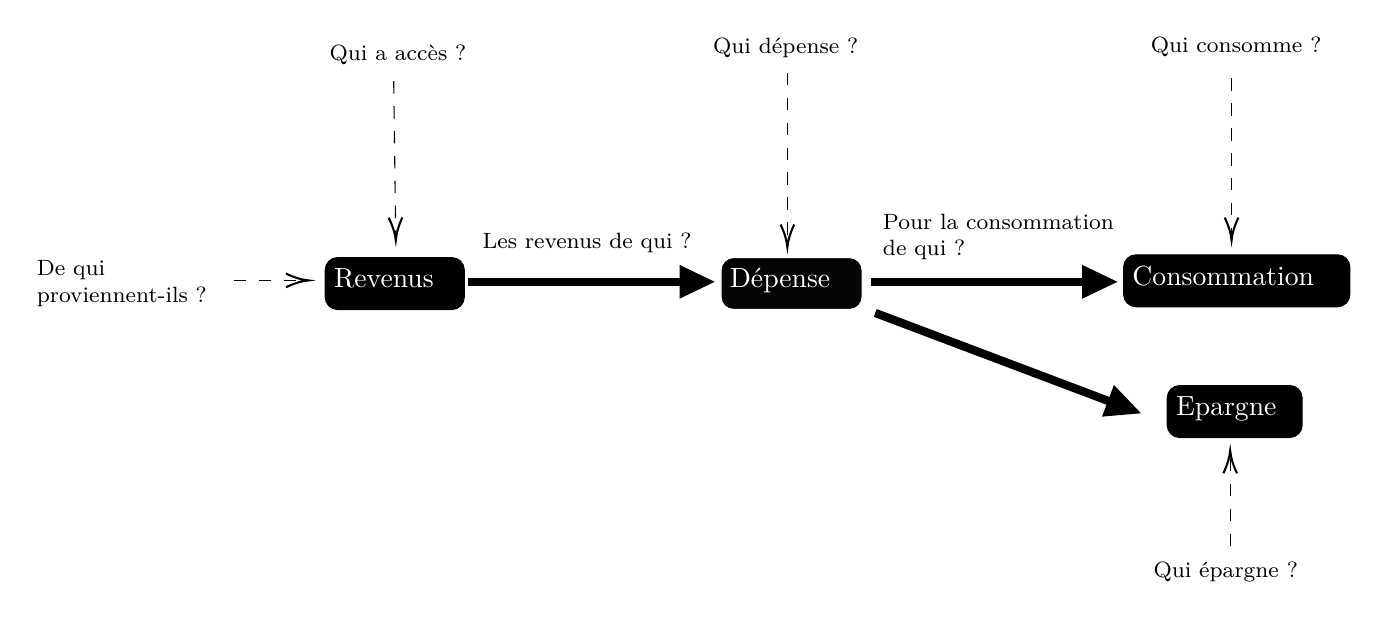
\begin{tikzpicture}[x=0.75pt,y=0.75pt,yscale=-1,xscale=1]
%uncomment if require: \path (0,360); %set diagram left start at 0, and has height of 360

%Straight Lines [id:da591997284273247] 
\draw [line width=3]    (224,187.67) -- (336.67,187.67) ;
\draw [shift={(342.67,187.67)}, rotate = 180] [fill={rgb, 255:red, 0; green, 0; blue, 0 }  ][line width=0.08]  [draw opacity=0] (16.97,-8.15) -- (0,0) -- (16.97,8.15) -- cycle    ;
%Straight Lines [id:da7822778688095842] 
\draw [line width=3]    (418,187.67) -- (530.67,187.67) ;
\draw [shift={(536.67,187.67)}, rotate = 180] [fill={rgb, 255:red, 0; green, 0; blue, 0 }  ][line width=0.08]  [draw opacity=0] (16.97,-8.15) -- (0,0) -- (16.97,8.15) -- cycle    ;
%Straight Lines [id:da7354958436201802] 
\draw  [dash pattern={on 4.5pt off 4.5pt}]  (188,91) -- (188.97,165.67) ;
\draw [shift={(189,167.67)}, rotate = 269.25] [color={rgb, 255:red, 0; green, 0; blue, 0 }  ][line width=0.75]    (10.93,-3.29) .. controls (6.95,-1.4) and (3.31,-0.3) .. (0,0) .. controls (3.31,0.3) and (6.95,1.4) .. (10.93,3.29)   ;
%Straight Lines [id:da6410274435771419] 
\draw  [dash pattern={on 4.5pt off 4.5pt}]  (377.67,87) -- (377.67,169) ;
\draw [shift={(377.67,171)}, rotate = 270] [color={rgb, 255:red, 0; green, 0; blue, 0 }  ][line width=0.75]    (10.93,-3.29) .. controls (6.95,-1.4) and (3.31,-0.3) .. (0,0) .. controls (3.31,0.3) and (6.95,1.4) .. (10.93,3.29)   ;
%Straight Lines [id:da7929911401630845] 
\draw  [dash pattern={on 4.5pt off 4.5pt}]  (591.67,89.67) -- (591.67,165.67) ;
\draw [shift={(591.67,167.67)}, rotate = 270] [color={rgb, 255:red, 0; green, 0; blue, 0 }  ][line width=0.75]    (10.93,-3.29) .. controls (6.95,-1.4) and (3.31,-0.3) .. (0,0) .. controls (3.31,0.3) and (6.95,1.4) .. (10.93,3.29)   ;
%Straight Lines [id:da3206475430119069] 
\draw  [dash pattern={on 4.5pt off 4.5pt}]  (111,187) -- (145,187) ;
\draw [shift={(147,187)}, rotate = 180] [color={rgb, 255:red, 0; green, 0; blue, 0 }  ][line width=0.75]    (10.93,-3.29) .. controls (6.95,-1.4) and (3.31,-0.3) .. (0,0) .. controls (3.31,0.3) and (6.95,1.4) .. (10.93,3.29)   ;
%Straight Lines [id:da9156843538096584] 
\draw [line width=3]    (420,202.67) -- (542.39,248.88) ;
\draw [shift={(548,251)}, rotate = 200.69] [fill={rgb, 255:red, 0; green, 0; blue, 0 }  ][line width=0.08]  [draw opacity=0] (16.97,-8.15) -- (0,0) -- (16.97,8.15) -- cycle    ;
%Straight Lines [id:da028309255882011275] 
\draw  [dash pattern={on 4.5pt off 4.5pt}]  (591,315) -- (591,271) ;
\draw [shift={(591,269)}, rotate = 90] [color={rgb, 255:red, 0; green, 0; blue, 0 }  ][line width=0.75]    (10.93,-3.29) .. controls (6.95,-1.4) and (3.31,-0.3) .. (0,0) .. controls (3.31,0.3) and (6.95,1.4) .. (10.93,3.29)   ;

% Text Node
\draw  [fill={rgb, 255:red, 0; green, 0; blue, 0 }  ,fill opacity=1 ]  (155,182) .. controls (155,178.69) and (157.69,176) .. (161,176) -- (216,176) .. controls (219.31,176) and (222,178.69) .. (222,182) -- (222,195) .. controls (222,198.31) and (219.31,201) .. (216,201) -- (161,201) .. controls (157.69,201) and (155,198.31) .. (155,195) -- cycle  ;
\draw (158,180) node [anchor=north west][inner sep=0.75pt]  [font=\normalsize,color={rgb, 255:red, 255; green, 255; blue, 255 }  ,opacity=1 ] [align=left] {Revenus};
% Text Node
\draw  [color={rgb, 255:red, 255; green, 255; blue, 255 }  ,draw opacity=1 ][fill={rgb, 255:red, 0; green, 0; blue, 0 }  ,fill opacity=0.98 ]  (345.67,182) .. controls (345.67,178.69) and (348.35,176) .. (351.67,176) -- (407.67,176) .. controls (410.98,176) and (413.67,178.69) .. (413.67,182) -- (413.67,195) .. controls (413.67,198.31) and (410.98,201) .. (407.67,201) -- (351.67,201) .. controls (348.35,201) and (345.67,198.31) .. (345.67,195) -- cycle  ;
\draw (348.67,180) node [anchor=north west][inner sep=0.75pt]  [font=\normalsize,color={rgb, 255:red, 255; green, 255; blue, 255 }  ,opacity=1 ] [align=left] {Dépense};
% Text Node
\draw  [fill={rgb, 255:red, 0; green, 0; blue, 0 }  ,fill opacity=1 ]  (539.67,180.67) .. controls (539.67,177.35) and (542.35,174.67) .. (545.67,174.67) -- (642.67,174.67) .. controls (645.98,174.67) and (648.67,177.35) .. (648.67,180.67) -- (648.67,193.67) .. controls (648.67,196.98) and (645.98,199.67) .. (642.67,199.67) -- (545.67,199.67) .. controls (542.35,199.67) and (539.67,196.98) .. (539.67,193.67) -- cycle  ;
\draw (542.67,178.67) node [anchor=north west][inner sep=0.75pt]  [font=\normalsize,color={rgb, 255:red, 255; green, 255; blue, 255 }  ,opacity=1 ] [align=left] {Consommation};
% Text Node
\draw (190.03,78.46) node  [font=\footnotesize] [align=left] {Qui a accès ?};
% Text Node
\draw (379.37,74.8) node  [font=\footnotesize] [align=left] {Qui dépense ? };
% Text Node
\draw (596.37,74.46) node  [font=\footnotesize] [align=left] {Qui consomme ? };
% Text Node
\draw (283.7,169.13) node  [font=\footnotesize] [align=left] {Les revenus de qui ? };
% Text Node
\draw (479.37,166.13) node  [font=\footnotesize] [align=left] {Pour la consommation \\de qui ? };
% Text Node
\draw (57.03,188.46) node  [font=\footnotesize] [align=left] {De qui \\proviennent-ils ?};
% Text Node
\draw (591.37,327.46) node  [font=\footnotesize] [align=left] {Qui épargne ? };
% Text Node
\draw  [fill={rgb, 255:red, 0; green, 0; blue, 0 }  ,fill opacity=1 ]  (560.67,243.67) .. controls (560.67,240.35) and (563.35,237.67) .. (566.67,237.67) -- (619.67,237.67) .. controls (622.98,237.67) and (625.67,240.35) .. (625.67,243.67) -- (625.67,256.67) .. controls (625.67,259.98) and (622.98,262.67) .. (619.67,262.67) -- (566.67,262.67) .. controls (563.35,262.67) and (560.67,259.98) .. (560.67,256.67) -- cycle  ;
\draw (563.67,241.67) node [anchor=north west][inner sep=0.75pt]  [font=\normalsize,color={rgb, 255:red, 255; green, 255; blue, 255 }  ,opacity=1 ] [align=left] {Epargne};


\end{tikzpicture}

\caption{Saisir l'économie domestique}
\end{figure}

L'enquête BDF contient spécifiquement des variables économiques : les
revenus détaillés (revenus d'activité, du patrimoine, de remplacement et
de transferts) sont disponibles à l'échelle individuelle ou à celle du
ménage et parfois aux deux. Certaines dépenses sont renseignées à
l'échelle individuelle et se rapportent à l'individu qui les a effectué
(et renseigné dans son carnet), d'autre sont agrégées ou estimées et
sont donc renseignées à l'échelle du ménage. Le montant consacré à
chaque poste de consommation (détaillé au niveau 5 de la nomenclature)
est n'est disponible qu'au niveau du ménage. De ce fait, le jeu de
données de l'enquête contient plusieurs tableaux pour lesquelles l'unité
d'observation est soit le ménage, soit l'individu. Partant, on ne peux
pas répondre directement à la question de ``Qui dépense l'agent de qui
au bénéficie de qui ?''. Nous avons choisit de questionner le caractère
``commun'' du budget en analysant les liens entre revenus et types de
consommations. On cherche ainsi à saisir le ``marquage social''
(Zelizer, 2005) des revenus au sein des couples en fonction du genre et
du statut parental des membres qui les composent.

\section{Des ``causes communes'' aux périmètres plus
limités}\label{des-causes-communes-aux-puxe9rimuxe8tres-plus-limituxe9s}

On l'a vu, la notion de budget commun, liée à la catégorie statistique
du ``ménage'', est un concept ancré dans la production de la statistique
d'État, plus qu'un concept sociologique. La mise en commun des
ressources, le partage des dépenses et l'équité des consommation ainsi
supposés s'apparentent d'avantage aux \emph{logiques de maisonnées
(Weber, 2002)} qui se déploient dans les groupes familiaux, et qui ne
correspondent pas forcément au contour du ménage. Nous proposons donc de
discuter l'effectivité du budget commun en questionnant les périmètres
des ``causes communes''(Gollac, 2003) dans les familles recomposées par
rapport aux autres couples avec enfants. Les ``causes communes''
mobilisent l'ensemble de la maisonnée dans un processus de coopération
productive. Elles sont, par exemple, la préservation d'une maison ou
d'une entreprise familiale, ou la prise en charge de personnes
dépendantes. En ce sens, élever des enfants constituent sans doute la
``cause commune'' la plus ordinaire de toute, et qui justifie alors la
mise en commun partielle de ressources (Roy, 2005). Les logiques de
maisonnée, centrées autour de ``cause commune'', s'articulent alors avec
des logiques de lignées. \textbf{En d'autres termes, on peut ici
considérée qu'une large mise en commun des ressources, un partage des
dépenses et une équité de consommation dans les familles recomposée,
notamment de celles déstinées constituraient un}

\subsection{Dépenses féminines et dépenses
masculines}\label{duxe9penses-fuxe9minines-et-duxe9penses-masculines}

Faute de pouvoir saisir directement l'appartenance de l'argent qui est
dépensé dans différents types de consommations, nous en avons chercher
des traces dans l'enquête. Nous avons ainsi choisi de modéliser
l'utilisation de l'argent féminin et de l'argent masculin dans les
ménages formés par des couples ayant des enfants à charge. Pour cela
nous avons réalisé des régressions sur les différents types de
consommations selon les méthodes classiques employés par les travaux sur
le sujet (Phipps et Burton, 1998~; Roy, 2006). Il s'agit de modéliser la
sensibilité de différents types de consommation à l'augmentation des
revenus féminin et masculins. Pour chaque type de consommation, agrégé
au niveau 2 de la nomenclature, nous effectuons donc une régression
linéaire censurée\footnote{Il s'agit d'un modèle de régression de Tobit,
  adapté aux variables continues pour lesquelles la valeur 0 est
  sur-représentée et dont la distribution suit une courbe de Gauss} sur
le montant qui y est consacré dans laquelle nous introduisons deux
termes d'interaction : entre le revenu féminin et le type de
configuration familiale d'une part et entre le revenu masculin et le
type de configuration d'autre part. Afin de contrôler les différentes
différents facteurs influençant la consommation de différents types de
biens et de services, nous introduisons dans le modèle la variable
codant l'appartenance à des fraction de classe {[}Voir chapitre 2{]} qui
résume de manière synthétique à la fois les positions professionnelles
des conjoints, leur niveau de diplôme, l'âge des conjoints, le niveau de
vie du ménage, leur niveau de vie, que le nombre d'enfants dans le
ménage. Nous avons ici préféré introduire une variable synthétique de la
position sociale au niveau du ménage plutôt qu'un nombre plus important
de variables au niveau individuel compte tenu des effectifs relativement
faibles dont nous disposons.

\begin{encadre}{Equation du modèle}

$$
M_k = \alpha + \beta_1 Y_F*T + \beta_2 Y_H*T + \beta_3 T + \beta_4 Y_M + \beta_5 C + \beta_6 N + \beta_7 L + \epsilon
$$
avec : 

- $M_k$, le montant dépensé par le ménage pour la consommation de $k$

- $Y_F$, les revenus féminin, 

- $Y_M$, les revenus masculins

- $Y_M$, le revenu disponible du ménage

- $T$, le type de configuration familiale du méange (traditionelle vs recomposée)

- $C$, la position sociale du ménage synthétique

- $N$, le nombre d'enfants du ménage

- $L$, le statut d'occupation du logement (propriétaire, locataire, autre)

\end{encadre}

Ainsi on peut, à position sociale, nombre d'enfants et statut
d'occupation du logement du ménage égaux, comparer l'effet de
augmentation du revenu féminin ou masculin sur les dépenses effectuées
par le ménage. On effectue un test de Wald sur les coefficients
respectifs des revenus masculin et féminin dans les familles
traditionnelles et recomposées pour identifier les différences
statistiquement significatives.

Une différence significative ne signifie pas pour autant que l'argent
des femmes ou respectivement des hommes est utilisé pour les dépenses
auxquelles elles sont corrélés et consommé par celui ou celle dont
provient l'argent. Cela signifie simplement que l'augmentation du revenu
masculin ou féminin a des effets sur le montant dépensé par le ménage
sur ces différents postes. On ne peut pas par exemple exclure que
l'augmentation du revenu féminin dans couple conduisent les couples à
modifier l'arrangement économique en lien avec le loyer, par exemple en
passant d'un 55\%-45\% à un 50\%-50\%, ce qui libereait l'argent
masculin qui pourrait être consacré à d'autres dépenses, par exemple en
loisir. Ainsi, dans le modèle, l'augmentation du revenu féminin se
traduirait par une augmentation des consommations de loisir du ménage,
sans pour autant que ce loisir ait été consommé par la femme. Pour
autant, la sensibilité des consommations au revenu des hommes et des
femmes constitue un bon moyen d'approcher la mise en commun des
ressources et le partage des dépenses (Roy, 2006). L'autre problème de
l'utilisation de cette méthode est la linéarisation de l'effet de
l'augmentation de revenu. Nous avons cherché à limiter ce problème en
utilisant un modèle de tobit plutôt qu'un OLS classique, ce qui permet
une meilleur prise en compte de la sur-représentation des valeurs nulles
sur certaines dépenses. Cependant, 100 euros de plus n'ont pas
nécessairement les mêmes effets lorsqu'on gagne 600 euros par mois que
lorsque en gagne 3 000. Le tableau ci-dessous présente les résultats de
ces régressions de Tobit sur la consommation totale annuelle du ménage.

\begin{table}[!h]
\centering\centering
\caption{Regression sur le montant de consommation et d'épargne annuel}
\centering
\fontsize{8}{10}\selectfont
\fontsize{7}{9}\selectfont
\begin{threeparttable}
\begin{tabular}[t]{lcccc}
\toprule
\multicolumn{1}{c}{ } & \multicolumn{2}{c}{\textbf{Table 1}} & \multicolumn{2}{c}{\textbf{Table 2}} \\
\cmidrule(l{3pt}r{3pt}){2-3} \cmidrule(l{3pt}r{3pt}){4-5}
\textbf{Caractéristique} & \textbf{Beta} & \textbf{95\% IC} & \textbf{Beta} & \textbf{95\% IC}\\
\midrule
<span style=" font-weight: bold;    " >Fraction de classe</span> &  &  &  & \\
\hspace{1em}Classes moyennes superieures [C4] & — & — & — & —\\
\hspace{1em}Classes populaires précaires [C3] & -14 000*** & -16 492 – -11 508 & 14 569*** & 10 980 – 18 158\\
\hspace{1em}Classes populaires célibataires et urbaines [C6] & -5 935*** & -8 068 – -3 801 & 4 794** & 1 710 – 7 879\\
\hspace{1em}Petits indépendants [C5] & -2 282* & -4 515 – -49 & -1 379 & -4 663 – 1 905\\
\addlinespace
\hspace{1em}Petits-moyens [C1] & -4 913*** & -6 467 – -3 358 & 5 938*** & 3 727 – 8 150\\
\hspace{1em}Bourgeoisie culturelle [C2] & -793 & -3 055 – 1 468 & 43 & -3 183 – 3 268\\
\hspace{1em}Bourgeoisie économique [C7] & 7 390*** & 5 299 – 9 481 & -8 352*** & -11 299 – -5 404\\
<span style=" font-weight: bold;    " >Statut d'occupation du logement</span> &  &  &  & \\
\hspace{1em}Propriétaire & — & — & — & —\\
\addlinespace
\hspace{1em}Autre & -704 & -4 801 – 3 393 & 272 & -5 639 – 6 182\\
\hspace{1em}Locataire & 4 778*** & 3 188 – 6 367 & -6 717*** & -9 015 – -4 419\\
<span style=" font-weight: bold;    " >Nombre d'enfants dans le ménage</span> & 2 360*** & 1 753 – 2 967 & 1 578*** & 705 – 2 451\\
<span style=" font-weight: bold;    " >Configuration familiale</span> &  &  &  & \\
\hspace{1em}Traditionelle & — & — & — & —\\
\addlinespace
\hspace{1em}Recomposée & 672 & -2 379 – 3 724 & -1 769 & -6 191 – 2 653\\
<span style=" font-weight: bold;    " >Revenu féminin * Configuration familiale</span> &  &  &  & \\
\hspace{1em}Revenu féminin * Traditionelle & 36*** & 32 – 40 & 50*** & 44 – 56\\
\hspace{1em}Revenu féminin * Recomposée & 43*** & 30 – 56 & 52*** & 34 – 71\\
<span style=" font-weight: bold;    " >Configuration familiale * Revenu masculin</span> &  &  &  & \\
\addlinespace
\hspace{1em}Traditionelle * Revenu masculin & 23*** & 21 – 25 & 56*** & 53 – 59\\
\hspace{1em}Recomposée * Revenu masculin & 21*** & 14 – 28 & 53*** & 43 – 63\\
\bottomrule
\multicolumn{5}{l}{\rule{0pt}{1em}\textsuperscript{1} \textit{p<0.05; \textbf{p<0.01; }}p<0.001}\\
\multicolumn{5}{l}{\rule{0pt}{1em}\textsuperscript{2} IC = intervalle de confiance}\\
\end{tabular}
\begin{tablenotes}
\item \textit{Note: } 
\item Source : Budget de famille, 2017
\item Champ : ménages formées par des couples dont au moins l'un des membres est un adulte agé de 25 à 56 ans et vivant avec au moins un enfant de moins de 25 ans (N = 4287).
\item Lecture : Toutes choses égales par ailleurs, les locatiares dépensent en moyenne 4 778 euros de plus par ans que les propriétaires. 
\end{tablenotes}
\end{threeparttable}
\end{table}

Il montre que, toutes choses égales part ailleurs, la consommation
dépend de l'appartenance de classe du ménage : plus les ménages qui font
parties des fractions favorisées, plus leurs dépenses de consommations
annuelles sont élevés. Le fait d'être locataire de son logement conduit
également à dépenser d'avantage au cours de l'année, ce qui s'explique
facilement par le poids des loyers dans le budget. Enfin le nombre
d'enfants a aussi un fort effet sur les dépenses du ménage, puisqu'un
enfant supplémentaire conduit, en moyenne, à dépenser 2 360 euros
supplémentaire par ans. Enfin, on observe que la consommation totale
annuelle est plus sensible aux revenus féminins qu'au revenus masculins.
Ainsi, toutes choses égales part ailleurs, une augmentation de 100 euros
du revenu féminin dans un ménage à la configuration familiale
traditionnelle, se traduit par une augmentation de 36 euros de la
consommation annuelle, contre 23 euros pour les hommes vivants dans ces
familles. On obsreve la même chose dans les familles recomposées. D'une
manière générale, on ne peut pas analyser de manière symétrique
l'influence de l'augmentation des revenus féminins et des revenus
masculins. Ces revenus sont marqués socialement, et ne signifient pas la
même chose suivant qu'ils proviennent du travail féminin ou du travail
masculin. Ainsi, les revenus masculins ont longtemps été considéré comme
les revenus principaux d'un ménage, supposés pouvoir seuls pourvoir aux
besoins du groupe familial. A l'inverse les revenus féminins sont
considérés comme des revenus d'appoints, complémentaires aux revenus
masculins et donc utilisés pour améliorer l'ordinaire. Cela explique
pourquoi lorsque les dépenses sont différemment sensibles aux revenus
des hommes et des femmes, elles sont en général, plus sensibles aux
revenus féminins qu'aux revenus masculin. Cela est d'autant plus vrai
pour les postes de dépenses dont part dans le budget augmente avec le
niveau de vie : les transports, les loisirs et la culture, les
restaurants et hôtels ainsi que les biens et services divers. C'est
aussi le cas du logement qui représente une part importante des budgets
des ménages pauvres et plus faible pour les ménages aisées, mais dont le
montant des dépenses augmente rapidement avec le revenu.

\subsection{Des dépenses moins partagées entre hommes et femmes que dans
les familles
traditionnelles}\label{des-duxe9penses-moins-partaguxe9es-entre-hommes-et-femmes-que-dans-les-familles-traditionnelles}

Cependant, les résultats précédants montrent également que dans les
ménages à la configuration familiale recomposée, l'écart de sensibilité
de la consommation entre les revenus féminins et les revenus masculins
est plus important que dans les familles traditionnelles. Une
augmentation de 100 du revenu féminin se traduit, en moyenne, par une
augmentation de la consommation annuelle de 43 euros, contre 21 euros
pour une augmentation du revenu masculin. Si la sensibilité de la
consommation annuelle aux revenus masculins n'est pas significativement
différente dans les ménages à la configuration familiales recomposée et
traditionnelle, ce n'est pas le cas pour les revenus féminins : ils font
d'avantage augmenter la consommation dans les familles recomposées que
dans les familles traditionnelles.

Dans les familles recomposées, certains de postes budgétaires sont en
effet significativement plus sensibles à l'augmentation des revenus
féminins que dans les familles traditionnelles.

\begin{figure}[H]

{\centering \includegraphics[width=1\linewidth]{Memoire_files/figure-latex/ggcoef-1} 

}

\caption{Sensibilité des différents types de consommation aux revenus féminins et masculin dans les familles traditionelles et recomposées}\label{fig:ggcoef}
\end{figure}

Il y a d'abord les postes de dépenses qui apparaissent aussi sensibles
aux revenus de l'homme qu'aux revenus de la femme dans les familles
traditionnelles comme dans les familles recomposées. C'est le cas de la
santé pour laquelle la différence de sensibilité n'est pas significative
entre les revenus féminins et masculins dans le premier cas comme dans
le second. C'est également le cas pour les dépenses d'enseignements et
les dépenses de communication. Pour ces dépenses, il s'agit
principalement de tarifs forfaitaires : prix d'une consultation chez un
médecin, coût d'un abonnement téléphonique, tarif de l'étude après
l'école. Ces dépenses sont d'une manière générale peu sensibleS aux
revenus. Elles représentent certes une part assez faible du budget des
ménages (chiffres issues du tableau structure budgétaire) mais leur
montant n'augmente que très peu avec l'augmentation du revenu (en
particulier pour la santé et les communications). On a donc ici à faire
à des dépenses probablement assez fixes. Il en va de même pour les
dépenses pour les dépenses d'alcool, de tabac et de stupéfiant, qui, du
fait du pouvoir addictif, peuvent également s'apparenter à des dépenses
fixes.

Ensuite, certains postes budgétaires plus sensibles aux revenus féminins
que masculins dans les familles traditionels appairessent encore plus
sensibles dans les familles recomposées. C'est le cas pour le logement,
les restaurants et hôtels, les loisirs et la culture ainsi que les biens
et services divers. Ainsi, ces dépenses apparaissent comme des dépenses
féminines dans l'ensemble des ménages formés par des couples vivants
avec des enfants, mais plus fortement dans les ménages recomposées.
Elles sont donc probablement moins partagées dans les familles
recomposées que dans les familles traditionnelles. D'autres dépenses ne
sont pas significativement sensibles aux revenus féminins ou masculins
dans les familles traditionnelles mais le sont dans les familles
recomposées. C'est le cas des dépenses d'habillement, qui semblent ainsi
faire partie du champ des dépenses communes dans les familles
traditionnelles : un euro supplémentaire gagné par un homme a le même
effet sur ces dépenses qu'un euros supplémentaire gagné par une femme. A
l'inverse, dans les familles recomposées, cents euros supplémentaire
gagné par une femme fait augmenter de 3 euros le budget annuel consacré
aux vêtements, alors que les revenus masculins n'ont pas d'influence
significative sur les dépenses de vêtement et chaussures. Il semble donc
que le partage des dépenses d'habillement ne soit pas fréquente dans les
familles recomposée. Ces postes de dépenses étant, en partie au moins,
des consommations individuelles, on peut penser que ce qui joue ici est
lié au statut de parent ou de beau-parent. Ainsi, il semble que les
charges que représentent les vêtements et chaussures soient portées par
les femmes, plus probablement les mères dans les familles recomposées.

D'autres dépenses sont significativement sensibles aux revenus féminins
par rapports aux revenus masculins dans les familles traditionnelles,
mais cette différence n'est pas significative dans les familles
recomposées : il s'agit des dépenses en matière d'alimentation et de
transport, qui représentent deux des plus gros postes des dépenses des
ménages, mais aussi de meubles et d'entretien courant du logement. Cela
semble s'expliquer par la variance très importante des coefficients
estimés pour les revenus masculins et surtout féminins pour ces dépenses
dans familles recomposées. Les effectifs de ménages dont la
configuration familiale est recomposée sont en effet bien plus faibles
que ceux des familles traditionnelles, il est donc normal que les
intervalles de confiances des coefficients estimés par les modèles
soient plus étendus. Cependant, cela pourrait aussi s'expliquer par des
pratiques différentes des hommes et des femmes en fonction de leur
statut de parent ou de beau-parent.

\subsection{Beux-pères et belles-mères : des contributions
assymétriques}\label{beux-puxe8res-et-belles-muxe8res-des-contributions-assymuxe9triques}

Pour essayer de comprendre à quoi sont dues ces variations de
sensibilité des différents types de consommation aux revenus féminins et
masculins dans les familles recomposées, nous avons procédé à une
modélisation similaire sur la sous-population des ménages aux
configurations familiales recomposées. Cependant fois-ci au lieu des
interactions précédentes nous introduisons deux autres interactions,
d'une part une entre les revenus féminins et l'existence d'enfants de la
femme dans le ménage et d'autre part les revenus masculins et
l'existence d'enfants de l'homme dans le ménage. Les coefficient ainsi
estimés traduisent donc l'effet du revenu des mères, des pères, des
beaux-pères sans enfants et des belles-mères sans enfants sur différents
postes de dépenses. Il s'agit ici de saisir les conditions de
possibilité de la participations économique des pères, des beaux-pères,
des mères et des belles-mères aux différentes ``charges du ménage''.

\begin{figure}[H]

{\centering \includegraphics[width=1\linewidth]{Memoire_files/figure-latex/regFamRecompConso-1} 

}

\caption{Sensibilité des différents postes de dépenses aux revenus féminins et masculin en fonction de la situation parentale dans les familles recomposées}\label{fig:regFamRecompConso}
\end{figure}

Comme on pouvait s'y attendre, les postes des dépenses aussi sensibles
aux revenus masculins et qu'aux revenus féminins dans les familles
recomposées ne présentent pas de différences significatives suivant le
statut parental. En ce qui concerne l'alimentation, la santé, le tabac,
l'alcool et les stupéfiants, l'enseignement, l'argent des pères, des
mères, des belles-mères et des beaux-pères sans enfants a un effet
similaire sur les dépenses. D'autres postes de dépenses sont marqués par
le genre de l'individu dont provient le revenu, mais assez peu par son
statut parental. C'est le cas des dépenses en matière de vêtements et de
chaussures et de biens et de restauration et hôtel, ainsi que de meuble
et d'entretien de la maison, qui sont avant tout des dépenses liées aux
revenus féminins, et assez peu au revenu masculin dans les familles
recomposées. Ces dépenses reflettent à la fois les consommations les
plus féminines (vêtements, entretien de la maison), et celles qui
permettent de ``se faire plaisir'' (\textbf{cartieramossé?})
(restaurant, vêtements).

Tous les autres postes budgétaires sont à la fois sensibles au genre et
au statut parental de l'individu dont proviennent les revenus. Par
exemple, la consommation en loisir et culture est surdéterminée par le
revenu des mères, et celle en communication par le revenus des
belles-mères sans enfants. En ce qui concerne le logement on observe un
effet intéressant. Dans les familles recomposées, les revenus féminins
paraissaient déterminer plus fortement que les revenus masculins les
dépenses en matière de logement. Cependant, on voit qu'en différenciant
ceux-ci en fonction du statut parental, on observe une
sous-détermination des dépenses de logement par les revenus des
beaux-pères sans enfants, là où les coefficients ne sont pas
significativement différents pour les belles-mères sans enfants, les
mères et les pères. Plusieurs hypothèses peuvent expliquer cela. D'une
part, les recompositions familiale peuvent donner lieu à emménagement
d'un des conjoint-e-s, plus probablement celui ou celle qui n'a pas
d'enfants, au domicile de l'autre, sans que cela ne donne lieu a un
partage des charges liées au logement. Cependant, on devrait donc
observer le même effet pour les belles-mères. Or ce n'est pas le cas.
Ceci semble indiquer que les revenus des belles-mères déterminent tout
autant les dépenses en matière de logement que celles des pères, là ou
dans les couples constituée d'une femme ayant des enfants et d'un homme
n'en ayant pas, seuls les revenus de cette dernière détermine les
dépenses en matière de logement.

Pour les biens et service divers, les revenus des pères ont plus d'effet
que les revenus des beaux-pères et les revenus des mères on plus d'effet
que les revenus des belles mères. Il semble donc la consommation en
biens et services divers soit liée au fait d'avoir des enfants. Les
biens et services divers contiennent en effet les services de garde
d'enfant qui peuvent représenter un poste de consommation
non-négligeable, et qui expliquerait que les revenus des parents soit
sur-déterminants dans ce type de dépenses. En revanche, ce sont bien les
revenus des mères qui déterminent le plus fortement ce type de
consommation. Cela rejoint les analyses selon lesquelles les services
payants permettant de réduire le travail domestique effectué
gratuitement par les femmes dans les familles est un ``bien supérieur
féminin''. En l'occurrence, la garde d'enfant, si elle est une affaire
de parent, reste surtout une affaire de mères. On peut ainsi penser que
si les pères de famille recomposée y ont plus recours que les
beaux-pères, ils peuvent néanmoins compter sur leur conjointe, même
lorsque celle-ci n'as pas d'enfants, pour effectuer une partie du
travail domestique et parental. Il est en revanche moins probable que
les mères de familles recomposées puissent faire reposer une partie de
ce travail sur leur conjoint, en particulier lorsque celui-ci n'as pas
lui-même d'enfant.

Ainsi, les revenus féminins déterminent d'avantage le budget consacré
aux postes de consommations genrés dans les couples formés par une mère
et un beau père sans enfant que dans ceux formés par un père et une
belle-mère sans enfants, alors même que les premiers sont en moyenne
moins inégalitaires que les seconds.

Ainsi dans les ménages à la configuration familiale recomposée, on
observe une plus forte séparations des budgets entre homme et femme que
dans les familles traditionnelles, qui est liée, aux statut parentaux
asymétriques qu'ils occupent dans ces familles. Sans la ``cause
commune'' que représente les enfants communs au couple, les
beaux-parents sans enfants, et en particulier les beaux-pères semblent
moins contribuer que les pères à certains postes budgétaires. Ces
résultats tendent à confirmer ceux qui ressortent des entretiens
réalisés avec des parents d'enfants en résidence alternée par
(\textbf{brunet2008?}) qui décrivent plutôt des beau-parents,
majoritairement des beau-pères, peu engagés financièrement, en dehors de
l'alimentation, dans l'entretien des enfants de leur conjoint-e. Les
autrices de l'enquête explique cette absence de contribution par le rôle
que la résidence alternée confère à l'autre parent et qui ne laisserait
pas de ``place'' aux beaux-parents. Pourtant, même en cas de résidence
principale fixée chez un seul des parents, le maintien des liens avec le
parent non gardien reste plutôt fréquent puisqu'en 2005 seuls 13\% des
enfants mineurs qui vivaient sans leur père ne le voyaient jamais
(\textbf{reigner2013?}).

\section{Des mères et des belles-mères au travail
domestique}\label{des-muxe8res-et-des-belles-muxe8res-au-travail-domestique}

Ainsi, si les beaux-parents contribuent financièrement moins à
l'entretien des enfants de leur conjoint-e que ne le feraient des
parents, cela ne signifie pas pour autant qu'aucune forme de parenté
pratique ne se construit entre beaux-parents et beaux-enfants. La notion
de parenté pratique, telle que définie par Florence Weber, dépasse
largement les simples transferts financiers pour englober une variété de
pratiques sociales, économiques et affectives qui structurent la vie
quotidienne des familles. Florence (Weber, 2013) souligne que la parenté
pratique se manifeste par des échanges de services, des soutiens
émotionnels et des interactions quotidiennes qui cimentent les relations
familiales. Par exemple, les soins apportés aux enfants,
l'accompagnement des personnes âgées, l'aide apportée lors d'évènements
importants de la vie ou même les simples actes de solidarité entre
membres de la famille sont autant de manifestations de la parenté
pratique. En ce sens, la dimension matérielle de la parenté ne peut être
réduite à de simple transferts financiers. Ainsi, les arrangements
économiques au sein des familles ne doivent pas être envisagé comme
purement monétaires. Comme le souligne (\textbf{Bessières?}), ces
arrangements englobent un ensemble de pratiques et de contributions qui
vont bien au-delà des simples transferts financiers. Ils incluent
notamment les tâches ménagères, les soins aux enfants, les services
rendu entre membre de la famille, tels que la garde d'enfants ou l'aide
aux travaux ménagers.

\begin{encadre}{Le travail domestique et parental dans l'enquête Budget de famille 2017}

Dans l'enquête Budget de famille (2017), un module portant sur les
activités domestique est prévu. L'individu répondant aux question de
l'enquêteur ou l'enquêtrice est interrogé sur la participation des
différents membres du ménage au travail domestique et parental la
semaine précédant l'entretient. La période d’observation est donc la
même que celles des dépenses. Les variables issues de ces réponses sont
ainsi renseignées dans la table de données sur les dépenses
individuelles. En revanche ce module de question n'est posé qu'à la
moitié des ménages, sélectionnes au hasard, réduisant ainsi la taille de
l’échantillon sur lequel nous travaillons dans cette partie. De plus,
pour une raison que nous ignorons et qui n'est pas explicitée dans la
documentation de l'enquête, parmi les ménages ayant des enfants
cohabitant, les items relatifs au travail parental (aide scolaire aux
enfants et habillage des enfants) ont un nombre très élevé de valeurs
manquantes. Ceci explique pourquoi les p-valeurs calculées sur les tests
du $Chi^2$ sont en général plus élevées. Enfin les questions portent sur
le fait d'avoir effectuer ou non certaines taches et non sur le volume
horaires consacré à ces taches. Une mesure précise de la répartition du
temps de travail domestique n'est donc pas possible.

\end{encadre}

\subsection{Un partage des taches domestiques et parentales entre homme
et femme plus
équitable}\label{un-partage-des-taches-domestiques-et-parentales-entre-homme-et-femme-plus-uxe9quitable}

Le tableau ci-dessous présente le taux de participation des hommes et
des femmes au travail domestique et parental la semaine ayant précédé
l'entretien. Il distinguent différentes activités domestiques en
déclinant différentes taches.

\begin{table}[!h]
\centering\centering
\caption{\label{tab:unnamed-chunk-19}Implication dans le travail domestique et parental en fonction de la configuration familiale et du sexe}
\centering
\fontsize{8}{10}\selectfont
\resizebox{\ifdim\width>\linewidth\linewidth\else\width\fi}{!}{
\fontsize{7}{9}\selectfont
\begin{threeparttable}
\begin{tabular}[t]{lccccccccc}
\toprule
\multicolumn{1}{c}{ } & \multicolumn{4}{c}{\makecell[c]{\textbf{Homme}\\(46\%)}} & \multicolumn{4}{c}{\makecell[c]{\textbf{Femme}\\(54\%)}} & \multicolumn{1}{c}{ } \\
\cmidrule(l{3pt}r{3pt}){2-5} \cmidrule(l{3pt}r{3pt}){6-9}
 & \makecell[c]{\textbf{Traditionelle}\\(84\%)} & \makecell[c]{\textbf{Recomposée}\\(11\%)} & \makecell[c]{\textbf{Monoparentale}\\(5,1\%)} & \textbf{p-valeur} & \makecell[c]{\textbf{Traditionelle}\\(72\%)} & \makecell[c]{\textbf{Recomposée}\\(9,3\%)} & \makecell[c]{\textbf{Monoparentale}\\(18\%)} & \textbf{p-valeur} & \textbf{Ensemble}\\
\midrule
\addlinespace[0.3em]
\multicolumn{10}{l}{\textbf{Activité effectuée la semaine de l'enquête (en \%)}}\\
\hspace{1em}\textbf{Aide scolaire aux enfants, } & 26 & 24 & 22 & 0,9 & 36 & 33 & 25 & 0,068 & 30\\
\hspace{1em}\textbf{Bricolage, } & 47 & 44 & 33 & 0,060 & 10 & 12 & 15 & 0,028 & 27\\
\hspace{1em}\textbf{Habillage des enfants, } & 72 & 70 & 100 & 0,065 & 89 & 90 & 84 & 0,2 & 81\\
\hspace{1em}\textbf{Courses, } & 63 & 70 & 88 & <0,001 & 88 & 89 & 93 & 0,014 & 78\\
\hspace{1em}\textbf{Cuisine du quotidien, } & 55 & 56 & 95 & <0,001 & 93 & 91 & 96 & 0,049 & 77\\
\hspace{1em}\textbf{Cuisine de récéption, } & 11 & 8,9 & 18 & 0,073 & 22 & 23 & 14 & <0,001 & 16\\
\hspace{1em}\textbf{Menage, } & 44 & 54 & 88 & <0,001 & 90 & 90 & 95 & 0,040 & 71\\
\hspace{1em}\textbf{Jardinage, } & 31 & 26 & 22 & 0,2 & 19 & 15 & 14 & 0,069 & 23\\
\hspace{1em}\textbf{Repassage, } & 9,7 & 13 & 26 & <0,001 & 57 & 49 & 54 & 0,11 & 35\\
\hspace{1em}\textbf{Vaisselle, } & 52 & 53 & 75 & 0,001 & 82 & 78 & 89 & 0,006 & 69\\
\textbf{Effectifs, (non-pondérés)} & 1673 & 253 & 124 &  & 1673 & 263 & 876 &  & 4862\\
\bottomrule
\multicolumn{10}{l}{\rule{0pt}{1em}\textsuperscript{1} Pearson's X\textasciicircum{}2: Rao \& Scott adjustment}\\
\end{tabular}
\begin{tablenotes}
\item \textit{Note: } 
\item Source : Budget de famille, 2017
\item Champ : Individus adultes agés de 25 à 65 ans ou en couple avec un adulte agé de 25 à 65 ans, formant des ménages ordinaires avec au moins un enfant. (N = ).
\item Lecture : 47\% des hommes vivants en famille traditionelle ont fait du bricolage la semaine de l'enquête.
\end{tablenotes}
\end{threeparttable}}
\end{table}

En ce qui concerne la plus part des taches domestique et parentales, les
femmes vivants en familles traditionnelles et recomposées apparaissent
impliquées dans des proportions similaires. Le variations significatives
d'implications des femmes dans le travail domestique et parental
tiennent en général à la situation de monoparentalité par rapport à la
vie en couple. Les femmes vivant en famille recomposée apparaissent
cependant légèrement mais significativement moins impliquées dans le
repassage (elles sont seulement 49\% a avoir repasser des vêtements la
semaine de l'enquête contre 57\% des femmes vivant en famille
traditionnelle et 54\% des femmes vivants en famille recomposée). En
revanche les hommes vivants en familles recomposées apparaissent plus
impliqués dans certaines tâches que ceux vivants en famille
traditionnelles. Ils sont en effet plus nombreux à avoir fait du
repassage (13\% contre 9,4\%), des courses (70\% contre 63\%) ou du
ménage (54\% contre 44\%). La participation féminine sur ces taches ne
diffère pas significativement entre familles recomposées et familles
traditionnelles. Il semblent donc que les couples formant des ménages
recomposées soient plus égalitaires : les hommes y sont légèrement plus
engagé dans la prise en charge du travail domestique. Ces résultats
confirmes ceux obsrevés par Domingo (2009) et Solaz (2021) à partir de
l'enquête Etudes des relations familiales e intergénérationelles (ERFI).
On peut se demander si l'effet observé n'est pas lié au statut parental.
D'une part, la mobilisation légèrement plus forte des hommes sur le
travail domestique pourrait être liée aux pères qui ont des enfants
issus d'une précédente union et qui, ayant probablement connu une
période de monoparentalité avant leur remise en couple ont du assurer
eux même, au moins en partie, le travail domestique et parental lié au
fait d'élever seul ses enfants. D'autre part, les belles-mères sans
enfants sont largement sous-représentées parmi les femmes vivant en
famille recomposées, on ne peut donc pas exclure qu'elles soient moins
mobilisées que les mères. Le tableau ci-dessous présente la part de
parents vivants en avec au moins un de leurs enfant ayant effectué des
taches de travail domestique et parentales durant la semaine de
l'enquête.

\begingroup\fontsize{7}{9}\selectfont
\begingroup\fontsize{8}{10}\selectfont

\begin{ThreePartTable}
\begin{TableNotes}
\item \textit{Note: } 
\item Source : Budget de famille, 2017
\item Champ : Parents agés de 25 à 65 ans ou en couple avec un adulte agé de 25 à 65 ans, formant des ménages ordinaires et vivant avec au moins un de leurs enfants (N = ).
\item Lecture : 76\% des parents vivants en famille traditionelle ont fait les courses au moins une fois durant la semaine de l'enquête.
\end{TableNotes}
\begin{longtable}[t]{>{\raggedright\arraybackslash}p{3cm}cccccc}
\caption{\label{tab:unnamed-chunk-20}Travail domestique et parental des parents en fonction de la configuration familiale}\\
\toprule
 & \makecell[c]{\textbf{Traditionelle}\\(78\%)} & \makecell[c]{\textbf{Recomposée}\\(7,5\%)} & \makecell[c]{\textbf{Monoparentale}\\(12\%)} & \makecell[c]{\textbf{Autre}\\(2,1\%)} & \textbf{Ensemble} & \textbf{p-valeur}\\
\midrule
\endfirsthead
\caption[]{Travail domestique et parental des parents en fonction de la configuration familiale \textit{(continued)}}\\
\toprule
 & \makecell[c]{\textbf{Traditionelle}\\(78\%)} & \makecell[c]{\textbf{Recomposée}\\(7,5\%)} & \makecell[c]{\textbf{Monoparentale}\\(12\%)} & \makecell[c]{\textbf{Autre}\\(2,1\%)} & \textbf{Ensemble} & \textbf{p-valeur}\\
\midrule
\endhead

\endfoot
\bottomrule
\insertTableNotes
\endlastfoot
\addlinespace[0.3em]
\multicolumn{7}{l}{\textbf{Activité effectuée la semaine de l'enquête (en \%)}}\\
\hspace{1em}\textbf{Aide scolaire aux enfants,  \%} & 31 & 31 & 25 & 31 & 30 & 0,6\\
\hspace{1em}\textbf{Bricolage,  \%} & 29 & 27 & 19 & 21 & 27 & <0,001\\
\hspace{1em}\textbf{Habillage des enfants,  \%} & 80 & 83 & 86 & 68 & 81 & 0,070\\
\hspace{1em}\textbf{Courses,  \%} & 76 & 83 & 92 & 77 & 78 & <0,001\\
\hspace{1em}\textbf{Cuisine du quotidien,  \%} & 74 & 76 & 96 & 81 & 77 & <0,001\\
\hspace{1em}\textbf{Cuisine de récéption,  \%} & 16 & 16 & 15 & 8,1 & 16 & 0,3\\
\hspace{1em}\textbf{Menage,  \%} & 67 & 74 & 93 & 79 & 71 & <0,001\\
\hspace{1em}\textbf{Jardinage,  \%} & 25 & 22 & 16 & 12 & 23 & <0,001\\
\hspace{1em}\textbf{Repassage,  \%} & 33 & 33 & 48 & 54 & 36 & <0,001\\
\hspace{1em}\textbf{Vaisselle,  \%} & 67 & 67 & 86 & 74 & 70 & <0,001\\
\textbf{Effectifs, (non-pondérés)} & 3346 & 385 & 1000 & 174 & 4905 & \\*
\multicolumn{7}{l}{\rule{0pt}{1em}\textsuperscript{1} Pearson's X\textasciicircum{}2: Rao \& Scott adjustment}\\
\end{longtable}
\end{ThreePartTable}
\endgroup{}
\endgroup{}

Pour la majorité des taches, la proportion de parent vivant en famille
recomposée ayant effectué cette tache au moins une fois au cours de la
semaine de l'enquête apparaît similaire à celle des parents vivants en
familles traditionnelle, alors qu'elle apparaît plus importante dans les
familles monoparentales. Cela tend à faire penser que la remise en
couple cohabitant permet, pour les parents célibataires, de partager
avec une autre personne une partie au moins des taches domestiques.
Cependant, ils sont significativement (p \textless{} 0,001) plus
nombreux avoir fait les courses et le ménage au moins une fois la
semaine de l'enquête : 83\% ont fait les courses contre 76\% dans les
familles traditionnelles et 74\% on fait le ménage contre 67\% dans les
familles traditionnelles. Ils sont aussi légèrement et moins
significativement plus nombreux à avoir fait la cuisine du quotidien et
à avoir aider les enfants (hors aide scolaire, c'est-à-dire habillage,
change, bain à manger) que dans les familles traditionnelles, alors même
que les enfants y sont en moyenne plus âgés. Or ces taches sont aussi
celles qui sont le plus chronophages : en 2010, la cuisine représentait
en moyenne 40 minutes par jour, le ménage 35 minutes, les courses 30
minutes, le soin et l'éducation des enfants 26 minutes par jours
(Brousse, 2015). Ainsi les parents semblent assurer une part légèrement
plus importante du travail domestique lorsqu'ils sont en couple avec une
personne n'ayant pas d'enfants.

\subsection{La mise au travail domestique des
belles-mères}\label{la-mise-au-travail-domestique-des-belles-muxe8res}

Or, comme nous l'avons déjà souligné a plusieurs reprises, les
situations parentales au sein des familles recomposées recoupent des
positions dans les rapports sociaux de sexe. Le tableau suivant présente
la participation aux différentes taches des parents et des beaux-parents
en fonction de leur sexe dans les familles recomposées. Les effectifs
étant très faibles, en particulier pour les belles-mères, les
pourcentages ne sont donc pas interprétables en tant que tels, ils ne
sont ici donnés qu'à titre indicatifs pour faciliter la lecture des
résultats.

\begingroup\fontsize{7}{9}\selectfont
\begingroup\fontsize{8}{10}\selectfont

\begin{ThreePartTable}
\begin{TableNotes}
\item \textit{Note: } 
\item Source : Budget de famille, 2017
\item Champ : Individus adultes agés de 25 à 65 ans ou en couple avec un adulte agé de 25 à 65 ans, formant des ménages ordinaires recomposés (N = 514).
\item Lecture : 57\% des beaux-pères sans enfants ont fait la vaisselle au moins une fois au cours de la semaine de l'enquête.
\end{TableNotes}
\begin{longtable}[t]{>{\raggedright\arraybackslash}p{3cm}ccccccc}
\caption{\label{tab:unnamed-chunk-21}Travail domestique et parental en fonction du statut parental et du sexe}\\
\toprule
\multicolumn{1}{c}{ } & \multicolumn{3}{c}{\textbf{Parents} (75\%)} & \multicolumn{3}{c}{\textbf{Beaux-parents} (56\%)} & \multicolumn{1}{c}{ } \\
\cmidrule(l{3pt}r{3pt}){2-4} \cmidrule(l{3pt}r{3pt}){5-7}
\textbf{Caractéristique} & \textbf{Père} (43\%) & \textbf{Mère} (57\%) & \textbf{p-valeur} & \textbf{Beau-père} (70\%) & \textbf{Belle-mère} (30\%) & \textbf{p-valeur} & \textbf{Overall} (100\%)\\
\midrule
\endfirsthead
\caption[]{Travail domestique et parental en fonction du statut parental et du sexe \textit{(continued)}}\\
\toprule
\multicolumn{1}{c}{ } & \multicolumn{3}{c}{\textbf{Parents} (75\%)} & \multicolumn{3}{c}{\textbf{Beaux-parents} (56\%)} & \multicolumn{1}{c}{ } \\
\cmidrule(l{3pt}r{3pt}){2-4} \cmidrule(l{3pt}r{3pt}){5-7}
\textbf{Caractéristique} & \textbf{Père} (43\%) & \textbf{Mère} (57\%) & \textbf{p-valeur} & \textbf{Beau-père} (70\%) & \textbf{Belle-mère} (30\%) & \textbf{p-valeur} & \textbf{Overall} (100\%)\\
\midrule
\endhead

\endfoot
\bottomrule
\insertTableNotes
\endlastfoot
\addlinespace[0.3em]
\multicolumn{8}{l}{\textbf{Activité effectuée la semaine de l'enquête (en \%)}}\\
\hspace{1em}\textbf{Aide scolaire aux enfants, } & 30 & 32 & 0,8 & 20 & 40 & 0,046 & 28\\
\hspace{1em}\textbf{Bricolage, } & 47 & 13 & <0,001 & 42 & 19 & 0,001 & 28\\
\hspace{1em}\textbf{Habillage des enfants, } & 74 & 91 & 0,006 & 69 & 88 & 0,065 & 80\\
\hspace{1em}\textbf{Courses, } & 74 & 90 & <0,001 & 68 & 90 & <0,001 & 80\\
\hspace{1em}\textbf{Cuisine du quotidien, } & 57 & 90 & <0,001 & 55 & 91 & <0,001 & 74\\
\hspace{1em}\textbf{Cuisine de récéption, } & 7,8 & 23 & 0,001 & 8,1 & 36 & <0,001 & 16\\
\hspace{1em}\textbf{Menage, } & 52 & 90 & <0,001 & 54 & 90 & <0,001 & 72\\
\hspace{1em}\textbf{Jardinage, } & 30 & 15 & 0,003 & 25 & 24 & 0,8 & 21\\
\hspace{1em}\textbf{Repassage, } & 9,9 & 50 & <0,001 & 14 & 39 & <0,001 & 31\\
\hspace{1em}\textbf{Vaisselle, } & 51 & 79 & <0,001 & 52 & 76 & 0,002 & 66\\
\textbf{Effectifs, (non-pondérés)} & 153 & 230 &  & 206 & 85 &  & 514\\*
\multicolumn{8}{l}{\rule{0pt}{1em}\textsuperscript{1} Pearson's X\textasciicircum{}2: Rao \& Scott adjustment}\\
\end{longtable}
\end{ThreePartTable}
\endgroup{}
\endgroup{}

On peut ainsi observer un écart, le plus souvent significatif, entre
hommes et femmes quelque soit le statut parental pour la majorité des
taches domestiques et parentales. Sur les principaux postes de travail
domestique (courses, cuisine du quotidien, ménage et vaisselle), a
statut parental égal, les femmes sont systématiquement plus nombreuses
que les hommes à avoir effectué ces taches au cours de la semaine
précédant l'enquête (à exception de la vaisselle pour les beaux-parents
sans enfants). Les taches féminines restent ainsi des taches féminines
dans les familles recomposées : a statut parental égal, le linge (saisir
par l'item repassage), est significativement et systématiquement plus
féminin que masculin. A l'inverse les taches masculines restent des
taches masculines dans les familles recomposées : le bricolage est
significativement et systématiquement une tache davantage effectuée par
les hommes que par les femmes. Enfin, les belles-mères semblent
effectuer autant que les mères, les taches parentales et domestiques qui
constituent le gros du travail domestiques (habillage des enfants,
courses, cuisine du quotidien). A l'inverse, les beaux-pères semblent
effectuer un peu moins souvent ces taches que les pères notamment en ce
qui concerne l'habillage des enfants et courses.

La prise en charge du travail domestique dans les familles recomposées,
semblent rejouer les dynamiques de genre observées dans les familles à
la configuration traditionnelle. En général, on estiment que les femmes
consacrent en moyenne deux fois plus d'heures au travail domestique que
les hommes (\textbf{ref?}). Ainsi, les familles recomposées ne semble
pas y faire exception. Alors que les hommes apparaissent généralement
peu mobilisés, les belle-mères, assurent plus souvent les taches
domestiques et parentales, presque autant que les mères. Ces résultats
tendent a confirment ceux produit par Buisson et Pape (2023) à partir de
l'enquête ERFI qui interrogent les représentations des conjoints sur la
répartition du travail parentale dans les couples. Ils montrent que les
beaux-pères assurent globalement aussi peu le travail parental que les
pères, que les belles-mères sont plus fortement impliquées de que les
beaux-pères même si elle le reste légerement moins que les mères. La
cohabitation avec des enfants même sans lien de parenté légal et
biologique semble pousser les femmes, plus que les hommes à prendre en
charge gratuitement le travail domestique effectué dans le cadre de la
famille. Ainsi, les femmes sans enfants mais cohabitants avec ceux de
leur conjoint semblent se trouver dans une situation assez similaires
aux mères de familles. C'est aussi ce qu'observait Cadolle (2001) à
propos des belles-mères sans enfants. Ces résultats permettent, de
dénaturaliser la prise en charge du travail domestique par les femmes. A
ce titre le cas des belles-mères illustre un processus de mise au
travail reproductif. En suivant Paola Tabet (\textbf{tabet?}), le groupe
social des femmes est le fruit d'une construction sociale qui définit ce
groupe comme celui des individus utilisés en tant que moyen de
(re)production, dans un processus d'assignation au travail reproductif.
Ce ne sont ainsi pas les capacités physiologiques ou biologiques des
individus qui déterminent leur appartenance au groupes sociaux de sexe,
mais bien leur place dans le processus de reproduction. Dès l'enfance,
les petites filles, en particulier les aînées, sont socialisées, plus
que leurs frères, à prendre en charge des taches parentales et
domestique au sein de la famille (Court et al., 2016). Cependant, la
transposition des dispositions, même ménagères et parentales, dans
d'autre contextes, se réalise rarement de manière automatique
(\textbf{lahire2003?}). Il serait donc intéressant de compléter ces
résultats par un travail échographique qui permettait sans doute de
mettre au jour les conditions de possibilité et de consentement à la
mise au travail reproductif de ces belles-mères.

\subsection{Recourir au marché pour le travail reproductif : une affaire
de
père}\label{recourir-au-marchuxe9-pour-le-travail-reproductif-une-affaire-de-puxe8re}

Ainsi, lorsqu'ils se remettent en couple, le plus souvent avec une
femme, les pères célibataires semblent globalement réduire leur
implication dans le travail doemstique et parental. Alors qu'ils ont
connu une période de monoparentalité pendant laquelle, ils ont bien été
obligés, d'assurer le travail domestique et parental, ils semblent s'en
désinvestirent avec leur remise en couple. Ce desinvestissement semble
passer par la mise au travail domestique des belles mères, mais aussi
par le recours aux services de garde d'enfant. Le tableau ci-dessous
présente les résultats d'une régression linéaire de Tobit sur les
dépenses de garde d'enfant effectuées par le ménage par enfant de moins
de 13 ans. pur observer les effet de genre, nous avons distinguer au
sein des configurations familiales, les cas ou les deux conjoints
avaient des enfants dans le ménage (Mère et père en couple), les cas où
les parents étaient célibataire (Père célibataire, Mère célibataire) et
les cas où les parents étaient en couple avec un conjoint sans enfants
dans le ménage (Mère en couple, Père en couple).

\begin{table}[!h]
\centering\centering
\caption{\label{tab:depensesgarde}Regression sur les dépenses annuelles de garde par enfant (de moins de 13 ans)}
\centering
\fontsize{8}{10}\selectfont
\resizebox{\ifdim\width>\linewidth\linewidth\else\width\fi}{!}{
\fontsize{7}{9}\selectfont
\begin{threeparttable}
\begin{tabular}[t]{lccc}
\toprule
\textbf{Caractéristique} & \textbf{Beta} & \textbf{95\% IC} & \textbf{p-valeur}\\
\midrule
\textbf{(Intercept)} & -2 498**** & -3 059 – -1 938 & <0,001\\
\textbf{Niveau de vie mensuel (en centaine d'euros)} & 10*** & 2,7 – 18 & 0,007\\
\textbf{Nombre d'enfants de moins de 13 ans dans le ménage} & 306**** & 171 – 441 & <0,001\\
\textbf{Age moyen des enfants de moins de 13 ans du ménage} & -44*** & -76 – -12 & 0,007\\
\textbf{Fraction de classe} &  &  & \\
\addlinespace
\hspace{1em}Classes moyennes superieures [C4] & — & — & \\
\hspace{1em}Classes populaires précaires [C3] & -1 508 & -3 482 – 465 & 0,13\\
\hspace{1em}Classes populaires célibataires et urbaines [C6] & -396** & -749 – -43 & 0,028\\
\hspace{1em}Petits indépendants [C5] & -244 & -743 – 256 & 0,3\\
\hspace{1em}Petits-moyens [C1] & -430* & -880 – 19 & 0,061\\
\addlinespace
\hspace{1em}Bourgeoisie culturelle [C2] & 349** & 55 – 643 & 0,020\\
\hspace{1em}Bourgeoisie économique [C7] & 767**** & 488 – 1 046 & <0,001\\
\textbf{Configuration familiale et parentale} &  &  & \\
\hspace{1em}Mère et père en couple & — & — & \\
\hspace{1em}Mère célibataire & 302* & -29 – 634 & 0,074\\
\addlinespace
\hspace{1em}Père célibataire & 352 & -163 – 868 & 0,2\\
\hspace{1em}Mère en couple & -30 & -965 – 905 & >0,9\\
\hspace{1em}Père en couple & 897** & 110 – 1 685 & 0,026\\
\bottomrule
\multicolumn{4}{l}{\rule{0pt}{1em}\textsuperscript{1} \textit{p<0.1; \textbf{p<0.05; }}p<0.01; \textbf{}p<0.001}\\
\multicolumn{4}{l}{\rule{0pt}{1em}\textsuperscript{2} IC = intervalle de confiance}\\
\end{tabular}
\begin{tablenotes}
\item \textit{Note: } 
\item Source : Budget de famille, 2017
\item Champ : ménages ordinaires résidant en Franceformé par au moins un adulte agé et 25 à 65 ans et ayantà charge au moins un enfant de moins de 14 ans (N = 4350).
\item Lecture : 
\end{tablenotes}
\end{threeparttable}}
\end{table}

Le niveau de vie mensuel a un coefficient de 10, montrant qu'une
augmentation de 100 euros du niveau de vie mensuel se traduit par une
augmentation de 10 euros des dépenses de garde d'enfant. Le nombre
d'enfant de moins de 13 ans dans le ménage a un coefficient de 306, ce
qui signifie qu'un enfant de moins de 13 ans supplémentaire dans les
ménage, fait augmenter en moyenne, les dépenses de garde par enfant de
306. On peut penser que les familles les plus nombreuses ont ainsi
d'avantage tendance a recourir a la garde d'enfant. En revanche, l'âge
moyen des enfants (de moins de 13 ans) vivant dans le ménage a un
coefficient de -44, indiquant une diminution de 44 euros des dépenses de
garde par enfants, lorsqu'ils grandissent d'un an. A niveau de vie et
composition familiale identique, on observe également des effets de
classe, assez clairs : les classes populaires célibataires et urbaines
dépensent en moyenne 396 euros de moins que les classes moyennes et
supérieures par enfant, et la bourgeoisie économique dépense en moyenne
767 euros de plus que les classes moyennes et supérieurs par enfant.

Enfin, on observe que la configuration familiale et parentale du ménage
joue, toutes choses égales par ailleurs, dans les dépenses de garde par
enfant. Ainsi, les mères célibataires dépensent, toutes choses égales
par ailleurs, d'avantage que les couples de parents pour la garde
d'enfant : elles dépensent en moyenne 302 euros par enfant et par an de
plus qu'eux (au seuil de confiance de 90\%). Le coefficient affiché pour
les pères célibataires n'est pas significatif, probablement du fait de
plus faible nombre dans l'enquête. Il semble donc que le célibat, en
tout cas pour les mères, se traduisent par un besoin de recourir plus
foretement au marché pour assurer la garde des enfants. Ces résultats
confirment ceux obtenus par (\textbf{BoyerVillaume?}), qui constantent
que les mères célibataires d'enfant de moins de 3 ans recourent en
moyenne moins que les couples avec enfants aux services de garde
d'enfant, mais, à situation égale, y recourent d'avantage. Les ménages
formés par des pères en couple avec une personne sans enfants dans le
ménage dépensent également significativement plus que ceux formés par un
couple de parents, mais aussi ceux formé par une mère célibataire.
Ainsi, les pères en couple avec une personne sans enfants vivants dans
le ménage semblent recourir plus fortement au marché pour faire garder
leur enfants. On peut ainsi penser que malgré la forte participation des
belles-mères aux taches parentales et domestiques, la répartition
inégalitaire peut apparaître moins légitimes dans les ménages où les
femmes n'ont pas d'enfants, et donc pousser le ménage, et plus
probablement, les pères, à recourir au marché pour effectuer une partie
du travail reproductif dont ils ne s'aquitte pas, plutôt que de faire
peser cette charge sur leur conjointe. Cela expliquerait que les
belles-mères

\textbf{Conclusion}

Partant, il semble que la cohabitation ne suffise pas à construire
systématiquement des liens de parenté pratique, ceux-ci semblent rester
en partie subordonnés à des liens de parenté établit par le droit civil.
L'analyse, même indirecte, des pratiques de consommation dans les
familles recomposées tend à nuancer discours des enquêtés d'Agnès
Martial (2003).\textbf{**Ainsi, la majorité des recompositions
familiales semblent se faire sur un modèle intermédiaire entre la
substitution du beau-parent à l'autre parent et un modèle de pérennité,
dans lequel **}

Conclusion/transition : formes de continuité, d'un point de vue
économique, entre monoparentalité et recompositions familiales

Limites des résultats : - plutôt des trace que des trucs démontré,
invite a faire des ethnographies sur le sujet - Effectifs trop faible
pour croiser avec la position sociale, ce qui est dommage, parce que
c'est des rapport à l'argent différents : est ce que lorsque les les
budgets sont plus contraint, on a aussi une mise en commun plus
importante, ou au contraire est ce que chaque conjoint fait plus
attention à son argent

\chapter{Chapitre 4. Inégalités dans le ménage et niveau de vie. L'État
face aux remises en couples des parents
isolés.}\label{chapitre-4.-inuxe9galituxe9s-dans-le-muxe9nage-et-niveau-de-vie.-luxe9tat-face-aux-remises-en-couples-des-parents-isoluxe9s.}

accroche : expliquer à quel point c'est central dans les politiques de
redistribution, cf ``France Stratégie, le couple contribue-t-il encore à
réduire les inégalités''

Partant, il est donc possible de questionner la transpositions des
inégalités de revenus en inégalités de consommations au sein des
ménages.

Ainsi, dans les ménages à la configuration familiale recomposée, on
semble observer une plus forte séparation des budgets. A partir de là
on, peut interroger la manière dont les inégalités de revenus entre
conjoint-e-s se traduisent en inégalités de consommation à l'intérieur
du ménage entre les conjoints et les enfants sont ils ont la charge.

\section{Des inégalités de revenus aux inégalités de
consommations}\label{des-inuxe9galituxe9s-de-revenus-aux-inuxe9galituxe9s-de-consommations}

On a en effet montré que les inégalités de revenus entre homme et femmes
dans les ménages à la configuration familiale recomposée sont aussi
fréquentes que dans ceux qui ont une configuration traditionnelle, même
si cette inégalité est moins forte du fait d'une sure-représentation des
femme en emploi en comparaison des familles traditionnelle. Les couples
formés par une mère et un homme sans enfants sont ainsi moins
inégalitaires que ceux formés par un père et une femme sans enfants. En
même temps, on a vu que les budgets sont d'avantage séparé dans les
couples formés par une mère et un homme sans enfants que dans ceux
formés par un père et une femme sans enfants. Ainsi, on peut
s'interroger sur la manière dont ces inégalités de revenus et partages
de dépenses se combinent pour produire des effets sur les consommations
des membres du ménage.

\subsection{Des inégalités de revenus renforcées par une plus faible
contribution des
ex-conjoints}\label{des-inuxe9galituxe9s-de-revenus-renforcuxe9es-par-une-plus-faible-contribution-des-ex-conjoints}

Les inégalités de revenus entre conjoint-e-s formant ces ménages
recomposées s'articulent avec les inégalités de revenus avec l'
ex-conjoint-e. Sans données sur ces ex-conjoint-e-s, même lorsqu'iels
sont parents d'enfants résidant dans le ménage enquêté, il ne nous est
pas possible de les estimer. En revanche, ces parents qui ne vivent pas,
au quotidien avec leurs enfants, sont parfois débiteurs de pensions
alimentaires versées au parent gardien des enfants.

Seuls 17,6\% des parents de familles monoparentales se voient verser
régulièrement une somme d'argent par leur ex-conjoint-e. Dans les
familles recomposées, ce chiffre est significativement différent mais
proche : dans 15,9\% d'entre elles, au moins un des deux membres du
couple reçoit régulièrement un versement d'argent de la part de son
ex-conjoint. Peut-etre certains les débiteurs et débritrices de pensions
alimentaires arretent-iels de verser ces pensions avec la remise en
couple de leur ex-conjoint ? Peut-être les parents célibataires qui ne
reçoivent pas de pensions alimentaire de la part de leur ex-conjoint se
remettent-ils d'avantage en couple. Dans tous les cas, pour ce faible
écart, au vu des caractéristiques spécifiques des mères et des pères
remis en couple sans informations sur les ex-conjoint-e-s débiteur-ice-s
de pensions, il ne n'est pas possible de privilégier l'une ou l'autre
des explications.

En revanche, le montant de ces versements réguliers apparaissent plus
faibles dans les familles recomposées que dans les familles
monoparentales. Le graphique ci-dessous présente le montent mensuel
moyen versé par les ex-conjoints aux ménages en fonction de leur
configuration familiale.

{[}1{]} 1016

\begin{center}\includegraphics[width=1\linewidth]{Memoire_files/figure-latex/aide_exconj-1} \end{center}

On observe un plus faible montant reçu de la part les ex-conjoint-e-s
dans les familles recomposées que dans les familles monoparentales : on
passe d'un montant moyen de 283 euros et 40 centimes par mois dans les
familles monoparentales à 231 euros et 80 centimes par mois dans les
familles recomposées, soit une différence de 51 euros et 60 centimes.
Cette différence tient à la part de ces montants qui est versé librement
par les ex-conjoint-e-s. Elle est en effet trois fois plus faible dans
les familles recomposée que dans les familles monoparentales. En
revanche la différence pour les montants versés obligatoirement n'est
pas significative. On ne peut pas, ici non plus, croiser ces résultats
avec les caractéristiques des ex-conjoint-e-s. D'une part, puisque les
montants des pensions versées obligatoirement aux parents de familles
recomposées ou monoparentales sont proches, cela signifie donc que,
assez probablement, les ex-conjoint-e-s débiteurs et débitrices de ces
pensions ont, ou du moins, avaient au moment du jugement établissant le
montant de ces pensions, des situations économiques comparables. D'autre
part, cela signifie que la demande de révision du montant des pensions
au moment de la remise en couple du parent créancier reste une pratique
rare. En revanche, la différence entre les montants librement mais
régulièrement versés par les ex-conjoint-e-s au familles recomposée si
on les compare aux familles monoparentales laisse à penser les
ex-conjoint-e-s tendent à réduire les montants versés au parent gardien
lors qu'il se remet en couple.

Ce sont principalement les mères qui reçoivent ces versements : 21,1\%
des mères célibataires et 20\% des mères remises en couple avec un homme
sans enfant reçoivent régulièrement des sommes de la part de leur
ex-conjoint. A l'inverse, seul 2,2\% des pères célibataires et 2,6\% des
pères remis en couple avec une femme sans enfant reçoivent régulièrement
de l'argent de leur ex-conjointe. Enfin, 16,8\% des couples formant des
ménages recomposées ou les deux conjoint-e ont des enfants perçoivent
régulièrement des versements de la part de leur(s) ex-conjoint-e(s).
Dans ce dernier cas, on ne peut pas savoir à qui sont versées ces
sommes, cependant, au vu des chiffres précédant, il est probable que ce
soit plus souvent aux mères de ces ménages. Ainsi, ce sont
principalement les femmes qui subissent les effets de la baisse des
montant versés librement par les ex-conjoint-e après la remise en
couple.

\subsection{S'occuper des dépenses courantes : une affaire de
mères}\label{soccuper-des-duxe9penses-courantes-une-affaire-de-muxe8res}

Or, ce sont principalement les parents qui s'occupent des dépenses
courantes dans les familles recomposées. L'enquête budget de famille ne
permet pas de savoir directement qui s'occupe des dépenses courantes. En
revanche, on peut utiliser les informations se rapportant à la personne
qui à répondu aux questions de l'enqueteur-ice pour le ménage. En effet,
d'après les informations de collecte disponible pour enquête, ``\emph{la
personne à interroger au sein d'un ménage est celle ayant la meilleure
connaissance des dépenses}'' c'est-à-dire ``\emph{la personne du ménage
réalisant la majeure partie des dépenses et qui, à ce titre, est donc la
plus à même à répondre aux questions}''. Ainsi, en analysant la position
au sein du ménage du ou de la répondant-e, on peut interroger la prise
en charge de la gestion du budget et de l'économie domestique. On
observe ainsi des résultats convergents avec la littérature : dans 54\%
des couples, les individus répondants à enquête sont des femmes. En
particulier, on observe des variations de classes : alors que dans les
fractions de classes les plus populaires, ce sont très majoritairement
les femmes qui sont répondantes (57\% dans les classes populaires
célibataires et urbaines {[}C3{]}, et 58\% chez les petits-moyens
{[}C1{]}), au sein des classes moyennes et supérieures {[}C4{]} et de la
bourgeoisie culturelle {[}C2{]}, cette proportion est plus modérée
(53\%). La gestion de l'économie domestique par les femmes de classes
populaire constitue un ``pouvoir paradoxal'' (\textbf{perrinheredia?}),
qui leur donne à la fois la possibilité de choisir ce qui est acheté et
leur assigne des responsabilités faisant pleinement partie du travail
domestique effectué gratuitement dans les familles. Enfin, au sein de la
bourgeoisie économique {[}C7{]}, les individus répondants sont
majoritairement des hommes (51\%). Chez les riches, l'argent apparait
plus souvent, comme une affaire d'homme (\textbf{herlingiret?}).

Le fait de vivre avec des enfants semble également jouer : chez les
couples sans enfants, les individus répondants sont dans 50\% des cas
des hommes, alors que chez les couples avec enfants, cette proportion
tombe à 43\%. Plus encore, la configuration familiale semble jouer
d'avantage : chez les familles recomposées 60\% des personnes
répondantes sont des répondantes. Chez les familles recomposées où seule
la femme a des enfants, cette proportion monte à 70\% et tombe à 32\%
dans les familles où seul l'homme à des enfants. On semble donc observer
un double effet du sexe et du statut parental sur le fait d'effecturer
la majorité des dépenses courantes pour le ménage. Le tableau suivant
présente les résultats d'une régression logistique sur le sexe de la
personne répondant au questionnaire parmi les ménages formés par des
couples de sexe différents, qu'ils aient ou non des enfants. On modélise
ainsi la probabilité que l'individu répondant soit une femme. Les
coefficients estimés par le modèle sont présentés sou la forme de
rapports de cotes (OR) pour chaque caractéristique.

\begin{table}[!h]
\centering\centering
\caption{\label{tab:unnamed-chunk-22}Regression le fait que le répondant à l'enquête soi une femme}
\centering
\fontsize{8}{10}\selectfont
\resizebox{\ifdim\width>\linewidth\linewidth\else\width\fi}{!}{
\fontsize{7}{9}\selectfont
\begin{threeparttable}
\begin{tabular}[t]{lccc}
\toprule
\textbf{Caractéristique} & \textbf{OR} & \textbf{95\% IC} & \textbf{p-valeur}\\
\midrule
\textbf{Niveau de vie mensuel (en centaine d'euros)} & 1,00 & 1,00 – 1,01 & 0,15\\
\textbf{Fraction de classe} &  &  & \\
\hspace{1em}Classes moyennes superieures [C4] & — & — & \\
\hspace{1em}Classes populaires précaires [C3] & 0,84 & 0,69 – 1,02 & 0,085\\
\hspace{1em}Classes populaires célibataires et urbaines [C6] & 1,20 & 1,03 – 1,40 & 0,023\\
\addlinespace
\hspace{1em}Petits indépendants [C5] & 1,12 & 0,91 – 1,38 & 0,3\\
\hspace{1em}Petits-moyens [C1] & 1,33 & 1,16 – 1,53 & <0,001\\
\hspace{1em}Bourgeoisie culturelle [C2] & 1,03 & 0,85 – 1,25 & 0,8\\
\hspace{1em}Bourgeoisie économique [C7] & 0,80 & 0,66 – 0,97 & 0,024\\
\textbf{Configuration parentale du couple} &  &  & \\
\addlinespace
\hspace{1em}Mère et père en couple & — & — & \\
\hspace{1em}Mère en couple & 1,69 & 1,21 – 2,37 & 0,002\\
\hspace{1em}Père en couple & 0,33 & 0,19 – 0,55 & <0,001\\
\hspace{1em}Homme et femme en couple & 0,71 & 0,64 – 0,79 & <0,001\\
\bottomrule
\multicolumn{4}{l}{\rule{0pt}{1em}\textsuperscript{1} OR = rapport de cotes, IC = intervalle de confiance}\\
\end{tabular}
\begin{tablenotes}
\item \textit{Note: } 
\item Source : Budget de famille, 2017
\item Champ : ménages ordinaires résidant en France dont la personne de référence ou le conjoint est un adulte agé de 25 à 65 ans et vivant en couple (hors configuration familiale complexe) (N = 7081).
\item Lecture : Le fait d'appartenir aux classes populaires célibatiares et urbaines [C6], plutôt quaux classes moyennes supérieures [C4], fait augmenter, toutes choses égales par ailleurs, la probabilité que l'individu répondant à l’enquête soit un femme de 20\%.
\end{tablenotes}
\end{threeparttable}}
\end{table}

Le niveau de vie n'est pas un facteur significativement déterminant du
sexe de la personne répondant aux questions des enqueteur-ice-s. A la
différence, l'appartenance de classe montre des variations intéressantes
lorsqu'elle est comparée aux classes moyennes supérieures {[}C4{]}, qui
servent de modalité de référence. Ainsi, le fait d'appartenir aux
petits-moyens {[}C1{]}, plutôt qu'aux classes moyennes supérieures
{[}C4{]}, fait augmenter, toutes choses égales par ailleurs, la
probabilité que l'individu répondant à l'enquête soit un femme de 33\%.
A l'inverse le fait d'appartenir à la bourgeoisie économique {[}C7{]}
fait baisser la probabilité que l'individu répondant à l'enquête soit
une femme.

Le fait de vivre avec des enfants tend bien à renforcer la prise en
charge des dépenses par les femmes, puisque pour un couple de sexe
différent, le fait qu'aucun des membres n'ait d'enfant, fait baisser la
probabilité que la femme prenne en charge la majorité des dépenses de
29\%, par rapport aux couples où les deux ont des enfants. Mais c'est
d'avantage le statut parental des individus qui importe : le fait que
seule la mère ait des enfants, fait augmenter, à niveau de vie et
position sociale du ménage identique, la probabilité qu'elle soit la
personnes prenant en charge la majorité des dépenses de 69\%, par
rapport aux couples ou les deux membres ont des enfants. A l'inverse, le
fait que seul l'homme ait des enfants, fait baisser, toutes choses
égales par ailleurs, la probabilité que ce soit sa conjointe qui
prennent en charge la majorité des dépenses de 67\%. Ainsi, dans les
familles recomposées si ce sont plus souvent les femmes qui s'occupent
des dépenses du ménages, c'est parce que ce sont le plus souvent elles
les mères. En particulier, on observe que les belles-mères sans enfants
ne prennent pas plus en charge que les beaux-pères sans enfants cette
gestion de l'argent domestique. C'est seulement lorsque les deux
conjoint-e ont des enfants que ce sont plus clairement les femmes qui
s'occupent des dépenses du ménage.

\subsection{Des inégalités de consommation à l'intérieur des
ménages}\label{des-inuxe9galituxe9s-de-consommation-uxe0-lintuxe9rieur-des-muxe9nages}

Pris ensemble, les inégalités de revenus entre hommes et femmes, en
particulier entre mères et beaux-pères, la participation commune plus
restreinte aux charges du ménages de la part des beaux-pères et sont de
nature à produire des inégalités de consommations à l'intérieur du
ménage. Pour approcher ces inégalités de consommation nous avons
chercher à individualiser certaines dépenses et consommations. En ce qui
concerne les enfants, un certain nombre de postes de dépenses sont, dans
la nomenclature des produits, spécifiques aux enfants, même s'il n'est
pas possible de savoir à quels enfants ils bénéficient. Il s'agit des
dépenses de garde d'enfants, d'habillement, des frais scolaires, des
jouets, de l'équipement spécifique et de l'alimentation spécifique. Dans
l'enquête budget de familles en 2011, ces dépenses représentaient 13,6\%
du budget des ménages avec au moins un enfant de moins de 16 ans
(\textbf{Hotte?}). Cependant, dans le fichier de production et de
recherche (FPR) de 2017 sur lequel nous avons travaillé, les postes de
dépenses ont été agrégés au niveau 5 de la nomenclature. Ainsi seuls les
jouets, les frais scolaires et les dépenses d'habillement sont
effectivement imputables à la présence d'enfants. Parmi celles-ci nous
avons choisit de nous concentrer sur les dépenses d'habillement. En
effet, les dépenses scolaires varient très fortement selon l'âge des
enfants et sont partiellement déterminées par l'existence de tarif
sociaux pour certains type de consommation comme les repas scolaires,
l'étude, ou l'inscription dans certains établissement privés. Ainsi
elles sont, réglementairement, déterminées par le niveau de vie du
ménage de sorte que pour les enfants les plus jeunes à niveau de vie du
ménage égal, ce poste de consommation est difficilement interprétable.
Les dépenses en vêtements et chaussures nous ont en revanche paru être
un bon indicateur pour approcher la consommation des enfants dans le
ménage. D'une part, les vêtements ont été considéré comme un bon
indicateur du niveau de vie individuel. En effet, selon l'hypothèse de
Rothbarth (1943), les vêtements d'adultes sont des biens individuels :
ils ne sont peu substituables entre hommes et femmes et ne sont pas
adaptés aux enfants. Selon cette hypothèse le niveau de vie est une
fonction des dépenses de vêtements pour adultes. Cependant, à la
différence des vêtements pour adultes, les vêtements d'enfants ne sont
pas des biens individuels purs, ils ne peuvent certes pas être portés
par plusieurs individus en même temps, mais ils ne sont pas exclusifs :
ils peuvent être portés par différents membre d'un fratrie au fur et à
mesure que les uns et les autres grandissent. Ainsi, les dépenses en
vêtements ne croissent pas proportionnellement aux nombre d'enfants,
mais sont modérées par le nombre d'enfants de fratrie et l'âge de ces
enfants. Pour autant, les vêtements représentent aussi une consommation
ostentatoire, par laquelle les individus se forgent un ``corps de
classe'' (\textbf{lewitta?}). Les parents modèlent ainsi le corps et
l'apparence de leur enfants dès le plus jeune âge
(\textbf{courtMartine?}, MENNESSON Christine, SALAMéRO Émilie et al., «
Habiller, nourrir, soigner son enfant : la fabrication de corps de
classes », Rech).

\begin{encadre}{Les dépenses de vetements et chaussure dans l'enquête}

blablabla sur comment elles sont mesurées, uniquement pour les enfanst de moins de 14 ans, donc on loupe toute une partie, les limites

\end{encadre}

Parmi les ménages formés par au moins un adulte âgé de 25 à 65 ans et
vivant avec au moins un enfant de moins de 13 ans, les familles
traditionnelles dépensent en moyenne 969 euros en vêtements pour enfants
de moins de 13 ans et nourrissons par ans contre 879 euros dans les
familles recomposées. Cette différence paraît \emph{a priori} importante
quand on sait que les familles recomposées ont en moyenne plus
d'enfants. En effet, les familles tradiitionelles dépensent en moyenne
639 euros par enfant de moins de 13 ans contre 554 euros dans les
familles recomposées. Cependant, on raisonne ici en valeur absolue
dépensée dans ce type de consommation, qui dépend donc des revenus du
ménage et du nombre d'enfants. Le tableau suivant présente les résultats
de deux régressions effectuées sur le montant annuel dépensé en vêtement
et chaussures par enfant de moins de 13 ans vivant dans le ménage et sur
le montant annuel dépensé en vetement et chaussure par personne de 13
ans et plus dans le ménage. Afin d'observer l'effet de la configuration
familiale sur ces dépenses spécifiques aux vêtements nous avons
introduit dans le modèle des variables quantifiant la taille de la
fratrie étendue, c'est-à-dire le nombre d'enfants vivants dans le ménage
mais aussi hors de celui-ci, ainsi que la moyenne de l'âge des enfants
vivants dans le ménage. Pour saisir ces logiques de distinctions, nous
introduisons également la variable synthétique de position sociale
distinguant des fractions de classe. Enfin, puisque nous travaillons ici
sur les dépenses liée à la consommation des enfants, nous avons
distingué les ménages à la configuration familiale recomposée selon que
les couples qui les forment ont ou non des enfants communs.

\begin{table}[!h]
\centering\centering
\caption{\label{tab:reg_depEnfants}Regression sur la consommation anuelle de chaussures et vetements (en euros)}
\centering
\fontsize{8}{10}\selectfont
\resizebox{\ifdim\width>\linewidth\linewidth\else\width\fi}{!}{
\fontsize{7}{9}\selectfont
\begin{threeparttable}
\begin{tabular}[t]{lcccc}
\toprule
\multicolumn{1}{c}{ } & \multicolumn{2}{c}{\textbf{Par enfant}} & \multicolumn{2}{c}{\textbf{Par adulte (plus de 13 ans)}} \\
\cmidrule(l{3pt}r{3pt}){2-3} \cmidrule(l{3pt}r{3pt}){4-5}
\textbf{Caractéristique} & \textbf{Beta} & \textbf{95\% IC} & \textbf{Beta} & \textbf{95\% IC}\\
\midrule
\textbf{(Intercept)} & 525**** & 419 – 631 & 210**** & 106 – 314\\
\textbf{Niveau de vie mensuel (en centaine d'euros)} & 7,8**** & 4,5 – 11 & 15**** & 12 – 18\\
\textbf{Taille de la fraterie étendue} & -80**** & -108 – -52 & -68**** & -95 – -41\\
\textbf{Age moyen des enfants du ménage} & 7,4** & 0,89 – 14 & 1,7 & -4,7 – 8,1\\
\textbf{Fraction de classe} &  &  &  & \\
\addlinespace
\hspace{1em}Classes moyennes superieures [C4] & — & — & — & —\\
\hspace{1em}Classes populaires précaires [C3] & -146*** & -243 – -49 & -159*** & -256 – -63\\
\hspace{1em}Classes populaires célibataires et urbaines [C6] & 102*** & 28 – 177 & 55 & -18 – 128\\
\hspace{1em}Petits indépendants [C5] & -151*** & -258 – -43 & -34 & -140 – 71\\
\hspace{1em}Petits-moyens [C1] & 123*** & 45 – 201 & -34 & -111 – 43\\
\addlinespace
\hspace{1em}Bourgeoisie culturelle [C2] & -23 & -120 – 74 & 124** & 29 – 219\\
\hspace{1em}Bourgeoisie économique [C7] & 30 & -72 – 132 & 168**** & 68 – 267\\
\textbf{Configuration familiale du ménage} &  &  &  & \\
\hspace{1em}Traditionelle & — & — & — & —\\
\hspace{1em}Monoparentale & 96*** & 27 – 165 & 39 & -29 – 107\\
\addlinespace
\hspace{1em}Recomposée sans enfants communs & -133* & -278 – 12 & 130* & -10 – 271\\
\hspace{1em}Recomposée avec enfants communs & 48 & -63 – 159 & 35 & -75 – 144\\
\hspace{1em}Autre & -140* & -286 – 6,3 & 415**** & 274 – 557\\
\bottomrule
\multicolumn{5}{l}{\rule{0pt}{1em}\textsuperscript{1} \textit{p<0.1; \textbf{p<0.05; }}p<0.01; \textbf{}p<0.001}\\
\multicolumn{5}{l}{\rule{0pt}{1em}\textsuperscript{2} IC = intervalle de confiance}\\
\end{tabular}
\begin{tablenotes}
\item \textit{Note: } 
\item Source : Budget de famille, 2017
\item Champ : ménages ordinaires résidant en Franceformé par au moins un adulte agé et 25 à 65 ans et ayantà charge au moins un enfant de moins de 14 ans (N = 4677).
\item Lecture : Toutes choses égales par ailleurs, une augmentation de 100 euros du niveau de vie mensuel fait augmenter les dépenses anuelles en vetements et chaussures par enfants de 7 euros et 80 centimes
\end{tablenotes}
\end{threeparttable}}
\end{table}

On observe donc que le montant dépensé par enfant pour l'achat de
vêtements et de chaussures pour enfant est significativement lié au
niveau de vie, à la taille de la fratrie (p \textless{} 0,001) et à
l'âge moyen des enfants du ménages (p \textless{} 0,05). Ainsi les
dépenses en vêtements par enfant augmentent avec le niveau de vie
mensuel et l'âge des enfants, mais diminue assez fortement quand la
taille de la fratrie augmente. Toutes choses égales par ailleurs un
enfant supplémentaire fait baisser la consommation de vêtement par
enfant de 80 euros par ans. Cela confirme donc les économies d'échelles
réalisées sur les vêtements par l'utilisation successive de vêtements
par les enfants. On observe, à niveau de vie égal, des logiques de
classe. Les dépenses les plus importantes en vêtement pour enfants ne se
situent pas en haut de hiérarchie sociale mais d ans les classe
populaires urbaines et petits-moyens. Au contraire, en ce qui concerne
les dépenses en vêtements et chaussures masculines et féminines, c'est
bien, toutes choses égales par ailleurs, la bourgeoisie économique
{[}C7{]} qui dépense le plus.

Toutes choses égale par ailleurs, les familles recomposées sans enfants
communs dépensent 133 euros de moins en vêtement par enfants et par
année (au seuil de significativité de 90\%) que les familles
traditionnelles. A l'inverse les familles recomposées avec des enfants
communs ne dépensent pas significativement plus ou moins d'argent pour
la consommation de vêtements que les familles traditionnelles. Ainsi à
niveau de vie, appartenance de classe, taille de la fratrie, âge moyen
des enfants égaux, un enfant dans une famille recomposée sans enfants
commun consomme moins de vêtements par ans qu'un enfant de famille
traditionnelle. En même temps, les dépenses chaussures et vêtements par
adulte apparaissent significativement (au seuil de confiance de 90\%)
plus élevés dans les familles recomposées que dans les familles
traditionnelles. Les dépenses de vêtements consacrées à chaque enfant
dans les familles recomposées sans enfants commun au couple ne sont
ainsi pas liées à des dépenses de vêtement globalement plus faibles dans
ces familles. Toutes choses égales par ailleurs, on dépense d'avantage
pour les vêtements des adultes et moins pour les vêtement des enfants,
dans les familles recomposées sans enfants communs que dans les familles
traditionnelle et moins pour les vêtements des enfants.

Les vêtements ne représentent certes qu'une petite part de la
consommation d'un ménage, et il ne saurait à eux seuls mesurer le niveau
de vie de celui-ci. Cependant, les différences observées dans
l'allocation du budget consacré aux vêtements entre enfants et adultes
dans les familles recomposées sans enfants communs et famille
traditionnelle met en évidence des inégalités de consommation entre
enfants et adultes plus importantes dans les familles recomposées que
dans les familles traditionnelles. Une des limites importantes de ce
résultat, tient au fait que les vêtements pour enfants ne sont pas
seulement échangeables aux sein d'une fratrie, ils peuvent être donnés
entre parents. Ainsi, peut-être les familles recomposées ont-elles un
réseau mobilisable pour ce type de dons plus important que les familles
traditionnelles. Pour autant, au vu de la plus grande séparations des
budgets dans les familles recomposées que dans les familles
traditionnelles, il semble plutôt probable que la consommations de biens
individuels pour les enfants d'un des conjoints dépendent d'avantage des
revenus de son parent que des revenus du ménage dans son ensemble.

\hyperref[conclusion]{conclusion}

synthèse des résultats

\section{Le calcul du niveau de vie à l'épreuve des recompositions
familiales}\label{le-calcul-du-niveau-de-vie-uxe0-luxe9preuve-des-recompositions-familiales}

La mise en évidence d'inégalités de consommations à l'intérieur du
ménage, mais aussi d'inégalité de consommation, à niveau de vie égal,
entre enfants et entre adultes résidant dans des ménages aux
configurations familiales différentes, interroge la pertinence de
calculer le niveau à l'échelle du ménage. En effet, dès lors qu'il
existe des inégalités de consommations entre membre du ménage, comment
considérer que le niveau de vie est le même pour tous les membres de
celui-ci.

\subsection{Le niveau de vie, indicateur statistique et pivot de la
redistribution}\label{le-niveau-de-vie-indicateur-statistique-et-pivot-de-la-redistribution}

Le niveau de vie est une grandeur statistique bien connue. Comme le
ménage, sa genèse comme notion statistique est imbriqué dans celle de sa
construction comme critère d'ouverture ou de fermeture de droits sociaux
et fiscaux. Au delà de l'indicateur de position sociale, le niveau de
vie permet de quantifier des inégalités économiques entre ménages. Il
est donc un indicateur central dans la statistique publique et des
politiques publiques. Calculé comme le quotient du revenu disponible
d'un ménage sur le nombre d'unités de consommation de celui-ci, il
permet de rendre comparable des ménages composées différemment.

\begin{encadre}{Niveau de vie selon l'INSEE}

Le niveau de vie est égal au revenu disponible du ménage divisé par le
nombre d'unités de consommation (UC).Le niveau de vie est donc le même pour tous les individus d'un même ménage. Le niveau de vie correspond à ce qu’Eurostat nomme « revenu disponible équivalent ». Les unités de consommation sont généralement calculées selon l'échelle d'équivalence dite de l'OCDE modifiée qui attribue 1 UC au premier adulte du ménage, 0,5 UC aux autres personnes de 14 ans ou plus et 0,3 UC aux enfants de moins de 14 ans.

$$
\text{Niveau de vie} = \frac{\text{Revenu disponible du ménage}}{\text{Nombre d'unité de consommation dans le ménage}}
$$

\end{encadre}

Pour cela, il s'appuie sur des échelles d'équivalence, qui attribuent un
coefficient à chaque personne supplémentaire en fonction de ses
caractéristiques propres. Ce coefficient correspond ainsi à la
proportion de revenu supplémentaire que le ménage doit gagner pour cet
individu, afin de bénéficier du même niveau de vie qu'une personne
seule. La loi du 31 décembre 1945 instaure le systeme de quotien
familial pour l'imposition des revenus : pour calculer les ``charges''
du foyer fiscal on attribut une part à chaque membre du ménage
(Carbonnier, 2016). Dans les années 1950, les premières échelles
formelles sont élaborées sous l'égide de l'INSEE, qui cherche à affiner
la compréhension des disparités de revenus et à faciliter la comparaison
entre ménages de tailles et de compositions différentes
(\textbf{Schluter?} \& Trede, 2002). Ainsi, cette période voit
l'introduction de concepts clés tels que le « coefficient de ménage » et
les « unités de consommation ».

L'INSEE utilise aujourd'hui généralement l'échelle dite de ``l'OCDE
modifiée'' qui attribue une part au premier adulte du ménage, un demi
par aux autres personnes de 14 ans ou plus et 0,3 part aux enfants de
moins de 14 ans. Cependant, les administrations sociales et fiscales ont
également leurs propres échelles d'équivalences. Ces échelles sont
souvent implicites car contenues dans le calcul des prestations sociales
et des avantages fiscaux. Par exemple, le montant du RSA est de 607,75
euros pour une personne seule et de 911,63~euros pour un couple soit
303,88 euros en plus. En creux, cela signifie qu'un couple gagnant
911,63 euros à le même niveau de vie qu'une personne seule gagnant
607,75 euros. Ainsi, selon l'échelle d'équivalence du RSA, un conjoint
vaut une demi-part. De même, pour un couple avec enfant le montant du
RSA est de 1093,96 euros soit 182,33 euros supplémentaires. Dans
l'échelle d'équivalence du RSA, un enfant vaut donc 0,3 part pour un
couple. En revanche, pour une personne seule avec un enfant, le montant
du RSA est le même que pour un couple (1093,96 euros), ainsi, le premier
enfant vaut une demi-part pour un parent isolé. L'échelle d'équivalence
implicite peut aussi se trouver dans les conditions de ressources des
prestations. Par exemple, l'AAH est attribué, sous conditions de
reconnaissance d'une incapacité, aux individus sans enfants à charge
dont les revenus annuels sont inférieurs 12 193 euros, et aux individus
ayant un enfant à charge dont les revenus sont annuels sont inférieurs à
18 289 euros. Ainsi, dans l'échelle d'équivalence implicite de l'AAH, un
enfant à charge équivaut à une demi-part. On peut ainsi faire des calcul
identiques avec les autres prestations sociales.

\begin{table}[!h]
\centering
\caption{\label{tab:unnamed-chunk-23}Tableau des echelles d'équivalences simplifié utilisées par les administrations}
\centering
\fontsize{7}{9}\selectfont
\begin{threeparttable}
\begin{tabular}[t]{l>{\raggedright\arraybackslash}p{2.5cm}ll>{\raggedright\arraybackslash}p{2.5cm}ll>{\raggedright\arraybackslash}p{2cm}}
\toprule
Administration & Prestation & Adulte.1 & Adulte.2 & Enfant.1 & Enfant.2 & Enfants.3.plus & Conjugalisation\\
\midrule
INSEE & Études statistiques des revenus & 1 & 0.5 & 0.3 & 0.3 & 0.3 & Oui\\
CAF & Prime d'activité & 1 & 0.5 & 0.3 si concubinage / 0.5 si parent isolé & 0.3 & 0.4 & Oui\\
CAF & Allocation aux Adultes Handicapés (AAH) & 1 & / & 0.5 & 0.3 & 0.4 & Non\\
DGFIP & Impôt sur le revenu & 1 & 1 & 0.5 si concubinage / 1 si parent isolé & 0.5 & 1 & Oui si marié-e-s ou pacsé-e-s\\
CAF & Revenu de Solidarité Active (RSA) & 1 & 0.5 & 0.3 si concubinage / 0.5 si parent isolé & 0.3 & 0.4 & Oui\\
\addlinespace
CNAV & Minimum vieillesse (Aspa) & 1 & 0.55 & / & / & / & Oui\\
\bottomrule
\end{tabular}
\begin{tablenotes}
\item \textit{Note: } 
\item Source : Sites des diverses administrations
\item Champ : Minimas sociaux, IRPP, enquêtes SSP (N = 6).
\end{tablenotes}
\end{threeparttable}
\end{table}

Parce que le système socio-fiscal français est familialisé, les échelles
d'équivalences et le calcul du niveau de vie occupent une place centrale
dans la redistribution des revenus. En fonction des échelles
d'équivalences employées pour calculer les niveau de vie, les ménages
considérés comme pauvres, et partant, devant faire l'objet de politiques
spécifiques, n'ont pas les mêmes caractéristiques familiales (Accardo,
2007). Ainsi, l'individualisation de cette de cette mesure
transformerait complètement les effets du système redistributif sur les
ménages (Demaison et al., 2019c).

Ainsi, cette façon de mesurer les niveau de vie a fait l'objet de
critiques. Elles soulignent que ces échelles, bien qu'essentielles,
peuvent sous-estimer les besoins spécifiques de certaines catégories de
ménages, comme les familles monoparentales ou les personnes âgées vivant
seules, les personnes en situation de handicap
(\textbf{henmanMitchell?}). L'estimation des échelles d'équivalences est
en effet tout sauf évidente. Les économies d'échelles réalisées
n'augmentent pas de manière linéaire avec la taille du ménage et
dépendent des caractéristiques des individus supplémentaires (age, sexe,
activité) (Martin et Périvier, 2018a) : par exemple, en matière de
logement, des conjoint-e-s peuvent partager une chambre, quand un enfant
requière généralement une pièce supplémentaire. De plus, les rendements
d'échelles peuvent dépendre du revenu. Le ``coût'' d'un enfant ne croit
en effet pas linéairement avec le revenu, mais se stabilise à partir
d'un certain niveau de revenu (Hotte et Martin, 2015~;
\textbf{favramarcpucci?}). Les conjoint-e-s inactifs sont considérés
comme ``à charge'' du ménage, alors qu'iels réalisent un travail
domestique productif non pris en compte dans le calcul
(\textbf{allegre2014?}). Les économies d'échelles réalisées sur le
travail domestique ne sont pas non plus prises en compte
(\textbf{gardessayadi2013?}). A l'inverse, elles ne prennent pas non
plus en compte les coûts indirects liés au retrait partiel ou total de
l'activité professionnelle d'un-e des conjoint-e
(\textbf{thévenon2009?}). Ainsi, les travaux récents de Henri Martin et
Hélène Périvier (2018b) ont cherché à estimer des échelles d'équivalence
spécifiques aux familles monoparentales et aux parents célibataires non
hébergeant. D'autres critiques portent moins sur le calcul de ces
échelles que sur les hypothèses sur lesquelles reposent l'usage des
échelles pour le calcul du niveau de vie. La définition du niveau de vie
suppose en effet la mise en commun intégrale des ressources du ménages
et l'absence d'inégalités à l'intérieur du ménage, ce qui a été contesté
(Delphy et Leonard, 2019~; Ponthieux, 2010~; Roy, 2005). Ainsi,
lorsqu'on étudie les effets des recompositions familiales au prisme du
niveau de vie, on se heurte à certains paradoxes. C'est par exemple le
cas d'un dossier réalisé par Abbas et Garbinti, dans le Portrait social
2019 de l'INSEE dans lequel la remise en couple est qualifiée de «
\emph{déterminant majeur de la convergence des niveaux de vie vers leurs
niveaux d'origine} » (Demaison et al., 2019b, p.~104), en particulier
pour les mères, après la chute brutale lors de la séparation. Pour
autant, nombreux sont les angles morts de ce type de calcul. En
particulier, il suffit que le revenu du nouveau ou de la nouvelle
conjoint-e cohabitant-e soit plus élevé que celui du parent célibataire
pour que, par construction, le niveau de vie de ce dernier augmente. Les
familles recomposées constituent en effet un cas heuristique au
croisement des deux types de critiques faites au niveau de vie. D'une
part, nous avons mis en évidence l'existence d'inégalités de
consommation entre les membres du ménage et de budgets plus séparés que
dans les familles traditionnelles. D'autre part, on peut penser que les
économies d'échelle engendrées par l'accroissement du ménage lors de la
formation du ménage fonctionne de manière différente. Par exemple, le
partage de chambre par des enfants issus de deux fratries différentes
n'apparaît pas évident (Martial, 2003).

\subsection{Le niveau de vie subjectif : plus faible pour les mères en
couple, plus élevé pour les pères en
couple}\label{le-niveau-de-vie-subjectif-plus-faible-pour-les-muxe8res-en-couple-plus-uxe9levuxe9-pour-les-puxe8res-en-couple}

Ainsi, on peut interroger la manière le niveau de vie est calculé dans
les familles recomposées est à la fois en questionnant la pertinence de
l'assiette de revenus pris en compte, et les échelles d'équivalence
appliquées à ces revenus. En lieu et place des revenus du couple formant
un ménage, on pourrait par exemple choisir de pendre en compte les
revenus des parents des enfants, les revenus du seul parent cohabitant
ou encore les revenus du couple. Au lieu de considérer que tout enfant
supplémentaire vaut 0,3 part, on pourrait par exemple attribuer une part
plus importante au premier enfant issu de chaque union. Au vu de la
complexité des situations de recompositions familiales, Henri Martin et
Hélène Périvier (Martin et Périvier, 2018a) se refusent à tenter
d'estimer les échelles d'équivalence dans les familles recomposées comme
iels le font dans dans les familles monoparentales et pour les parents
célibataires non hébergeant. Les auteur-ice-s proposent cependant une
méthode intéressante à partir de l'enquête Budget de famille. Iels
construisent en effet un modèle à partir des variables subjectives
d'aisance budgétaire et de niveau de vie présentes dans l'enquête qui
permet d'estimer les revenus nécessaires aux ménages aux configuration
familiales différentes pour atteindre le même niveau d'aisance
budgétaire ou de niveau de vie ressenti. Nous ne tenterons pas ici de
reproduire de telles estimations, puisque cette méthode ne saurait
prendre en compte le problème de l'assiette des revenus à intégrer dans
le calcul du niveau de vie. Cependant, l'approche du niveau de vie par
les variables subjectives nous parait pertinente. \textbf{**Elles
présentent en effet plusieurs intérêt.}

\textbf{Les constituent en effet un indicateur synthétique et parfois
plus précis de positions sociale qu'une variable objective et non
seulement une mesure des représentations du monde social
(\textbf{Duvoux?}). Elles permettent ainsi très souvent, d'enrichir les
variables de mesures objectives.**}

Nous avons donc réalisé des régressions logistiques ordinales sur les
variables d'aisance budgétaire et de niveau de vie ressenti. La
régression logistique ordinale est une méthode statistique utilisée pour
prédire la probabilité d'une variable qui prend des valeurs
catégorielles ordonnées. Ainsi les réponses possibles à la question
portant sur le niveau de vie du ménage estimé par le ou la répondant-e à
l'enquête étaient ordonnés de la sorte ``Très élevé'', ``Élevé'',
``Moyennement élevé'', ``Moyennement faible'', ``Faible'', ``Très
faible''. Celles se rapportant à la question portant sur le niveau
d'aisance budgétaire était ordonnés de la sorte ``Vous êtes à l'aise'',
``Ça va'', ``C'est juste, mais il faut faire attention'', ``Vous y
arrivez difficilement'', ``Vous ne pouvez pas y arriver sans faire de
dettes''. La régression logistique ordinale permet ainsi de modéliser la
probabilité de passer d'une catégorie à celle se situant juste au
dessus. En d'autre termes elle modélise la probabilité de répondre ``Ça
va'' plutôt que ``C'est juste, mais il faut faire attention'' à la
question portant sur l'aisance budgétaire. Les résultats obtenus sur
deux variables sont proches. Nous présentons ici uniquement celle
réalisé sur l'aisance budgétaire. Le test de Brant indique une p valeur
de 0,07\footnote{Les modèle de régression ordinaux peuvent être utilisés
  à condition de ne pas violer l'hypothèse de proportionnalité des
  cotes. Cette hypothèse signifie que la relation entre chaque variable
  explicative et la variable dépendante est la même pour chaque seuil
  qui sépare les catégories ordonnées de la variable dépendante.
  Autrement dit, les effets des variables explicatives sur les
  différentes catégories de la variables dépendante sont constants. Le
  test de Brant est un test statistique utilisé pour vérifier cette dans
  un modèle de régression logistique ordinale. Une p-value élevé
  (généralement \textgreater{} 0,05) indique que vous ne pouvez pas
  rejeter l'hypothèse nulle. Cela signifie que l'hypothèse de
  proportionnalité des cotes est respectée, et que le modèle de
  régression logistique ordinale est approprié} ce qui signifie que le
modèle ordinal est adapté à la variable. Celle portant sur le niveau de
vie estimé est reproduite en annexe. On cherche ici analyser le niveau
d'aisance budgétaire ressentie, à niveau de vie et composition du ménage
identique. On introduit donc dans le modèle le niveau de vie, le nombre
d'enfant dans le ménage, l'âge moyen des enfants du ménage, ainsi que la
configuration familiale et parentale du ménage. Comme l'aisance
budgétaire peut être sensible à une diversité de facteurs, comme la
stabilité de l'emploi ou le fait d'être proriétaire de son logement,
nous introduisons l'indicateur synthétique de position sociale que nous
avons construit plutôt (Voir chapitre 1). Enfin, nous introduisons le
sexe de l'individu ayant répondu au questionnaire afin de contrôler son
éventuel effet sur la réponse donnée. Le tableau ci-dessous présente les
résultats de cette régression sur l'aisance budgétaire.

\begin{table}[!h]
\centering\centering
\caption{\label{tab:AISEreg}Régression ordinale sur l'aisance budgétaire}
\centering
\fontsize{8}{10}\selectfont
\fontsize{7}{9}\selectfont
\begin{threeparttable}
\begin{tabular}[t]{lccc}
\toprule
\textbf{Caractéristique} & \textbf{OR} & \textbf{95\% IC} & \textbf{p-valeur}\\
\midrule
\textbf{Niveau de vie mensuel (en centaine d'euros)} & 1,09**** & 1,08 – 1,10 & <0,001\\
\textbf{Fraction de classe} &  &  & \\
\hspace{1em}Classes moyennes superieures [C4] & — & — & \\
\hspace{1em}Classes populaires précaires [C3] & 0,27**** & 0,22 – 0,33 & <0,001\\
\hspace{1em}Classes populaires célibataires et urbaines [C6] & 0,40**** & 0,34 – 0,47 & <0,001\\
\addlinespace
\hspace{1em}Petits indépendants [C5] & 0,77** & 0,62 – 0,96 & 0,019\\
\hspace{1em}Petits-moyens [C1] & 0,54**** & 0,47 – 0,64 & <0,001\\
\hspace{1em}Bourgeoisie culturelle [C2] & 0,80** & 0,65 – 0,98 & 0,030\\
\hspace{1em}Bourgeoisie économique [C7] & 1,37*** & 1,10 – 1,71 & 0,005\\
\textbf{Nombre d'enfants} & 1,01 & 0,95 – 1,07 & 0,8\\
\addlinespace
\textbf{Age moyen des enfants} & 1,01 & 1,00 – 1,01 & 0,15\\
\textbf{Configuration parentale} &  &  & \\
\hspace{1em}Mère et père en couple & — & — & \\
\hspace{1em}Mère célibataire & 0,56**** & 0,49 – 0,66 & <0,001\\
\hspace{1em}Père célibataire & 0,79* & 0,61 – 1,03 & 0,086\\
\addlinespace
\hspace{1em}Mère en couple & 0,77* & 0,58 – 1,02 & 0,072\\
\hspace{1em}Père en couple & 1,59** & 1,06 – 2,40 & 0,025\\
\textbf{Sexe du répondant à l'enquête} &  &  & \\
\hspace{1em}Homme & — & — & \\
\hspace{1em}Femme & 1,04 & 0,93 – 1,17 & 0,4\\
\bottomrule
\multicolumn{4}{l}{\rule{0pt}{1em}\textsuperscript{1} \textit{p<0.1; \textbf{p<0.05; }}p<0.01; \textbf{}p<0.001}\\
\multicolumn{4}{l}{\rule{0pt}{1em}\textsuperscript{2} OR = rapport de cotes, IC = intervalle de confiance}\\
\end{tabular}
\begin{tablenotes}
\item \textit{Note: } 
\item Source : Budget de famille, 2017
\item Champ : ménages ordinaires résidant en France déclarant au moins un enfant à charge (N = 6890).
\item Lecture : Une augmentation du niveau de vie mensuel du ménage est associée à une augmentation de 9\% de la probabilité de se sentir à l'aise sur le plan budgétaire
\end{tablenotes}
\end{threeparttable}
\end{table}

Comme attendu, les résultats montrent que le niveau de vie du ménage a
un impact positif et significatif sur le sentiment d'aisance budgétaire,
avec un odds ratio (OR) de 1,09. Cela signifie qu'une augmentation du
niveau de vie mensuel du ménage est associée à une augmentation de 9\%
de la probabilité de se sentir à l'aise sur le plan budgétaire. Le
nombre d'enfant et leur âge ne modifient en revanche pas
significativement cette probabilité. Toutes les modalités codant
l'appartenance à des fractions de classes présentent des coefficients
significatifs. A mesure qu'on monte dans la hierarchie sociale, les
odd-ratios apparaissent de plus en plus élevés. D'une part, cette
variable capture probablement un part des effets de seuil du niveau de
vie, dont l'influance est linéarisé dans le modèle. Ainsi, toutes choses
égales par ailleurs, les classes populaires précaires ont 3,7 fois moins
de chances que les classes moyennes et superieurs de se dire à l'aise
financièrement. Cependant, on obsereve également ici des effets
intéressant, puisque, à niveau de vie égal ce sont les autres variables
de positions sociales qui jouent sur le niveau d'aisance budgétaire.
Toutes choses égales par ailleurs, les ménages appartenant à la
bourgeoisie culturelle ont 20 \% de chances en moins d'être à l'aise
financièrement que ceux appartenant aux classes moyennes et supérieures.
Quand à eux, les petits indépendants ont seulement 27\% de chance en
moins de se déclarer à l'aise financièrement que les classes moyennes
supérieures. On peut notamment penser que ce qui fait que la bourgeoisie
culturelle se dit moins à l'aise financièrement que les classes moyennes
et supérieures tient au rapport que cette fraction de classe, très
diplômée et avec un haut niveau de vie, entretient au patrimoine :
contrairement aux classes moyennes supérieures, ces ménages ne sont que
rarement propriétaires de leur logement. C'est aussi probablement ce
rapport à la propriété qui fait que les petits indépendants, qui se
caractérisent par des niveaux de vie très faible, des niveaux de diplôme
intermédiaires mais détiennent des patrimoine assez élevés qui
expliquent qu'ils se placent si haut quand ils estiment leur aisance
budgétaires.

Enfin, la configuration familiale et parentale présente dans effets
intéressants. D'une part, à niveau de vie, composition du ménage et
position de classe identique, une mère célibataire à 44\% de chance en
moins qu'un couple parental de se déclarer à l'aise financièrement. Cet
effet existe aussi pour les pères célibataires, même s'il apparaît de
moindre ampleur et légèrement moins significatif (p = 0,086) : toutes
choses égales par ailleurs, les pères célibataires ont 21\% de chance en
moins qu'un couple parental de se déclarer à l'aise. Ces résultats
confirment ceux obtenus par Henri Martin et Hélène Périvier (2018a),
tout en invitant a différencier la situations des pères célibataires et
celle des mères célibataires. Enfin, alors que les mères en couple avec
un-e conjoint-e sans enfant ont 33\% de chance de se déclarer à l'aise
financièrement, les pères en couple avec un-e conjoint-e sans enfants
ont 59\% de chance de plus de se déclarer à l'aise financièrement. Si
tous les parents semblent donc gagner en aisance budgétaire avec la
remise en couple, lorsuqu'on compare les familles ou les deux conjoints
ont des enfants aux familles ou seul un-e des deux en a, on observe des
effets asymétrique selon l'appartenance aux catégories sociales de sexe.
Alors que, par rapport à une situation de couple parental, les mères en
couple se disent plus contraintes sur le plan budgétaire, les pères en
se disent eux plus à l'aise sur ce plan.

\begin{itemize}
\item
  Couple parental, parent célibataire ou nouvelle union, des effets
  différenciés sur le niveau de vie ressenti
\item
  Les mères de familles recomposées estiment leur niveau vie plus faible
\item
  Les pères de famille recomposées estiment leur niveau de vie plus
  élevé
\end{itemize}

\section{Des remises en couple encadrées par l'Etat
?}\label{des-remises-en-couple-encadruxe9es-par-letat}

Judiciarisées, les divorces et les séparations impliquants des enfants
semblent davantage encadrées par les institutions que les remises en
couples. Les recompositions familiales se passent souvent, dans un
premier temps au moins, loin des yeux de la justice. Pour autant, les
CAF et le fisc ont les yeux rivés sur ces remises en couples
particulières. La caractérisation d'une vie conjugale constitue, pour
les contrôleurs de la CAF, un enjeu de contrôle fréquent (Dubois, 2021),
car dès lors, les ressources du conjoint ou de la conjointe seront
prises en compte dans le calcul de divers droits.

Les travaux des juristes et sociologues du droit des années 1990 autour
d'Irene Théry et Marie-Thérèse Meulders-Klein (1993, 1995) formulent
souvent une critique du droit civil de la famille qu'ils accusent de ne
pas avoir su évoluer pour prendre en compte les nouveaux défis que les
recompositions familiales poseraient naturellement. Dans cette
perspective, la comptabilisation comme enfant «~à charge~» du couple
d'un enfant issu d'une autre union par le fisc si le couple est marié et
par la CAF si le couple cohabite, alors même qu'aucun lien légal n'unit
ces individus, est interprété comme la reconnaissance d'une situation de
fait (Damon, 2012). Cette conception du droit, héritée de Durkheim pour
qui il est une cristallisation des transformations sociales, un
révélateur des faits sociaux (Durkheim, 1893), occulte la force
productrice du droit (Bourdieu, 1986). Les recompositions familiales ne
sont pas nouvelles et de fait, dès l'instauration d'un impôt sur le
revenu en 1916, la notion d'enfant à charge est déjà déconnectée du
droit civil de la filiation (Carbonnier, 2016). Jusqu'aux années 1950,
les recompositions familiales étaient simplement davantage liées au
décès d'un des conjoints -- du fait de la mortalité élevés des femmes
notamment en couche et des hommes lors des périodes de guerre -- qu'a
une séparation (Flandrin, 1984). Leur relative nouveauté tient moins à
l'existence de beaux-parents, qu'a l'existence, en même temps, des deux
parents. En d'autres termes, la recomposition se fait moins selon un
\emph{modèle de substitution} qu'un \emph{modèle de pérennité} (Clément
et Bonvalet, 2005)\emph{.}

En revanche, les familles recomposées n'ont pas fait l'objet d'une
construction comme un problème public comparable à celle dont les
familles monoparentales ont fait l'objet à partir des années 1970
(Martin-Papineau, 2003). Le terme de «~monoparentalité~» n'apparaît pas
tout de suite, ces familles sont d'abord désignées comme des «~familles
privées de pères~». À l'inverse, les familles recomposées ne sont pas le
plus souvent «~privées de pères~» et ne sont donc pas l'objet
d'inquiétudes, elles sont ainsi exclues des dispositifs destinés aux
parents seuls. Dès lors la remise en couple devient un enjeu
administratif. Les filles-mères, lorsqu'elles ne sont pas forcées à
l'abandon, bénéficient d'un secours économique conditionné à une étroite
surveillance. Leur mariage, d'autant plus si l'enfant bénéfice d'une
reconnaissance dite «~de complaisance~» par leur mari, conditionne leur
réintégration sociale et parfois le retour de leur enfant placé
(Rivière, 2016). Se distinguant des premières par la respectabilité que
leur confère le mariage (Skeggs, 2003), les veuves ayant à charge des
enfants bénéficient d'abord de droits dérivés de ceux de leurs maris
décédés puis de pensions et d'abattements fiscaux. Le remariage des
veuves vient supprimer leur droit à cette protection. Les veufs avec
enfants à charge sont eux exclus de ces dispositifs car considérés comme
aptes au travail (Chaineaud, 2009). Ainsi, dès les premiers dispositifs
de prise en charge de la monoparentalité, la remise en couple des femmes
acquiert une importance décisive dans l'ouverture, mais surtout la
fermeture du droit à l'assistance économique. Ainsi bien que d'un point
de vue du droit civil de la filiation (voir de l'alliance dans le cas de
simples re-cohabitations), les familles recomposées s'apparentent
davantage aux familles monoparentales, elles ont, à revenu et statut
marital identique, les mêmes droit sociaux et fiscaux que les familles
nucléaires.

En suivant Rémi Lenoir, la famille est par excellence une catégorie de
la pensée d'Etat dont la structuration et le fonctionnement est tout
entier encadré par la bureaucratie. Sa forme actuelle est moins la
cristallisation de transformations sociales diffusées uniformément dans
la population que l'inscription du mode de reproduction sociale des
classes dominantes dans les catégories d'action politique visant
expressément à permettre et maintenir ce mode de reproduction (Lenoir,
2003). Ainsi ces formes de décalages entre le droit civil et les droits
sociaux et fiscaux ne peuvent pas être analysés comme le fruit de la
progressive reconnaissance de la situation des familles recomposées. De
même, ce décalage entre ce que l'on suppose des pratiques économiques
des familles recomposées et ce que les différentes administrations de
l'Etat prescrivent est sans doute moins à analyser comme un retard des
dispositifs qui doivent s'adapter~à la réalité des familles aujourd'hui,
que comme ce qui caractérise les recompositions familiales et à ce titre
produit des effets sur les individus impliqués. Ce sont justement ces
effets que l'on voudrait prendre pour objet d'étude.

Introduction L'histoire de la prise en charge par l'État des familles
monoparentales en France est une thématique complexe qui englobe divers
aspects sociaux, économiques et politiques. Les familles monoparentales,
incluant les veuves et les filles-mères, ont longtemps été confrontées à
des défis particuliers. En parallèle, les politiques étatiques
concernant l'encadrement des remises en couples ont évolué, reflétant
les changements dans les normes sociales et les structures familiales.
Cette revue de littérature vise à retracer l'évolution de ces politiques
et à analyser leur impact sur les familles monoparentales en France, en
soulignant également les aspects de contrôle et d'encadrement étatiques.

Prise en charge des veuves et des filles-mères Période pré-industrielle
à la fin du XIXe siècle Les institutions caritatives et religieuses

Avant le XXe siècle, la prise en charge des veuves et des filles-mères
était principalement assurée par des institutions caritatives et
religieuses. L'assistance aux veuves était souvent limitée aux veuves de
guerre, bénéficiant de la charité locale ou des confréries religieuses.
Les filles-mères, stigmatisées et souvent exclues socialement,
dépendaient également de ces institutions pour leur survie. Les hospices
et les orphelinats, souvent dirigés par des ordres religieux, jouaient
un rôle crucial dans la prise en charge des enfants illégitimes et de
leurs mères. Cependant, cette prise en charge était souvent assortie de
contrôles stricts et d'un encadrement moral visant à ``redresser'' les
comportements jugés déviants.

Les premières interventions étatiques

La fin du XIXe siècle marque le début des premières interventions
étatiques pour soutenir les familles monoparentales. La loi du 15
juillet 1893, instituant l'assistance médicale gratuite, peut être vue
comme une première tentative de l'État de prendre en charge les
populations vulnérables, y compris les veuves et les filles-mères. Cette
loi visait à fournir des soins médicaux gratuits aux indigents, incluant
de facto les familles monoparentales pauvres. Cependant, cette
assistance s'accompagnait souvent de contrôles rigoureux pour vérifier
l'éligibilité des bénéficiaires et prévenir les abus (Chevallier, 1984).

Début du XXe siècle à la Seconde Guerre mondiale Les pensions de guerre

La Première Guerre mondiale a été un catalyseur pour l'expansion des
politiques sociales en faveur des veuves de guerre. En 1917, la loi sur
les pensions militaires d'invalidité et des victimes de guerre a été
promulguée, accordant des pensions aux veuves et aux orphelins des
soldats tombés au front. Cette mesure visait à compenser la perte du
soutien financier du mari et père, et à offrir une certaine stabilité
économique aux familles touchées par la guerre. Toutefois, ces pensions
étaient souvent conditionnées à des enquêtes strictes pour vérifier les
conditions de vie et la moralité des bénéficiaires (Gueslin, 1992).

Les premières allocations familiales

Les années 1930 ont vu l'introduction des premières allocations
familiales en France, avec la création des caisses d'allocations
familiales en 1932. Bien que ces allocations visaient principalement à
soutenir les familles nombreuses, elles ont également bénéficié aux
familles monoparentales. En 1939, le Code de la famille et de la
natalité française a consolidé ces aides, affirmant l'engagement de
l'État à soutenir les familles. Toutefois, l'attribution de ces
allocations était souvent assortie de critères stricts et d'un suivi
rigoureux pour éviter les fraudes et encourager les comportements
familiaux conformes aux normes sociales de l'époque (Bourdelais, 1993).

Période d'après-guerre à la fin du XXe siècle L'expansion de la Sécurité
sociale

L'après-guerre a été une période de consolidation et d'expansion des
politiques sociales en France. La création de la Sécurité sociale en
1945 a établi un cadre systématique pour le soutien aux familles, y
compris les familles monoparentales. Les allocations familiales, les
aides au logement et les prestations sociales ont été étendues, visant à
réduire la pauvreté et à améliorer les conditions de vie des mères
célibataires et des veuves. Cependant, ces politiques s'accompagnaient
d'un contrôle accru de l'État sur les bénéficiaires, avec des enquêtes
régulières pour vérifier l'éligibilité et le bon usage des aides
(Rosanvallon, 1995).

L'Allocation de Parent Isolé (API)

La création de l'Allocation de Parent Isolé (API) en 1976 a été une
mesure spécifique pour soutenir les familles monoparentales. Cette
allocation visait à fournir une aide financière aux parents
célibataires, principalement les mères, qui élevaient seuls leurs
enfants. Elle a représenté une reconnaissance importante des défis
économiques uniques auxquels ces familles étaient confrontées.
Toutefois, pour bénéficier de l'API, les parents devaient souvent se
soumettre à des contrôles stricts de leurs conditions de vie et de leurs
activités, afin de s'assurer qu'ils ne cohabitaient pas avec un
partenaire et qu'ils utilisaient correctement l'allocation (Martin,
1985).

Évolution des politiques de remises en couples Les années 1980 et 1990
Durant les années 1980 et 1990, les politiques familiales en France ont
commencé à prendre en compte la diversité des configurations familiales.
La reconnaissance des familles recomposées et des nouveaux modèles
familiaux a conduit à des ajustements dans les politiques sociales et
fiscales. Les lois ont progressivement évolué pour mieux encadrer les
droits et les devoirs des beaux-parents et pour faciliter les remises en
couples. Cependant, ces nouvelles unions étaient souvent soumises à une
surveillance pour garantir que les aides sociales continuaient à être
attribuées de manière juste et efficace (Théry, 1993).

Début du XXIe siècle à aujourd'hui Au début du XXIe siècle, la question
des familles monoparentales et des remises en couples a continué de
recevoir une attention accrue. La réforme de l'API, qui est devenue le
Revenu de Solidarité Active (RSA) en 2009, a été un élément clé de cette
période. La déconjugalisation de l'Allocation aux Adultes Handicapés
(AAH) en 2021 illustre également les efforts récents pour adapter les
politiques sociales aux besoins spécifiques des individus,
indépendamment de leur situation conjugale. Ces réformes visaient à
réduire la dépendance économique des bénéficiaires vis-à-vis de leurs
conjoints, mais elles incluaient aussi des mécanismes de contrôle pour
s'assurer que les bénéficiaires ne fraudaient pas le système (Bourgeois,
2021).

Impact des politiques étatiques Les politiques de prise en charge des
familles monoparentales et d'encadrement des remises en couples ont eu
des impacts variés. D'une part, elles ont contribué à réduire la
pauvreté et à améliorer les conditions de vie des familles
monoparentales. D'autre part, ces politiques ont parfois été critiquées
pour leur insuffisance et leur complexité administrative. Les remises en
couples, en particulier, soulèvent des défis en termes de droits et de
responsabilités des beaux-parents et des enfants issus de différentes
unions. Le contrôle et l'encadrement des bénéficiaires de ces aides
sociales ont souvent été perçus comme intrusifs, ajoutant une pression
supplémentaire sur des familles déjà vulnérables (Cadolle, 2000).

Conclusion L'histoire de la prise en charge des familles monoparentales
et de l'encadrement des remises en couples en France est marquée par une
évolution progressive des politiques sociales et fiscales. Ces
politiques reflètent les changements dans les structures familiales et
les normes sociales, tout en cherchant à répondre aux besoins
spécifiques des veuves, des filles-mères et des familles recomposées. À
travers cette revue de littérature, nous avons retracé les principaux
jalons de cette évolution et mis en lumière les enjeux contemporains
liés à ces questions, en soulignant l'équilibre entre aide et contrôle
exercé par l'État.

Références Bourdelais, P. (1993). Histoire de la population française.
Volume 4: De 1914 à nos jours. PUF. Bourgeois, G. (2021). La
déconjugalisation de l'Allocation aux Adultes Handicapés. Revue des
Politiques Sociales, 23(2), 45-62. Cadolle, S. (2000). Les familles
recomposées. Presses Universitaires de France. Chevallier, J. (1984).
L'État en France: de 1789 à nos jours. Seuil. Flandrin, J.-L. (1984).
Familles : parenté, maison, sexualité dans l'ancienne société. Seuil.
Gueslin, A. (1992). L'État et l'économie: une histoire française,
XIXe-XXe siècles. La Découverte. Martin, C. (1985). *

\subsection{Complexifier la parenté légale : parenté civile et parenté
administrative}\label{complexifier-la-parentuxe9-luxe9gale-parentuxe9-civile-et-parentuxe9-administrative}

Idée qu'il faut articuler les différentes définitions de la parenté
légale produites par différentes institutions, voir comment elles se
superposent ou non

\begin{encadre}{Code civil. Livre Ier : Des personnes (Articles 7 à 515-13). Titre XIII : Du pacte civil de solidarité et du concubinage (Articles 515-1 à 515-8). Chapitre II : Du concubinage (Article 515-8)}

\textbf{Article 515-8}
Le concubinage est une union de fait, caractérisée par une vie commune présentant un caractère de stabilité et de continuité, entre deux personnes, de sexe différent ou de même sexe, qui vivent en couple.

\end{encadre}

Ces petites contradictions entre les pratiques prescrites par les
différentes administrations de l'Etat sont loin d'être anodines. Elles
sont de nature à produire des effets matériels sur les individus qui
vivent dans ces familles. La recomposition familiale n'est pas
simplement une affaire de sentiments, elle met en jeu la perte et
l'obtention de droits sociaux et fiscaux. La CAF et le fisc, selon que
le couple cohabite ou qu'il est uni légalement, ne font pas de
différence dans la comptabilisation des enfants à charge entre les
familles nucléaires et les familles recomposées~: tous les enfants sont
à charge des deux conjoints, quelle que soit leur filiation (Damon,
2012). Ainsi, la cohabitation avec un nouveau conjoint ou une nouvelle
conjointe engendre la perte d'avantages fiscaux et sociaux. Les droits
sociaux seront également désormais calculés sur l'ensemble des revenus
du couple nouvellement formé. Lorsqu'une union civile est contractée,
les parts représentées par le nouveau couple et les enfants de chacun
des membres sont mutualisées pour le calcul de l'impôt.

Il n'est pas aisé de déterminer \emph{a priori} les effets de ces
fermetures de droits. On peut néanmoins émettre quelques hypothèses
qu'il s'agira de vérifier ou d'infirmer. Par exemple, les mécanismes
socio-fiscaux agissent différemment selon les niveaux de revenus des
couples, mais aussi selon les niveaux de revenus individuels.
L'allocation parent isolé (API), intégrée au revenu de solidarité active
(RSA) est réservée aux parents isolés touchant celui-ci. L'allocation de
soutien familial (ASF) est réservée aux parents isolés dont
l'ex-conjoint est déclaré impécunieux. En revanche, la demi-part fiscale
supplémentaire n'a d'effet que sur les foyers imposables. Ces mécanismes
semblent donc jouer différemment selon la classe sociale. Mais ils
semblent aussi jouer différemment selon l'appartenance aux groupes de
sexes. L'ASF, versée en lieu et place de pension alimentaire, et l'API
ainsi que la demi-part fiscale sont supprimés avec une remise en couple.
La conjugalisation des ressources par les CAF (pour le calcul du RSA, de
l'AAH par exemple) et par le fisc (pour les parts que représentent les
personnes à charge) produisent une fiction d'égalité entre conjoints.
Ces mécanismes agissent donc différemment sur les conjoints suivant
l'inégalité de revenus entre eux. Or, cette inégalité s'inscrit dans des
rapports sociaux de sexe. La différence de revenus entre homme et femmes
en couple se situait à 42\% en moyenne en 2011 (Morin, 2014). Les
conséquences économiques propres des mécanismes socio-fiscaux au moment
des remises en couples des parents isolés semblent donc différenciées.

Enfin, dans l'idéal, il faudra également s'intéresser au rôle que joue
la justice dans les recompositions familiales qui, s'il reste secondaire
en comparaison des séparations, ne doit pas être négligé. La remise en
couple d'un parent est parfois l'occasion d'une réorganisation de la
résidence des enfants, d'une révision de la pension alimentaire ou de la
prestation compensatoire.

\begin{encadre}{Chapitre VI du code civil : Des devoirs et des droits respectifs des epoux}


Code civil
Livre Ier : Des personnes (Articles 7 à 515-13)
Titre V : Du mariage (Articles 143 à 227)
Chapitre VI : Des devoirs et des droits respectifs des époux (Articles 212 à 226)

\textbf{Article 212}
Les époux se doivent mutuellement respect, fidélité, secours, assistance.

\textbf{Article 213}
Les époux assurent ensemble la direction morale et matérielle de la famille. Ils pourvoient à l'éducation des enfants et préparent leur avenir.

\textbf{Article 214}
Si les conventions matrimoniales ne règlent pas la contribution des époux aux charges du mariage, ils y contribuent à proportion de leurs facultés respectives.

Si l'un des époux ne remplit pas ses obligations, il peut y être contraint par l'autre dans les formes prévues au code de procédure civile.

\textbf{Article 215}
Les époux s'obligent mutuellement à une communauté de vie.

La résidence de la famille est au lieu qu'ils choisissent d'un commun accord.

Les époux ne peuvent l'un sans l'autre disposer des droits par lesquels est assuré le logement de la famille, ni des meubles meublants dont il est garni. Celui des deux qui n'a pas donné son consentement à l'acte peut en demander l'annulation : l'action en nullité lui est ouverte dans l'année à partir du jour où il a eu connaissance de l'acte, sans pouvoir jamais être intentée plus d'un an après que le régime matrimonial s'est dissous.

\textbf{Article 216}
Chaque époux a la pleine capacité de droit ; mais ses droits et pouvoirs peuvent être limités par l'effet du régime matrimonial et des dispositions du présent chapitre.

\textbf{Article 217}
Un époux peut être autorisé par justice à passer seul un acte pour lequel le concours ou le consentement de son conjoint serait nécessaire, si celui-ci est hors d'état de manifester sa volonté ou si son refus n'est pas justifié par l'intérêt de la famille.

L'acte passé dans les conditions fixées par l'autorisation de justice est opposable à l'époux dont le concours ou le consentement a fait défaut, sans qu'il en résulte à sa charge aucune obligation personnelle.

\textbf{Article 218}
Un époux peut donner mandat à l'autre de le représenter dans l'exercice des pouvoirs que le régime matrimonial lui attribue. Il peut, dans tous les cas, révoquer librement ce mandat.

\textbf{Article 219}
Si l'un des époux se trouve hors d'état de manifester sa volonté, l'autre peut se faire habiliter par justice à le représenter, d'une manière générale, ou pour certains actes particuliers, dans l'exercice des pouvoirs résultant du régime matrimonial, les conditions et l'étendue de cette représentation étant fixées par le juge.

A défaut de pouvoir légal, de mandat ou d'habilitation par justice, les actes faits par un époux en représentation de l'autre ont effet, à l'égard de celui-ci, suivant les règles de la gestion d'affaires.

\textbf{Article 220}
Chacun des époux a pouvoir pour passer seul les contrats qui ont pour objet l'entretien du ménage ou l'éducation des enfants : toute dette ainsi contractée par l'un oblige l'autre solidairement.

La solidarité n'a pas lieu, néanmoins, pour des dépenses manifestement excessives, eu égard au train de vie du ménage, à l'utilité ou à l'inutilité de l'opération, à la bonne ou mauvaise foi du tiers contractant.

Elle n'a pas lieu non plus, s'ils n'ont été conclus du consentement des deux époux, pour les achats à tempérament ni pour les emprunts à moins que ces derniers ne portent sur des sommes modestes nécessaires aux besoins de la vie courante et que le montant cumulé de ces sommes, en cas de pluralité d'emprunts, ne soit pas manifestement excessif eu égard au train de vie du ménage.

\textbf{Article 220-1}
Si l'un des époux manque gravement à ses devoirs et met ainsi en péril les intérêts de la famille, le juge aux affaires familiales peut prescrire toutes les mesures urgentes que requièrent ces intérêts.

Il peut notamment interdire à cet époux de faire, sans le consentement de l'autre, des actes de disposition sur ses propres biens ou sur ceux de la communauté, meubles ou immeubles. Il peut aussi interdire le déplacement des meubles, sauf à spécifier ceux dont il attribue l'usage personnel à l'un ou à l'autre des conjoints.

La durée des mesures prises en application du présent article doit être déterminée par le juge et ne saurait, prolongation éventuellement comprise, dépasser trois ans.

\textbf{Article 220-2}
Si l'ordonnance porte interdiction de faire des actes de disposition sur des biens dont l'aliénation est sujette à publicité, elle doit être publiée à la diligence de l'époux requérant. Cette publication cesse de produire effet à l'expiration de la période déterminée par l'ordonnance, sauf à la partie intéressée à obtenir dans l'intervalle une ordonnance modificative, qui sera publiée de la même manière.

Si l'ordonnance porte interdiction de disposer des meubles corporels, ou de les déplacer, elle est signifiée par le requérant à son conjoint, et a pour effet de rendre celui-ci gardien responsable des meubles dans les mêmes conditions qu'un saisi. Signifiée à un tiers, elle le constitue de mauvaise foi.

\textbf{Article 220-3}
Sont annulables, à la demande du conjoint requérant, tous les actes accomplis en violation de l'ordonnance, s'ils ont été passés avec un tiers de mauvaise foi, ou même s'agissant d'un bien dont l'aliénation est sujette à publicité, s'ils sont simplement postérieurs à la publication prévue par l'article précédent.

L'action en nullité est ouverte à l'époux requérant pendant deux années à partir du jour où il a eu connaissance de l'acte, sans pouvoir jamais être intentée, si cet acte est sujet à publicité, plus de deux ans après sa publication.

\textbf{Article 221}
Chacun des époux peut se faire ouvrir, sans le consentement de l'autre, tout compte de dépôt et tout compte de titres en son nom personnel.

A l'égard du dépositaire, le déposant est toujours réputé, même après la dissolution du mariage, avoir la libre disposition des fonds et des titres en dépôt.

\textbf{Article 222}
Si l'un des époux se présente seul pour faire un acte d'administration, de jouissance ou de disposition sur un bien meuble qu'il détient individuellement, il est réputé, à l'égard des tiers de bonne foi, avoir le pouvoir de faire seul cet acte.

Cette disposition n'est pas applicable aux meubles meublants visés à l'article 215, alinéa 3, non plus qu'aux meubles corporels dont la nature fait présumer la propriété de l'autre conjoint conformément à l'article 1404.

\textbf{Article 223}
Chaque époux peut librement exercer une profession, percevoir ses gains et salaires et en disposer après s'être acquitté des charges du mariage.

\textbf{Article 225}
Chacun des époux administre, oblige et aliène seul ses biens personnels.

\textbf{Article 225-1}
Chacun des époux peut porter, à titre d'usage, le nom de l'autre époux, par substitution ou adjonction à son propre nom dans l'ordre qu'il choisit, dans la limite d'un nom de famille pour chacun d'eux.

\textbf{Article 226}
Les dispositions du présent chapitre, en tous les points où elles ne réservent pas l'application des conventions matrimoniales, sont applicables, par le seul effet du mariage, quel que soit le régime matrimonial des époux.

\end{encadre}

\begin{encadre}{??}
Code civil
Livre Ier : Des personnes (Articles 7 à 515-13)
Titre VII : De la filiation (Articles 310-1 à 342-13)
Article 310 (abrogé)
Abrogé par LOI n°2021-1017 du 2 août 2021 - art. 6 (V)
Modifié par Ordonnance n°2005-759 du 4 juillet 2005 - art. 2 () JORF 6 juillet 2005 en vigueur le 1er juillet 2006

Tous les enfants dont la filiation est légalement établie ont les mêmes droits et les mêmes devoirs dans leurs rapports avec leur père et mère. Ils entrent dans la famille de chacun d'eux.

Chapitre Ier : Dispositions générales (Articles 310-1 à 311-24-2)
Article 310-1
Modifié par LOI n°2021-1017 du 2 août 2021 - art. 6 (V)

La filiation est légalement établie, dans les conditions prévues au chapitre II du présent titre, par l'effet de la loi, par la reconnaissance volontaire ou par la possession d'état constatée par un acte de notoriété ainsi que, dans les conditions prévues au chapitre V du présent titre, par la reconnaissance conjointe.

Elle peut aussi l'être par jugement dans les conditions prévues au chapitre III du présent titre.

Article 310-2
Création Ordonnance n°2005-759 du 4 juillet 2005 - art. 4 () JORF 6 juillet 2005 en vigueur le 1er juillet 2006

S'il existe entre les père et mère de l'enfant un des empêchements à mariage prévus par les articles 161 et 162 pour cause de parenté, la filiation étant déjà établie à l'égard de l'un, il est interdit d'établir la filiation à l'égard de l'autre par quelque moyen que ce soit.

Section 1 : Des preuves et présomptions (Articles 310-3 à 311-2)
Article 310-3
Création Ordonnance n°2005-759 du 4 juillet 2005 - art. 5 () JORF 6 juillet 2005 en vigueur le 1er juillet 2006

La filiation se prouve par l'acte de naissance de l'enfant, par l'acte de reconnaissance ou par l'acte de notoriété constatant la possession d'état.

Si une action est engagée en application du chapitre III du présent titre, la filiation se prouve et se conteste par tous moyens, sous réserve de la recevabilité de l'action.

Article 311
Modifié par Ordonnance n°2005-759 du 4 juillet 2005 - art. 3 () JORF 6 juillet 2005 en vigueur le 1er juillet 2006

La loi présume que l'enfant a été conçu pendant la période qui s'étend du trois centième au cent quatre-vingtième jour, inclusivement, avant la date de la naissance.

La conception est présumée avoir eu lieu à un moment quelconque de cette période, suivant ce qui est demandé dans l'intérêt de l'enfant.

La preuve contraire est recevable pour combattre ces présomptions.

Article 311-1
Modifié par Ordonnance n°2005-759 du 4 juillet 2005 - art. 2 () JORF 6 juillet 2005 en vigueur le 1er juillet 2006
Modifié par Ordonnance n°2005-759 du 4 juillet 2005 - art. 5 () JORF 6 juillet 2005 en vigueur le 1er juillet 2006

La possession d'état s'établit par une réunion suffisante de faits qui révèlent le lien de filiation et de parenté entre une personne et la famille à laquelle elle est dite appartenir.

Les principaux de ces faits sont :

1° Que cette personne a été traitée par celui ou ceux dont on la dit issue comme leur enfant et qu'elle-même les a traités comme son ou ses parents ;

2° Que ceux-ci ont, en cette qualité, pourvu à son éducation, à son entretien ou à son installation ;

3° Que cette personne est reconnue comme leur enfant, dans la société et par la famille ;

4° Qu'elle est considérée comme telle par l'autorité publique ;

5° Qu'elle porte le nom de celui ou ceux dont on la dit issue.

Article 311-2
Modifié par Ordonnance n°2005-759 du 4 juillet 2005 - art. 2 () JORF 6 juillet 2005 en vigueur le 1er juillet 2006
Modifié par Ordonnance n°2005-759 du 4 juillet 2005 - art. 5 () JORF 6 juillet 2005 en vigueur le 1er juillet 2006

La possession d'état doit être continue, paisible, publique et non équivoque.

Section 2 : Du conflit des lois relatives à la filiation (Articles 311-14 à 311-17)
Article 311-14
Modifié par Ordonnance n°2005-759 du 4 juillet 2005 - art. 3 () JORF 6 juillet 2005 en vigueur le 1er juillet 2006

La filiation est régie par la loi personnelle de la mère au jour de la naissance de l'enfant ; si la mère n'est pas connue, par la loi personnelle de l'enfant.

Article 311-15
Modifié par Ordonnance n°2005-759 du 4 juillet 2005 - art. 3 () JORF 6 juillet 2005 en vigueur le 1er juillet 2006
Modifié par Ordonnance n°2005-759 du 4 juillet 2005 - art. 6 () JORF 6 juillet 2005 en vigueur le 1er juillet 2006

Toutefois, si l'enfant et ses père et mère ou l'un d'eux ont en France leur résidence habituelle, commune ou séparée, la possession d'état produit toutes les conséquences qui en découlent selon la loi française, lors même que les autres éléments de la filiation auraient pu dépendre d'une loi étrangère.

Article 311-17
Modifié par Ordonnance n°2005-759 du 4 juillet 2005 - art. 3 () JORF 6 juillet 2005 en vigueur le 1er juillet 2006

La reconnaissance volontaire de paternité ou de maternité est valable si elle a été faite en conformité, soit de la loi personnelle de son auteur, soit de la loi personnelle de l'enfant.

Article 311-18 (abrogé)
Abrogé par LOI n°2009-61 du 16 janvier 2009 - art. 2
Modifié par Ordonnance n°2005-759 du 4 juillet 2005 - art. 3 () JORF 6 juillet 2005 en vigueur le 1er juillet 2006

L'action à fins de subsides est régie, au choix de l'enfant, soit par la loi de sa résidence habituelle, soit par la loi de la résidence habituelle du débiteur.

Section 3 : De l'assistance médicale à la procréation (abrogé)
Article 311-19 (abrogé)
Abrogé par LOI n°2021-1017 du 2 août 2021 - art. 6 (V)
Modifié par Ordonnance n°2005-759 du 4 juillet 2005 - art. 3 () JORF 6 juillet 2005 en vigueur le 1er juillet 2006

En cas de procréation médicalement assistée avec tiers donneur, aucun lien de filiation ne peut être établi entre l'auteur du don et l'enfant issu de la procréation.

Aucune action en responsabilité ne peut être exercée à l'encontre du donneur.

Article 311-20 (abrogé)
Abrogé par LOI n°2021-1017 du 2 août 2021 - art. 6 (V)
Modifié par LOI n°2019-222 du 23 mars 2019 - art. 22

Les époux ou les concubins qui, pour procréer, recourent à une assistance médicale nécessitant l'intervention d'un tiers donneur, doivent préalablement donner, dans des conditions garantissant le secret, leur consentement à un notaire, qui les informe des conséquences de leur acte au regard de la filiation.

Le consentement donné à une procréation médicalement assistée interdit toute action aux fins d'établissement ou de contestation de la filiation à moins qu'il ne soit soutenu que l'enfant n'est pas issu de la procréation médicalement assistée ou que le consentement a été privé d'effet.

Le consentement est privé d'effet en cas de décès, d'introduction d'une demande en divorce ou en séparation de corps ou de cessation de la communauté de vie, survenant avant la réalisation de la procréation médicalement assistée. Il est également privé d'effet lorsque l'homme ou la femme le révoque, par écrit et avant la réalisation de la procréation médicalement assistée, auprès du médecin chargé de mettre en œuvre cette assistance.

Celui qui, après avoir consenti à l'assistance médicale à la procréation, ne reconnaît pas l'enfant qui en est issu engage sa responsabilité envers la mère et envers l'enfant.

En outre, sa paternité est judiciairement déclarée. L'action obéit aux dispositions des articles 328 et 331.

Section 3 : Des règles de dévolution du nom de famille et du nom d'usage (Articles 311-21 à 311-24-2)
Article 311-21
Modifié par LOI n°2021-1017 du 2 août 2021 - art. 6 (V)

Lorsque la filiation d'un enfant est établie à l'égard de ses deux parents au plus tard le jour de la déclaration de sa naissance ou par la suite mais simultanément, ces derniers choisissent le nom de famille qui lui est dévolu : soit le nom du père, soit le nom de la mère, soit leurs deux noms accolés dans l'ordre choisi par eux dans la limite d'un nom de famille pour chacun d'eux. En l'absence de déclaration conjointe à l'officier de l'état civil mentionnant le choix du nom de l'enfant, celui-ci prend le nom de celui de ses parents à l'égard duquel sa filiation est établie en premier lieu et le nom de son père si sa filiation est établie simultanément à l'égard de l'un et de l'autre. En cas de désaccord entre les parents, signalé par l'un d'eux à l'officier de l'état civil, au plus tard au jour de la déclaration de naissance ou après la naissance, lors de l'établissement simultané de la filiation, l'enfant prend leurs deux noms, dans la limite du premier nom de famille pour chacun d'eux, accolés selon l'ordre alphabétique.

En cas de naissance à l'étranger d'un enfant dont l'un au moins des parents est français, les parents qui n'ont pas usé de la faculté de choix du nom dans les conditions du précédent alinéa peuvent effectuer une telle déclaration lors de la demande de transcription de l'acte, au plus tard dans les trois ans de la naissance de l'enfant.

Lorsqu'il a déjà été fait application du présent article, du deuxième alinéa de l'article 311-23, de l'article 342-12 ou de l'article 357 à l'égard d'un enfant commun, le nom précédemment dévolu ou choisi vaut pour les autres enfants communs.

Lorsque les parents ou l'un d'entre eux portent un double nom de famille, ils peuvent, par une déclaration écrite conjointe, ne transmettre qu'un seul nom à leurs enfants.

Article 311-22
Modifié par Ordonnance n°2005-759 du 4 juillet 2005 - art. 3 () JORF 6 juillet 2005 en vigueur le 1er juillet 2006

Les dispositions de l'article 311-21 sont applicables à l'enfant qui devient français en application des dispositions de l'article 22-1, dans les conditions fixées par un décret pris en Conseil d'Etat.

Article 311-23
Modifié par LOI n°2021-1017 du 2 août 2021 - art. 6 (V)

Lorsque la filiation n'est établie qu'à l'égard d'un parent, l'enfant prend le nom de ce parent.

Lors de l'établissement du second lien de filiation puis durant la minorité de l'enfant, les parents peuvent, par déclaration conjointe devant l'officier de l'état civil, choisir soit de lui substituer le nom de famille du parent à l'égard duquel la filiation a été établie en second lieu, soit d'accoler leurs deux noms, dans l'ordre choisi par eux, dans la limite d'un nom de famille pour chacun d'eux. Le changement de nom est mentionné en marge de l'acte de naissance. En cas d'empêchement grave, le parent peut être représenté par un fondé de procuration spéciale et authentique.

Toutefois, lorsqu'il a déjà été fait application de l'article 311-21, du deuxième alinéa du présent article, de l'article 342-12 ou de l'article 357 à l'égard d'un autre enfant commun, la déclaration de changement de nom ne peut avoir d'autre effet que de donner le nom précédemment dévolu ou choisi.

Si l'enfant a plus de treize ans, son consentement personnel est nécessaire.

Article 311-24
Création Ordonnance n°2005-759 du 4 juillet 2005 - art. 2 () JORF 6 juillet 2005 en vigueur le 1er juillet 2006
Création Ordonnance n°2005-759 du 4 juillet 2005 - art. 8 () JORF 6 juillet 2005 en vigueur le 1er juillet 2006

La faculté de choix ouverte en application des articles 311-21 et 311-23 ne peut être exercée qu'une seule fois.

Article 311-24-1
Création LOI n°2016-1547 du 18 novembre 2016 - art. 57

En cas de naissance à l'étranger d'un enfant dont au moins l'un des parents est français, la transcription de l'acte de naissance de l'enfant doit retenir le nom de l'enfant tel qu'il résulte de l'acte de naissance étranger. Toutefois, au moment de la demande de transcription, les parents peuvent opter pour l'application de la loi française pour la détermination du nom de leur enfant, dans les conditions prévues à la présente section.

Article 311-24-2
Création LOI n°2022-301 du 2 mars 2022 - art. 1

Toute personne majeure peut porter, à titre d'usage, l'un des noms prévus aux premier et dernier alinéas de l'article 311-21.

A l'égard des enfants mineurs, cette faculté est mise en œuvre par les deux parents exerçant l'autorité parentale ou par le parent exerçant seul l'autorité parentale.

En outre, le parent qui n'a pas transmis son nom de famille peut adjoindre celui-ci, à titre d'usage, au nom de l'enfant mineur. Cette adjonction se fait dans la limite du premier nom de famille de chacun des parents. Il en informe préalablement et en temps utile l'autre parent exerçant l'autorité parentale. Ce dernier peut, en cas de désaccord, saisir le juge aux affaires familiales, qui statue selon ce qu'exige l'intérêt de l'enfant.

Dans tous les cas, si l'enfant est âgé de plus de treize ans, son consentement personnel est requis.

NOTA :
Conformément à l'article 5 de la loi n° 2022-301 du 2 mars 2022, ces dispositions entrent en vigueur le 1er juillet 2022.

Chapitre Ier : Dispositions communes à la filiation légitime et à la filiation naturelle (abrogé)
Section 1 : Des présomptions relatives à la filiation. (abrogé)
Article 311-3 (abrogé)
Abrogé par Ordonnance n°2005-759 du 4 juillet 2005 - art. 18 () JORF 6 juillet 2005 en vigueur le 1er juillet 2006
Modifié par Loi n°93-22 du 8 janvier 1993 - art. 13 () JORF 9 janvier 1993

Les parents ou l'enfant peuvent demander au juge des tutelles que leur soit délivré, dans les conditions prévues aux articles 71 et 72 du présent code, un acte de notoriété faisant foi de la possession d'état jusqu'à preuve contraire ;

Sans préjudice de tous autres moyens de preuve auxquels ils pourraient recourir pour en établir l'existence en justice, si elle venait à être contestée.

Le lien de filiation établi par la possession d'état constatée dans l'acte de notoriété est mentionné en marge de l'acte de naissance de l'enfant.

Section 2 : Des actions relatives à la filiation. (abrogé)
Article 311-7 (abrogé)
Abrogé par Ordonnance n°2005-759 du 4 juillet 2005 - art. 18 () JORF 6 juillet 2005 en vigueur le 1er juillet 2006
Création Loi n°72-3 du 3 janvier 1972 - art. 1 () JORF 5 janvier 1972 en vigueur le 1er août 1972

Toutes les fois qu'elles ne sont pas enfermées par la loi dans des termes plus courts, les actions relatives à la filiation se prescrivent par trente ans à compter du jour où l'individu aurait été privé de l'état qu'il réclame, ou a commencé à jouir de l'état qui lui est contesté.

Article 311-8 (abrogé)
Abrogé par Ordonnance n°2005-759 du 4 juillet 2005 - art. 18 () JORF 6 juillet 2005 en vigueur le 1er juillet 2006
Création Loi n°72-3 du 3 janvier 1972 - art. 1 () JORF 5 janvier 1972 en vigueur le 1er août 1972

L'action qui appartenait à un individu quant à sa filiation ne peut être exercée par ses héritiers qu'autant qu'il est décédé mineur ou dans les cinq années après sa majorité ou son émancipation.

Ses héritiers peuvent aussi poursuivre l'action qu'il avait déjà engagée, à moins qu'il n'y ait eu désistement ou péremption d'instance.

Article 311-11 (abrogé)
Abrogé par Ordonnance n°2005-759 du 4 juillet 2005 - art. 18 () JORF 6 juillet 2005 en vigueur le 1er juillet 2006
Modifié par Loi n°93-22 du 8 janvier 1993 - art. 14 () JORF 9 janvier 1993

Pareillement quand, sur l'une des actions ouvertes par les articles 340 et 342 ci-dessous, il est opposé une défense tirée de ce que la mère a eu, pendant la période légale de la conception, des relations avec un tiers, le juge peut ordonner que celui-ci soit appelé en la cause.

Article 311-12 (abrogé)
Abrogé par Ordonnance n°2005-759 du 4 juillet 2005 - art. 18 () JORF 6 juillet 2005 en vigueur le 1er juillet 2006
Création Loi n°72-3 du 3 janvier 1972 - art. 1 () JORF 5 janvier 1972 en vigueur le 1er août 1972

Les tribunaux règlent les conflits de filiation pour lesquels la loi n'a pas fixé d'autre principe, en déterminant par tous les moyens de preuve la filiation la plus vraisemblable.

A défaut d'éléments suffisants de conviction, ils ont égard à la possession d'état.

Article 311-13 (abrogé)
Abrogé par Ordonnance n°2005-759 du 4 juillet 2005 - art. 18 () JORF 6 juillet 2005 en vigueur le 1er juillet 2006
Création Loi n°72-3 du 3 janvier 1972 - art. 1 () JORF 5 janvier 1972 en vigueur le 1er août 1972

Dans le cas où ils sont amenés à écarter la prétention de la partie qui élevait en fait l'enfant mineur, les tribunaux peuvent, néanmoins, compte tenu de l'intérêt de l'enfant, accorder à cette partie un droit de visite.

Section 3 : Du conflit des lois relatives à l'établissement de la filiation. (abrogé)
Article 311-16 (abrogé)
Abrogé par Ordonnance n°2005-759 du 4 juillet 2005 - art. 18 () JORF 6 juillet 2005 en vigueur le 1er juillet 2006
Création Loi n°72-3 du 3 janvier 1972 - art. 1 () JORF 5 janvier 1972 en vigueur le 1er août 1972

Le mariage emporte légitimation lorsque, au jour où l'union a été célébrée, cette conséquence est admise, soit par la loi régissant les effets du mariage, soit par la loi personnelle de l'un des époux, soit par la loi personnelle de l'enfant.

La légitimation par autorité de justice est régie, au choix du requérant, soit par la loi personnelle de celui-ci, soit par la loi personnelle de l'enfant.

Section 4 : De la procréation médicalement assistée. (abrogé)
Section 5 : Des règles de dévolution du nom de famille (abrogé)
Chapitre II : De l'établissement de la filiation (Articles 311-25 à 317)
Section 1 : De l'établissement de la filiation par l'effet de la loi (Articles 311-25 à 315)
Paragraphe 1 : De la désignation de la mère dans l'acte de naissance (Article 311-25)
Article 311-25
Création Ordonnance n°2005-759 du 4 juillet 2005 - art. 9 () JORF 6 juillet 2005 en vigueur le 1er juillet 2006

La filiation est établie, à l'égard de la mère, par la désignation de celle-ci dans l'acte de naissance de l'enfant.

Paragraphe 2 : De la présomption de paternité (Articles 312 à 315)
Article 312
Modifié par Ordonnance n°2005-759 du 4 juillet 2005 - art. 10 () JORF 6 juillet 2005 en vigueur le 1er juillet 2006
Modifié par Ordonnance n°2005-759 du 4 juillet 2005 - art. 18 () JORF 6 juillet 2005 en vigueur le 1er juillet 2006
Modifié par Ordonnance n°2005-759 du 4 juillet 2005 - art. 3 () JORF 6 juillet 2005 en vigueur le 1er juillet 2006

L'enfant conçu ou né pendant le mariage a pour père le mari.

Article 313
Modifié par LOI n°2019-222 du 23 mars 2019 - art. 22

La présomption de paternité est écartée lorsque l'acte de naissance de l'enfant ne désigne pas le mari en qualité de père. Elle est encore écartée lorsque l'enfant est né plus de trois cents jours après l'introduction de la demande en divorce ou en séparation de corps ou après le dépôt au rang des minutes d'un notaire de la convention réglant l'ensemble des conséquences du divorce, et moins de cent quatre-vingts jours depuis le rejet définitif de la demande ou la réconciliation.

NOTA :
Conformément au VII de l’article 109 de la loi 2019-222 du 23 mars 2019, ces dispositions entrent en vigueur à une date fixée par décret en Conseil d'Etat, et au plus tard le 1er janvier 2021. Lorsque la requête initiale a été présentée avant l'entrée en vigueur prévue à la première phrase du présent VII, l'action en divorce ou en séparation de corps est poursuivie et jugée conformément aux dispositions du code civil dans leur rédaction antérieure à la même entrée en vigueur. Dans ce cas, le jugement rendu après ladite entrée en vigueur produit les effets prévus par la loi ancienne.

Article 314
Modifié par LOI n°2009-61 du 16 janvier 2009 - art. 1

Si elle a été écartée en application de l'article 313, la présomption de paternité se trouve rétablie de plein droit si l'enfant a la possession d'état à l'égard du mari et s'il n'a pas une filiation paternelle déjà établie à l'égard d'un tiers.

Article 315
Modifié par LOI n°2009-61 du 16 janvier 2009 - art. 1

Lorsque la présomption de paternité est écartée dans les conditions prévues à l'article 313, ses effets peuvent être rétablis en justice dans les conditions prévues à l'article 329. Le mari a également la possibilité de reconnaître l'enfant dans les conditions prévues aux articles 316 et 320.

Section 2 : De l'établissement de la filiation par la reconnaissance (Articles 316 à 316-5)
Article 316
Modifié par LOI n°2018-778 du 10 septembre 2018 - art. 55

Lorsque la filiation n'est pas établie dans les conditions prévues à la section I du présent chapitre, elle peut l'être par une reconnaissance de paternité ou de maternité, faite avant ou après la naissance.

La reconnaissance n'établit la filiation qu'à l'égard de son auteur.

Elle est faite dans l'acte de naissance, par acte reçu par l'officier de l'état civil ou par tout autre acte authentique.

L'acte de reconnaissance est établi sur déclaration de son auteur, qui justifie :

1° De son identité par un document officiel délivré par une autorité publique comportant son nom, son prénom, sa date et son lieu de naissance, sa photographie et sa signature ainsi que l'identification de l'autorité qui a délivré le document, la date et le lieu de délivrance ;

2° De son domicile ou de sa résidence par la production d'une pièce justificative datée de moins de trois mois. Lorsqu'il n'est pas possible d'apporter la preuve d'un domicile ou d'une résidence et lorsque la loi n'a pas fixé une commune de rattachement, l'auteur fournit une attestation d'élection de domicile dans les conditions fixées à l'article L. 264-2 du code de l'action sociale et des familles.

L'acte comporte les énonciations prévues à l'article 62 et la mention que l'auteur de la reconnaissance a été informé du caractère divisible du lien de filiation ainsi établi.

NOTA :
Conformément au IV de l'article 71 de la loi n° 2018-778 du 10 septembre 2018, les présentes dispositions entrent en vigueur à une date fixée par décret en Conseil d'Etat, au plus tard le 1er mars 2019 et s'appliquent aux demandes qui sont postérieures à cette date.

Article 316-1
Modifié par Ordonnance n°2019-964 du 18 septembre 2019 - art. 35 (VD)

Lorsqu'il existe des indices sérieux laissant présumer, le cas échéant au vu de l'audition par l'officier de l'état civil de l'auteur de la reconnaissance de l'enfant, que celle-ci est frauduleuse, l'officier de l'état civil saisit sans délai le procureur de la République et en informe l'auteur de la reconnaissance.

Le procureur de la République est tenu de décider, dans un délai de quinze jours à compter de sa saisine, soit de laisser l'officier de l'état civil enregistrer la reconnaissance ou mentionner celle-ci en marge de l'acte de naissance, soit qu'il y est sursis dans l'attente des résultats de l'enquête à laquelle il fait procéder, soit d'y faire opposition.

La durée du sursis ainsi décidé ne peut excéder un mois, renouvelable une fois par décision spécialement motivée. Toutefois, lorsque l'enquête est menée, en totalité ou en partie, à l'étranger par l'autorité diplomatique ou consulaire, la durée du sursis est portée à deux mois, renouvelable une fois par décision spécialement motivée. Dans tous les cas, la décision de sursis et son renouvellement sont notifiés à l'officier de l'état civil et à l'auteur de la reconnaissance.

A l'expiration du sursis, le procureur de la République fait connaître à l'officier de l'état civil et aux intéressés, par décision motivée, s'il laisse procéder à l'enregistrement de la reconnaissance ou à sa mention en marge de l'acte de naissance de l'enfant.

L'auteur de la reconnaissance, même mineur, peut contester la décision de sursis ou de renouvellement de celui-ci devant le tribunal judiciaire, qui statue dans un délai de dix jours à compter de sa saisine. En cas d'appel, la cour statue dans le même délai.

NOTA :
Conformément à l'article 36 de l'ordonnance n° 2019-964 du 18 septembre 2019, ces dispositions entrent en vigueur au 1er janvier 2020.

Article 316-2
Modifié par LOI n°2018-778 du 10 septembre 2018 - art. 55

Tout acte d'opposition du procureur de la République mentionne les prénoms et nom de l'auteur de la reconnaissance ainsi que les prénoms et nom, date et lieu de naissance de l'enfant concerné.

En cas de reconnaissance prénatale, l'acte d'opposition mentionne les prénoms et nom de l'auteur de la reconnaissance ainsi que toute indication communiquée à l'officier de l'état civil relative à l'identification de l'enfant à naître.

A peine de nullité, tout acte d'opposition à l'enregistrement d'une reconnaissance ou à sa mention en marge de l'acte de naissance de l'enfant énonce la qualité de l'auteur de l'opposition ainsi que les motifs de celle-ci. Il reproduit les dispositions législatives sur lesquelles est fondée l'opposition.

L'acte d'opposition est signé, sur l'original et sur la copie, par l'opposant et notifié à l'officier de l'état civil, qui met son visa sur l'original.

L'officier de l'état civil fait sans délai une mention sommaire de l'opposition sur le registre de l'état civil. Il mentionne également en marge de l'inscription de ladite opposition les éventuelles décisions de mainlevée dont expédition lui a été remise. L'auteur de la reconnaissance en est informé sans délai.

En cas d'opposition, l'officier de l'état civil ne peut, sous peine de l'amende prévue à l'article 68, enregistrer la reconnaissance ou la mentionner sur l'acte de naissance de l'enfant, sauf si une expédition de la mainlevée de l'opposition lui a été remise.

NOTA :
Conformément au IV de l'article 71 de la loi n° 2018-778 du 10 septembre 2018, les présentes dispositions entrent en vigueur à une date fixée par décret en Conseil d'Etat, au plus tard le 1er mars 2019 et s'appliquent aux demandes qui sont postérieures à cette date.

Article 316-3
Modifié par Ordonnance n°2019-964 du 18 septembre 2019 - art. 35 (VD)

Le tribunal judiciaire se prononce, dans un délai de dix jours à compter de sa saisine, sur la demande en mainlevée de l'opposition formée par l'auteur de la reconnaissance, même mineur.

En cas d'appel, il est statué dans le même délai et, si le jugement dont il est fait appel a prononcé mainlevée de l'opposition, la cour doit statuer, même d'office.

Le jugement rendu par défaut rejetant l'opposition à l'enregistrement de la reconnaissance ou à sa mention en marge de l'acte de naissance de l'enfant ne peut être contesté.

NOTA :
Conformément à l'article 36 de l'ordonnance n° 2019-964 du 18 septembre 2019, ces dispositions entrent en vigueur au 1er janvier 2020.

Article 316-4
Création LOI n°2018-778 du 10 septembre 2018 - art. 55

Lorsque la saisine du procureur de la République concerne une reconnaissance prénatale ou concomitante à la déclaration de naissance, l'acte de naissance de l'enfant est dressé sans indication de cette reconnaissance.

NOTA :
Conformément au IV de l'article 71 de la loi n° 2018-778 du 10 septembre 2018, les présentes dispositions entrent en vigueur à une date fixée par décret en Conseil d'Etat, au plus tard le 1er mars 2019 et s'appliquent aux demandes qui sont postérieures à cette date.

Article 316-5
Création LOI n°2018-778 du 10 septembre 2018 - art. 55

Lorsque la reconnaissance est enregistrée, ses effets pour l'application des articles 311-21 ou 311-23 remontent à la date de la saisine du procureur de la République.

NOTA :
Conformément au IV de l'article 71 de la loi n° 2018-778 du 10 septembre 2018, les présentes dispositions entrent en vigueur à une date fixée par décret en Conseil d'Etat, au plus tard le 1er mars 2019 et s'appliquent aux demandes qui sont postérieures à cette date.

Section 3 : De l'établissement de la filiation par la possession d'état (Article 317)
Article 317
Modifié par LOI n°2019-222 du 23 mars 2019 - art. 6

Chacun des parents ou l'enfant peut demander à un notaire que lui soit délivré un acte de notoriété qui fera foi de la possession d'état jusqu'à preuve contraire.

L'acte de notoriété est établi sur la foi des déclarations d'au moins trois témoins et de tout autre document produit qui attestent une réunion suffisante de faits au sens de l'article 311-1. L'acte de notoriété est signé par le notaire et par les témoins.

La délivrance de l'acte de notoriété ne peut être demandée que dans un délai de cinq ans à compter de la cessation de la possession d'état alléguée ou à compter du décès du parent prétendu, y compris lorsque celui-ci est décédé avant la déclaration de naissance.

La filiation établie par la possession d'état constatée dans l'acte de notoriété est mentionnée en marge de l'acte de naissance de l'enfant.

Chapitre II : De la filiation légitime. (abrogé)
Section 1 : De la présomption de paternité. (abrogé)
Article 313-1 (abrogé)
Abrogé par Ordonnance n°2005-759 du 4 juillet 2005 - art. 10 () JORF 6 juillet 2005 en vigueur le 1er juillet 2006
Création Loi n°72-3 du 3 janvier 1972 - art. 1 () JORF 5 janvier 1972 en vigueur le 1er août 1972

La présomption de paternité est écartée quand l'enfant, inscrit sans l'indication du nom du mari, n'a de possession d'état qu'à l'égard de la mère.

Article 313-2 (abrogé)
Abrogé par Ordonnance n°2005-759 du 4 juillet 2005 - art. 10 () JORF 6 juillet 2005 en vigueur le 1er juillet 2006
Modifié par Loi n°93-22 du 8 janvier 1993 - art. 15 () JORF 9 janvier 1993

Lorsque la présomption de paternité est écartée dans les conditions prévues aux articles précédents, la filiation de l'enfant est établie à l'égard de la mère comme s'il y avait eu désaveu admis en justice.

Chacun des époux peut demander que les effets de la présomption de paternité soient rétablis, en justifiant que, dans la période légale de la conception, une réunion de fait a eu lieu entre eux, qui rend vraisemblable la paternité du mari.

L'action est ouverte à l'enfant pendant les deux années qui suivent sa majorité.

Article 318-2 (abrogé)
Abrogé par Ordonnance n°2005-759 du 4 juillet 2005 - art. 18 () JORF 6 juillet 2005 en vigueur le 1er juillet 2006
Création Loi n°72-3 du 3 janvier 1972 - art. 1 () JORF 5 janvier 1972 en vigueur le 1er août 1972

Il est statué sur les deux demandes par un seul et même jugement, qui ne peut accueillir la contestation de paternité que si la légitimation est admise.

Section 2 : Des preuves de la filiation légitime. (abrogé)
Article 324 (abrogé)
Abrogé par Loi n°93-22 du 8 janvier 1993 - art. 60 (V) JORF 9 janvier 1993
Création Loi n°72-3 du 3 janvier 1972 - art. 1 () JORF 5 janvier 1972 en vigueur le 1er août 1972

Le commencement de preuve par écrit résulte des titres de famille, des registres et papiers domestiques, ainsi que de tous autres écrits publics ou privés émanés d'une partie engagée dans la contestation ou qui y aurait intérêt si elle était vivante.

Article 322-1 (abrogé)
Abrogé par Ordonnance n°2005-759 du 4 juillet 2005 - art. 18 () JORF 6 juillet 2005 en vigueur le 1er juillet 2006
Création Loi n°72-3 du 3 janvier 1972 - art. 1 () JORF 5 janvier 1972 en vigueur le 1er août 1972

Toutefois, s'il est allégué qu'il y a eu supposition d'enfant, ou substitution, même involontaire, soit avant, soit après la rédaction de l'acte de naissance, la preuve en sera recevable et pourra se faire par tous moyens.

Section 3 : De la légitimation. (abrogé)
Paragraphe 1 : De la légitimation par mariage. (abrogé)
Article 331-1 (abrogé)
Abrogé par Ordonnance n°2005-759 du 4 juillet 2005 - art. 18 () JORF 6 juillet 2005 en vigueur le 1er juillet 2006
Création Loi n°72-3 du 3 janvier 1972 - art. 1 () JORF 5 janvier 1972 en vigueur le 1er août 1972

Quand la filiation d'un enfant naturel n'a été établie à l'égard de ses père et mère ou de l'un d'eux que postérieurement à leur mariage, la légitimation ne peut avoir lieu qu'en vertu d'un jugement.

Ce jugement doit constater que l'enfant a eu, depuis la célébration du mariage, la possession d'état d'enfant commun.

Article 331-2 (abrogé)
Abrogé par Ordonnance n°2005-759 du 4 juillet 2005 - art. 18 () JORF 6 juillet 2005 en vigueur le 1er juillet 2006
Modifié par Loi n°2002-304 du 4 mars 2002 - art. 6 () JORF 5 mars 2002 en vigueur le 1er janvier 2005

Toute légitimation est mentionnée en marge de l'acte de naissance de l'enfant légitimé.

Cette mention peut être requise par tout intéressé. Dans le cas de l'article 331, l'officier de l'état civil y pourvoit lui-même, s'il a eu connaissance de l'existence des enfants.

La mention de la légitimation sur l'acte de naissance d'un enfant majeur est dépourvue d'effet sur son patronyme si l'acte ne comporte pas, en outre, la mention du consentement de l'intéressé à la modification de son nom de famille.

Article 332 (abrogé)
Abrogé par Loi n°93-22 du 8 janvier 1993 - art. 10 () JORF 9 janvier 1993
Création Loi n°72-3 du 3 janvier 1972 - art. 1 () JORF 5 janvier 1972 en vigueur le 1er août 1972

La légitimation peut avoir lieu après la mort de l'enfant, s'il a laissé des descendants ; elle profite alors à ceux-ci.

Article 332-1 (abrogé)
Abrogé par Ordonnance n°2005-759 du 4 juillet 2005 - art. 15 () JORF 6 juillet 2005 en vigueur le 1er juillet 2006
Modifié par Loi n°2003-516 du 18 juin 2003 - art. 5 () JORF 19 juin 2003 en vigueur le 1er janvier 2005

La légitimation confère à l'enfant légitimé les droits et les devoirs de l'enfant légitime.

Par déclaration conjointe produite lors de la célébration du mariage ou constatée par le juge, les parents bénéficient de l'option ouverte à l'article 311-21, lorsque la filiation a été établie dans les conditions de l'article 334-1 et qu'ils n'ont pas usé de la faculté ouverte à l'article 334-2. Toutefois, la légitimation ne peut avoir pour effet de modifier le nom de famille d'un enfant majeur sans le consentement de celui-ci.

Elle prend effet à la date du mariage.

Paragraphe 2 : De la légitimation par autorité de justice (abrogé)
Article 333-1 (abrogé)
Abrogé par Ordonnance n°2005-759 du 4 juillet 2005 - art. 15 () JORF 6 juillet 2005 en vigueur le 1er juillet 2006
Création Loi n°72-3 du 3 janvier 1972 - art. 1 () JORF 5 janvier 1972 en vigueur le 1er août 1972

La requête aux fins de légitimation est formée par l'un des deux parents ou par les deux conjointement devant le tribunal de grande instance.

Article 333-2 (abrogé)
Abrogé par Ordonnance n°2005-759 du 4 juillet 2005 - art. 15 () JORF 6 juillet 2005 en vigueur le 1er juillet 2006
Création Loi n°72-3 du 3 janvier 1972 - art. 1 () JORF 5 janvier 1972 en vigueur le 1er août 1972

Si l'un des parents de l'enfant se trouvait, au temps de la conception, dans les liens d'un mariage qui n'est pas dissous, sa requête n'est recevable qu'avec le consentement de son conjoint.

Article 333-3 (abrogé)
Abrogé par Ordonnance n°2005-759 du 4 juillet 2005 - art. 15 () JORF 6 juillet 2005 en vigueur le 1er juillet 2006
Création Loi n°72-3 du 3 janvier 1972 - art. 1 () JORF 5 janvier 1972 en vigueur le 1er août 1972

Le tribunal vérifie si les conditions de la loi sont remplies et, après avoir reçu ou provoqué, le cas échéant, les observations de l'enfant lui-même, de l'autre parent quand il n'est pas partie à la requête, ainsi que du conjoint du requérant, il prononce, s'il l'estime justifiée, la légitimation.

Article 333-4 (abrogé)
Abrogé par Ordonnance n°2005-759 du 4 juillet 2005 - art. 15 () JORF 6 juillet 2005 en vigueur le 1er juillet 2006
Modifié par Loi n°2002-304 du 4 mars 2002 - art. 8 () JORF 5 mars 2002 en vigueur le 1er janvier 2005

La légitimation par autorité de justice prend effet à la date de la décision qui la prononce définitivement.

Si elle a eu lieu à la requête d'un seul des parents, elle n'a point d'effet à l'égard de l'autre ; elle n'emporte pas modification du nom de famille de l'enfant, sauf décision contraire du tribunal.

Article 333-5 (abrogé)
Abrogé par Ordonnance n°2005-759 du 4 juillet 2005 - art. 15 () JORF 6 juillet 2005 en vigueur le 1er juillet 2006
Modifié par Loi n°2003-516 du 18 juin 2003 - art. 9 () JORF 19 juin 2003 en vigueur le 1er janvier 2005

Si la légitimation par autorité de justice a été prononcée à l'égard des deux parents, le nom de famille de l'enfant est déterminé en application des dispositions des articles 311-21 et 311-23 s'il est mineur, le tribunal statue sur les modalités d'exercice de l'autorité parentale, comme en matière de divorce.

Article 333-6 (abrogé)
Abrogé par Ordonnance n°2005-759 du 4 juillet 2005 - art. 15 () JORF 6 juillet 2005 en vigueur le 1er juillet 2006
Modifié par Loi n°2002-304 du 4 mars 2002 - art. 10 () JORF 5 mars 2002 en vigueur le 1er janvier 2005

Les dispositions de l'article 331-2 et des deux premiers alinéas de l'article 332-1 sont applicables à la légitimation par autorité de justice.

Chapitre III : Des actions relatives à la filiation (Articles 318 à 337)
Section 1 : Dispositions générales (Articles 318 à 324)
Article 318
Modifié par Ordonnance n°2005-759 du 4 juillet 2005 - art. 2 () JORF 6 juillet 2005 en vigueur le 1er juillet 2006
Modifié par Ordonnance n°2005-759 du 4 juillet 2005 - art. 3 () JORF 6 juillet 2005 en vigueur le 1er juillet 2006

Aucune action n'est reçue quant à la filiation d'un enfant qui n'est pas né viable.

Article 318-1
Modifié par Ordonnance n°2019-964 du 18 septembre 2019 - art. 35 (VD)

Le tribunal judiciaire, statuant en matière civile, est seul compétent pour connaître des actions relatives à la filiation.

NOTA :
Conformément à l'article 36 de l'ordonnance n° 2019-964 du 18 septembre 2019, ces dispositions entrent en vigueur au 1er janvier 2020.

\textbf{Article 319}
Modifié par Ordonnance n°2005-759 du 4 juillet 2005 - art. 13 () JORF 6 juillet 2005 en vigueur le 1er juillet 2006
Modifié par Ordonnance n°2005-759 du 4 juillet 2005 - art. 2 () JORF 6 juillet 2005 en vigueur le 1er juillet 2006
Modifié par Ordonnance n°2005-759 du 4 juillet 2005 - art. 3 () JORF 6 juillet 2005 en vigueur le 1er juillet 2006

En cas d'infraction portant atteinte à la filiation d'une personne, il ne peut être statué sur l'action pénale qu'après le jugement passé en force de chose jugée sur la question de filiation.

Article 320
Modifié par Ordonnance n°2005-759 du 4 juillet 2005 - art. 13 () JORF 6 juillet 2005 en vigueur le 1er juillet 2006
Modifié par Ordonnance n°2005-759 du 4 juillet 2005 - art. 3 () JORF 6 juillet 2005 en vigueur le 1er juillet 2006

Tant qu'elle n'a pas été contestée en justice, la filiation légalement établie fait obstacle à l'établissement d'une autre filiation qui la contredirait.

Article 321
Modifié par Ordonnance n°2005-759 du 4 juillet 2005 - art. 13 () JORF 6 juillet 2005 en vigueur le 1er juillet 2006
Modifié par Ordonnance n°2005-759 du 4 juillet 2005 - art. 3 () JORF 6 juillet 2005 en vigueur le 1er juillet 2006

Sauf lorsqu'elles sont enfermées par la loi dans un autre délai, les actions relatives à la filiation se prescrivent par dix ans à compter du jour où la personne a été privée de l'état qu'elle réclame, ou a commencé à jouir de l'état qui lui est contesté. A l'égard de l'enfant, ce délai est suspendu pendant sa minorité.

Article 322
Modifié par Ordonnance n°2005-759 du 4 juillet 2005 - art. 13 () JORF 6 juillet 2005 en vigueur le 1er juillet 2006
Modifié par Ordonnance n°2005-759 du 4 juillet 2005 - art. 3 () JORF 6 juillet 2005 en vigueur le 1er juillet 2006

L'action peut être exercée par les héritiers d'une personne décédée avant l'expiration du délai qui était imparti à celle-ci pour agir.

Les héritiers peuvent également poursuivre l'action déjà engagée, à moins qu'il n'y ait eu désistement ou péremption d'instance.

Article 323
Modifié par Ordonnance n°2005-759 du 4 juillet 2005 - art. 2 () JORF 6 juillet 2005 en vigueur le 1er juillet 2006
Modifié par Ordonnance n°2005-759 du 4 juillet 2005 - art. 3 () JORF 6 juillet 2005 en vigueur le 1er juillet 2006

Les actions relatives à la filiation ne peuvent faire l'objet de renonciation.

Article 324
Modifié par Ordonnance n°2005-759 du 4 juillet 2005 - art. 13 () JORF 6 juillet 2005 en vigueur le 1er juillet 2006
Modifié par Ordonnance n°2005-759 du 4 juillet 2005 - art. 2 () JORF 6 juillet 2005 en vigueur le 1er juillet 2006
Modifié par Ordonnance n°2005-759 du 4 juillet 2005 - art. 3 () JORF 6 juillet 2005 en vigueur le 1er juillet 2006

Les jugements rendus en matière de filiation sont opposables aux personnes qui n'y ont point été parties. Celles-ci ont le droit d'y former tierce opposition dans le délai mentionné à l'article 321 si l'action leur était ouverte.

Les juges peuvent d'office ordonner que soient mis en cause tous les intéressés auxquels ils estiment que le jugement doit être rendu commun.

Section 2 : Des actions aux fins d'établissement de la filiation (Articles 325 à 331)
Article 325
Modifié par LOI n°2009-61 du 16 janvier 2009 - art. 1

A défaut de titre et de possession d'état, la recherche de maternité est admise.

L'action est réservée à l'enfant qui est tenu de prouver qu'il est celui dont la mère prétendue a accouché.

Article 326
Modifié par Ordonnance n°2005-759 du 4 juillet 2005 - art. 2 () JORF 6 juillet 2005 en vigueur le 1er juillet 2006
Modifié par Ordonnance n°2005-759 du 4 juillet 2005 - art. 3 () JORF 6 juillet 2005 en vigueur le 1er juillet 2006

Lors de l'accouchement, la mère peut demander que le secret de son admission et de son identité soit préservé.

Article 327
Modifié par Ordonnance n°2005-759 du 4 juillet 2005 - art. 14 () JORF 6 juillet 2005 en vigueur le 1er juillet 2006
Modifié par Ordonnance n°2005-759 du 4 juillet 2005 - art. 2 () JORF 6 juillet 2005 en vigueur le 1er juillet 2006
Modifié par Ordonnance n°2005-759 du 4 juillet 2005 - art. 3 () JORF 6 juillet 2005 en vigueur le 1er juillet 2006

La paternité hors mariage peut être judiciairement déclarée.

L'action en recherche de paternité est réservée à l'enfant.

Article 328
Modifié par LOI n°2011-525 du 17 mai 2011 - art. 195

Le parent, même mineur, à l'égard duquel la filiation est établie a, pendant la minorité de l'enfant, seul qualité pour exercer l'action en recherche de maternité ou de paternité.

Si aucun lien de filiation n'est établi ou si ce parent est décédé ou dans l'impossibilité de manifester sa volonté, l'action est intentée par le tuteur conformément aux dispositions du deuxième alinéa de l'article 408.

L'action est exercée contre le parent prétendu ou ses héritiers. A défaut d'héritiers ou si ceux-ci ont renoncé à la succession, elle est dirigée contre l'Etat. Les héritiers renonçants sont appelés à la procédure pour y faire valoir leurs droits.

Article 329
Modifié par LOI n°2011-525 du 17 mai 2011 - art. 195

Lorsque la présomption de paternité a été écartée en application de l'article 313, chacun des époux peut demander, durant la minorité de l'enfant, que ses effets soient rétablis en prouvant que le mari est le père. L'action est ouverte à l'enfant pendant les dix années qui suivent sa majorité.

Article 330
Modifié par LOI n°2009-61 du 16 janvier 2009 - art. 1

La possession d'état peut être constatée, à la demande de toute personne qui y a intérêt, dans le délai de dix ans à compter de sa cessation ou du décès du parent prétendu.

Article 331
Modifié par Ordonnance n°2005-759 du 4 juillet 2005 - art. 14 () JORF 6 juillet 2005 en vigueur le 1er juillet 2006
Modifié par Ordonnance n°2005-759 du 4 juillet 2005 - art. 3 () JORF 6 juillet 2005 en vigueur le 1er juillet 2006

Lorsqu'une action est exercée en application de la présente section, le tribunal statue, s'il y a lieu, sur l'exercice de l'autorité parentale, la contribution à l'entretien et à l'éducation de l'enfant et l'attribution du nom.

Section 3 : Des actions en contestation de la filiation (Articles 332 à 337)
Article 332
Création Ordonnance n°2005-759 du 4 juillet 2005 - art. 15 () JORF 6 juillet 2005 en vigueur le 1er juillet 2006
Création Ordonnance n°2005-759 du 4 juillet 2005 - art. 3 () JORF 6 juillet 2005 en vigueur le 1er juillet 2006

La maternité peut être contestée en rapportant la preuve que la mère n'a pas accouché de l'enfant.

La paternité peut être contestée en rapportant la preuve que le mari ou l'auteur de la reconnaissance n'est pas le père.

Article 333
Modifié par LOI n°2009-61 du 16 janvier 2009 - art. 1

Lorsque la possession d'état est conforme au titre, seuls peuvent agir l'enfant, l'un de ses père et mère ou celui qui se prétend le parent véritable. L'action se prescrit par cinq ans à compter du jour où la possession d'état a cessé ou du décès du parent dont le lien de filiation est contesté.

Nul, à l'exception du ministère public, ne peut contester la filiation lorsque la possession d'état conforme au titre a duré au moins cinq ans depuis la naissance ou la reconnaissance, si elle a été faite ultérieurement.

Article 334
Création Ordonnance n°2005-759 du 4 juillet 2005 - art. 15 () JORF 6 juillet 2005 en vigueur le 1er juillet 2006
Création Ordonnance n°2005-759 du 4 juillet 2005 - art. 3 () JORF 6 juillet 2005 en vigueur le 1er juillet 2006

A défaut de possession d'état conforme au titre, l'action en contestation peut être engagée par toute personne qui y a intérêt dans le délai prévu à l'article 321.

Article 335
Modifié par LOI n°2009-61 du 16 janvier 2009 - art. 1

La filiation établie par la possession d'état constatée par un acte de notoriété peut être contestée par toute personne qui y a intérêt en rapportant la preuve contraire, dans le délai de dix ans à compter de la délivrance de l'acte.

Article 336
Modifié par Ordonnance n°2005-759 du 4 juillet 2005 - art. 15 () JORF 6 juillet 2005 en vigueur le 1er juillet 2006
Modifié par Ordonnance n°2005-759 du 4 juillet 2005 - art. 3 () JORF 6 juillet 2005 en vigueur le 1er juillet 2006

La filiation légalement établie peut être contestée par le ministère public si des indices tirés des actes eux-mêmes la rendent invraisemblable ou en cas de fraude à la loi.

Article 336-1
Création LOI n°2009-61 du 16 janvier 2009 - art. 1

Lorsqu'il détient une reconnaissance paternelle prénatale dont les énonciations relatives à son auteur sont contredites par les informations concernant le père que lui communique le déclarant, l'officier de l'état civil compétent en application de l'article 55 établit l'acte de naissance au vu des informations communiquées par le déclarant. Il en avise sans délai le procureur de la République qui élève le conflit de paternité sur le fondement de l'article 336.

Article 337
Modifié par Ordonnance n°2005-759 du 4 juillet 2005 - art. 15 () JORF 6 juillet 2005 en vigueur le 1er juillet 2006
Modifié par Ordonnance n°2005-759 du 4 juillet 2005 - art. 3 () JORF 6 juillet 2005 en vigueur le 1er juillet 2006

Lorsqu'il accueille l'action en contestation, le tribunal peut, dans l'intérêt de l'enfant, fixer les modalités des relations de celui-ci avec la personne qui l'élevait.

Chapitre III : De la filiation naturelle. (abrogé)
Section 1 : Des effets de la filiation naturelle et de ses modes d'établissement en général. (abrogé)
Article 334 (abrogé)
Abrogé par Loi n°2002-305 du 4 mars 2002 - art. 10 () JORF 5 mars 2002
Modifié par Loi n°2001-1135 du 3 décembre 2001 - art. 16 () JORF 4 décembre 2001

L'enfant naturel a en général les mêmes droits et les mêmes devoirs que l'enfant légitime dans ses rapports avec ses père et mère.

Il entre dans la famille de son auteur.

Article 334-1 (abrogé)
Abrogé par Ordonnance n°2005-759 du 4 juillet 2005 - art. 15 () JORF 6 juillet 2005 en vigueur le 1er juillet 2006
Modifié par Loi n°2002-304 du 4 mars 2002 - art. 11 () JORF 5 mars 2002 en vigueur le 1er janvier 2005

L'enfant naturel acquiert le nom de celui de ses deux parents à l'égard de qui sa filiation est établie en premier lieu.

Article 334-2 (abrogé)
Abrogé par Ordonnance n°2005-759 du 4 juillet 2005 - art. 15 () JORF 6 juillet 2005 en vigueur le 1er juillet 2006
Modifié par Loi n°2003-516 du 18 juin 2003 - art. 12 () JORF 19 juin 2003 en vigueur le 1er janvier 2005

Lorsque le nom de l'enfant naturel n'a pas été transmis dans les conditions prévues à l'article 311-21, ses parents peuvent, par déclaration conjointe devant l'officier de l'état civil, choisir pendant sa minorité soit de lui substituer le nom de famille du parent à l'égard duquel la filiation a été établie en second lieu, soit d'accoler leurs deux noms, dans l'ordre choisi par eux, dans la limite d'un nom de famille pour chacun d'eux. Mention du changement de nom figurera en marge de l'acte de naissance.

Si l'enfant a plus de treize ans, son consentement personnel est nécessaire.

Article 334-3 (abrogé)
Abrogé par Ordonnance n°2005-759 du 4 juillet 2005 - art. 15 () JORF 6 juillet 2005 en vigueur le 1er juillet 2006
Modifié par Loi 2002-304 2002-03-04 art. 12-1 JORF 5 mars 2002 en vigueur le 1er janvier 2005

Lorsque la déclaration prévue à l'article 334-2 n'a pu être faite, le changement de nom de l'enfant naturel doit être demandé au juge aux affaires familiales. Toutefois, le tribunal de grande instance saisi d'une requête en modification de l'état de l'enfant naturel peut dans un seul et même jugement statuer sur celle-ci et sur la demande de changement de nom de l'enfant qui lui serait présentée.

L'action est ouverte pendant la minorité de l'enfant et dans les deux années qui suivront, soit sa majorité, soit une modification apportée à son état.

Article 334-4 (abrogé)
Abrogé par Ordonnance n°2005-759 du 4 juillet 2005 - art. 15 () JORF 6 juillet 2005 en vigueur le 1er juillet 2006
Création Loi n°72-3 du 3 janvier 1972 - art. 1 () JORF 5 janvier 1972 en vigueur le 1er août 1972

La substitution de nom s'étend de plein droit aux enfants mineurs de l'intéressé. Elle ne s'étend aux enfants majeurs qu'avec leur consentement.

Article 334-5 (abrogé)
Abrogé par Loi n°2003-516 du 18 juin 2003 - art. 9 () JORF 19 juin 2003 en vigueur le 1er janvier 2005
Modifié par Loi n°2002-304 du 4 mars 2002 - art. 13 () JORF 5 mars 2002 en vigueur le 1er septembre 2003

En l'absence de filiation maternelle ou paternelle établie, la femme du père ou le mari de la mère selon le cas peut conférer par substitution son propre nom de famille à l'enfant par une déclaration faite conjointement avec l'autre époux dans les conditions définies à l'article 334-2. Il peut également aux mêmes conditions être conféré à l'enfant les noms accolés des deux époux dans l'ordre choisi par eux et dans la limite d'un nom de famille pour chacun d'eux.

L'enfant pourra toutefois demander à reprendre le nom qu'il portait antérieurement par une demande qu'il soumettra au juge aux affaires familiales, dans les deux années suivant sa majorité.

Article 334-6 (abrogé)
Abrogé par Ordonnance n°2005-759 du 4 juillet 2005 - art. 15 () JORF 6 juillet 2005 en vigueur le 1er juillet 2006
Création Loi n°72-3 du 3 janvier 1972 - art. 1 () JORF 5 janvier 1972 en vigueur le 1er août 1972

Les règles d'attribution du nom prévues aux articles précédents ne préjudicient point aux effets de la possession d'état.

Article 334-7 (abrogé)
Abrogé par Loi n°2001-1135 du 3 décembre 2001 - art. 16 () JORF 4 décembre 2001
Création Loi n°72-3 du 3 janvier 1972 - art. 1 () JORF 5 janvier 1972 en vigueur le 1er août 1972

Dans le cas prévu au troisième alinéa de l'article 334 ci-dessus, l'enfant naturel ne peut être élevé au domicile conjugal qu'avec le consentement du conjoint de son auteur.

Article 334-8 (abrogé)
Abrogé par Ordonnance n°2005-759 du 4 juillet 2005 - art. 15 () JORF 6 juillet 2005 en vigueur le 1er juillet 2006
Modifié par Loi n°82-536 du 25 juin 1982 - art. 1 () JORF 26 juin 1982
Création Loi n°72-3 du 3 janvier 1972 - art. 1 () JORF 5 janvier 1972 en vigueur le 1er août 1972

La filiation naturelle est légalement établie par reconnaissance volontaire.

La filiation naturelle peut aussi se trouver légalement établie par la possession d'état ou par l'effet d'un jugement.

Article 334-9 (abrogé)
Abrogé par Ordonnance n°2005-759 du 4 juillet 2005 - art. 15 () JORF 6 juillet 2005 en vigueur le 1er juillet 2006
Création Loi n°72-3 du 3 janvier 1972 - art. 1 () JORF 5 janvier 1972 en vigueur le 1er août 1972

Toute reconnaissance est nulle, toute demande en recherche est irrecevable, quand l'enfant a une filiation légitime déjà établie par la possession d'état.

Article 334-10 (abrogé)
Abrogé par Ordonnance n°2005-759 du 4 juillet 2005 - art. 15 () JORF 6 juillet 2005 en vigueur le 1er juillet 2006
Création Loi n°72-3 du 3 janvier 1972 - art. 1 () JORF 5 janvier 1972 en vigueur le 1er août 1972

S'il existe entre les père et mère de l'enfant naturel un des empêchements à mariage prévus par les articles 161 et 162 ci-dessus pour cause de parenté, la filiation étant déjà établie à l'égard de l'un, il est interdit d'établir la filiation à l'égard de l'autre.

Section 2 : De la reconnaissance des enfants naturels (abrogé)
Article 338 (abrogé)
Abrogé par Ordonnance n°2005-759 du 4 juillet 2005 - art. 18 () JORF 6 juillet 2005 en vigueur le 1er juillet 2006
Création Loi n°72-3 du 3 janvier 1972 - art. 1 () JORF 5 janvier 1972 en vigueur le 1er août 1972

Tant qu'elle n'a pas été contestée en justice, une reconnaissance rend irrecevable l'établissement d'une autre filiation naturelle qui la contredirait.

Article 339 (abrogé)
Abrogé par Ordonnance n°2005-759 du 4 juillet 2005 - art. 18 () JORF 6 juillet 2005 en vigueur le 1er juillet 2006
Modifié par Loi n°96-604 du 5 juillet 1996 - art. 26 () JORF 6 juillet 1996

La reconnaissance peut être contestée par toutes personnes qui y ont intérêt, même par son auteur.

L'action est aussi ouverte au ministère public, si des indices tirés des actes eux-mêmes rendent invraisemblable la filiation déclarée. Elle lui est également ouverte lorsque la reconnaissance est effectuée en fraude des règles régissant l'adoption.

Quand il existe une possession d'état conforme à la reconnaissance et qui a duré dix ans au moins depuis celle-ci, aucune contestation n'est plus recevable, si ce n'est de la part de l'autre parent, de l'enfant lui-même ou de ceux qui se prétendent les parents véritables.

Section 3 : Des actions en recherche de paternité et de maternité. (abrogé)
Article 340-1 (abrogé)
Abrogé par Loi n°93-22 du 8 janvier 1993 - art. 60 (V) JORF 9 janvier 1993
Création Loi n°72-3 du 3 janvier 1972 - art. 1 () JORF 5 janvier 1972 en vigueur le 1er août 1972

L'action en recherche de paternité ne sera pas recevable :

1° S'il est établi que, pendant la période légale de la conception, la mère était d'une inconduite notoire ou qu'elle a eu commerce avec un autre individu, à moins qu'il ne résulte d'un examen des sangs ou de toute autre méthode médicale certaine que cet individu ne peut être le père ;

2° Si le père prétendu était, pendant la même période, soit par suite d'éloignement, soit par l'effet de quelque accident, dans l'impossibilité physique d'être le père ;

3° Si le père prétendu établit par un examen des sangs ou par toute autre méthode médicale certaine qu'il ne peut être le père de l'enfant.

Article 340-2 (abrogé)
Abrogé par Ordonnance n°2005-759 du 4 juillet 2005 - art. 18 () JORF 6 juillet 2005 en vigueur le 1er juillet 2006
Création Loi n°72-3 du 3 janvier 1972 - art. 1 () JORF 5 janvier 1972 en vigueur le 1er août 1972

L'action n'appartient qu'à l'enfant.

Pendant la minorité de l'enfant, la mère, même mineure, a seule qualité pour l'exercer.

Si la mère n'a pas reconnu l'enfant, si elle est décédée ou si elle se trouve dans l'impossibilité de manifester sa volonté, l'action sera intentée conformément aux dispositions de l'article 464, alinéa 3, du présent code.

Article 340-3 (abrogé)
Abrogé par Ordonnance n°2005-759 du 4 juillet 2005 - art. 18 () JORF 6 juillet 2005 en vigueur le 1er juillet 2006
Modifié par Loi n°93-22 du 8 janvier 1993 - art. 24 () JORF 9 janvier 1993

L'action en recherche de paternité est exercée contre le père prétendu ou contre ses héritiers ; à défaut d'héritiers ou si ceux-ci ont renoncé à la succession, contre l'Etat, les héritiers renonçants devant être cependant appelés à la procédure pour y faire valoir leurs droits.

Article 340-4 (abrogé)
Abrogé par Ordonnance n°2005-759 du 4 juillet 2005 - art. 18 () JORF 6 juillet 2005 en vigueur le 1er juillet 2006
Modifié par Loi n°93-22 du 8 janvier 1993 - art. 25 () JORF 9 janvier 1993

L'action doit, à peine de déchéance, être exercée dans les deux années qui suivent la naissance.

Toutefois, si le père prétendu et la mère ont vécu pendant la période légale de la conception en état de concubinage impliquant, à défaut de communauté de vie, des relations stables ou continues, l'action peut être exercée jusqu'à l'expiration des deux années qui suivent la cessation du concubinage. Si le père prétendu a participé à l'entretien, à l'éducation ou à l'établissement de l'enfant en qualité de père, l'action peut être exercée jusqu'à l'expiration des deux années qui suivent la cessation de cette contribution.

Si elle n'a pas été exercée pendant la minorité de l'enfant, celui-ci peut encore l'exercer pendant les deux années qui suivent la majorité.

Article 340-5 (abrogé)
Abrogé par Ordonnance n°2005-759 du 4 juillet 2005 - art. 18 () JORF 6 juillet 2005 en vigueur le 1er juillet 2006
Création Loi n°72-3 du 3 janvier 1972 - art. 1 () JORF 5 janvier 1972 en vigueur le 1er août 1972

Lorsqu'il accueille l'action, le tribunal peut, à la demande de la mère, condamner le père à lui rembourser tout ou partie de ses frais de maternité et d'entretien pendant les trois mois qui ont précédé et les trois mois qui ont suivi la naissance, sans préjudice des dommages-intérêts auxquels elle pourrait prétendre par application des articles 1382 et 1383.

Article 340-6 (abrogé)
Abrogé par Ordonnance n°2005-759 du 4 juillet 2005 - art. 18 () JORF 6 juillet 2005 en vigueur le 1er juillet 2006
Modifié par Loi n°2002-305 du 4 mars 2002 - art. 9 () JORF 5 mars 2002

Le tribunal statue, s'il y a lieu, sur l'attribution du nom et sur l'autorité parentale, conformément aux articles 334-3 et 372.

Article 340-7 (abrogé)
Abrogé par Ordonnance n°2005-759 du 4 juillet 2005 - art. 18 () JORF 6 juillet 2005 en vigueur le 1er juillet 2006
Création Loi n°72-3 du 3 janvier 1972 - art. 1 () JORF 5 janvier 1972 en vigueur le 1er août 1972

En rejetant la demande, les juges pourront, néanmoins, allouer des subsides à l'enfant, si les relations entre la mère et le défendeur ont été démontrées dans les conditions prévues aux articles 342 et suivants.

Article 341 (abrogé)
Abrogé par Ordonnance n°2005-759 du 4 juillet 2005 - art. 18 () JORF 6 juillet 2005 en vigueur le 1er juillet 2006
Modifié par Loi n°93-22 du 8 janvier 1993 - art. 26 () JORF 9 janvier 1993

La recherche de la maternité est admise sous réserve de l'application de l'article 341-1.

L'enfant qui exerce l'action sera tenu de prouver qu'il est celui dont la mère prétendue est accouchée.

La preuve ne peut en être rapportée que s'il existe des présomptions ou indices graves.

Section 4 : De l'action à fins de subsides (abrogé)
Article 342-1 (abrogé)
Abrogé par Ordonnance n°2005-759 du 4 juillet 2005 - art. 18 () JORF 6 juillet 2005 en vigueur le 1er juillet 2006
Création Loi n°72-3 du 3 janvier 1972 - art. 1 () JORF 5 janvier 1972 en vigueur le 1er août 1972

L'action à fins de subsides peut aussi être exercée par l'enfant d'une femme mariée, si son titre d'enfant légitime n'est pas corroboré par la possession d'état.

Article 342-3 (abrogé)
Abrogé par Ordonnance n°2005-759 du 4 juillet 2005 - art. 18 () JORF 6 juillet 2005 en vigueur le 1er juillet 2006
Création Loi n°72-3 du 3 janvier 1972 - art. 1 () JORF 5 janvier 1972 en vigueur le 1er août 1972

Quand il y a lieu à l'application de l'article 311-11 ci-dessus, le juge, en l'absence d'autres éléments de décision, a la faculté de mettre une indemnité destinée à assurer l'entretien et l'éducation de l'enfant à la charge des défendeurs, si des fautes sont établies à leur encontre, ou si des engagements ont été pris antérieurement par eux.

Cette indemnité sera recouvrée par l'aide sociale à l'enfance, une oeuvre reconnue d'utilité publique, ou un mandataire de justice tenu au secret professionnel, qui la reversera au représentant légal de l'enfant. Les conditions de ce recouvrement et de ce reversement seront fixées par décret.

Les dispositions régissant les subsides sont, pour le surplus, applicables à cette indemnité.

Chapitre IV : De l'action à fins de subsides (Articles 342 à 342-8)
Article 342
Modifié par LOI n°2009-61 du 16 janvier 2009 - art. 1

Tout enfant dont la filiation paternelle n'est pas légalement établie, peut réclamer des subsides à celui qui a eu des relations avec sa mère pendant la période légale de la conception.

L'action peut être exercée pendant toute la minorité de l'enfant ; celui-ci peut encore l'exercer dans les dix années qui suivent sa majorité si elle ne l'a pas été pendant sa minorité.

L'action est recevable même si le père ou la mère était au temps de la conception, engagé dans les liens du mariage avec une autre personne, ou s'il existait entre eux un des empêchements à mariage réglés par les articles 161 à 164 du présent code.

Article 342-2
Modifié par Ordonnance n°2005-759 du 4 juillet 2005 - art. 3 () JORF 6 juillet 2005 en vigueur le 1er juillet 2006

Les subsides se règlent, en forme de pension, d'après les besoins de l'enfant, les ressources du débiteur, la situation familiale de celui-ci.

La pension peut être due au-delà de la majorité de l'enfant, s'il est encore dans le besoin, à moins que cet état ne lui soit imputable à faute.

Article 342-4
Modifié par Ordonnance n°2005-759 du 4 juillet 2005 - art. 3 () JORF 6 juillet 2005 en vigueur le 1er juillet 2006

Le défendeur peut écarter la demande en faisant la preuve par tous moyens qu'il ne peut être le père de l'enfant.

Article 342-5
Modifié par Ordonnance n°2005-759 du 4 juillet 2005 - art. 3 () JORF 6 juillet 2005 en vigueur le 1er juillet 2006

La charge des subsides se transmet à la succession du débiteur suivant les règles de l'article 767.

Article 342-6
Modifié par Ordonnance n°2005-759 du 4 juillet 2005 - art. 16 () JORF 6 juillet 2005 en vigueur le 1er juillet 2006
Modifié par Ordonnance n°2005-759 du 4 juillet 2005 - art. 3 () JORF 6 juillet 2005 en vigueur le 1er juillet 2006

Les articles 327 alinéa 2, et 328 ci-dessus sont applicables à l'action à fins de subsides.

Article 342-7
Modifié par Ordonnance n°2005-759 du 4 juillet 2005 - art. 3 () JORF 6 juillet 2005 en vigueur le 1er juillet 2006

Le jugement qui alloue les subsides crée entre le débiteur et le bénéficiaire, ainsi que, le cas échéant, entre chacun d'eux et les parents ou le conjoint de l'autre, les empêchements à mariage réglés par les articles 161 à 164 du présent code.

Article 342-8
Modifié par Ordonnance n°2005-759 du 4 juillet 2005 - art. 3 () JORF 6 juillet 2005 en vigueur le 1er juillet 2006

La chose jugée sur l'action à fins de subsides n'élève aucune fin de non-recevoir contre une action ultérieure en recherche de paternité.

L'allocation des subsides cessera d'avoir effet si la filiation paternelle de l'enfant vient à être établie par la suite à l'endroit d'un autre que le débiteur.

Chapitre V : De l'assistance médicale à la procréation avec tiers donneur (Articles 342-9 à 342-13)
Article 342-9
Création LOI n°2021-1017 du 2 août 2021 - art. 6 (V)

En cas d'assistance médicale à la procréation nécessitant l'intervention d'un tiers donneur, aucun lien de filiation ne peut être établi entre l'auteur du don et l'enfant issu de l'assistance médicale à la procréation.

Aucune action en responsabilité ne peut être exercée à l'encontre du donneur.

Article 342-10
Création LOI n°2021-1017 du 2 août 2021 - art. 6 (V)

Les couples ou la femme non mariée qui, pour procréer, recourent à une assistance médicale nécessitant l'intervention d'un tiers donneur doivent donner préalablement leur consentement à un notaire, qui les informe des conséquences de leur acte au regard de la filiation ainsi que des conditions dans lesquelles l'enfant pourra, s'il le souhaite, accéder à sa majorité aux données non identifiantes et à l'identité de ce tiers donneur.

Le consentement donné à une assistance médicale à la procréation interdit toute action aux fins d'établissement ou de contestation de la filiation, à moins qu'il ne soit soutenu que l'enfant n'est pas issu de l'assistance médicale à la procréation ou que le consentement a été privé d'effet.

Le consentement est privé d'effet en cas de décès, d'introduction d'une demande en divorce ou en séparation de corps, de signature d'une convention de divorce ou de séparation de corps par consentement mutuel selon les modalités prévues à l'article 229-1 ou de cessation de la communauté de vie, survenant avant la réalisation de l'insémination ou du transfert d'embryon. Il est également privé d'effet lorsque l'un des membres du couple le révoque, par écrit et avant la réalisation de l'assistance médicale à la procréation, auprès du médecin chargé de mettre en œuvre cette insémination ou ce transfert ou du notaire qui l'a reçu.

Article 342-11
Création LOI n°2021-1017 du 2 août 2021 - art. 6 (V)

Lors du recueil du consentement prévu à l'article 342-10, le couple de femmes reconnaît conjointement l'enfant.

La filiation est établie, à l'égard de la femme qui accouche, conformément à l'article 311-25. Elle est établie, à l'égard de l'autre femme, par la reconnaissance conjointe prévue au premier alinéa du présent article. Celle-ci est remise par l'une des deux femmes ou, le cas échéant, par la personne chargée de déclarer la naissance à l'officier de l'état civil, qui l'indique dans l'acte de naissance.

Tant que la filiation ainsi établie n'a pas été contestée en justice dans les conditions prévues au deuxième alinéa de l'article 342-10, elle fait obstacle à l'établissement d'une autre filiation dans les conditions prévues au présent titre.

Article 342-12
Création LOI n°2021-1017 du 2 août 2021 - art. 6 (V)

Lorsque la filiation est établie dans les conditions prévues à l'article 342-11 par reconnaissance conjointe, les femmes qui y sont désignées choisissent le nom de famille qui est dévolu à l'enfant au plus tard au moment de la déclaration de naissance : soit le nom de l'une d'elles, soit leurs deux noms accolés dans l'ordre choisi par elles dans la limite d'un nom de famille pour chacune d'elles. En l'absence de déclaration conjointe à l'officier de l'état civil mentionnant le choix du nom de l'enfant, celui-ci prend leurs deux noms, dans la limite du premier nom de famille de chacune d'elles, accolés selon l'ordre alphabétique.

En cas de naissance à l'étranger d'un enfant dont l'un au moins des parents est français, les parents qui n'ont pas usé de la faculté de choix du nom dans les conditions prévues au premier alinéa du présent article peuvent effectuer une telle déclaration lors de la demande de transcription de l'acte, au plus tard dans les trois ans suivant la naissance de l'enfant.

Lorsqu'il a déjà été fait application du présent article, de l'article 311-21, du deuxième alinéa de l'article 311-23 ou de l'article 357 à l'égard d'un enfant commun, le nom précédemment dévolu ou choisi vaut pour les autres enfants communs.

Lorsque les parents ou l'un d'entre eux portent un double nom de famille, ils peuvent, par une déclaration écrite conjointe, ne transmettre qu'un seul nom à leurs enfants.

Lorsqu'il est fait application du dernier alinéa de l'article 342-13 et que la filiation de l'enfant s'en trouve modifiée, le procureur de la République modifie le nom de l'enfant par application du présent article.

Article 342-13
Création LOI n°2021-1017 du 2 août 2021 - art. 6 (V)

Celui qui, après avoir consenti à l'assistance médicale à la procréation, ne reconnaît pas l'enfant qui en est issu engage sa responsabilité envers la mère et envers l'enfant.

En outre, sa paternité est judiciairement déclarée. L'action obéit aux dispositions des articles 328 et 331.

La femme qui, après avoir consenti à l'assistance médicale à la procréation, fait obstacle à la remise à l'officier de l'état civil de la reconnaissance conjointe mentionnée à l'article 342-10 engage sa responsabilité.

En cas d'absence de remise de la reconnaissance conjointe mentionnée au même article 342-10, celle-ci peut être communiquée à l'officier de l'état civil par le procureur de la République à la demande de l'enfant majeur, de son représentant légal s'il est mineur ou de toute personne ayant intérêt à agir en justice. La reconnaissance conjointe est portée en marge de l'acte de naissance de l'enfant. Toutefois, la filiation établie par la reconnaissance conjointe ne peut être portée dans l'acte de naissance tant que la filiation déjà établie à l'égard d'un tiers, par présomption, reconnaissance volontaire ou adoption plénière, n'a pas été contestée en justice dans les conditions prévues à la section 3 du chapitre III du présent titre, par une action en tierce opposition dans les conditions prévues à l'article 353-2 ou par un recours en révision dans les conditions prévues par décret.

\end{encadre}

\subsection{Des revenus de transferts réduits pour les parents remis en
couple}\label{des-revenus-de-transferts-ruxe9duits-pour-les-parents-remis-en-couple}

Le graphique présenté illustre la composition du revenu disponible en
fonction de différents types de ménages. Chaque barre verticale
représente un type de ménage, avec des segments de couleurs différentes
indiquant les proportions de diverses sources de revenus. Les types de
revenus comprennent les salaires, les revenus d'activité indépendante,
les prestations sociales et familiales, les retraites, le chômage, les
transferts entre ménages, et les impôts directs. La fréquence des
revenus est mesurée en pourcentage.

\begin{figure}[h]

{\centering \includegraphics[width=1\linewidth]{Memoire_files/figure-latex/unnamed-chunk-24-1} 

}

\caption{Composition du revenu disponible en fonction de la configuration familiale (en \%)}\label{fig:unnamed-chunk-24}
\end{figure}

Pour les couples sans enfant, la majorité du revenu provient des
salaires (62,2\%), avec des contributions notables des revenus
d'activité indépendante (5,1\%) et des retraites (5,3\%). Les couples
traditionnels, c'est-à-dire ceux avec enfants, dépendent encore plus des
salaires (78,1\%) et ont des contributions modestes des autres sources
de revenus.

Les ménages recomposés, qui incluent des enfants de relations
précédentes, montrent une composition similaire avec 77,6\% de leur
revenu provenant des salaires, mais ils reçoivent également des
prestations familiales (2,5\%) et des prestations logement (1,2\%). Les
familles monoparentales, quant à elles, ont une plus grande diversité de
sources de revenus. Bien que 55,2\% de leur revenu proviennent des
salaires, elles reçoivent également des prestations logement (9,8\%),
des prestations familiales (6,5\%), et des minimas sociaux (11,8\%).

Pour les personnes seules, 65,1\% de leur revenu provient des salaires,
avec des contributions notables des retraites (4,4\%) et des prestations
sociales diverses. Les ménages complexes, qui peuvent inclure plusieurs
générations ou des configurations familiales atypiques, ont une
composition de revenu plus diversifiée. Bien que 53,7\% de leur revenu
provienne des salaires, ils reçoivent également des retraites (19,3\%),
des revenus d'activité indépendante (4,3\%), et divers autres
transferts.

En bas du graphique, les segments violets représentent les impôts
directs, avec des pourcentages négatifs indiquant la proportion du
revenu prélevée. Les couples sans enfant voient 7,7\% de leur revenu
prélevé en impôts directs, tandis que pour les ménages traditionnels,
recomposés, monoparentaux, personnes seules et complexes, ces
prélèvements représentent respectivement 4,8\%, 5,4\%, 3,7\%, 6,7\%, et
3,8\% de leur revenu.

En résumé, ce graphique met en lumière les variations significatives
dans la composition des revenus disponibles selon les différentes
configurations familiales. Les ménages avec enfants, qu'ils soient
traditionnels ou recomposés, dépendent majoritairement des salaires,
tandis que les familles monoparentales et les ménages complexes montrent
une plus grande diversité de sources de revenus. Les personnes seules et
les couples sans enfant se situent quelque part entre ces deux extrêmes,
avec une prédominance des salaires mais aussi des contributions notables
d'autres sources de revenus. Les impôts directs affectent tous les types
de ménages, bien que leur impact soit proportionnellement plus important
pour les couples sans enfant et les personnes seules.

\subsection{Des arrangements fiscaux
spécifiques}\label{des-arrangements-fiscaux-spuxe9cifiques}

contractualisation :

\emph{Dans près de 73~\% des cas, les remises en couple se traduisent en
2015 par une union libre plutôt que par un Pacs (17~\% des cas) ou un
mariage (10~\% des cas). La prédominance des unions libres reflète à la
fois le fait que les secondes unions sont moins souvent contractualisées
que les premières {[}\textbf{Ouvrir dans un nouvel
ongletCostemalle,~2019}{]} et que la remise en couple est observée ici
dans un délai assez court, dans les quatre années suivant la séparation.
Une partie des nouvelles unions seront contractualisées ultérieurement.
=\textgreater{} dans abbas et garbinti}

\begin{itemize}
\tightlist
\item
  exploiter la variable nombre d'avis d'impositions
\end{itemize}

\chapter{Conclusion}\label{conclusion}

\textbf{3 - Conclusion (3 pages/10 000 signes)} Rappel de la question de
départ, des données et des méthodes. Synthèse des principaux résultats.
Retour réflexif sur l'apport et les limites du mémoire.

\chapter{TRASH}\label{trash}

\section{Chapitre 4. Des belles mères au travail
reproductif}\label{chapitre-4.-des-belles-muxe8res-au-travail-reproductif}

\section{Ouvrir la boite noire du ménage : au commencement était le
travail
domestique}\label{ouvrir-la-boite-noire-du-muxe9nage-au-commencement-uxe9tait-le-travail-domestique}

\subsection{Point historique
général}\label{point-historique-guxe9nuxe9ral}

``rendre la mesure du travail'' chenu

``gestion du temps des hommes et des femmes actives''

Historiquement, la statistique publique s'est plutôt orientée vers la
production de données permettant le calcul de grands agrégats
macroéconomiques, tels que le PIB, le chômage ou l'inflation. Les
premières tentatives de quantification du travail domestique n'y font
pas exception : elles sont orienté vers le calcul de la production
non-marchande. L'enquête ``Emploi du temps'' de l'INSEE, introduite pour
la première fois en 1966-1967 et régulièrement mise à jour depuis, est
l'une des principales sources de données quantifiant le temps consacré
aux tâches domestiques non rémunérées.

Cette quantification a suscité des débats sur la manière dont les
catégories de la statistique publique peuvent capturer la complexité du
travail domestique. Danièle Kergoat, à travers ses travaux sur la
division sexuelle du travail, a montré que les tâches domestiques sont
souvent sous-évaluées dans les enquêtes statistiques traditionnelles en
raison de biais genrés (Kergoat, 1982). Ces biais sont également abordés
par Christine Delphy, qui critique la sous-estimation systématique du
travail domestique dans l'économie traditionnelle, plaidant pour une
prise en compte plus complète de ces activités (Delphy, 1970).

Les comptes satellites du travail domestique, développés à partir des
années 1990 par l'INSEE, ont cherché à remédier à cette sous-estimation
en valorisant monétairement ces tâches. Cependant, ce processus a
lui-même été critiqué pour sa tendance à réduire la diversité des
pratiques domestiques à des équivalents monétaires, une critique portée
notamment par Florence Jany-Catrice (2001) et Jean Gadrey (1996). Ces
critiques s'inscrivent dans un débat plus large sur la nature de ce qui
peut être mesuré et sur les implications de la quantification pour la
reconnaissance sociale des activités domestiques.

La question de la distribution genrée du travail domestique a également
été centralisée dans les enquêtes de l'INSEE. Les recherches de Florence
Maillochon (2002) ont révélé que, malgré l'évolution des normes de
genre, les femmes continuent de porter une charge disproportionnée des
tâches domestiques, une réalité que les statistiques ont contribué à
mettre en lumière mais aussi à stabiliser par leur manière de structurer
les catégories de mesure.

Enfin, il est important de noter que la quantification du travail
domestique en France a été influencée par des comparaisons
internationales. Les travaux de Nancy Folbre (2006) ont souligné comment
différents pays ont développé des approches variées pour mesurer le
travail non rémunéré, chacune reflétant des priorités politiques et
culturelles distinctes. Cela montre que les choix méthodologiques faits
dans les enquêtes françaises ne sont pas neutres, mais répondent à des
conventions sociales spécifiques, comme l'a démontré Alain Desrosières
dans ses analyses sur l'histoire des statistiques (Desrosières, 2008).

En somme, les efforts pour quantifier le travail domestique en France, à
travers des enquêtes comme celles de l'INSEE, sont révélateurs des
tensions entre la nécessité de reconnaître le travail invisible et les
limites des outils statistiques pour capturer la complexité des
pratiques domestiques. La sociologie de la quantification nous aide à
comprendre ces enjeux, tout en nous invitant à une réflexion critique
sur les catégories que nous utilisons pour mesurer la réalité sociale.

Les enquête Emploi du Temps font figures de pionnières de ce point de
vu. Leur ancêtre, l'enquete Budget-Temps, conduite pour la première fois
par l'INED en 1948 se donnait pour objectif de savoir ce que la
formation d'un enfant ``coûte à la société en heures de travail''
(\textbf{Fouquet?} et Charraud, 1989, p.~54). A ce moment, seules les
femmes mariées sont interrogées, ce qui exclue de fait toute analyse sur
la répartition de la charge de travail domestique au sein de la famille.
Cependant, ces premiers enquêtes, entre préoccupation pour la natalité
et la pénurie, posent les bases d'une réflexion sur la reproduction de
la force de travail. Avec la mise en place des enquêtes emploi du temps
telles qu'on les connait aujourd'hui, en

À travers la collecte minutieuse de données via des journaux de bord, où
les participants consignaient leurs activités heure par heure, souvent
sur une période d'une semaine, ces enquêtes ont permis de rendre visible
l'invisible.

Le travail domestique, longtemps relégué dans l'ombre des statistiques
économiques traditionnelles, a commencé à attirer l'attention pour
plusieurs raisons. Le mouvement féministe des années 1970 a joué un rôle
crucial en soulignant l'invisibilité et la non-reconnaissance du travail
domestique, majoritairement effectué par des femmes. Ces activités, bien
que non rémunérées, contribuent de manière essentielle au bien-être
familial et social. Parallèlement, l'économie du bien-être a
progressivement reconnu que les tâches domestiques, telles que la
cuisine, le nettoyage et la garde des enfants, soutiennent la
main-d'œuvre rémunérée et constituent une part significative de
l'économie globale.

Dans les décennies suivantes, les enquêtes emploi du temps ont été
intégrées dans les programmes réguliers des instituts de statistiques de
nombreux pays. Cette intégration a permis de quantifier le travail
domestique, proposant ainsi des mesures pour son inclusion dans des
indicateurs économiques tels que le PIB. De plus, ces enquêtes ont
révélé des tendances sociétales majeures, comme l'augmentation du temps
consacré aux loisirs, la participation croissante des femmes au marché
du travail, et les changements dans la structure et la dynamique des
ménages.

Les résultats des enquêtes emploi du temps et l'attention accrue portée
au travail domestique ont eu des impacts significatifs sur plusieurs
plans. Les données collectées ont alimenté les politiques publiques
visant à promouvoir l'égalité des genres, comme les congés parentaux et
les services de garde d'enfants subventionnés. Elles ont également servi
la recherche académique, permettant d'étudier les relations entre le
travail rémunéré et non rémunéré, la santé mentale et physique, et la
satisfaction de vie. En outre, la reconnaissance de la valeur du travail
domestique a engendré des débats sur la rémunération et la protection
sociale des travailleurs domestiques.

L'intérêt croissant de la statistique publique pour les dynamiques des
ménages, à travers les enquêtes emploi du temps et l'évaluation du
travail domestique, représente une avancée significative vers une
compréhension plus holistique de l'économie et de la société. Cette
démarche a permis de mieux apprécier la contribution des activités non
rémunérées, informant ainsi des politiques visant à améliorer le
bien-être et l'égalité au sein des ménages. En reconnaissant
l'importance du travail domestique, la statistique publique a contribué
à une vision plus inclusive et équilibrée de l'économie.

\section{End Trash}\label{end-trash}

\listoftables

\listoffigures

\newpage

\chapter{Bibliographie}\label{bibliographie}

\section{Littérature}\label{littuxe9rature}

\setlength{\itemindent}{-.5in}

\phantomsection\label{refs}
\begin{CSLReferences}{0}{1}
\bibitem[\citeproctext]{ref-accardo2007}
\textsc{Accardo J.}, 2007,
{«~\href{https://www.cairn.info/revue-informations-sociales-2007-1-page-36.htm}{Du
bon usage des échelles d'équivalence}~»}, \emph{Informations sociales},
\emph{n° 137}, 1, p.~36‑45.

\bibitem[\citeproctext]{ref-aglietta1976}
\textsc{Aglietta M.}, 1976, \emph{Regulation et crises du capitalisme},
Paris, O. Jacob (Opus).

\bibitem[\citeproctext]{ref-algava2020}
\textsc{Algava É.}, \textsc{Bloch K.}, \textsc{Vallès V.}, 2020, {«~En
2018, 4 millions d{'}enfants mineurs vivent avec un seul de leurs
parents au domicile~»} \textsc{INSEE} (dir.), \emph{Insee Première},
1788.

\bibitem[\citeproctext]{ref-azincourt2013}
\textsc{Azincourt J.-D.}, 2013,
{«~\href{https://halshs.archives-ouvertes.fr/halshs-00825353}{La
protection du survivant du couple dans la famille recomposée}~»},
\emph{La Semaine Juridique Notariale et Immobilière}, 19, p.~36‑42.

\bibitem[\citeproctext]{ref-bessiuxe8re2013}
\textsc{Bessière C.}, 2013, \emph{Au tribunal des couples: enquête sur
des affaires familiales}.

\bibitem[\citeproctext]{ref-bessiuxe8re2022}
\textsc{Bessière C.}, 2022,
{«~\href{https://doi.org/10.3917/aphi.854.0029}{Les arrangements de
famille}~»}, \emph{Archives de Philosophie}, \emph{Tome~85}, 4,
p.~29‑49.

\bibitem[\citeproctext]{ref-bessiuxe8re2016}
\textsc{Bessière C.}, \textsc{Gollac S.}, 2016,
{«~\href{https://www.cairn.info/revue-population-2016-3-page-519.htm}{Le
cache-sexe de la théorie économique}~»}, \emph{Population}, \emph{Vol.
71}, 3, p.~519‑523.

\bibitem[\citeproctext]{ref-bessiuxe8re2020}
\textsc{Bessière C.}, \textsc{Gollac S.}, 2020,
\emph{\href{https://www.cairn.info/le-genre-du-capital--9782348044380.htm}{Le
genre du capital. Comment la famille reproduit les inégalités}}, Paris,
La Découverte (SH / L'envers des faits).

\bibitem[\citeproctext]{ref-bloch2020}
\textsc{Bloch K.}, 2020, {«~En 2019, 800 000 beaux-parents habitent avec
les enfants de leur conjoint~»}, \emph{Insee Première}.

\bibitem[\citeproctext]{ref-bonvalet2003}
\textsc{Bonvalet C.}, 2003,
{«~\href{https://doi.org/10.3917/popu.301.0009}{La famille-entourage
locale}~»}, \emph{Population}, \emph{58}, 1, p.~9‑43.

\bibitem[\citeproctext]{ref-boulet2020}
\textsc{Boulet E.}, 2020,
\emph{\href{https://theses.fr/2020LYSE2034}{Espaces et temps de la
{"}production d'enfants{"} : sociologie des grossesses ordinaires}},
thèse de doctorat.

\bibitem[\citeproctext]{ref-bourdieu1980}
\textsc{Bourdieu P.}, 1980, \emph{Le sens pratique}, Paris, Éditions de
Minuit (Le Sens commun).

\bibitem[\citeproctext]{ref-bourdieu1993}
\textsc{Bourdieu P.}, 1993,
{«~\href{https://doi.org/10.3406/arss.1993.3070}{À propos de la famille
comme catégorie réalisée}~»}, \emph{Actes de la Recherche en Sciences
Sociales}, \emph{100}, 1, p.~32‑36.

\bibitem[\citeproctext]{ref-bourdieu2011}
\textsc{Bourdieu P.}, 2011, \emph{Sur l'État: cours au Collège de
France, 1989-1992}, Paris, Raisons d'agir-Seuil (Cours et travaux).

\bibitem[\citeproctext]{ref-braudel1983}
\textsc{Braudel F.}, 1983, \emph{Civilisation matérielle, économie et
capitalisme XVe - XVIIIe siècle}, Paris, Colin.

\bibitem[\citeproctext]{ref-brousse2015}
\textsc{Brousse C.}, 2015,
{«~\href{https://www.insee.fr/fr/statistiques/1303226?sommaire=1303240}{Travail
professionnel, tâches domestiques, temps « libre » : quelques
déterminants sociaux de la vie quotidienne}~»}, \emph{Economie et
Statistique, INSEE}, 478-479-480.

\bibitem[\citeproctext]{ref-brun1996}
\textsc{Brun J.-M.}, 1996, \emph{Les familles recomposées : aspects
patrimoniaux}, thèse de doctorat, Lyon, France.

\bibitem[\citeproctext]{ref-buisson2023}
\textsc{Buisson G.}, \textsc{Pape M.-C.L.}, 2023, {«~Familles
recomposées : vivre avec ses beaux-enfants est moins fréquent pour les
belles-mères que pour les beaux-pères mais source d{'}une plus forte
implication~»},.

\bibitem[\citeproctext]{ref-cadolle2000}
\textsc{Cadolle S.}, 2000, \emph{Etre parent, être beau-parent: la
recomposition de la famille}, Paris, France, Odile Jacob.

\bibitem[\citeproctext]{ref-cadolle2001}
\textsc{Cadolle S.}, 2001,
{«~\href{http://www.cairn.info/revue-cahiers-du-genre-2001-1-page-27.htm}{Charges
éducatives et rôle des femmes dans les familles recomposées}~»},
\emph{Cahiers du Genre}, \emph{n° 30}, 1, p.~27‑52.

\bibitem[\citeproctext]{ref-carbonnier2016}
\textsc{Carbonnier C.}, 2016,
{«~\href{https://www.cairn.info/revue-francaise-d-economie-2016-1-page-111.htm}{Prise
en compte de la famille dans l{'}imposition des revenus en France}~»},
\emph{Revue francaise d'economie}, \emph{Volume XXXI}, 1, p.~111‑152.

\bibitem[\citeproctext]{ref-cayouette-rembliuxe8re2019}
\textsc{Cayouette-Remblière J.}, \textsc{Ichou M.}, 2019,
{«~\href{https://doi.org/10.3917/rfs.603.0385}{Saisir la position
sociale des ménages~: une approche par configurations}~»}, \emph{Revue
française de sociologie}, \emph{60}, 3, p.~385‑427.

\bibitem[\citeproctext]{ref-chamboredon1973}
\textsc{Chamboredon J.-C.}, \textsc{Prévot J.}, 1973,
{«~\href{https://doi.org/10.2307/3320469}{Le « métier d'enfant ».
Définition sociale de la prime enfance et fonctions différentielles de
l'école maternelle}~»},.

\bibitem[\citeproctext]{ref-chardon2019}
\textsc{Chardon O.}, \textsc{Vivas É.}, 2019, {«~Les familles
recomposées : entre familles traditionnelles et familles
monoparentales~»}, \emph{Document de travail (INSEE)}.

\bibitem[\citeproctext]{ref-chiche2010}
\textsc{Chiche J.}, \textsc{Le Roux B.}, 2010,
{«~\href{https://hal.science/hal-00625921}{Développements récents en
analysee des correspondances multiples}~»}, \emph{La revue MODULAD},
\emph{42}, p.~110‑117.

\bibitem[\citeproctext]{ref-court2016}
\textsc{Court M.}, \textsc{Bertrand J.}, \textsc{Bois G.},
\textsc{Henri-Panabière G.}, \textsc{Vanhée O.}, 2016,
{«~\href{http://www.cairn.info/revue-actes-de-la-recherche-en-sciences-sociales-2016-5-page-72.htm}{Qui
débarrasse la table ?}~»}, \emph{Actes de la recherche en sciences
sociales}, \emph{N° 215}, 5, p.~72‑89.

\bibitem[\citeproctext]{ref-courtot2023}
\textsc{Courtot C.}, \textsc{Jung C.}, \textsc{Régnier-Loilier A.},
2023, {«~\href{https://doi.org/10.3917/rpsf.148.0003}{Penser la famille
par le prisme des enfants. Vers un renouvellement des connaissances}~»},
\emph{Revue des politiques sociales et familiales}, \emph{148}, 3,
p.~3‑9.

\bibitem[\citeproctext]{ref-damon2012}
\textsc{Damon J.}, 2012, \emph{Les familles recomposées}, Paris, France,
Presses universitaires de France (Que sais-je?).

\bibitem[\citeproctext]{ref-duxe9chaux2007}
\textsc{Déchaux J.-H.}, 2007, \emph{Sociologie de la famille}, Paris,
France, La Découverte (Que sais-je?).

\bibitem[\citeproctext]{ref-delalande2010}
\textsc{Delalande N.}, \textsc{Spire A.}, 2010,
\emph{\href{https://www.cairn.info/histoire-sociale-de-l-impot--9782707157164.htm}{Histoire
sociale de l{'}impôt}}, Paris, La Découverte (Repères).

\bibitem[\citeproctext]{ref-delphy1970}
\textsc{Delphy C.}, 1970, \emph{L'ennemi principal}, Paris, France,
Éditions Syllepse.

\bibitem[\citeproctext]{ref-delphy2019}
\textsc{Delphy C.}, \textsc{Leonard D.}, 2019, \emph{L'exploitation
domestique}, Paris, Éditions Syllepse (Nouvelles questions féministes).

\bibitem[\citeproctext]{ref-abbas2019a}
\textsc{Demaison C.}, \textsc{Grivet L.}, \textsc{Maury-Duprey D.},
\textsc{Mayo-Simbsler S.}, 2019a,
{«~\href{https://www.insee.fr/fr/statistiques/4238781}{De la rupture
conjugale à une éventuelle remise en couple : l{'}évolution des niveaux
de vie des familles monoparentales entre 2010 et 2015}~»}, dans
\textsc{Institut national de la statistique et des études économiques}
(dir.), Montrouge (INSEE Référence), p.~99‑114.

\bibitem[\citeproctext]{ref-abbas2019}
\textsc{Demaison C.}, \textsc{Grivet L.}, \textsc{Maury-Duprey D.},
\textsc{Mayo-Simbsler S.}, 2019b,
{«~\href{https://www.insee.fr/fr/statistiques/4238781}{De la rupture
conjugale à une éventuelle remise en couple : l{'}évolution des niveaux
de vie des familles monoparentales entre 2010 et 2015}~»}, dans
\textsc{Institut national de la statistique et des études économiques}
(dir.), Montrouge (INSEE Référence), p.~99‑114.

\bibitem[\citeproctext]{ref-andruxe92019}
\textsc{Demaison C.}, \textsc{Grivet L.}, \textsc{Maury-Duprey D.},
\textsc{Mayo-Simbsler S.}, 2019c,
{«~\href{https://www.insee.fr/fr/statistiques/4238781}{L{'}imposition
conjointe des couples mariés et pacsés organise une redistribution en
direction des couples les plus aisés, dont les effets ont augmenté entre
2012 et 2017}~»}, dans \textsc{INSEE} (dir.), Montrouge (INSEE
Référence), p.~115‑132.

\bibitem[\citeproctext]{ref-demoly2020}
\textsc{Demoly E.}, \textsc{Schweitzer C.}, 2020, {«~Les ménages les
plus modestes dépensent davantage pour leur logement et les plus aisés
pour les transports~»}, \emph{Insee Focus}, 203.

\bibitem[\citeproctext]{ref-desplanques1993}
\textsc{Desplanques G.}, 1993, {«~Les familles recomposées en 1990~»},
\emph{Population \& Sociétés}, p.~1‑4.

\bibitem[\citeproctext]{ref-desrosiuxe8res2000}
\textsc{Desrosières A.}, 2000, \emph{La Politique des grands nombres.
Histoire de la raison statistique}, París, La Découverte.

\bibitem[\citeproctext]{ref-desrosiuxe8res2013}
\textsc{Desrosières A.}, 2013,
\emph{\href{http://books.openedition.org/pressesmines/901}{Pour une
sociologie historique de la quantification : L{'}Argument statistique
I}}, Paris, Presses des Mines (Sciences sociales).

\bibitem[\citeproctext]{ref-domingo2009}
\textsc{Domingo P.}, 2009,
{«~\href{https://doi.org/10.3406/caf.2009.2462}{Le quotidien des
familles recomposées}~»}, \emph{Revue des politiques sociales et
familiales}, \emph{96}, 1, p.~96‑104.

\bibitem[\citeproctext]{ref-donnat2018}
\textsc{Donnat I.}, 2018,
\emph{\href{http://www.theses.fr/2018LARE0021}{La transmission du
patrimoine dans la famille recomposée}}, thèse de doctorat, La Réunion.

\bibitem[\citeproctext]{ref-dorlin2009}
\textsc{Dorlin E.}, 2009, \emph{La matrice de la race: généalogie
sexuelle et coloniale de la nation française}, Paris, la Découverte (La
Découverte-poche).

\bibitem[\citeproctext]{ref-dubois2021}
\textsc{Dubois V.}, 2021, \emph{Contrôler les assistés: genèses et
usages d'un mot d'ordre}, Paris, Raisons d'agir (Cours \& travaux).

\bibitem[\citeproctext]{ref-dunezat2023}
\textsc{Dunezat X.}, 2023,
{«~\href{https://doi.org/10.3917/mouv.115.0038}{De quel rapport social
la domination adulte est-elle la marque~: vers l{'}hypothèse d{'}un
minorat exploité~?}~»}, \emph{Mouvements}, \emph{115}, 3, p.~38‑47.

\bibitem[\citeproctext]{ref-durkheim1975}
\textsc{Durkheim E.}, 1975, {«~La famille conjugale~»}, dans Paris, Les
Éditions de Minuit (Le sens commun.), p.~35‑49.

\bibitem[\citeproctext]{ref-durkheim1893}
\textsc{Durkheim É.}, 1893,
\emph{\href{https://www.cairn.info/de-la-division-du-travail-social--9782130619574.htm}{De
la division du travail social}}, Paris, Presses Universitaires de
France.

\bibitem[\citeproctext]{ref-esping-andersen2007}
\textsc{Esping-Andersen G.}, 2007,
\emph{\href{https://www.cairn.info/les-trois-mondes-de-l-etat-providence--9782130559160.htm}{Les
trois mondes de l'État-providence}}, Presses Universitaires de France.

\bibitem[\citeproctext]{ref-federici2014}
\textsc{Federici S.}, 2014, \emph{Caliban et la sorcière: femmes, corps
et accumulation primitive}, 2e édition, Genève, Entremonde/ Senonevero
(Rupture).

\bibitem[\citeproctext]{ref-federici2019}
\textsc{Federici S.}, 2019, \emph{Le capitalisme patriarcal}, Paris, la
Fabrique éditions.

\bibitem[\citeproctext]{ref-flandrin1984}
\textsc{Flandrin J.-L.}, 1984, \emph{Familles: parenté, maison,
sexualité dans l'ancienne société}, Paris, France, Éd. du Seuil.

\bibitem[\citeproctext]{ref-fortunati2022}
\textsc{Fortunati L.}, 2022, \emph{L'arcane de la reproduction: femmes
au foyer, prostituées, ouvriers et capital}, Genève, Entremonde
(Rupture).

\bibitem[\citeproctext]{ref-foucault2004}
\textsc{Foucault M.}, \textsc{Foucault M.}, 2004, \emph{Naissance de la
biopolitique}, \textsc{Senellart M.} (dir.), Paris, Gallimard {[}u.a.{]}
(Cours de Michel Foucault au Collège de France).

\bibitem[\citeproctext]{ref-fraser2013}
\textsc{Fraser N.}, 2013, \emph{Fortunes of feminism: from state-managed
capitalism to neoliberal crisis}, Brooklyn, NY, Verso Books.

\bibitem[\citeproctext]{ref-fruxe9meaux2013}
\textsc{Frémeaux N.}, \textsc{Leturcq M.}, 2013, {«~Plus ou moins mariés
: l{'}évolution du mariage et des régimes matrimoniaux en France~»},
\emph{INSEE}, n° 462-463, p.~125‑151.

\bibitem[\citeproctext]{ref-gollac2003}
\textsc{Gollac S.}, 2003,
{«~\href{https://www.cairn.info/charges-de-famille--9782707141347-p-274.htm}{9.
Maisonnée et cause commune : une prise en charge familiale}~»}, dans
Paris, La Découverte (TAP / Enquêtes de terrain), p.~274‑311.

\bibitem[\citeproctext]{ref-gollac2011}
\textsc{Gollac S.}, 2011, \emph{\href{https://theses.fr/2011EHES0045}{La
pierre de discorde : stratégie immobilières familiales dans la France
contemporaine}}, thèse de doctorat.

\bibitem[\citeproctext]{ref-guillaumin1992}
\textsc{Guillaumin C.}, 1992, \emph{Sexe, race et pratique du pouvoir:
l'idée de nature}, Paris, Côté-femmes (Recherches).

\bibitem[\citeproctext]{ref-guillemard2005}
\textsc{Guillemard A.-M.}, 2005,
{«~\href{https://doi.org/10.3917/pox.072.0079}{Politiques publiques et
cultures de l'âge. Une perspective internationale}~»}, \emph{Politix},
\emph{72}, 4, p.~79‑98.

\bibitem[\citeproctext]{ref-haicault1984}
\textsc{Haicault M.}, \textsc{Combes D.}, 1984, {«~Production et
reproduction, rapports sociaux de sexes et de classes~»}, dans Presses
Universitaires de Grenoble, Grenoble.

\bibitem[\citeproctext]{ref-halbwachs2012}
\textsc{Halbwachs M.}, 2012,
\emph{\href{https://www.cairn.info/le-destin-de-la-classe-ouvriere--9782130585909.htm}{Le
destin de la classe ouvrière}}, Paris cedex 14, Presses Universitaires
de France (Le Lien social).

\bibitem[\citeproctext]{ref-henri-panabiuxe8re2010}
\textsc{Henri-Panabière G.}, 2010, \emph{Des héritiers en échec
scolaire}, Paris, la Dispute (L'enjeu scolaire).

\bibitem[\citeproctext]{ref-herpin2008}
\textsc{Herpin N.}, \textsc{Verger D.}, 2008,
\emph{\href{https://www.cairn.info/consommation-et-modes-de-vie-en-france--9782707156655.htm}{Consommation
et modes de vie en France. Une approche économique et sociologique sur
un demi-siècle}}, Paris, La Découverte (Repères).

\bibitem[\citeproctext]{ref-hochschild2017}
\textsc{Hochschild A.R.}, 2017, \emph{Le prix des sentiments: au coeur
du travail émotionnel}, Paris, la Découverte (Laboratoire des sciences
sociales).

\bibitem[\citeproctext]{ref-hochschild2012}
\textsc{Hochschild A.R.}, 2012, \emph{The second shift: working families
and the revolution at home}, Revised and with a new preface, New York,
N.Y, Penguin Books.

\bibitem[\citeproctext]{ref-hooks1984}
\textsc{Hooks B.}, 1984, \emph{Feminist theory: from margin to center},
New York, Routledge.

\bibitem[\citeproctext]{ref-hotte2015}
\textsc{Hotte R.}, \textsc{Martin H.}, 2015, {«~Mesurer le coût de
l{'}enfant : deux approches à partir des enquêtes Budget de famille~»},
\emph{Dossiers solidarité et santé (DREES)}, 62, p.~50.

\bibitem[\citeproctext]{ref-jannot2021}
\textsc{Jannot A.}, 2021,
{«~\href{https://doi.org/10.3917/soco.122.0155}{Elle dépense, il(s)
consomme(nt), il place, qui possède ?: L'appropriation de la production
domestique et de son surplus au sein des couples parentaux de sexe
différent}~»}, \emph{Sociétés contemporaines}, \emph{N° 122}, 2,
p.~155‑187.

\bibitem[\citeproctext]{ref-jenson1986}
\textsc{Jenson J.}, 1986,
{«~\href{https://doi.org/10.1080/19187033.1986.11675588}{Gender and
Reproduction: Or, Babies and the State}~»}, \emph{Studies in Political
Economy}, \emph{20}, 1, p.~9‑46.

\bibitem[\citeproctext]{ref-kergoat1978}
\textsc{Kergoat D.}, 1978, {«~Ouvriers = ouvrières~»},.

\bibitem[\citeproctext]{ref-lahire2016}
\textsc{Lahire B.}, 2016, \emph{Tableaux de familles: heurs et malheurs
scolaires en milieux populaires}, Paris, Gallimard le Seuil (Points).

\bibitem[\citeproctext]{ref-lambert2005}
\textsc{Lambert A.}, 2005, \emph{« Tous propriétaires ! ». L{'}envers du
décor pavillonnaire}, Paris, Seuil.

\bibitem[\citeproctext]{ref-langevin2016}
\textsc{Langevin L.}, \textsc{Devreux A.-M.}, \textsc{Cardi C.}, 2016,
\emph{\href{https://utpjournals.press/doi/10.3138/cjwl.28.3.ix}{La
régulation du genre dans la coexistence des niveaux de droit : regards
croisés Europe-Canada}}.

\bibitem[\citeproctext]{ref-lapinte2013}
\textsc{Lapinte A.}, 2013, {«~Un enfant sur dix vit dans une famille
recomposée~»},.

\bibitem[\citeproctext]{ref-laslett1983}
\textsc{Laslett P.}, 1983,
\emph{\href{https://doi.org/10.1017/CBO9780511897535}{Family Forms in
Historic Europe}}, Cambridge, Cambridge University Press.

\bibitem[\citeproctext]{ref-legall1994}
\textsc{Le Gall D.}, 1994, \emph{Sociologie de la famille}, Caen,
France, Université de Caen.

\bibitem[\citeproctext]{ref-leplay1874}
\textsc{Le Play F.}, 1874,
\emph{\href{https://gallica.bnf.fr/ark:/12148/bpt6k209942s}{La réforme
sociale en France : déduite de l'observation comparée des peuples
européens.}}, Tours, Alfred Mame et fils.

\bibitem[\citeproctext]{ref-lenoir1979}
\textsc{Lenoir R.}, 1979,
{«~\href{https://doi.org/10.3406/arss.1979.2630}{L'invention du
{"}troisième âge{"}}~»},.

\bibitem[\citeproctext]{ref-lenoir1991}
\textsc{Lenoir R.}, 1991,
{«~\href{https://doi.org/10.3406/rfsp.1991.394601}{Politique familiale
et construction sociale de la famille}~»}, \emph{Revue française de
science politique}, \emph{41}, 6, p.~781‑807.

\bibitem[\citeproctext]{ref-lenoir2003}
\textsc{Lenoir R.}, 2003,
\emph{\href{http://banq.pretnumerique.ca/accueil/isbn/9782021009064}{Généalogie
de la morale familiale}}, Paris, Seuil (Collection Liber).

\bibitem[\citeproctext]{ref-lima2015}
\textsc{Lima L.}, 2015, \emph{Pauvres jeunes: enquête au coeur de la
politique sociale de jeunesse}, Nîmes, Champ Social éditions (Collection
Questions de société).

\bibitem[\citeproctext]{ref-martial2002}
\textsc{Martial A.}, 2002,
{«~\href{http://www.cairn.info/revue-journal-du-droit-des-jeunes-2002-4-page-35.htm}{L'argent
dans les familles recomposées après divorce}~»}, \emph{Journal du droit
des jeunes}, \emph{N° 214}, 4, p.~35‑38.

\bibitem[\citeproctext]{ref-martial2005}
\textsc{Martial A.}, 2005,
{«~\href{https://doi.org/10.4000/terrain.3550}{Comment rester liés ? Les
comptes des familles recomposées}~»}, \emph{Terrain : revue d'ethnologie
de l'Europe}, 45, p.~67‑82.

\bibitem[\citeproctext]{ref-martial2000}
\textsc{Martial A.}, 2000, \emph{Qu'est-ce qu'un parent ? ethnologie des
liens de familles recomposées}, thèse de doctorat, France.

\bibitem[\citeproctext]{ref-martial2003}
\textsc{Martial A.}, 2003, \emph{S'apparenter: ethnologie des liens de
familles recomposées}, Paris, France, Éd. de la Maison des sciences de
l'homme.

\bibitem[\citeproctext]{ref-martin1997}
\textsc{Martin C.}, 1997, \emph{L'après divorce: lien familial et
vulnérabilité}, thèse de doctorat, Rennes.

\bibitem[\citeproctext]{ref-martin2018}
\textsc{Martin H.}, \textsc{Périvier H.}, 2018a,
{«~\href{https://doi.org/10.3917/reco.pr2.0114}{Les échelles
d{'}équivalence à l{'}épreuve des~nouvelles configurations
familiales}~»}, \emph{Revue économique}, \emph{69}, 2, p.~303‑334.

\bibitem[\citeproctext]{ref-martin2018a}
\textsc{Martin H.}, \textsc{Périvier H.}, 2018b,
{«~\href{https://doi.org/10.3917/reco.pr2.0114}{Les échelles
d{'}équivalence à l{'}épreuve des~nouvelles configurations
familiales}~»}, \emph{Revue économique}, \emph{69}, 2, p.~303‑334.

\bibitem[\citeproctext]{ref-martin2020}
\textsc{Martin O.}, 2020,
{«~\href{https://www.cairn.info/l-empire-des-chiffres--9782200625719-page-73.htm}{Chapitre
4. La mise en statistiques des sociétés}~»}, dans Malakoff, France,
Armand Colin, p.~73‑103.

\bibitem[\citeproctext]{ref-martin-papineau2003}
\textsc{Martin-Papineau N.}, 2003,
{«~\href{https://doi.org/10.3406/caf.2003.1983}{La construction
paradoxale d{'}un problème politique: l{'}exemple des familles
monoparentales (1968 - 1988)}~»}, \emph{Revue des politiques sociales et
familiales}, \emph{72}, 1, p.~7‑20.

\bibitem[\citeproctext]{ref-maruani2012}
\textsc{Maruani M.}, \textsc{Meron M.}, 2012,
\emph{\href{https://doi.org/10.3917/dec.marua.2012.01}{Un siècle de
travail des femmes en France: 1901- 2011}}, La Découverte.

\bibitem[\citeproctext]{ref-marx1867}
\textsc{Marx K.}, 1867, \emph{Le capital}, Reproduction en fac-similé,
Paris, les Éditions sociales.

\bibitem[\citeproctext]{ref-mauger2015}
\textsc{Mauger G.}, 2015,
\emph{\href{https://www.cairn.info/ages-et-generations--9782707158888.htm}{Âges
et générations}}, Paris, La Découverte (Repères).

\bibitem[\citeproctext]{ref-mies2022}
\textsc{Mies M.}, 2022, \emph{Patriarchy and accumulation on a world
scale: women in the international division of labour}, London,
Bloomsbury Academic.

\bibitem[\citeproctext]{ref-parsons1968}
\textsc{Parsons T.}, 1968, \emph{The structure of social action. 2:
Weber}, Nachdr., New York, Free Press.

\bibitem[\citeproctext]{ref-perrot1998}
\textsc{Perrot M.}, 1998, \emph{Les femmes, ou, Les silences de
l'histoire}, Paris, Flammarion.

\bibitem[\citeproctext]{ref-phipps1998}
\textsc{Phipps S.A.}, \textsc{Burton P.S.}, 1998,
{«~\href{https://doi.org/10.1111/1468-0335.00148}{What{'}s Mine is
Yours? The Influence of Male and Female Incomes on Patterns of Household
Expenditure}~»}, \emph{Economica}, \emph{65}, 260, p.~599‑613.

\bibitem[\citeproctext]{ref-piketty2013}
\textsc{Piketty T.}, 2013, \emph{Le capital au XXIe siècle}, Paris, Éd.
du Seuil (Les livres du nouveau monde).

\bibitem[\citeproctext]{ref-polanyi1944}
\textsc{Polanyi K.}, \textsc{Angeno M.}, \textsc{Malamoud C.},
\textsc{Dumont L.}, 1944, \emph{La grande transformation: aux origines
politiques et économiques de notre temps}, Paris, Gallimard (Tel).

\bibitem[\citeproctext]{ref-ponthieux2010}
\textsc{Ponthieux S.}, 2010, {«~La mise en commun des revenus dans les
couples~»},.

\bibitem[\citeproctext]{ref-pulantzas1978}
\textsc{Pulantzas N.A.}, 1978, \emph{L' État, le pouvoir, le
socialisme}, 1. ed, Paris, Les prairies ordinaires (Essais).

\bibitem[\citeproctext]{ref-ruxe9gnier-loilier2019}
\textsc{Régnier-Loilier A.}, 2019,
{«~\href{https://doi.org/10.3917/popu.1901.0073}{Nouvelle vie de couple,
nouvelle vie commune~? Processus de remise en couple après une
séparation}~»}, \emph{Population}, \emph{74}, 1-2, p.~73‑102.

\bibitem[\citeproctext]{ref-rennes2019}
\textsc{Rennes J.}, 2019,
{«~\href{https://doi.org/10.3917/gen.117.0109}{Âge biologique versus âge
social~: une distinction problématique}~»}, \emph{Genèses}, \emph{117},
4, p.~109‑128.

\bibitem[\citeproctext]{ref-rosanvallon1992}
\textsc{Rosanvallon P.}, 1992, \emph{La crise de l'Etat-providence},
Nouvelle éd, Paris, Ed. du Seuil (Points Essais).

\bibitem[\citeproctext]{ref-roux2010}
\textsc{Roux B.L.}, \textsc{Rouanet H.}, 2010, \emph{Multiple
Correspondence Analysis}, SAGE.

\bibitem[\citeproctext]{ref-roy2005}
\textsc{Roy D.}, 2005, {«~\href{https://doi.org/10.4000/terrain.3530}{«
Tout ce qui est à moi est à toi ? ». Mise en commun des revenus et
transferts d{'}argent dans le couple}~»}, \emph{Terrain. Anthropologie
\& sciences humaines}, 45, p.~41‑52.

\bibitem[\citeproctext]{ref-roy2006}
\textsc{Roy D.}, 2006,
{«~\href{http://www.cairn.info/revue-travail-genre-et-societes-2006-1-page-101.htm}{L'argent
du « ménage », qui paie quoi ?}~»}, \emph{Travail, genre et societes},
\emph{N° 15}, 1, p.~101‑119.

\bibitem[\citeproctext]{ref-saint-pol2004}
\textsc{Saint-Pol T.}, \textsc{Deney A.}, \textsc{Monso O.}, 2004,
{«~\href{https://www.cairn.info/revue-travail-genre-et-societes-2004-1-page-63.htm}{Ménage
et chef de ménage : deux notions bien ancrées}~»}, \emph{Travail, genre
et societes}, \emph{N° 11}, 1, p.~63‑78.

\bibitem[\citeproctext]{ref-scott1988}
\textsc{Scott J.W.}, 1988, \emph{Gender and the politics of history},
Rev. ed, New York, Columbia University Press (Gender et culture).

\bibitem[\citeproctext]{ref-segalen2013}
\textsc{Segalen M.}, \textsc{Martial A.}, 2013,
{«~\href{http://www.cairn.info/sociologie-de-la-famille--9782200624743-page-100.htm}{Chapitre
4. Se démarier, recomposer sa famille}~»}, dans Paris, France, Armand,
p.~100‑120.

\bibitem[\citeproctext]{ref-singly1996}
\textsc{Singly F. de}, 1996, \emph{Le soi, le couple et la famille},
Paris, France, Nathan.

\bibitem[\citeproctext]{ref-singly2000}
\textsc{Singly F. de}, 2000, \emph{Libres ensemble: l'individualisme
dans la vie commune}, Paris, France, Nathan.

\bibitem[\citeproctext]{ref-singly2017}
\textsc{Singly F. de}, 2017, \emph{Sociologie de la famille
contemporaine}, Malakoff, France, Armand Colin.

\bibitem[\citeproctext]{ref-solaz2021}
\textsc{Solaz A.}, 2021,
{«~\href{http://books.openedition.org/ined/5068}{Chapitre 10. Histoire
conjugale et division du travail au sein du couple}~»}, dans
\textsc{Régnier-Loilier A.} (dir.), Paris, Ined Éditions (Grandes
Enquêtes), p.~265‑288.

\bibitem[\citeproctext]{ref-stettinger2014}
\textsc{Stettinger V.}, 2014,
{«~\href{https://doi.org/10.3917/socio.054.0441}{Pour une approche
sociologique renouvelée des «~enfants pauvres~»}~»}, \emph{Sociologie},
\emph{5}, 4, p.~441‑453.

\bibitem[\citeproctext]{ref-tabet1998}
\textsc{Tabet P.}, 1998, \emph{La construction sociale de l'inégalité
des sexes : des outils et des corps}, Paris, L'Harmattan (Bibliothèque
du féminisme).

\bibitem[\citeproctext]{ref-thuxe9ry1993}
\textsc{Théry I.}, 1993, \emph{Le démariage: justice et vie privée},
Paris, Editions O. Jacob.

\bibitem[\citeproctext]{ref-delecourt1993}
\textsc{Théry I.}, \textsc{Meulders-Klein M.-T.}, 1993a, {«~Les familles
recomposées : aspects personnels, aspects alimentaires,~»} dans Paris,
Nathan, p.~256‑279.

\bibitem[\citeproctext]{ref-fulchiron1993}
\textsc{Théry I.}, \textsc{Meulders-Klein M.-T.}, 1993b, {«~La
transmission des biens dans les familles recomposées : entre trop de
droit et pas de droits~»}, dans Paris, Nathan, p.~281‑298.

\bibitem[\citeproctext]{ref-tilly1987}
\textsc{Tilly L.A.}, \textsc{Scott J.W.}, 1987, \emph{Les femmes, le
travail et la famille}, Paris, Ed. Rivages (Rivages Histoire).

\bibitem[\citeproctext]{ref-toulemon2011}
\textsc{Toulemon L.}, 2011,
{«~\href{https://www.cairn.info/revue-travail-genre-et-societes-2011-2-page-47.htm}{Individus,
familles, ménages, logements : les compter, les décrire}~»},
\emph{Travail, genre et societes}, \emph{n° 26}, 2, p.~47‑66.

\bibitem[\citeproctext]{ref-toulemon2012}
\textsc{Toulemon L.}, 2012,
{«~\href{https://doi.org/10.3917/popu.1204.0657}{Évolution des
situations familiales à travers les recensements français de 1962 à
2009}~»}, \emph{Population}, \emph{67}, 4, p.~657‑681.

\bibitem[\citeproctext]{ref-toulemon2013}
\textsc{Toulemon L.}, 2013,
{«~\href{https://doi.org/10.3917/inso.176.0008}{Les pères dans les
statistiques}~»}, \emph{Informations sociales}, \emph{176}, 2, p.~8‑13.

\bibitem[\citeproctext]{ref-verguxe8s2021}
\textsc{Vergès F.}, 2021, \emph{Le ventre des femmes: capitalisme,
racialisation, féminisme}, Nouvelle éd. au format de poche {[}augmentée
d'une préface{]}, Paris, Albin Michel (Espaces libres).

\bibitem[\citeproctext]{ref-vuxe9ron2007}
\textsc{Véron B.}, 2007,
{«~\href{http://www.cairn.info/revue-recherches-familiales-2007-1-page-25.htm}{Héritages
symboliques et rapport aux lignées dans les familles recomposées}~»},
\emph{Recherches familiales}, \emph{n° 4}, 1, p.~25‑33.

\bibitem[\citeproctext]{ref-weber2002}
\textsc{Weber F.}, 2002, {«~Pour penser la parenté contemporaine.
Maisonnée et parentèle, des outils de l{'}anthropologie~»}, dans
Librairie Générale de Droit et de Jurisprudence, p.~73‑106.

\bibitem[\citeproctext]{ref-weber2009}
\textsc{Weber F.}, 2009, \emph{Le travail à-côté: une ethnographie des
perceptions}, Paris, France, Éditions de l'École des hautes études en
sciences sociales.

\bibitem[\citeproctext]{ref-weber2013}
\textsc{Weber F.}, 2013,
\emph{\href{http://www.cairn.info/penser-la-parente-aujourd-hui--9782728805013.htm}{Penser
la parenté aujourd'hui}}, Paris, Éditions Rue d'Ulm.

\bibitem[\citeproctext]{ref-weber1995}
\textsc{Weber M.}, 1995, \emph{Économie et société}, Paris, France,
Pocket.

\bibitem[\citeproctext]{ref-zelizer2005}
\textsc{Zelizer V.A.R.}, 2005, \emph{La signification sociale de
l'argent}, Paris, Seuil.

\bibitem[\citeproctext]{ref-accardo2007}
\textsc{Accardo J.}, 2007,
{«~\href{https://www.cairn.info/revue-informations-sociales-2007-1-page-36.htm}{Du
bon usage des échelles d'équivalence}~»}, \emph{Informations sociales},
\emph{n° 137}, 1, p.~36‑45.

\bibitem[\citeproctext]{ref-aglietta1976}
\textsc{Aglietta M.}, 1976, \emph{Regulation et crises du capitalisme},
Paris, O. Jacob (Opus).

\bibitem[\citeproctext]{ref-algava2020}
\textsc{Algava É.}, \textsc{Bloch K.}, \textsc{Vallès V.}, 2020, {«~En
2018, 4 millions d{'}enfants mineurs vivent avec un seul de leurs
parents au domicile~»} \textsc{INSEE} (dir.), \emph{Insee Première},
1788.

\bibitem[\citeproctext]{ref-azincourt2013}
\textsc{Azincourt J.-D.}, 2013,
{«~\href{https://halshs.archives-ouvertes.fr/halshs-00825353}{La
protection du survivant du couple dans la famille recomposée}~»},
\emph{La Semaine Juridique Notariale et Immobilière}, 19, p.~36‑42.

\bibitem[\citeproctext]{ref-bessiuxe8re2013}
\textsc{Bessière C.}, 2013, \emph{Au tribunal des couples: enquête sur
des affaires familiales}.

\bibitem[\citeproctext]{ref-bessiuxe8re2022}
\textsc{Bessière C.}, 2022,
{«~\href{https://doi.org/10.3917/aphi.854.0029}{Les arrangements de
famille}~»}, \emph{Archives de Philosophie}, \emph{Tome~85}, 4,
p.~29‑49.

\bibitem[\citeproctext]{ref-bessiuxe8re2016}
\textsc{Bessière C.}, \textsc{Gollac S.}, 2016,
{«~\href{https://www.cairn.info/revue-population-2016-3-page-519.htm}{Le
cache-sexe de la théorie économique}~»}, \emph{Population}, \emph{Vol.
71}, 3, p.~519‑523.

\bibitem[\citeproctext]{ref-bessiuxe8re2020}
\textsc{Bessière C.}, \textsc{Gollac S.}, 2020,
\emph{\href{https://www.cairn.info/le-genre-du-capital--9782348044380.htm}{Le
genre du capital. Comment la famille reproduit les inégalités}}, Paris,
La Découverte (SH / L'envers des faits).

\bibitem[\citeproctext]{ref-bloch2020}
\textsc{Bloch K.}, 2020, {«~En 2019, 800 000 beaux-parents habitent avec
les enfants de leur conjoint~»}, \emph{Insee Première}.

\bibitem[\citeproctext]{ref-bonvalet2003}
\textsc{Bonvalet C.}, 2003,
{«~\href{https://doi.org/10.3917/popu.301.0009}{La famille-entourage
locale}~»}, \emph{Population}, \emph{58}, 1, p.~9‑43.

\bibitem[\citeproctext]{ref-boulet2020}
\textsc{Boulet E.}, 2020,
\emph{\href{https://theses.fr/2020LYSE2034}{Espaces et temps de la
{"}production d'enfants{"} : sociologie des grossesses ordinaires}},
thèse de doctorat.

\bibitem[\citeproctext]{ref-bourdieu1980}
\textsc{Bourdieu P.}, 1980, \emph{Le sens pratique}, Paris, Éditions de
Minuit (Le Sens commun).

\bibitem[\citeproctext]{ref-bourdieu1993}
\textsc{Bourdieu P.}, 1993,
{«~\href{https://doi.org/10.3406/arss.1993.3070}{À propos de la famille
comme catégorie réalisée}~»}, \emph{Actes de la Recherche en Sciences
Sociales}, \emph{100}, 1, p.~32‑36.

\bibitem[\citeproctext]{ref-bourdieu2011}
\textsc{Bourdieu P.}, 2011, \emph{Sur l'État: cours au Collège de
France, 1989-1992}, Paris, Raisons d'agir-Seuil (Cours et travaux).

\bibitem[\citeproctext]{ref-braudel1983}
\textsc{Braudel F.}, 1983, \emph{Civilisation matérielle, économie et
capitalisme XVe - XVIIIe siècle}, Paris, Colin.

\bibitem[\citeproctext]{ref-brousse2015}
\textsc{Brousse C.}, 2015,
{«~\href{https://www.insee.fr/fr/statistiques/1303226?sommaire=1303240}{Travail
professionnel, tâches domestiques, temps « libre » : quelques
déterminants sociaux de la vie quotidienne}~»}, \emph{Economie et
Statistique, INSEE}, 478-479-480.

\bibitem[\citeproctext]{ref-brun1996}
\textsc{Brun J.-M.}, 1996, \emph{Les familles recomposées : aspects
patrimoniaux}, thèse de doctorat, Lyon, France.

\bibitem[\citeproctext]{ref-buisson2023}
\textsc{Buisson G.}, \textsc{Pape M.-C.L.}, 2023, {«~Familles
recomposées : vivre avec ses beaux-enfants est moins fréquent pour les
belles-mères que pour les beaux-pères mais source d{'}une plus forte
implication~»},.

\bibitem[\citeproctext]{ref-cadolle2000}
\textsc{Cadolle S.}, 2000, \emph{Etre parent, être beau-parent: la
recomposition de la famille}, Paris, France, Odile Jacob.

\bibitem[\citeproctext]{ref-cadolle2001}
\textsc{Cadolle S.}, 2001,
{«~\href{http://www.cairn.info/revue-cahiers-du-genre-2001-1-page-27.htm}{Charges
éducatives et rôle des femmes dans les familles recomposées}~»},
\emph{Cahiers du Genre}, \emph{n° 30}, 1, p.~27‑52.

\bibitem[\citeproctext]{ref-carbonnier2016}
\textsc{Carbonnier C.}, 2016,
{«~\href{https://www.cairn.info/revue-francaise-d-economie-2016-1-page-111.htm}{Prise
en compte de la famille dans l{'}imposition des revenus en France}~»},
\emph{Revue francaise d'economie}, \emph{Volume XXXI}, 1, p.~111‑152.

\bibitem[\citeproctext]{ref-cayouette-rembliuxe8re2019}
\textsc{Cayouette-Remblière J.}, \textsc{Ichou M.}, 2019,
{«~\href{https://doi.org/10.3917/rfs.603.0385}{Saisir la position
sociale des ménages~: une approche par configurations}~»}, \emph{Revue
française de sociologie}, \emph{60}, 3, p.~385‑427.

\bibitem[\citeproctext]{ref-chamboredon1973}
\textsc{Chamboredon J.-C.}, \textsc{Prévot J.}, 1973,
{«~\href{https://doi.org/10.2307/3320469}{Le « métier d'enfant ».
Définition sociale de la prime enfance et fonctions différentielles de
l'école maternelle}~»},.

\bibitem[\citeproctext]{ref-chardon2019}
\textsc{Chardon O.}, \textsc{Vivas É.}, 2019, {«~Les familles
recomposées : entre familles traditionnelles et familles
monoparentales~»}, \emph{Document de travail (INSEE)}.

\bibitem[\citeproctext]{ref-chiche2010}
\textsc{Chiche J.}, \textsc{Le Roux B.}, 2010,
{«~\href{https://hal.science/hal-00625921}{Développements récents en
analysee des correspondances multiples}~»}, \emph{La revue MODULAD},
\emph{42}, p.~110‑117.

\bibitem[\citeproctext]{ref-court2016}
\textsc{Court M.}, \textsc{Bertrand J.}, \textsc{Bois G.},
\textsc{Henri-Panabière G.}, \textsc{Vanhée O.}, 2016,
{«~\href{http://www.cairn.info/revue-actes-de-la-recherche-en-sciences-sociales-2016-5-page-72.htm}{Qui
débarrasse la table ?}~»}, \emph{Actes de la recherche en sciences
sociales}, \emph{N° 215}, 5, p.~72‑89.

\bibitem[\citeproctext]{ref-courtot2023}
\textsc{Courtot C.}, \textsc{Jung C.}, \textsc{Régnier-Loilier A.},
2023, {«~\href{https://doi.org/10.3917/rpsf.148.0003}{Penser la famille
par le prisme des enfants. Vers un renouvellement des connaissances}~»},
\emph{Revue des politiques sociales et familiales}, \emph{148}, 3,
p.~3‑9.

\bibitem[\citeproctext]{ref-damon2012}
\textsc{Damon J.}, 2012, \emph{Les familles recomposées}, Paris, France,
Presses universitaires de France (Que sais-je?).

\bibitem[\citeproctext]{ref-duxe9chaux2007}
\textsc{Déchaux J.-H.}, 2007, \emph{Sociologie de la famille}, Paris,
France, La Découverte (Que sais-je?).

\bibitem[\citeproctext]{ref-delalande2010}
\textsc{Delalande N.}, \textsc{Spire A.}, 2010,
\emph{\href{https://www.cairn.info/histoire-sociale-de-l-impot--9782707157164.htm}{Histoire
sociale de l{'}impôt}}, Paris, La Découverte (Repères).

\bibitem[\citeproctext]{ref-delphy1970}
\textsc{Delphy C.}, 1970, \emph{L'ennemi principal}, Paris, France,
Éditions Syllepse.

\bibitem[\citeproctext]{ref-delphy2019}
\textsc{Delphy C.}, \textsc{Leonard D.}, 2019, \emph{L'exploitation
domestique}, Paris, Éditions Syllepse (Nouvelles questions féministes).

\bibitem[\citeproctext]{ref-abbas2019a}
\textsc{Demaison C.}, \textsc{Grivet L.}, \textsc{Maury-Duprey D.},
\textsc{Mayo-Simbsler S.}, 2019a,
{«~\href{https://www.insee.fr/fr/statistiques/4238781}{De la rupture
conjugale à une éventuelle remise en couple : l{'}évolution des niveaux
de vie des familles monoparentales entre 2010 et 2015}~»}, dans
\textsc{Institut national de la statistique et des études économiques}
(dir.), Montrouge (INSEE Référence), p.~99‑114.

\bibitem[\citeproctext]{ref-abbas2019}
\textsc{Demaison C.}, \textsc{Grivet L.}, \textsc{Maury-Duprey D.},
\textsc{Mayo-Simbsler S.}, 2019b,
{«~\href{https://www.insee.fr/fr/statistiques/4238781}{De la rupture
conjugale à une éventuelle remise en couple : l{'}évolution des niveaux
de vie des familles monoparentales entre 2010 et 2015}~»}, dans
\textsc{Institut national de la statistique et des études économiques}
(dir.), Montrouge (INSEE Référence), p.~99‑114.

\bibitem[\citeproctext]{ref-andruxe92019}
\textsc{Demaison C.}, \textsc{Grivet L.}, \textsc{Maury-Duprey D.},
\textsc{Mayo-Simbsler S.}, 2019c,
{«~\href{https://www.insee.fr/fr/statistiques/4238781}{L{'}imposition
conjointe des couples mariés et pacsés organise une redistribution en
direction des couples les plus aisés, dont les effets ont augmenté entre
2012 et 2017}~»}, dans \textsc{INSEE} (dir.), Montrouge (INSEE
Référence), p.~115‑132.

\bibitem[\citeproctext]{ref-demoly2020}
\textsc{Demoly E.}, \textsc{Schweitzer C.}, 2020, {«~Les ménages les
plus modestes dépensent davantage pour leur logement et les plus aisés
pour les transports~»}, \emph{Insee Focus}, 203.

\bibitem[\citeproctext]{ref-desplanques1993}
\textsc{Desplanques G.}, 1993, {«~Les familles recomposées en 1990~»},
\emph{Population \& Sociétés}, p.~1‑4.

\bibitem[\citeproctext]{ref-desrosiuxe8res2000}
\textsc{Desrosières A.}, 2000, \emph{La Politique des grands nombres.
Histoire de la raison statistique}, París, La Découverte.

\bibitem[\citeproctext]{ref-desrosiuxe8res2013}
\textsc{Desrosières A.}, 2013,
\emph{\href{http://books.openedition.org/pressesmines/901}{Pour une
sociologie historique de la quantification : L{'}Argument statistique
I}}, Paris, Presses des Mines (Sciences sociales).

\bibitem[\citeproctext]{ref-domingo2009}
\textsc{Domingo P.}, 2009,
{«~\href{https://doi.org/10.3406/caf.2009.2462}{Le quotidien des
familles recomposées}~»}, \emph{Revue des politiques sociales et
familiales}, \emph{96}, 1, p.~96‑104.

\bibitem[\citeproctext]{ref-donnat2018}
\textsc{Donnat I.}, 2018,
\emph{\href{http://www.theses.fr/2018LARE0021}{La transmission du
patrimoine dans la famille recomposée}}, thèse de doctorat, La Réunion.

\bibitem[\citeproctext]{ref-dorlin2009}
\textsc{Dorlin E.}, 2009, \emph{La matrice de la race: généalogie
sexuelle et coloniale de la nation française}, Paris, la Découverte (La
Découverte-poche).

\bibitem[\citeproctext]{ref-dubois2021}
\textsc{Dubois V.}, 2021, \emph{Contrôler les assistés: genèses et
usages d'un mot d'ordre}, Paris, Raisons d'agir (Cours \& travaux).

\bibitem[\citeproctext]{ref-dunezat2023}
\textsc{Dunezat X.}, 2023,
{«~\href{https://doi.org/10.3917/mouv.115.0038}{De quel rapport social
la domination adulte est-elle la marque~: vers l{'}hypothèse d{'}un
minorat exploité~?}~»}, \emph{Mouvements}, \emph{115}, 3, p.~38‑47.

\bibitem[\citeproctext]{ref-durkheim1975}
\textsc{Durkheim E.}, 1975, {«~La famille conjugale~»}, dans Paris, Les
Éditions de Minuit (Le sens commun.), p.~35‑49.

\bibitem[\citeproctext]{ref-durkheim1893}
\textsc{Durkheim É.}, 1893,
\emph{\href{https://www.cairn.info/de-la-division-du-travail-social--9782130619574.htm}{De
la division du travail social}}, Paris, Presses Universitaires de
France.

\bibitem[\citeproctext]{ref-esping-andersen2007}
\textsc{Esping-Andersen G.}, 2007,
\emph{\href{https://www.cairn.info/les-trois-mondes-de-l-etat-providence--9782130559160.htm}{Les
trois mondes de l'État-providence}}, Presses Universitaires de France.

\bibitem[\citeproctext]{ref-federici2014}
\textsc{Federici S.}, 2014, \emph{Caliban et la sorcière: femmes, corps
et accumulation primitive}, 2e édition, Genève, Entremonde/ Senonevero
(Rupture).

\bibitem[\citeproctext]{ref-federici2019}
\textsc{Federici S.}, 2019, \emph{Le capitalisme patriarcal}, Paris, la
Fabrique éditions.

\bibitem[\citeproctext]{ref-flandrin1984}
\textsc{Flandrin J.-L.}, 1984, \emph{Familles: parenté, maison,
sexualité dans l'ancienne société}, Paris, France, Éd. du Seuil.

\bibitem[\citeproctext]{ref-fortunati2022}
\textsc{Fortunati L.}, 2022, \emph{L'arcane de la reproduction: femmes
au foyer, prostituées, ouvriers et capital}, Genève, Entremonde
(Rupture).

\bibitem[\citeproctext]{ref-foucault2004}
\textsc{Foucault M.}, \textsc{Foucault M.}, 2004, \emph{Naissance de la
biopolitique}, \textsc{Senellart M.} (dir.), Paris, Gallimard {[}u.a.{]}
(Cours de Michel Foucault au Collège de France).

\bibitem[\citeproctext]{ref-fraser2013}
\textsc{Fraser N.}, 2013, \emph{Fortunes of feminism: from state-managed
capitalism to neoliberal crisis}, Brooklyn, NY, Verso Books.

\bibitem[\citeproctext]{ref-fruxe9meaux2013}
\textsc{Frémeaux N.}, \textsc{Leturcq M.}, 2013, {«~Plus ou moins mariés
: l{'}évolution du mariage et des régimes matrimoniaux en France~»},
\emph{INSEE}, n° 462-463, p.~125‑151.

\bibitem[\citeproctext]{ref-gollac2003}
\textsc{Gollac S.}, 2003,
{«~\href{https://www.cairn.info/charges-de-famille--9782707141347-p-274.htm}{9.
Maisonnée et cause commune : une prise en charge familiale}~»}, dans
Paris, La Découverte (TAP / Enquêtes de terrain), p.~274‑311.

\bibitem[\citeproctext]{ref-gollac2011}
\textsc{Gollac S.}, 2011, \emph{\href{https://theses.fr/2011EHES0045}{La
pierre de discorde : stratégie immobilières familiales dans la France
contemporaine}}, thèse de doctorat.

\bibitem[\citeproctext]{ref-guillaumin1992}
\textsc{Guillaumin C.}, 1992, \emph{Sexe, race et pratique du pouvoir:
l'idée de nature}, Paris, Côté-femmes (Recherches).

\bibitem[\citeproctext]{ref-guillemard2005}
\textsc{Guillemard A.-M.}, 2005,
{«~\href{https://doi.org/10.3917/pox.072.0079}{Politiques publiques et
cultures de l'âge. Une perspective internationale}~»}, \emph{Politix},
\emph{72}, 4, p.~79‑98.

\bibitem[\citeproctext]{ref-haicault1984}
\textsc{Haicault M.}, \textsc{Combes D.}, 1984, {«~Production et
reproduction, rapports sociaux de sexes et de classes~»}, dans Presses
Universitaires de Grenoble, Grenoble.

\bibitem[\citeproctext]{ref-halbwachs2012}
\textsc{Halbwachs M.}, 2012,
\emph{\href{https://www.cairn.info/le-destin-de-la-classe-ouvriere--9782130585909.htm}{Le
destin de la classe ouvrière}}, Paris cedex 14, Presses Universitaires
de France (Le Lien social).

\bibitem[\citeproctext]{ref-henri-panabiuxe8re2010}
\textsc{Henri-Panabière G.}, 2010, \emph{Des héritiers en échec
scolaire}, Paris, la Dispute (L'enjeu scolaire).

\bibitem[\citeproctext]{ref-herpin2008}
\textsc{Herpin N.}, \textsc{Verger D.}, 2008,
\emph{\href{https://www.cairn.info/consommation-et-modes-de-vie-en-france--9782707156655.htm}{Consommation
et modes de vie en France. Une approche économique et sociologique sur
un demi-siècle}}, Paris, La Découverte (Repères).

\bibitem[\citeproctext]{ref-hochschild2017}
\textsc{Hochschild A.R.}, 2017, \emph{Le prix des sentiments: au coeur
du travail émotionnel}, Paris, la Découverte (Laboratoire des sciences
sociales).

\bibitem[\citeproctext]{ref-hochschild2012}
\textsc{Hochschild A.R.}, 2012, \emph{The second shift: working families
and the revolution at home}, Revised and with a new preface, New York,
N.Y, Penguin Books.

\bibitem[\citeproctext]{ref-hooks1984}
\textsc{Hooks B.}, 1984, \emph{Feminist theory: from margin to center},
New York, Routledge.

\bibitem[\citeproctext]{ref-hotte2015}
\textsc{Hotte R.}, \textsc{Martin H.}, 2015, {«~Mesurer le coût de
l{'}enfant : deux approches à partir des enquêtes Budget de famille~»},
\emph{Dossiers solidarité et santé (DREES)}, 62, p.~50.

\bibitem[\citeproctext]{ref-jannot2021}
\textsc{Jannot A.}, 2021,
{«~\href{https://doi.org/10.3917/soco.122.0155}{Elle dépense, il(s)
consomme(nt), il place, qui possède ?: L'appropriation de la production
domestique et de son surplus au sein des couples parentaux de sexe
différent}~»}, \emph{Sociétés contemporaines}, \emph{N° 122}, 2,
p.~155‑187.

\bibitem[\citeproctext]{ref-jenson1986}
\textsc{Jenson J.}, 1986,
{«~\href{https://doi.org/10.1080/19187033.1986.11675588}{Gender and
Reproduction: Or, Babies and the State}~»}, \emph{Studies in Political
Economy}, \emph{20}, 1, p.~9‑46.

\bibitem[\citeproctext]{ref-kergoat1978}
\textsc{Kergoat D.}, 1978, {«~Ouvriers = ouvrières~»},.

\bibitem[\citeproctext]{ref-lahire2016}
\textsc{Lahire B.}, 2016, \emph{Tableaux de familles: heurs et malheurs
scolaires en milieux populaires}, Paris, Gallimard le Seuil (Points).

\bibitem[\citeproctext]{ref-lambert2005}
\textsc{Lambert A.}, 2005, \emph{« Tous propriétaires ! ». L{'}envers du
décor pavillonnaire}, Paris, Seuil.

\bibitem[\citeproctext]{ref-langevin2016}
\textsc{Langevin L.}, \textsc{Devreux A.-M.}, \textsc{Cardi C.}, 2016,
\emph{\href{https://utpjournals.press/doi/10.3138/cjwl.28.3.ix}{La
régulation du genre dans la coexistence des niveaux de droit : regards
croisés Europe-Canada}}.

\bibitem[\citeproctext]{ref-lapinte2013}
\textsc{Lapinte A.}, 2013, {«~Un enfant sur dix vit dans une famille
recomposée~»},.

\bibitem[\citeproctext]{ref-laslett1983}
\textsc{Laslett P.}, 1983,
\emph{\href{https://doi.org/10.1017/CBO9780511897535}{Family Forms in
Historic Europe}}, Cambridge, Cambridge University Press.

\bibitem[\citeproctext]{ref-legall1994}
\textsc{Le Gall D.}, 1994, \emph{Sociologie de la famille}, Caen,
France, Université de Caen.

\bibitem[\citeproctext]{ref-leplay1874}
\textsc{Le Play F.}, 1874,
\emph{\href{https://gallica.bnf.fr/ark:/12148/bpt6k209942s}{La réforme
sociale en France : déduite de l'observation comparée des peuples
européens.}}, Tours, Alfred Mame et fils.

\bibitem[\citeproctext]{ref-lenoir1979}
\textsc{Lenoir R.}, 1979,
{«~\href{https://doi.org/10.3406/arss.1979.2630}{L'invention du
{"}troisième âge{"}}~»},.

\bibitem[\citeproctext]{ref-lenoir1991}
\textsc{Lenoir R.}, 1991,
{«~\href{https://doi.org/10.3406/rfsp.1991.394601}{Politique familiale
et construction sociale de la famille}~»}, \emph{Revue française de
science politique}, \emph{41}, 6, p.~781‑807.

\bibitem[\citeproctext]{ref-lenoir2003}
\textsc{Lenoir R.}, 2003,
\emph{\href{http://banq.pretnumerique.ca/accueil/isbn/9782021009064}{Généalogie
de la morale familiale}}, Paris, Seuil (Collection Liber).

\bibitem[\citeproctext]{ref-lima2015}
\textsc{Lima L.}, 2015, \emph{Pauvres jeunes: enquête au coeur de la
politique sociale de jeunesse}, Nîmes, Champ Social éditions (Collection
Questions de société).

\bibitem[\citeproctext]{ref-martial2002}
\textsc{Martial A.}, 2002,
{«~\href{http://www.cairn.info/revue-journal-du-droit-des-jeunes-2002-4-page-35.htm}{L'argent
dans les familles recomposées après divorce}~»}, \emph{Journal du droit
des jeunes}, \emph{N° 214}, 4, p.~35‑38.

\bibitem[\citeproctext]{ref-martial2005}
\textsc{Martial A.}, 2005,
{«~\href{https://doi.org/10.4000/terrain.3550}{Comment rester liés ? Les
comptes des familles recomposées}~»}, \emph{Terrain : revue d'ethnologie
de l'Europe}, 45, p.~67‑82.

\bibitem[\citeproctext]{ref-martial2000}
\textsc{Martial A.}, 2000, \emph{Qu'est-ce qu'un parent ? ethnologie des
liens de familles recomposées}, thèse de doctorat, France.

\bibitem[\citeproctext]{ref-martial2003}
\textsc{Martial A.}, 2003, \emph{S'apparenter: ethnologie des liens de
familles recomposées}, Paris, France, Éd. de la Maison des sciences de
l'homme.

\bibitem[\citeproctext]{ref-martin1997}
\textsc{Martin C.}, 1997, \emph{L'après divorce: lien familial et
vulnérabilité}, thèse de doctorat, Rennes.

\bibitem[\citeproctext]{ref-martin2018}
\textsc{Martin H.}, \textsc{Périvier H.}, 2018a,
{«~\href{https://doi.org/10.3917/reco.pr2.0114}{Les échelles
d{'}équivalence à l{'}épreuve des~nouvelles configurations
familiales}~»}, \emph{Revue économique}, \emph{69}, 2, p.~303‑334.

\bibitem[\citeproctext]{ref-martin2018a}
\textsc{Martin H.}, \textsc{Périvier H.}, 2018b,
{«~\href{https://doi.org/10.3917/reco.pr2.0114}{Les échelles
d{'}équivalence à l{'}épreuve des~nouvelles configurations
familiales}~»}, \emph{Revue économique}, \emph{69}, 2, p.~303‑334.

\bibitem[\citeproctext]{ref-martin2020}
\textsc{Martin O.}, 2020,
{«~\href{https://www.cairn.info/l-empire-des-chiffres--9782200625719-page-73.htm}{Chapitre
4. La mise en statistiques des sociétés}~»}, dans Malakoff, France,
Armand Colin, p.~73‑103.

\bibitem[\citeproctext]{ref-martin-papineau2003}
\textsc{Martin-Papineau N.}, 2003,
{«~\href{https://doi.org/10.3406/caf.2003.1983}{La construction
paradoxale d{'}un problème politique: l{'}exemple des familles
monoparentales (1968 - 1988)}~»}, \emph{Revue des politiques sociales et
familiales}, \emph{72}, 1, p.~7‑20.

\bibitem[\citeproctext]{ref-maruani2012}
\textsc{Maruani M.}, \textsc{Meron M.}, 2012,
\emph{\href{https://doi.org/10.3917/dec.marua.2012.01}{Un siècle de
travail des femmes en France: 1901- 2011}}, La Découverte.

\bibitem[\citeproctext]{ref-marx1867}
\textsc{Marx K.}, 1867, \emph{Le capital}, Reproduction en fac-similé,
Paris, les Éditions sociales.

\bibitem[\citeproctext]{ref-mauger2015}
\textsc{Mauger G.}, 2015,
\emph{\href{https://www.cairn.info/ages-et-generations--9782707158888.htm}{Âges
et générations}}, Paris, La Découverte (Repères).

\bibitem[\citeproctext]{ref-mies2022}
\textsc{Mies M.}, 2022, \emph{Patriarchy and accumulation on a world
scale: women in the international division of labour}, London,
Bloomsbury Academic.

\bibitem[\citeproctext]{ref-parsons1968}
\textsc{Parsons T.}, 1968, \emph{The structure of social action. 2:
Weber}, Nachdr., New York, Free Press.

\bibitem[\citeproctext]{ref-perrot1998}
\textsc{Perrot M.}, 1998, \emph{Les femmes, ou, Les silences de
l'histoire}, Paris, Flammarion.

\bibitem[\citeproctext]{ref-phipps1998}
\textsc{Phipps S.A.}, \textsc{Burton P.S.}, 1998,
{«~\href{https://doi.org/10.1111/1468-0335.00148}{What{'}s Mine is
Yours? The Influence of Male and Female Incomes on Patterns of Household
Expenditure}~»}, \emph{Economica}, \emph{65}, 260, p.~599‑613.

\bibitem[\citeproctext]{ref-piketty2013}
\textsc{Piketty T.}, 2013, \emph{Le capital au XXIe siècle}, Paris, Éd.
du Seuil (Les livres du nouveau monde).

\bibitem[\citeproctext]{ref-polanyi1944}
\textsc{Polanyi K.}, \textsc{Angeno M.}, \textsc{Malamoud C.},
\textsc{Dumont L.}, 1944, \emph{La grande transformation: aux origines
politiques et économiques de notre temps}, Paris, Gallimard (Tel).

\bibitem[\citeproctext]{ref-ponthieux2010}
\textsc{Ponthieux S.}, 2010, {«~La mise en commun des revenus dans les
couples~»},.

\bibitem[\citeproctext]{ref-pulantzas1978}
\textsc{Pulantzas N.A.}, 1978, \emph{L' État, le pouvoir, le
socialisme}, 1. ed, Paris, Les prairies ordinaires (Essais).

\bibitem[\citeproctext]{ref-ruxe9gnier-loilier2019}
\textsc{Régnier-Loilier A.}, 2019,
{«~\href{https://doi.org/10.3917/popu.1901.0073}{Nouvelle vie de couple,
nouvelle vie commune~? Processus de remise en couple après une
séparation}~»}, \emph{Population}, \emph{74}, 1-2, p.~73‑102.

\bibitem[\citeproctext]{ref-rennes2019}
\textsc{Rennes J.}, 2019,
{«~\href{https://doi.org/10.3917/gen.117.0109}{Âge biologique versus âge
social~: une distinction problématique}~»}, \emph{Genèses}, \emph{117},
4, p.~109‑128.

\bibitem[\citeproctext]{ref-rosanvallon1992}
\textsc{Rosanvallon P.}, 1992, \emph{La crise de l'Etat-providence},
Nouvelle éd, Paris, Ed. du Seuil (Points Essais).

\bibitem[\citeproctext]{ref-roux2010}
\textsc{Roux B.L.}, \textsc{Rouanet H.}, 2010, \emph{Multiple
Correspondence Analysis}, SAGE.

\bibitem[\citeproctext]{ref-roy2005}
\textsc{Roy D.}, 2005, {«~\href{https://doi.org/10.4000/terrain.3530}{«
Tout ce qui est à moi est à toi ? ». Mise en commun des revenus et
transferts d{'}argent dans le couple}~»}, \emph{Terrain. Anthropologie
\& sciences humaines}, 45, p.~41‑52.

\bibitem[\citeproctext]{ref-roy2006}
\textsc{Roy D.}, 2006,
{«~\href{http://www.cairn.info/revue-travail-genre-et-societes-2006-1-page-101.htm}{L'argent
du « ménage », qui paie quoi ?}~»}, \emph{Travail, genre et societes},
\emph{N° 15}, 1, p.~101‑119.

\bibitem[\citeproctext]{ref-saint-pol2004}
\textsc{Saint-Pol T.}, \textsc{Deney A.}, \textsc{Monso O.}, 2004,
{«~\href{https://www.cairn.info/revue-travail-genre-et-societes-2004-1-page-63.htm}{Ménage
et chef de ménage : deux notions bien ancrées}~»}, \emph{Travail, genre
et societes}, \emph{N° 11}, 1, p.~63‑78.

\bibitem[\citeproctext]{ref-scott1988}
\textsc{Scott J.W.}, 1988, \emph{Gender and the politics of history},
Rev. ed, New York, Columbia University Press (Gender et culture).

\bibitem[\citeproctext]{ref-segalen2013}
\textsc{Segalen M.}, \textsc{Martial A.}, 2013,
{«~\href{http://www.cairn.info/sociologie-de-la-famille--9782200624743-page-100.htm}{Chapitre
4. Se démarier, recomposer sa famille}~»}, dans Paris, France, Armand,
p.~100‑120.

\bibitem[\citeproctext]{ref-singly1996}
\textsc{Singly F. de}, 1996, \emph{Le soi, le couple et la famille},
Paris, France, Nathan.

\bibitem[\citeproctext]{ref-singly2000}
\textsc{Singly F. de}, 2000, \emph{Libres ensemble: l'individualisme
dans la vie commune}, Paris, France, Nathan.

\bibitem[\citeproctext]{ref-singly2017}
\textsc{Singly F. de}, 2017, \emph{Sociologie de la famille
contemporaine}, Malakoff, France, Armand Colin.

\bibitem[\citeproctext]{ref-solaz2021}
\textsc{Solaz A.}, 2021,
{«~\href{http://books.openedition.org/ined/5068}{Chapitre 10. Histoire
conjugale et division du travail au sein du couple}~»}, dans
\textsc{Régnier-Loilier A.} (dir.), Paris, Ined Éditions (Grandes
Enquêtes), p.~265‑288.

\bibitem[\citeproctext]{ref-stettinger2014}
\textsc{Stettinger V.}, 2014,
{«~\href{https://doi.org/10.3917/socio.054.0441}{Pour une approche
sociologique renouvelée des «~enfants pauvres~»}~»}, \emph{Sociologie},
\emph{5}, 4, p.~441‑453.

\bibitem[\citeproctext]{ref-tabet1998}
\textsc{Tabet P.}, 1998, \emph{La construction sociale de l'inégalité
des sexes : des outils et des corps}, Paris, L'Harmattan (Bibliothèque
du féminisme).

\bibitem[\citeproctext]{ref-thuxe9ry1993}
\textsc{Théry I.}, 1993, \emph{Le démariage: justice et vie privée},
Paris, Editions O. Jacob.

\bibitem[\citeproctext]{ref-delecourt1993}
\textsc{Théry I.}, \textsc{Meulders-Klein M.-T.}, 1993a, {«~Les familles
recomposées : aspects personnels, aspects alimentaires,~»} dans Paris,
Nathan, p.~256‑279.

\bibitem[\citeproctext]{ref-fulchiron1993}
\textsc{Théry I.}, \textsc{Meulders-Klein M.-T.}, 1993b, {«~La
transmission des biens dans les familles recomposées : entre trop de
droit et pas de droits~»}, dans Paris, Nathan, p.~281‑298.

\bibitem[\citeproctext]{ref-tilly1987}
\textsc{Tilly L.A.}, \textsc{Scott J.W.}, 1987, \emph{Les femmes, le
travail et la famille}, Paris, Ed. Rivages (Rivages Histoire).

\bibitem[\citeproctext]{ref-toulemon2011}
\textsc{Toulemon L.}, 2011,
{«~\href{https://www.cairn.info/revue-travail-genre-et-societes-2011-2-page-47.htm}{Individus,
familles, ménages, logements : les compter, les décrire}~»},
\emph{Travail, genre et societes}, \emph{n° 26}, 2, p.~47‑66.

\bibitem[\citeproctext]{ref-toulemon2012}
\textsc{Toulemon L.}, 2012,
{«~\href{https://doi.org/10.3917/popu.1204.0657}{Évolution des
situations familiales à travers les recensements français de 1962 à
2009}~»}, \emph{Population}, \emph{67}, 4, p.~657‑681.

\bibitem[\citeproctext]{ref-toulemon2013}
\textsc{Toulemon L.}, 2013,
{«~\href{https://doi.org/10.3917/inso.176.0008}{Les pères dans les
statistiques}~»}, \emph{Informations sociales}, \emph{176}, 2, p.~8‑13.

\bibitem[\citeproctext]{ref-verguxe8s2021}
\textsc{Vergès F.}, 2021, \emph{Le ventre des femmes: capitalisme,
racialisation, féminisme}, Nouvelle éd. au format de poche {[}augmentée
d'une préface{]}, Paris, Albin Michel (Espaces libres).

\bibitem[\citeproctext]{ref-vuxe9ron2007}
\textsc{Véron B.}, 2007,
{«~\href{http://www.cairn.info/revue-recherches-familiales-2007-1-page-25.htm}{Héritages
symboliques et rapport aux lignées dans les familles recomposées}~»},
\emph{Recherches familiales}, \emph{n° 4}, 1, p.~25‑33.

\bibitem[\citeproctext]{ref-weber2002}
\textsc{Weber F.}, 2002, {«~Pour penser la parenté contemporaine.
Maisonnée et parentèle, des outils de l{'}anthropologie~»}, dans
Librairie Générale de Droit et de Jurisprudence, p.~73‑106.

\bibitem[\citeproctext]{ref-weber2009}
\textsc{Weber F.}, 2009, \emph{Le travail à-côté: une ethnographie des
perceptions}, Paris, France, Éditions de l'École des hautes études en
sciences sociales.

\bibitem[\citeproctext]{ref-weber2013}
\textsc{Weber F.}, 2013,
\emph{\href{http://www.cairn.info/penser-la-parente-aujourd-hui--9782728805013.htm}{Penser
la parenté aujourd'hui}}, Paris, Éditions Rue d'Ulm.

\bibitem[\citeproctext]{ref-weber1995}
\textsc{Weber M.}, 1995, \emph{Économie et société}, Paris, France,
Pocket.

\bibitem[\citeproctext]{ref-zelizer2005}
\textsc{Zelizer V.A.R.}, 2005, \emph{La signification sociale de
l'argent}, Paris, Seuil.

\end{CSLReferences}

\section{R Packages}\label{r-packages}

\chapter{Annexes}\label{annexes}

\section{Note méthodologique sur la pondération dans
l'enquête}\label{note-muxe9thodologique-sur-la-ponduxe9ration-dans-lenquuxeate}

\section{Statistiques descriptives des différentes
sous-populations}\label{statistiques-descriptives-des-diffuxe9rentes-sous-populations}

\begin{figure}[h]

{\centering \includegraphics[width=1\linewidth]{Memoire_files/figure-latex/statdesenfants-1} 

}

\caption{Age des enfants des ménages au 31 décembre 2017}\label{fig:statdesenfants}
\end{figure}

\begingroup
\fontsize{9.8pt}{11.7pt}\selectfont
\setlength{\LTpost}{0mm}
\begin{longtable}{lcccccccc}
\toprule
\textbf{Caractéristique} & \textbf{Couple sans enfant}\textsuperscript{\textit{1}} & \textbf{Traditionelle}\textsuperscript{\textit{1}} & \textbf{Recomposée}\textsuperscript{\textit{1}} & \textbf{Monoparentale}\textsuperscript{\textit{1}} & \textbf{Personne seule}\textsuperscript{\textit{1}} & \textbf{Autre}\textsuperscript{\textit{1}} & \textbf{Ensemble}\textsuperscript{\textit{1}} & \textbf{p-valeur}\textsuperscript{\textit{2}} \\ 
\midrule\addlinespace[2.5pt]
{\bfseries Age (femme)} &  &  &  &  &  &  &  & <0,001 \\ 
    Moyenne ans & 50 ans & 41 ans & 41 ans & 43 ans & 48 ans & 53 ans & 45 ans &  \\ 
    ET & 14 & 8 & 8 & 9 & 13 & 10 & 12 &  \\ 
{\bfseries Age (homme)} &  &  &  &  &  &  &  & <0,001 \\ 
    Moyenne ans & 52 ans & 44 ans & 44 ans & 46 ans & 45 ans & 56 ans & 47 ans &  \\ 
    ET & 14 & 9 & 9 & 8 & 12 & 11 & 12 &  \\ 
{\bfseries Nombre d'enfants dans le ménage} &  &  &  &  &  &  &  &  \\ 
    Aucun & 100\% & 0\% & 0\% & 0\% & 100\% & 75\% & 53\% &  \\ 
    Un & 0\% & 37\% & 34\% & 57\% & 0\% & 12\% & 19\% &  \\ 
    Deux & 0\% & 46\% & 31\% & 33\% & 0\% & 6,0\% & 20\% &  \\ 
    Trois & 0\% & 13\% & 25\% & 7,8\% & 0\% & 4,1\% & 6,1\% &  \\ 
    Quatre et plus & 0\% & 4,3\% & 9,5\% & 2,4\% & 0\% & 3,0\% & 2,2\% &  \\ 
{\bfseries Age moyen} &  &  &  &  &  &  &  & <0,001 \\ 
    Moyenne ans & 0,0 ans & 10,4 ans & 12,9 ans & 12,6 ans & 0,0 ans & 11,0 ans & 11,1 ans &  \\ 
    ET & 0,0 & 6,5 & 5,1 & 5,8 & 0,0 & 6,1 & 6,4 &  \\ 
{\bfseries Nombre d'enfants hors domicile} &  &  &  &  &  &  &  & <0,001 \\ 
    Aucun & 95\% & 97\% & 84\% & 97\% & 93\% & 96\% & 95\% &  \\ 
    Un & 3,9\% & 2,3\% & 9,7\% & 2,1\% & 4,6\% & 3,8\% & 3,6\% &  \\ 
    Deux & 1,1\% & 0,7\% & 3,5\% & 0,3\% & 1,8\% & 0,2\% & 1,1\% &  \\ 
    Trois & 0,2\% & 0,1\% & 0,9\% & 0,4\% & 0,2\% & 0,1\% & 0,2\% &  \\ 
    Quatre et plus & <0,1\% & 0,2\% & 1,6\% & <0,1\% & <0,1\% & 0\% & 0,2\% &  \\ 
{\bfseries Age moyen} &  &  &  &  &  &  &  & <0,001 \\ 
    Moyenne ans & 20,0 ans & 20,0 ans & 17,8 ans & 19,1 ans & 19,0 ans & 20,3 ans & 19,3 ans &  \\ 
    ET & 3,1 & 2,8 & 2,6 & 3,0 & 3,3 & 2,7 & 3,1 &  \\ 
{\bfseries n\_NEnfantsHD\_autreparent} &  &  &  &  &  &  &  & <0,001 \\ 
    Aucun & 98\% & 99\% & 89\% & 99\% & 96\% & 99\% & 97\% &  \\ 
    Un & 1,3\% & 0,8\% & 6,8\% & 0,8\% & 3,0\% & 1,0\% & 1,8\% &  \\ 
    Deux & 0,2\% & 0,2\% & 2,3\% & <0,1\% & 1,2\% & 0,1\% & 0,5\% &  \\ 
    Trois & 0,2\% & <0,1\% & 0,7\% & 0,2\% & 0,1\% & 0,1\% & 0,2\% &  \\ 
    Quatre et plus & <0,1\% & 0,2\% & 1,2\% & 0\% & <0,1\% & 0\% & 0,1\% &  \\ 
{\bfseries n\_AgeEnfantsHD\_autreparent} &  &  &  &  &  &  &  & 0,2 \\ 
    Moyenne ans & 16,46 ans & 17,41 ans & 16,63 ans & 17,84 ans & 17,58 ans & 17,23 ans & 17,22 ans &  \\ 
    ET & 2,01 & 2,36 & 1,84 & 2,89 & 2,95 & 2,38 & 2,58 &  \\ 
{\bfseries n\_NEnfantsHD\_ailleurs} &  &  &  &  &  &  &  &  \\ 
    Aucun & 100\% & 100\% & 99\% & 100\% & 100\% & 100\% & 100\% &  \\ 
    Un & <0,1\% & <0,1\% & 0,5\% & 0\% & 0,4\% & <0,1\% & 0,2\% &  \\ 
    Deux & 0\% & <0,1\% & 0,2\% & <0,1\% & 0\% & 0\% & <0,1\% &  \\ 
    Trois & 0\% & 0\% & <0,1\% & 0\% & 0\% & 0\% & <0,1\% &  \\ 
    Quatre et plus & 0\% & 0\% & 0\% & 0\% & 0\% & 0\% & 0\% &  \\ 
{\bfseries Effectifs} & 2390 & 3651 & 636 & 2273 & 2515 & 890 & 12355 &  \\ 
\bottomrule
\end{longtable}
\begin{minipage}{\linewidth}
\textsuperscript{\textit{1}}\%; n (unweighted)\\
\textsuperscript{\textit{2}}Design-based KruskalWallis test; Pearson's X\^{}2: Rao \& Scott adjustment\\
\end{minipage}
\endgroup

\section{Construction de la variable de position sociale du
ménage}\label{construction-de-la-variable-de-position-sociale-du-muxe9nage}

\subsection{Choix des variables de stratification
sociale}\label{choix-des-variables-de-stratification-sociale}

Comme dans l'article de Joannie Cayouette-Remblière et Mathieu Ichou
(\textbf{Cayouette?}), une première catégorie de variables de
stratification retenues caractérisent, à l'échelle du ménage, l'espace
d'habitation de celui-ci : type de logement (maison ou appartement),
statut d'occupation du logement (propriétaire sans crédit, propriétaire
avec crédit ou locataire), aire urbaine de la commune d'habitation (en
tranches d'habitants). A la différence des auteurs de l'article, nous
n'avons en revanche pas retenu de variables caractérisant la composition
et la structure familiale des ménages. Puisque nous cherchons à
justement à situer les recompositions familiales dans l'espace social,
nous avons chercher à positionner socialement les ménages indépendamment
de leur structure familiale. A l'échelle du ménage, nous avons retenu,
en plus, les déciles de revenu par unité de consommation (niveau de vie)
ainsi que le patrimoine du ménage estimé par le ou la répondant-e à
l'enquête. Afin de saisir le rôle différencié des caractéristiques
sociales des hommes et des femmes, les variables de stratification
sociale retenues à l'échelle de l'individu sont, comme dans l'article,
différenciées selon l'appartenance aux groupes sociaux de sexe. Dans le
cas des couples de même sexe, très minoritaires dans l'enquête (n=76),
l'un membre a été catégorisé au hasard avec les femmes (respectivement
les hommes). La catégorie socio-professionnelle, recodée, comme dans
l'article de Cayouette et Ichou à partir des catégories de l'INSEE, en
s'inspirant des travaux de (\textbf{vanZanten?}~;
\textbf{Bouffartigue?}) sur les classes moyennes et supérieures. En
distinguant donc au sein des cadres et professions intellectuelles
supérieures et des professions intermédiaires, les individus travaillant
dans le public de ceux travaillant dans le privé. Au sein des classes
populaires, nous avons distingué les catégories qualifiées des
catégories non-qualifiées. Le niveau de diplôme est recodé en sept
postes.

Nous n'avons cependant pas pu intégrer des variables permettant de
saisir la position dans les rapports sociaux de ``race''. En effet,
disposant seulement de deux variables codant le lieu de naissance et la
nationalité, on ne pouvait approcher que le fait d'appartenir à la
première génération l'immigration. Les tentatives réalisées polarisaient
alors très fortement l'ACM entre les couples dont les deux membres
étaient nés à l'étranger et ceux nés en France. Cette variable à
cependant été intégrée en tant que variable supplémentaire, au même
titre que l'âge, les variables de structure et de compositions
familiales.

\subsection{Mise en oeuvre de l'analyse des correspondances
multiples}\label{mise-en-oeuvre-de-lanalyse-des-correspondances-multiples}

Nous avons réalisé une analyse des correspondances multiples spécifique
(Chiche et Le Roux, 2010), technique statistique permettant de
neutraliser l'effet de certaines modalités redondantes ou
non-interprétables (valeurs manquantes, variable ne concernant qu'un
sous-population). Comme dans l'article qui nous sert de modèle, nous
avons choisit de considérer comme modalités supplémentaires les valeurs
manquantes pour les hommes, ou respectivement les femmes, lorsque les
ménages étaient composés de célibataires. Par ailleurs, l'enquête ne
permettant pas de connaitre la CSP détaillée des individus retraités au
moment de l'enquête, et afin d'éviter une sur-polarisation de l'espace
par les couples de retaités, nous avons considérer comme supplémentaire
les modalités ``retaité-e''.

Nous avons choisit de conserver sept dimensions de celle-ci. L'usage du
critère du coude (changement de signe de la dérivée des valeur propres
associés aux axes) permettait de conserver cinq, sept ou dix, mais c'est
surtout le critère de l'interprétabilité sociologique (Roux et Rouanet,
2010) qui nous a conduit à en retenir 7 plutôt que 5. En effet, l'axe 6
qui renvoie aux distinctions entre indépendants contenait, selon nous,
une opposition importante qui n'était pas encore apparu dans les
premiers axes. Ainsi, les 7 premiers axes permettent d'expliquer 23,8\%
de la variance totale du nuage du point

\subsubsection{Axe 1 : Volume de capitaux culturels et
économiques}\label{axe-1-volume-de-capitaux-culturels-et-uxe9conomiques}

L'Axe 1 représentant 6,1 \% de l'inertie totale. Il met en évidence une
opposition marquée entre des groupes sociaux caractérisés par un capital
économique et scolaire élevé, et des groupes avec un volume de de
capitaux plus faible. Les modalités qui contribuent positivement à cet
axe sont associées à des individus ayant un haut niveau de formation,
comme ceux titulaires d'un doctorat ou d'un master, et occupant des
positions professionnelles de cadres ou de chefs d'entreprise. Ces
groupes se distinguent également par un niveau de vie élevé et un
patrimoine conséquent, souvent supérieur à 350 000 euros. En revanche,
les modalités négatives sont liées à des individus moins diplômés,
souvent sans diplôme ou avec un certificat d'études primaires, vivant
dans des ménages aux revenus plus modestes. Ces ménages sont fréquemment
locataires et disposent d'un patrimoine limité, inférieur à 30 000
euros. Ainsi, l'Axe 1 oppose clairement les groupes favorisés, dotés de
ressources économiques et éducatives importantes, aux groupes plus
pauvres, marqués par une faible qualification et une moindre sécurité
économique.

\begingroup\fontsize{7}{9}\selectfont

\begin{longtable}[t]{lllrrrr}
\caption{Axe 1 (6.1\%) : Modalités contribuant plus que la moyenne  (n=24)}\\
\toprule
Variable & Echelle & Modalite & n & \% & contrib & coord\\
\midrule
\endfirsthead
\caption[]{Axe 1 (6.1\%) : Modalités contribuant plus que la moyenne  (n=24) \textit{(continued)}}\\
\toprule
Variable & Echelle & Modalite & n & \% & contrib & coord\\
\midrule
\endhead

\endfoot
\bottomrule
\multicolumn{7}{l}{\rule{0pt}{1em}\textit{Note: }}\\
\multicolumn{7}{l}{\rule{0pt}{1em}Source :}\\
\multicolumn{7}{l}{\rule{0pt}{1em}Budget de famille}\\
\multicolumn{7}{l}{\rule{0pt}{1em}, }\\
\multicolumn{7}{l}{\rule{0pt}{1em}2017}\\
\endlastfoot
DIP7 & Femme & Doctorat, ingénieur, grande école & 268 & 2.2 & 2.9 & 1.8\\
DIP7 & Homme & Doctorat, ingénieur, grande école & 455 & 3.7 & 4.4 & 1.7\\
DNIVIE & Menage & 10 & 1216 & 9.8 & 7.5 & 1.5\\
CS12 & Femme & Cadre/chef-fe d'entreprise, profession libérale & 593 & 4.8 & 4.2 & 1.4\\
CS12 & Homme & Cadre/chef-fe d'entreprise, profession libérale & 983 & 8.0 & 7.1 & 1.4\\
\addlinespace
CS12 & Femme & Cadre du public/culture & 500 & 4.0 & 2.4 & 1.3\\
CS12 & Homme & Cadre du public/culture & 396 & 3.2 & 1.7 & 1.2\\
PATRIB & Menage & 350 000 euros et plus & 1824 & 14.8 & 6.9 & 1.2\\
DIP7 & Homme & Master, bac+6 & 478 & 3.9 & 2.0 & 1.1\\
DIP7 & Femme & Master, bac+6 & 704 & 5.7 & 2.6 & 1.1\\
\addlinespace
DNIVIE & Menage & 9 & 1182 & 9.6 & 2.3 & 0.8\\
DIP7 & Homme & Licence, BTS, DUT, santé social & 1460 & 11.8 & 2.3 & 0.7\\
STALOG & Menage & Accédant à la propriété & 2696 & 21.8 & 3.6 & 0.7\\
DIP7 & Femme & Licence, BTS, DUT, santé social & 2251 & 18.2 & 2.7 & 0.7\\
CS12 & Femme & Médiateur-ice & 1761 & 14.3 & 1.8 & 0.6\\
\addlinespace
TYPLOG & Menage & Appartement & 4088 & 33.1 & 1.7 & -0.4\\
STALOG & Menage & Locataire & 4995 & 40.4 & 5.6 & -0.7\\
PATRIB & Menage & 5 000 de 30 000 euros & 2331 & 18.9 & 2.9 & -0.7\\
DIP7 & Homme & Sans diplôme ou CEP & 2179 & 17.6 & 2.8 & -0.8\\
DNIVIE & Menage & 2 & 1348 & 10.9 & 2.4 & -0.9\\
\addlinespace
CS12 & Femme & Autre inactif-ve & 1906 & 15.4 & 2.1 & -0.9\\
DNIVIE & Menage & 1 & 1812 & 14.7 & 2.7 & -0.9\\
DIP7 & Femme & Sans diplôme ou CEP & 2786 & 22.5 & 3.9 & -1.0\\
PATRIB & Menage & 0 à moins de 5 000 euros & 1919 & 15.5 & 4.6 & -1.1\\*
\end{longtable}
\endgroup{}

\subsubsection{Axe 2 : Localisation résidentielle (urbain /
rural)}\label{axe-2-localisation-ruxe9sidentielle-urbain-rural}

L'\textbf{axe 2} concentre 4,66\% de la variance totale. Il révèle une
opposition entre des catégories urbaines, bien diplômées, et des groupes
plus ruraux avec un capital scolaire plus faible. Les modalités qui
contribuent positivement à cet axe sont liées à une localisation
urbaine. Ces groupes sont souvent locataires et vivent dans des
appartements, reflétant un profil socio-économique marqués par un niveau
de vie élevé, mais un patrimoine plus modeste. En contraste, les
modalités contribuant négativement à l'Axe 2 sont associées à des
individus résidant majoritairement en milieu rural ou périurbain. Ces
groupes sont principalement propriétaires de maisons, avec un patrimoine
économique plus conséquent. De fait, cette opposition recoupe une
opposition en terme de niveau de diplôme : Les individus titulaires de
diplômes élevés, comme le doctorat ou le master, se concentrent dans les
zones urbaines, notamment dans l'agglomération parisienne, et s'oppose à
ceux ayant ayant un niveau de formation intermédiaire, comme les
titulaires d'un CAP ou BEP.

\begingroup\fontsize{7}{9}\selectfont

\begin{longtable}[t]{lllrrrr}
\caption{Axe 2 (4.66\%) : Modalités contribuant plus que la moyenne  (n=20)}\\
\toprule
Variable & Echelle & Modalite & n & \% & contrib & coord\\
\midrule
\endfirsthead
\caption[]{Axe 2 (4.66\%) : Modalités contribuant plus que la moyenne  (n=20) \textit{(continued)}}\\
\toprule
Variable & Echelle & Modalite & n & \% & contrib & coord\\
\midrule
\endhead

\endfoot
\bottomrule
\multicolumn{7}{l}{\rule{0pt}{1em}\textit{Note: }}\\
\multicolumn{7}{l}{\rule{0pt}{1em}Source :}\\
\multicolumn{7}{l}{\rule{0pt}{1em}Budget de famille}\\
\multicolumn{7}{l}{\rule{0pt}{1em}, }\\
\multicolumn{7}{l}{\rule{0pt}{1em}2017}\\
\endlastfoot
DIP7 & Femme & Doctorat, ingénieur, grande école & 268 & 2.2 & 3.7 & 1.8\\
DIP7 & Homme & Doctorat, ingénieur, grande école & 455 & 3.7 & 3.6 & 1.3\\
CS12 & Femme & Cadre/chef-fe d'entreprise, profession libérale & 593 & 4.8 & 3.6 & 1.2\\
DIP7 & Homme & Master, bac+6 & 478 & 3.9 & 2.1 & 1.0\\
PATRIB & Menage & 0 à moins de 5 000 euros & 1919 & 15.5 & 3.9 & 0.9\\
\addlinespace
DIP7 & Femme & Master, bac+6 & 704 & 5.7 & 2.2 & 0.9\\
DNIVIE & Menage & 10 & 1216 & 9.8 & 3.1 & 0.8\\
CS12 & Homme & Cadre/chef-fe d'entreprise, profession libérale & 983 & 8.0 & 2.9 & 0.8\\
TAU & Menage & Commune de l'agglomération parisienne & 1507 & 12.2 & 5.0 & 0.8\\
TYPLOG & Menage & Appartement & 4088 & 33.1 & 9.7 & 0.8\\
\addlinespace
STALOG & Menage & Locataire & 4995 & 40.4 & 6.9 & 0.6\\
PATRIB & Menage & 5 000 de 30 000 euros & 2331 & 18.9 & 2.4 & 0.6\\
STALOG & Menage & Accédant à la propriété & 2696 & 21.8 & 2.7 & -0.5\\
STALOG & Menage & Propriétaire ou copropriétaire & 3896 & 31.5 & 2.8 & -0.5\\
CS12 & Homme & Ouvrier-e qualifié-e & 1710 & 13.8 & 1.9 & -0.6\\
\addlinespace
TYPLOG & Menage & Maison & 8137 & 65.9 & 7.3 & -0.6\\
DIP7 & Femme & CAP ou BEP & 2265 & 18.3 & 2.4 & -0.6\\
DIP7 & Homme & CAP ou BEP & 2460 & 19.9 & 4.6 & -0.7\\
PATRIB & Menage & 200 000 à moins de 350 000 euros & 2204 & 17.8 & 5.5 & -0.8\\
TAU & Menage & Commune rurale & 1686 & 13.6 & 4.8 & -0.9\\*
\end{longtable}
\endgroup{}

\subsubsection{Axe 3 : Volume de patrimoine économique (propriétaires /
locataires)}\label{axe-3-volume-de-patrimoine-uxe9conomique-propriuxe9taires-locataires}

L'Axe 3, qui explique 3,38 \% de l'inertie totale, met en évidence une
opposition entre terme de volume de patrimoine économique, aux sein des
différentes fractions des groupes sociaux ayant les niveaux de vies les
plus élevés. Les modalités contribuant le plus et positivement associés
à cet axe sont associées à des individus ayant des niveau de patrimoines
élevés et propriétaires de leurs logements sans crédits. Ces hauts
patrimoines sont associés au décile de niveau de vie le plus élavé (D10)
et aux niveaux de diplômes à la fois les plus haut et les plus faibles,
ainsi qu'aux individus appartenant aux petits indépendants. En revanche,
les modalités contribuant fortement mais négativement à l'axe 3 sont
liées à des individus ayant un niveau de formation intermédiaire
(licence, BTS, DUT) ou technique, et appartenant à des professions
intermédiaires comme les techniciens ou les médiateurs, dont ils et
elles tirent une bonne rémunération (déciles de niveau de vie 8 et 9.).
En revanche, ces groupes résident plus fréquemment dans des
appartements, sont locataires et ont des niveau de patrimoine plus
faibles.

\begingroup\fontsize{7}{9}\selectfont

\begin{longtable}[t]{lllrrrr}
\caption{Axe 3 (3.38\%) : Modalités contribuant plus que la moyenne  (n=23)}\\
\toprule
Variable & Echelle & Modalite & n & \% & contrib & coord\\
\midrule
\endfirsthead
\caption[]{Axe 3 (3.38\%) : Modalités contribuant plus que la moyenne  (n=23) \textit{(continued)}}\\
\toprule
Variable & Echelle & Modalite & n & \% & contrib & coord\\
\midrule
\endhead

\endfoot
\bottomrule
\multicolumn{7}{l}{\rule{0pt}{1em}\textit{Note: }}\\
\multicolumn{7}{l}{\rule{0pt}{1em}Source :}\\
\multicolumn{7}{l}{\rule{0pt}{1em}Budget de famille}\\
\multicolumn{7}{l}{\rule{0pt}{1em}, }\\
\multicolumn{7}{l}{\rule{0pt}{1em}2017}\\
\endlastfoot
DIP7 & Femme & Doctorat, ingénieur, grande école & 268 & 2.2 & 3.2 & 1.4\\
DIP7 & Homme & Doctorat, ingénieur, grande école & 455 & 3.7 & 4.0 & 1.2\\
CS12 & Femme & Petit-e indépendant-e & 401 & 3.2 & 1.8 & 1.0\\
CS12 & Homme & Petit-e indépendant-e & 822 & 6.7 & 2.6 & 0.8\\
DIP7 & Femme & Sans diplôme ou CEP & 2786 & 22.5 & 4.3 & 0.8\\
\addlinespace
DNIVIE & Menage & 10 & 1216 & 9.8 & 3.6 & 0.8\\
DIP7 & Homme & Sans diplôme ou CEP & 2179 & 17.6 & 3.7 & 0.7\\
STALOG & Menage & Propriétaire ou copropriétaire & 3896 & 31.5 & 8.1 & 0.7\\
PATRIB & Menage & 350 000 euros et plus & 1824 & 14.8 & 4.8 & 0.7\\
DNIVIE & Menage & 1 & 1812 & 14.7 & 2.0 & 0.6\\
\addlinespace
TAU & Menage & Commune rurale & 1686 & 13.6 & 2.3 & 0.5\\
TYPLOG & Menage & Maison & 8137 & 65.9 & 2.6 & 0.3\\
STALOG & Menage & Locataire & 4995 & 40.4 & 2.2 & -0.3\\
TYPLOG & Menage & Appartement & 4088 & 33.1 & 3.4 & -0.4\\
PATRIB & Menage & 5 000 de 30 000 euros & 2331 & 18.9 & 2.4 & -0.5\\
\addlinespace
DNIVIE & Menage & 7 & 1122 & 9.1 & 1.9 & -0.6\\
DNIVIE & Menage & 8 & 1143 & 9.3 & 2.1 & -0.6\\
DIP7 & Homme & Baccalauréat & 1303 & 10.5 & 2.6 & -0.6\\
DIP7 & Femme & Licence, BTS, DUT, santé social & 2251 & 18.2 & 4.4 & -0.6\\
DIP7 & Homme & Licence, BTS, DUT, santé social & 1460 & 11.8 & 4.0 & -0.7\\
\addlinespace
CS12 & Homme & Technicien-ne & 720 & 5.8 & 2.5 & -0.8\\
CS12 & Femme & Médiateur-ice & 1761 & 14.3 & 6.4 & -0.9\\
CS12 & Homme & Médiateur-ice & 766 & 6.2 & 6.2 & -1.2\\*
\end{longtable}
\endgroup{}

\subsubsection{Axe 4 : Structure familiale et activité (Classes
populaires biactives / femmes
célibataires)}\label{axe-4-structure-familiale-et-activituxe9-classes-populaires-biactives-femmes-cuxe9libataires}

L'axe 4 de l'ACM capture 2,68\% de la variance totale. Il oppose, aux
seins des déciles de vies les plus faibles, les couples bi-actifs formés
par des hommes ouvriers qualifiés et des femmes employées qualifiées,
aux femmes célibataires inactive ou en emploi, appartenant au décile le
plus pauvre. Ainsi, l'opposition entre couples biactifs et célibataires
se relève particulièrement structurant dans les classes populaires, ou
la bi-activité permet d'accéder à un certain confort et une stabilité
materielle.

\begingroup\fontsize{7}{9}\selectfont

\begin{longtable}[t]{lllrrrr}
\caption{Axe 4 (2.68\%) : Modalités contribuant plus que la moyenne  (n=24)}\\
\toprule
Variable & Echelle & Modalite & n & \% & contrib & coord\\
\midrule
\endfirsthead
\caption[]{Axe 4 (2.68\%) : Modalités contribuant plus que la moyenne  (n=24) \textit{(continued)}}\\
\toprule
Variable & Echelle & Modalite & n & \% & contrib & coord\\
\midrule
\endhead

\endfoot
\bottomrule
\multicolumn{7}{l}{\rule{0pt}{1em}\textit{Note: }}\\
\multicolumn{7}{l}{\rule{0pt}{1em}Source :}\\
\multicolumn{7}{l}{\rule{0pt}{1em}Budget de famille}\\
\multicolumn{7}{l}{\rule{0pt}{1em}, }\\
\multicolumn{7}{l}{\rule{0pt}{1em}2017}\\
\endlastfoot
DIP7 & Femme & Doctorat, ingénieur, grande école & 268 & 2.2 & 3.4 & 1.3\\
CS12 & Femme & Ouvrier-e qualifié-e & 320 & 2.6 & 1.7 & 0.9\\
DIP7 & Femme & CAP ou BEP & 2265 & 18.3 & 7.5 & 0.8\\
DNIVIE & Menage & 4 & 1089 & 8.8 & 3.6 & 0.8\\
CS12 & Homme & Ouvrier-e qualifié-e & 1710 & 13.8 & 5.5 & 0.7\\
\addlinespace
CS12 & Femme & Cadre/chef-fe d'entreprise, profession libérale & 593 & 4.8 & 2.1 & 0.7\\
DIP7 & Homme & Doctorat, ingénieur, grande école & 455 & 3.7 & 1.7 & 0.7\\
CS12 & Femme & Employé-e qualifié-e & 2034 & 16.5 & 4.2 & 0.6\\
CS12 & Femme & Employé-e non qualifié-e & 1467 & 11.9 & 2.5 & 0.6\\
DNIVIE & Menage & 5 & 1116 & 9.0 & 1.8 & 0.5\\
\addlinespace
PATRIB & Menage & 5 000 de 30 000 euros & 2331 & 18.9 & 3.3 & 0.5\\
DIP7 & Homme & CAP ou BEP & 2460 & 19.9 & 3.5 & 0.5\\
DIP7 & Homme & Sans diplôme ou CEP & 2179 & 17.6 & 2.1 & -0.5\\
PATRIB & Menage & 0 à moins de 5 000 euros & 1919 & 15.5 & 1.9 & -0.5\\
CS12 & Femme & Médiateur-ice & 1761 & 14.3 & 4.1 & -0.6\\
\addlinespace
DIP7 & Femme & Sans diplôme ou CEP & 2786 & 22.5 & 3.6 & -0.6\\
DIP7 & Homme & Licence, BTS, DUT, santé social & 1460 & 11.8 & 4.4 & -0.6\\
DIP7 & Femme & Licence, BTS, DUT, santé social & 2251 & 18.2 & 6.3 & -0.7\\
CS12 & Homme & Médiateur-ice & 766 & 6.2 & 2.3 & -0.7\\
CS12 & Homme & Petit-e indépendant-e & 822 & 6.7 & 3.5 & -0.8\\
\addlinespace
CS12 & Femme & Autre inactif-ve & 1906 & 15.4 & 4.6 & -0.9\\
CS12 & Homme & Autre inactif-ve & 521 & 4.2 & 2.3 & -1.1\\
DNIVIE & Menage & 1 & 1812 & 14.7 & 10.9 & -1.2\\
CS12 & Femme & Petit-e indépendant-e & 401 & 3.2 & 4.2 & -1.4\\*
\end{longtable}
\endgroup{}

\subsubsection{Axe 5 : Capital culturel}\label{axe-5-capital-culturel}

Cet axe, expliquant 2.4\% de la variance totale, oppose les groupes
possédants un faible capital scolaire et des groupes plus favorisés, aux
groupes avec un capital culturel plus élevé. D'un côté, il regroupe des
personnes ayant des niveaux de diplôme plus bas, souvent employées dans
des professions non qualifiées ou exerçant une petite activité
indépendante. De l'autre côté, on trouve des individus avec des niveaux
de diplôme élevés (master, hors diplômes d'ingénieur et grandes écoles),
occupant des postes qualifiés, notamment dans le secteur public ou
culturel.

\begingroup\fontsize{7}{9}\selectfont

\begin{longtable}[t]{lllrrrr}
\caption{Axe 5 (2.4\%) : Modalités contribuant plus que la moyenne  (n=17)}\\
\toprule
Variable & Echelle & Modalite & n & \% & contrib & coord\\
\midrule
\endfirsthead
\caption[]{Axe 5 (2.4\%) : Modalités contribuant plus que la moyenne  (n=17) \textit{(continued)}}\\
\toprule
Variable & Echelle & Modalite & n & \% & contrib & coord\\
\midrule
\endhead

\endfoot
\bottomrule
\multicolumn{7}{l}{\rule{0pt}{1em}\textit{Note: }}\\
\multicolumn{7}{l}{\rule{0pt}{1em}Source :}\\
\multicolumn{7}{l}{\rule{0pt}{1em}Budget de famille}\\
\multicolumn{7}{l}{\rule{0pt}{1em}, }\\
\multicolumn{7}{l}{\rule{0pt}{1em}2017}\\
\endlastfoot
CS12 & Femme & Petit-e indépendant-e & 401 & 3.2 & 6.2 & 1.7\\
CS12 & Homme & Employé-e non qualifié-e & 228 & 1.8 & 2.1 & 1.1\\
CS12 & Homme & Petit-e indépendant-e & 822 & 6.7 & 4.3 & 0.9\\
DIP7 & Femme & Brevet des collèges & 595 & 4.8 & 2.4 & 0.8\\
DIP7 & Homme & Doctorat, ingénieur, grande école & 455 & 3.7 & 1.7 & 0.7\\
\addlinespace
PATRIB & Menage & 350 000 euros et plus & 1824 & 14.8 & 3.0 & 0.5\\
STALOG & Menage & Accédant à la propriété & 2696 & 21.8 & 3.5 & -0.4\\
CS12 & Homme & Ouvrier-e qualifié-e & 1710 & 13.8 & 2.2 & -0.4\\
PATRIB & Menage & 200 000 à moins de 350 000 euros & 2204 & 17.8 & 3.6 & -0.5\\
CS12 & Homme & Ouvrier-e non qualifié-e & 621 & 5.0 & 1.8 & -0.7\\
\addlinespace
DIP7 & Homme & Sans diplôme ou CEP & 2179 & 17.6 & 5.1 & -0.7\\
DIP7 & Femme & Sans diplôme ou CEP & 2786 & 22.5 & 5.4 & -0.7\\
CS12 & Femme & Ouvrier-e non qualifié-e & 505 & 4.1 & 2.8 & -1.0\\
DIP7 & Femme & Master, bac+6 & 704 & 5.7 & 8.3 & -1.2\\
CS12 & Femme & Cadre du public/culture & 500 & 4.0 & 8.8 & -1.6\\
\addlinespace
DIP7 & Homme & Master, bac+6 & 478 & 3.9 & 11.2 & -1.6\\
CS12 & Homme & Cadre du public/culture & 396 & 3.2 & 9.2 & -1.8\\*
\end{longtable}
\endgroup{}

\subsubsection{Axe 6 : Secteur d'activité (public et culturel / privé et
économique)}\label{axe-6-secteur-dactivituxe9-public-et-culturel-privuxe9-et-uxe9conomique}

L'axe 6, qui concentre 2,35\% de la variance totale du nuage de point,
oppose, au sein des classes supérieures, les cadres du secteur privé
ainsi que les chefs d'entreprises aux cadres du secteur public et de la
cultures, et aux autres indépendants. Ainsi, l'axe 6 oppose également
les titulaires des plus haut niveaux de diplômes, et notamment des
diplômes des grandes écoles ou des écoles d'ingénieurs, aux diplômés
d'un master.

\begingroup\fontsize{7}{9}\selectfont

\begin{longtable}[t]{lllrrrr}
\caption{Axe 6 (2.35\%) : Modalités contribuant plus que la moyenne  (n=20)}\\
\toprule
Variable & Echelle & Modalite & n & \% & contrib & coord\\
\midrule
\endfirsthead
\caption[]{Axe 6 (2.35\%) : Modalités contribuant plus que la moyenne  (n=20) \textit{(continued)}}\\
\toprule
Variable & Echelle & Modalite & n & \% & contrib & coord\\
\midrule
\endhead

\endfoot
\bottomrule
\multicolumn{7}{l}{\rule{0pt}{1em}\textit{Note: }}\\
\multicolumn{7}{l}{\rule{0pt}{1em}Source :}\\
\multicolumn{7}{l}{\rule{0pt}{1em}Budget de famille}\\
\multicolumn{7}{l}{\rule{0pt}{1em}, }\\
\multicolumn{7}{l}{\rule{0pt}{1em}2017}\\
\endlastfoot
DIP7 & Homme & Doctorat, ingénieur, grande école & 455 & 3.7 & 5.4 & 1.1\\
CS12 & Femme & Ouvrier-e non qualifié-e & 505 & 4.1 & 1.9 & 0.8\\
CS12 & Homme & Cadre/chef-fe d'entreprise, profession libérale & 983 & 8.0 & 5.2 & 0.8\\
CS12 & Femme & Cadre/chef-fe d'entreprise, profession libérale & 593 & 4.8 & 2.0 & 0.6\\
DIP7 & Femme & Sans diplôme ou CEP & 2786 & 22.5 & 3.5 & 0.6\\
\addlinespace
DIP7 & Homme & Sans diplôme ou CEP & 2179 & 17.6 & 2.9 & 0.5\\
CS12 & Homme & Ouvrier-e qualifié-e & 1710 & 13.8 & 3.1 & 0.5\\
STALOG & Menage & Accédant à la propriété & 2696 & 21.8 & 4.3 & 0.4\\
CS12 & Femme & Médiateur-ice & 1761 & 14.3 & 2.2 & 0.4\\
DIP7 & Femme & Licence, BTS, DUT, santé social & 2251 & 18.2 & 1.9 & 0.3\\
\addlinespace
DIP7 & Femme & CAP ou BEP & 2265 & 18.3 & 1.7 & -0.3\\
STALOG & Menage & Propriétaire ou copropriétaire & 3896 & 31.5 & 2.5 & -0.3\\
DIP7 & Homme & Brevet des collèges & 397 & 3.2 & 1.7 & -0.7\\
DIP7 & Femme & Brevet des collèges & 595 & 4.8 & 2.3 & -0.8\\
DIP7 & Femme & Master, bac+6 & 704 & 5.7 & 3.5 & -0.8\\
\addlinespace
CS12 & Homme & Petit-e indépendant-e & 822 & 6.7 & 4.6 & -0.9\\
DIP7 & Homme & Master, bac+6 & 478 & 3.9 & 8.8 & -1.4\\
CS12 & Femme & Cadre du public/culture & 500 & 4.0 & 7.7 & -1.5\\
CS12 & Femme & Petit-e indépendant-e & 401 & 3.2 & 6.8 & -1.7\\
CS12 & Homme & Cadre du public/culture & 396 & 3.2 & 10.4 & -1.9\\*
\end{longtable}
\endgroup{}

\subsubsection{Axe 7 : Statut d'emploi (petits indépendants /
salariés)}\label{axe-7-statut-demploi-petits-induxe9pendants-salariuxe9s}

L'axe 7 de l'ACM concentre 2,26\% de la variance. Il oppose d'un coté
les petits indépendant, faiblement diplomés (niveau bac) au reste de la
population, et en particulier aux fraction qualifiées du salariat
d'exécution. L'axe 7 est donc aussi un axe opposant instabilité
professionnelle en lien avec le statut d'indépendant et des niveau de
diplômes peu professionnalisation à la stabilité économique permise le
salariat pour les individus possédant des qualifications
professionnelles.

\begingroup\fontsize{7}{9}\selectfont

\begin{longtable}[t]{lllrrrr}
\caption{Axe 7 (2.26\%) : Modalités contribuant plus que la moyenne  (n=17)}\\
\toprule
Variable & Echelle & Modalite & n & \% & contrib & coord\\
\midrule
\endfirsthead
\caption[]{Axe 7 (2.26\%) : Modalités contribuant plus que la moyenne  (n=17) \textit{(continued)}}\\
\toprule
Variable & Echelle & Modalite & n & \% & contrib & coord\\
\midrule
\endhead

\endfoot
\bottomrule
\multicolumn{7}{l}{\rule{0pt}{1em}\textit{Note: }}\\
\multicolumn{7}{l}{\rule{0pt}{1em}Source :}\\
\multicolumn{7}{l}{\rule{0pt}{1em}Budget de famille}\\
\multicolumn{7}{l}{\rule{0pt}{1em}, }\\
\multicolumn{7}{l}{\rule{0pt}{1em}2017}\\
\endlastfoot
CS12 & Femme & Petit-e indépendant-e & 401 & 3.2 & 9.3 & 2.0\\
DIP7 & Homme & Baccalauréat & 1303 & 10.5 & 13.0 & 1.1\\
CS12 & Homme & Petit-e indépendant-e & 822 & 6.7 & 6.9 & 1.1\\
DIP7 & Femme & Baccalauréat & 1787 & 14.5 & 13.8 & 1.1\\
DIP7 & Femme & Doctorat, ingénieur, grande école & 268 & 2.2 & 1.8 & 0.8\\
\addlinespace
DNIVIE & Menage & 1 & 1812 & 14.7 & 2.8 & 0.6\\
STALOG & Menage & Accédant à la propriété & 2696 & 21.8 & 5.1 & 0.5\\
CS12 & Homme & Ouvrier-e qualifié-e & 1710 & 13.8 & 2.2 & 0.4\\
TAU & Menage & Commune rurale & 1686 & 13.6 & 1.8 & 0.4\\
PATRIB & Menage & 30 000 à moins de 200 000 euros & 2299 & 18.6 & 1.8 & 0.3\\
\addlinespace
CS12 & Femme & Employé-e qualifié-e & 2034 & 16.5 & 1.9 & -0.4\\
DIP7 & Homme & Licence, BTS, DUT, santé social & 1460 & 11.8 & 2.4 & -0.4\\
DNIVIE & Menage & 7 & 1122 & 9.1 & 1.9 & -0.5\\
STALOG & Menage & Propriétaire ou copropriétaire & 3896 & 31.5 & 7.0 & -0.6\\
DIP7 & Femme & CAP ou BEP & 2265 & 18.3 & 5.4 & -0.6\\
\addlinespace
DIP7 & Femme & Brevet des collèges & 595 & 4.8 & 1.7 & -0.7\\
DIP7 & Homme & Brevet des collèges & 397 & 3.2 & 3.0 & -1.0\\*
\end{longtable}
\endgroup{}

\subsection{Classification ascendante
hiérarchique}\label{classification-ascendante-hiuxe9rarchique}

\subsubsection{Septs clusters pour sept fractions de
classe}\label{septs-clusters-pour-sept-fractions-de-classe}

A partir de ces sept axes nous avons réalisé une classification
ascendante hiérarchique sur les coordonnées des individus. Nous avons
choisit un découpage du dendrograme en 7 clusters. D'une part le critère
du coude permettait de réaliser un tel découpage, d'autre part, celui-ci
nous semblait proposer des distinctions intéressantes à l'intérieur des
classes populaires et des classes supérieures, tout en conservant des
effectifs suffisant dans chaque clusters.

\begin{figure}[h]

{\centering \includegraphics[width=1\linewidth]{Memoire_files/figure-latex/clusterposition-1} 

}

\caption{Position des clusters sur les différents axes}\label{fig:clusterposition}
\end{figure}

\subsubsection{Caractérisation sociale des
clusters}\label{caractuxe9risation-sociale-des-clusters}

\begin{landscape}\begingroup\fontsize{7}{9}\selectfont

\begin{longtable}[t]{>{\raggedright\arraybackslash}p{2in}>{\raggedleft\arraybackslash}p{0.7in}>{\raggedleft\arraybackslash}p{0.7in}>{\raggedleft\arraybackslash}p{0.7in}>{\raggedleft\arraybackslash}p{0.7in}>{\raggedleft\arraybackslash}p{0.7in}>{\raggedleft\arraybackslash}p{0.7in}>{\raggedleft\arraybackslash}p{0.7in}>{\raggedleft\arraybackslash}p{0.7in}}
\caption{Structure des clusters (variables actives)}\\
\toprule
  & Classes populaires précaires [C3] & Classes populaires célibataires et urbaines [C6] & Petits indépendants [C5] & Petits-moyens [C1] & Classes moyennes superieures [C4] & Bourgeoisie culturelle [C2] & Bourgeoisie économique [C7] & All\\
\midrule
\endfirsthead
\caption[]{Structure des clusters (variables actives) \textit{(continued)}}\\
\toprule
  & Classes populaires précaires [C3] & Classes populaires célibataires et urbaines [C6] & Petits indépendants [C5] & Petits-moyens [C1] & Classes moyennes superieures [C4] & Bourgeoisie culturelle [C2] & Bourgeoisie économique [C7] & All\\
\midrule
\endhead

\endfoot
\bottomrule
\multicolumn{9}{l}{\rule{0pt}{1em}\textit{Note: }}\\
\multicolumn{9}{l}{\rule{0pt}{1em}Test du khi2 : p = pvalue, \textcolor[HTML]{91bfdb}{bleu} = résidu < 2, \textcolor[HTML]{fc8d59}{rouge} = résidu > 2}\\
\multicolumn{9}{l}{\rule{0pt}{1em}Source : Budget de famille, 2017}\\
\multicolumn{9}{l}{\rule{0pt}{1em}Champ : ménages ordinaires formés par des adultes (25-65 ans). (n = 12 355)}\\
\multicolumn{9}{l}{\rule{0pt}{1em}Lecture : blabla}\\
\endlastfoot
\addlinespace[0.3em]
\multicolumn{9}{l}{\textbf{CS12\_H (p <0.001)}}\\
\hspace{1em}Petit-e indépendant-e & \textcolor[HTML]{91bfdb}{\textbf{4.1}} & \textcolor[HTML]{91bfdb}{\textbf{3.5}} & \textcolor[HTML]{fc8d59}{\textbf{62.6}} & \textcolor[HTML]{91bfdb}{\textbf{4.4}} & \textcolor[HTML]{91bfdb}{\textbf{7.4}} & \textcolor[HTML]{91bfdb}{\textbf{3.3}} & \textcolor[HTML]{91bfdb}{\textbf{4.2}} & 8.9\\
\hspace{1em}Cadre/chef-fe d'entreprise, profession libérale & \textcolor[HTML]{91bfdb}{\textbf{0.0}} & \textcolor[HTML]{91bfdb}{\textbf{2.1}} & \textcolor[HTML]{91bfdb}{\textbf{2.6}} & \textcolor[HTML]{91bfdb}{\textbf{2.3}} & \textcolor[HTML]{fc8d59}{\textbf{20.4}} & \textcolor[HTML]{fc8d59}{\textbf{23.7}} & \textcolor[HTML]{fc8d59}{\textbf{72.9}} & 14.3\\
\hspace{1em}Cadre du public/culture & \textcolor[HTML]{91bfdb}{\textbf{0.0}} & \textcolor[HTML]{91bfdb}{\textbf{0.0}} & \textcolor[HTML]{91bfdb}{\textbf{1.5}} & \textcolor[HTML]{91bfdb}{\textbf{0.0}} & \textcolor[HTML]{91bfdb}{\textbf{3.5}} & \textcolor[HTML]{fc8d59}{\textbf{31.2}} & \textcolor[HTML]{fc8d59}{\textbf{10.4}} & 4.6\\
\hspace{1em}Médiateur-ice & \textcolor[HTML]{91bfdb}{\textbf{0.8}} & \textcolor[HTML]{fc8d59}{\textbf{12.0}} & \textcolor[HTML]{91bfdb}{\textbf{2.0}} & \textcolor[HTML]{91bfdb}{\textbf{1.9}} & \textcolor[HTML]{fc8d59}{\textbf{19.6}} & \textcolor[HTML]{fc8d59}{\textbf{15.4}} & \textcolor[HTML]{91bfdb}{\textbf{1.6}} & 9.3\\
\hspace{1em}Technicien-ne & \textcolor[HTML]{91bfdb}{\textbf{2.9}} & \textcolor[HTML]{fc8d59}{\textbf{11.7}} & \textcolor[HTML]{91bfdb}{\textbf{1.4}} & \textcolor[HTML]{91bfdb}{\textbf{7.3}} & \textcolor[HTML]{fc8d59}{\textbf{18.4}} & \textcolor[HTML]{91bfdb}{\textbf{4.8}} & \textcolor[HTML]{91bfdb}{\textbf{1.1}} & 9.3\\
\hspace{1em}Employé-e qualifié-e & \textcolor[HTML]{91bfdb}{\textbf{2.5}} & \textcolor[HTML]{fc8d59}{\textbf{11.5}} & \textcolor[HTML]{91bfdb}{\textbf{2.1}} & \textcolor[HTML]{000000}{6.3} & \textcolor[HTML]{000000}{6.5} & \textcolor[HTML]{000000}{4.6} & \textcolor[HTML]{91bfdb}{\textbf{1.1}} & 6.2\\
\hspace{1em}Employé-e non qualifié-e & \textcolor[HTML]{000000}{1.8} & \textcolor[HTML]{fc8d59}{\textbf{8.3}} & \textcolor[HTML]{000000}{2.8} & \textcolor[HTML]{91bfdb}{\textbf{1.1}} & \textcolor[HTML]{91bfdb}{\textbf{1.1}} & \textcolor[HTML]{000000}{2.0} & \textcolor[HTML]{91bfdb}{\textbf{0.2}} & 2.7\\
\hspace{1em}Ouvrier-e qualifié-e & \textcolor[HTML]{fc8d59}{\textbf{23.6}} & \textcolor[HTML]{fc8d59}{\textbf{29.0}} & \textcolor[HTML]{91bfdb}{\textbf{6.2}} & \textcolor[HTML]{fc8d59}{\textbf{37.1}} & \textcolor[HTML]{91bfdb}{\textbf{9.0}} & \textcolor[HTML]{91bfdb}{\textbf{5.5}} & \textcolor[HTML]{91bfdb}{\textbf{0.8}} & 19.6\\
\hspace{1em}Ouvrier-e non qualifié-e & \textcolor[HTML]{fc8d59}{\textbf{27.2}} & \textcolor[HTML]{000000}{6.9} & \textcolor[HTML]{91bfdb}{\textbf{2.2}} & \textcolor[HTML]{fc8d59}{\textbf{8.0}} & \textcolor[HTML]{91bfdb}{\textbf{1.1}} & \textcolor[HTML]{91bfdb}{\textbf{1.6}} & \textcolor[HTML]{91bfdb}{\textbf{0.2}} & 6.1\\
\hspace{1em}Retraité-e & \textcolor[HTML]{fc8d59}{\textbf{24.9}} & \textcolor[HTML]{91bfdb}{\textbf{9.7}} & \textcolor[HTML]{91bfdb}{\textbf{8.9}} & \textcolor[HTML]{fc8d59}{\textbf{30.6}} & \textcolor[HTML]{91bfdb}{\textbf{12.5}} & \textcolor[HTML]{91bfdb}{\textbf{5.3}} & \textcolor[HTML]{91bfdb}{\textbf{6.8}} & 15.8\\
\hspace{1em}Autre inactif-ve & \textcolor[HTML]{fc8d59}{\textbf{12.2}} & \textcolor[HTML]{fc8d59}{\textbf{5.3}} & \textcolor[HTML]{fc8d59}{\textbf{7.8}} & \textcolor[HTML]{91bfdb}{\textbf{1.0}} & \textcolor[HTML]{91bfdb}{\textbf{0.5}} & \textcolor[HTML]{000000}{2.8} & \textcolor[HTML]{91bfdb}{\textbf{0.7}} & 3.3\\
\addlinespace[0.3em]
\multicolumn{9}{l}{\textbf{CS12\_F (p <0.001)}}\\
\hspace{1em}Petit-e indépendant-e & \textcolor[HTML]{91bfdb}{\textbf{0.2}} & \textcolor[HTML]{91bfdb}{\textbf{0.1}} & \textcolor[HTML]{fc8d59}{\textbf{45.4}} & \textcolor[HTML]{91bfdb}{\textbf{0.1}} & \textcolor[HTML]{91bfdb}{\textbf{1.3}} & \textcolor[HTML]{91bfdb}{\textbf{0.2}} & \textcolor[HTML]{91bfdb}{\textbf{1.0}} & 3.5\\
\hspace{1em}Cadre/chef-fe d'entreprise, profession libérale & \textcolor[HTML]{91bfdb}{\textbf{0.0}} & \textcolor[HTML]{91bfdb}{\textbf{0.6}} & \textcolor[HTML]{91bfdb}{\textbf{1.3}} & \textcolor[HTML]{91bfdb}{\textbf{0.6}} & \textcolor[HTML]{000000}{6.8} & \textcolor[HTML]{fc8d59}{\textbf{19.9}} & \textcolor[HTML]{fc8d59}{\textbf{51.6}} & 7.8\\
\hspace{1em}Cadre du public/culture & \textcolor[HTML]{91bfdb}{\textbf{0.0}} & \textcolor[HTML]{91bfdb}{\textbf{0.0}} & \textcolor[HTML]{91bfdb}{\textbf{1.8}} & \textcolor[HTML]{91bfdb}{\textbf{0.0}} & \textcolor[HTML]{000000}{4.6} & \textcolor[HTML]{fc8d59}{\textbf{32.0}} & \textcolor[HTML]{fc8d59}{\textbf{15.8}} & 5.3\\
\hspace{1em}Médiateur-ice & \textcolor[HTML]{91bfdb}{\textbf{0.9}} & \textcolor[HTML]{000000}{18.1} & \textcolor[HTML]{91bfdb}{\textbf{5.4}} & \textcolor[HTML]{91bfdb}{\textbf{3.5}} & \textcolor[HTML]{fc8d59}{\textbf{45.2}} & \textcolor[HTML]{000000}{19.8} & \textcolor[HTML]{91bfdb}{\textbf{13.4}} & 18.5\\
\hspace{1em}Technicien-ne & \textcolor[HTML]{91bfdb}{\textbf{0.4}} & \textcolor[HTML]{000000}{1.9} & \textcolor[HTML]{91bfdb}{\textbf{0.1}} & \textcolor[HTML]{91bfdb}{\textbf{0.3}} & \textcolor[HTML]{fc8d59}{\textbf{5.0}} & \textcolor[HTML]{000000}{2.8} & \textcolor[HTML]{000000}{2.6} & 2.2\\
\hspace{1em}Employé-e qualifié-e & \textcolor[HTML]{91bfdb}{\textbf{4.2}} & \textcolor[HTML]{fc8d59}{\textbf{33.1}} & \textcolor[HTML]{91bfdb}{\textbf{9.1}} & \textcolor[HTML]{fc8d59}{\textbf{26.6}} & \textcolor[HTML]{91bfdb}{\textbf{17.4}} & \textcolor[HTML]{91bfdb}{\textbf{7.6}} & \textcolor[HTML]{91bfdb}{\textbf{3.5}} & 19.3\\
\hspace{1em}Employé-e non qualifié-e & \textcolor[HTML]{91bfdb}{\textbf{10.9}} & \textcolor[HTML]{fc8d59}{\textbf{20.5}} & \textcolor[HTML]{000000}{14.3} & \textcolor[HTML]{fc8d59}{\textbf{23.7}} & \textcolor[HTML]{91bfdb}{\textbf{5.1}} & \textcolor[HTML]{91bfdb}{\textbf{5.6}} & \textcolor[HTML]{91bfdb}{\textbf{2.0}} & 13.6\\
\hspace{1em}Ouvrier-e qualifié-e & \textcolor[HTML]{000000}{3.0} & \textcolor[HTML]{000000}{3.3} & \textcolor[HTML]{000000}{2.1} & \textcolor[HTML]{fc8d59}{\textbf{9.2}} & \textcolor[HTML]{91bfdb}{\textbf{0.6}} & \textcolor[HTML]{91bfdb}{\textbf{0.0}} & \textcolor[HTML]{91bfdb}{\textbf{0.5}} & 3.4\\
\hspace{1em}Ouvrier-e non qualifié-e & \textcolor[HTML]{fc8d59}{\textbf{19.0}} & \textcolor[HTML]{91bfdb}{\textbf{3.3}} & \textcolor[HTML]{91bfdb}{\textbf{2.4}} & \textcolor[HTML]{fc8d59}{\textbf{8.2}} & \textcolor[HTML]{91bfdb}{\textbf{0.7}} & \textcolor[HTML]{91bfdb}{\textbf{0.2}} & \textcolor[HTML]{91bfdb}{\textbf{0.0}} & 4.6\\
\hspace{1em}Retraité-e & \textcolor[HTML]{000000}{12.7} & \textcolor[HTML]{91bfdb}{\textbf{7.9}} & \textcolor[HTML]{91bfdb}{\textbf{7.3}} & \textcolor[HTML]{fc8d59}{\textbf{22.3}} & \textcolor[HTML]{91bfdb}{\textbf{9.7}} & \textcolor[HTML]{91bfdb}{\textbf{3.2}} & \textcolor[HTML]{91bfdb}{\textbf{6.3}} & 11.3\\
\hspace{1em}Autre inactif-ve & \textcolor[HTML]{fc8d59}{\textbf{48.7}} & \textcolor[HTML]{000000}{11.0} & \textcolor[HTML]{000000}{10.9} & \textcolor[HTML]{91bfdb}{\textbf{5.4}} & \textcolor[HTML]{91bfdb}{\textbf{3.5}} & \textcolor[HTML]{000000}{8.7} & \textcolor[HTML]{91bfdb}{\textbf{3.3}} & 10.7\\
\addlinespace[0.3em]
\multicolumn{9}{l}{\textbf{DIP7\_H (p <0.001)}}\\
\hspace{1em}Doctorat, ingénieur, grande école & \textcolor[HTML]{91bfdb}{\textbf{0.0}} & \textcolor[HTML]{91bfdb}{\textbf{0.4}} & \textcolor[HTML]{91bfdb}{\textbf{0.9}} & \textcolor[HTML]{91bfdb}{\textbf{0.2}} & \textcolor[HTML]{91bfdb}{\textbf{3.3}} & \textcolor[HTML]{fc8d59}{\textbf{13.2}} & \textcolor[HTML]{fc8d59}{\textbf{55.1}} & 6.7\\
\hspace{1em}Master, bac+6 & \textcolor[HTML]{91bfdb}{\textbf{0.5}} & \textcolor[HTML]{91bfdb}{\textbf{0.0}} & \textcolor[HTML]{91bfdb}{\textbf{1.5}} & \textcolor[HTML]{91bfdb}{\textbf{0.0}} & \textcolor[HTML]{91bfdb}{\textbf{4.4}} & \textcolor[HTML]{fc8d59}{\textbf{50.1}} & \textcolor[HTML]{fc8d59}{\textbf{16.3}} & 6.9\\
\hspace{1em}Licence, BTS, DUT, santé social & \textcolor[HTML]{91bfdb}{\textbf{3.1}} & \textcolor[HTML]{000000}{20.8} & \textcolor[HTML]{91bfdb}{\textbf{11.1}} & \textcolor[HTML]{91bfdb}{\textbf{3.1}} & \textcolor[HTML]{fc8d59}{\textbf{45.0}} & \textcolor[HTML]{000000}{18.0} & \textcolor[HTML]{000000}{17.3} & 19.7\\
\hspace{1em}Baccalauréat & \textcolor[HTML]{91bfdb}{\textbf{3.3}} & \textcolor[HTML]{fc8d59}{\textbf{23.7}} & \textcolor[HTML]{fc8d59}{\textbf{31.9}} & \textcolor[HTML]{91bfdb}{\textbf{11.1}} & \textcolor[HTML]{fc8d59}{\textbf{20.4}} & \textcolor[HTML]{91bfdb}{\textbf{9.7}} & \textcolor[HTML]{91bfdb}{\textbf{5.7}} & 16.1\\
\hspace{1em}CAP ou BEP & \textcolor[HTML]{91bfdb}{\textbf{13.0}} & \textcolor[HTML]{fc8d59}{\textbf{35.9}} & \textcolor[HTML]{fc8d59}{\textbf{36.5}} & \textcolor[HTML]{fc8d59}{\textbf{55.7}} & \textcolor[HTML]{91bfdb}{\textbf{19.3}} & \textcolor[HTML]{91bfdb}{\textbf{4.4}} & \textcolor[HTML]{91bfdb}{\textbf{4.3}} & 29.3\\
\hspace{1em}Brevet des collèges & \textcolor[HTML]{91bfdb}{\textbf{1.5}} & \textcolor[HTML]{fc8d59}{\textbf{9.2}} & \textcolor[HTML]{000000}{3.7} & \textcolor[HTML]{000000}{5.5} & \textcolor[HTML]{000000}{4.6} & \textcolor[HTML]{91bfdb}{\textbf{2.4}} & \textcolor[HTML]{91bfdb}{\textbf{0.3}} & 4.9\\
\hspace{1em}Sans diplôme ou CEP & \textcolor[HTML]{fc8d59}{\textbf{78.6}} & \textcolor[HTML]{91bfdb}{\textbf{10.0}} & \textcolor[HTML]{000000}{14.3} & \textcolor[HTML]{fc8d59}{\textbf{24.4}} & \textcolor[HTML]{91bfdb}{\textbf{3.1}} & \textcolor[HTML]{91bfdb}{\textbf{2.2}} & \textcolor[HTML]{91bfdb}{\textbf{0.9}} & 16.3\\
\addlinespace[0.3em]
\multicolumn{9}{l}{\textbf{DIP7\_F (p <0.001)}}\\
\hspace{1em}Doctorat, ingénieur, grande école & \textcolor[HTML]{91bfdb}{\textbf{0.0}} & \textcolor[HTML]{91bfdb}{\textbf{0.0}} & \textcolor[HTML]{91bfdb}{\textbf{0.3}} & \textcolor[HTML]{91bfdb}{\textbf{0.1}} & \textcolor[HTML]{91bfdb}{\textbf{0.8}} & \textcolor[HTML]{fc8d59}{\textbf{8.6}} & \textcolor[HTML]{fc8d59}{\textbf{33.5}} & 3.6\\
\hspace{1em}Master, bac+6 & \textcolor[HTML]{91bfdb}{\textbf{0.3}} & \textcolor[HTML]{91bfdb}{\textbf{0.6}} & \textcolor[HTML]{91bfdb}{\textbf{2.9}} & \textcolor[HTML]{91bfdb}{\textbf{0.5}} & \textcolor[HTML]{91bfdb}{\textbf{7.4}} & \textcolor[HTML]{fc8d59}{\textbf{53.3}} & \textcolor[HTML]{fc8d59}{\textbf{25.8}} & 8.8\\
\hspace{1em}Licence, BTS, DUT, santé social & \textcolor[HTML]{91bfdb}{\textbf{4.0}} & \textcolor[HTML]{91bfdb}{\textbf{22.9}} & \textcolor[HTML]{91bfdb}{\textbf{17.9}} & \textcolor[HTML]{91bfdb}{\textbf{3.8}} & \textcolor[HTML]{fc8d59}{\textbf{61.0}} & \textcolor[HTML]{000000}{22.7} & \textcolor[HTML]{000000}{25.8} & 25.5\\
\hspace{1em}Baccalauréat & \textcolor[HTML]{91bfdb}{\textbf{4.2}} & \textcolor[HTML]{fc8d59}{\textbf{25.4}} & \textcolor[HTML]{fc8d59}{\textbf{40.9}} & \textcolor[HTML]{91bfdb}{\textbf{15.9}} & \textcolor[HTML]{000000}{18.0} & \textcolor[HTML]{91bfdb}{\textbf{9.5}} & \textcolor[HTML]{91bfdb}{\textbf{9.3}} & 18.0\\
\hspace{1em}CAP ou BEP & \textcolor[HTML]{91bfdb}{\textbf{8.1}} & \textcolor[HTML]{fc8d59}{\textbf{33.6}} & \textcolor[HTML]{91bfdb}{\textbf{14.1}} & \textcolor[HTML]{fc8d59}{\textbf{48.4}} & \textcolor[HTML]{91bfdb}{\textbf{8.0}} & \textcolor[HTML]{91bfdb}{\textbf{2.6}} & \textcolor[HTML]{91bfdb}{\textbf{3.5}} & 22.3\\
\hspace{1em}Brevet des collèges & \textcolor[HTML]{91bfdb}{\textbf{1.6}} & \textcolor[HTML]{fc8d59}{\textbf{9.4}} & \textcolor[HTML]{fc8d59}{\textbf{9.0}} & \textcolor[HTML]{fc8d59}{\textbf{9.6}} & \textcolor[HTML]{91bfdb}{\textbf{3.5}} & \textcolor[HTML]{91bfdb}{\textbf{0.8}} & \textcolor[HTML]{91bfdb}{\textbf{1.5}} & 6.0\\
\hspace{1em}Sans diplôme ou CEP & \textcolor[HTML]{fc8d59}{\textbf{81.9}} & \textcolor[HTML]{91bfdb}{\textbf{8.2}} & \textcolor[HTML]{000000}{15.0} & \textcolor[HTML]{fc8d59}{\textbf{21.8}} & \textcolor[HTML]{91bfdb}{\textbf{1.4}} & \textcolor[HTML]{91bfdb}{\textbf{2.6}} & \textcolor[HTML]{91bfdb}{\textbf{0.5}} & 15.7\\
\addlinespace[0.3em]
\multicolumn{9}{l}{\textbf{DNIVIE (p <0.001)}}\\
\hspace{1em}1 & \textcolor[HTML]{fc8d59}{\textbf{45.2}} & \textcolor[HTML]{91bfdb}{\textbf{9.2}} & \textcolor[HTML]{fc8d59}{\textbf{40.1}} & \textcolor[HTML]{91bfdb}{\textbf{1.8}} & \textcolor[HTML]{91bfdb}{\textbf{1.8}} & \textcolor[HTML]{91bfdb}{\textbf{5.0}} & \textcolor[HTML]{91bfdb}{\textbf{0.9}} & 10.6\\
\hspace{1em}2 & \textcolor[HTML]{fc8d59}{\textbf{25.8}} & \textcolor[HTML]{fc8d59}{\textbf{15.3}} & \textcolor[HTML]{000000}{11.2} & \textcolor[HTML]{000000}{9.1} & \textcolor[HTML]{91bfdb}{\textbf{2.0}} & \textcolor[HTML]{91bfdb}{\textbf{4.9}} & \textcolor[HTML]{91bfdb}{\textbf{0.7}} & 9.8\\
\hspace{1em}3 & \textcolor[HTML]{fc8d59}{\textbf{12.1}} & \textcolor[HTML]{fc8d59}{\textbf{14.7}} & \textcolor[HTML]{fc8d59}{\textbf{11.8}} & \textcolor[HTML]{fc8d59}{\textbf{13.4}} & \textcolor[HTML]{91bfdb}{\textbf{2.6}} & \textcolor[HTML]{91bfdb}{\textbf{5.0}} & \textcolor[HTML]{91bfdb}{\textbf{0.4}} & 9.4\\
\hspace{1em}4 & \textcolor[HTML]{91bfdb}{\textbf{5.5}} & \textcolor[HTML]{fc8d59}{\textbf{15.6}} & \textcolor[HTML]{91bfdb}{\textbf{4.3}} & \textcolor[HTML]{fc8d59}{\textbf{14.6}} & \textcolor[HTML]{91bfdb}{\textbf{3.2}} & \textcolor[HTML]{91bfdb}{\textbf{5.8}} & \textcolor[HTML]{91bfdb}{\textbf{1.5}} & 9.1\\
\hspace{1em}5 & \textcolor[HTML]{91bfdb}{\textbf{3.8}} & \textcolor[HTML]{fc8d59}{\textbf{13.6}} & \textcolor[HTML]{91bfdb}{\textbf{5.2}} & \textcolor[HTML]{fc8d59}{\textbf{14.8}} & \textcolor[HTML]{91bfdb}{\textbf{6.2}} & \textcolor[HTML]{91bfdb}{\textbf{6.4}} & \textcolor[HTML]{91bfdb}{\textbf{0.4}} & 9.2\\
\hspace{1em}6 & \textcolor[HTML]{91bfdb}{\textbf{2.4}} & \textcolor[HTML]{fc8d59}{\textbf{11.2}} & \textcolor[HTML]{91bfdb}{\textbf{6.5}} & \textcolor[HTML]{fc8d59}{\textbf{14.7}} & \textcolor[HTML]{000000}{10.8} & \textcolor[HTML]{91bfdb}{\textbf{7.7}} & \textcolor[HTML]{91bfdb}{\textbf{1.9}} & 9.7\\
\hspace{1em}7 & \textcolor[HTML]{91bfdb}{\textbf{2.4}} & \textcolor[HTML]{91bfdb}{\textbf{8.6}} & \textcolor[HTML]{91bfdb}{\textbf{4.2}} & \textcolor[HTML]{fc8d59}{\textbf{11.8}} & \textcolor[HTML]{fc8d59}{\textbf{17.7}} & \textcolor[HTML]{000000}{11.5} & \textcolor[HTML]{91bfdb}{\textbf{3.3}} & 10.2\\
\hspace{1em}8 & \textcolor[HTML]{91bfdb}{\textbf{1.7}} & \textcolor[HTML]{91bfdb}{\textbf{7.2}} & \textcolor[HTML]{91bfdb}{\textbf{5.4}} & \textcolor[HTML]{000000}{9.3} & \textcolor[HTML]{fc8d59}{\textbf{20.1}} & \textcolor[HTML]{fc8d59}{\textbf{14.0}} & \textcolor[HTML]{91bfdb}{\textbf{5.5}} & 10.3\\
\hspace{1em}9 & \textcolor[HTML]{91bfdb}{\textbf{1.0}} & \textcolor[HTML]{91bfdb}{\textbf{3.8}} & \textcolor[HTML]{91bfdb}{\textbf{6.5}} & \textcolor[HTML]{91bfdb}{\textbf{7.7}} & \textcolor[HTML]{fc8d59}{\textbf{20.2}} & \textcolor[HTML]{fc8d59}{\textbf{21.5}} & \textcolor[HTML]{fc8d59}{\textbf{14.8}} & 10.5\\
\hspace{1em}10 & \textcolor[HTML]{91bfdb}{\textbf{0.0}} & \textcolor[HTML]{91bfdb}{\textbf{0.7}} & \textcolor[HTML]{91bfdb}{\textbf{4.8}} & \textcolor[HTML]{91bfdb}{\textbf{2.8}} & \textcolor[HTML]{fc8d59}{\textbf{15.3}} & \textcolor[HTML]{fc8d59}{\textbf{18.1}} & \textcolor[HTML]{fc8d59}{\textbf{70.6}} & 11.1\\
\addlinespace[0.3em]
\multicolumn{9}{l}{\textbf{TAU (p <0.001)}}\\
\hspace{1em}Commune rurale & \textcolor[HTML]{91bfdb}{\textbf{11.2}} & \textcolor[HTML]{91bfdb}{\textbf{5.8}} & \textcolor[HTML]{fc8d59}{\textbf{30.2}} & \textcolor[HTML]{fc8d59}{\textbf{28.6}} & \textcolor[HTML]{000000}{15.7} & \textcolor[HTML]{91bfdb}{\textbf{3.6}} & \textcolor[HTML]{91bfdb}{\textbf{5.5}} & 14.5\\
\hspace{1em}Commune urbaine de moins de 20 000 habitants & \textcolor[HTML]{fc8d59}{\textbf{7.9}} & \textcolor[HTML]{91bfdb}{\textbf{3.4}} & \textcolor[HTML]{fc8d59}{\textbf{8.2}} & \textcolor[HTML]{fc8d59}{\textbf{6.4}} & \textcolor[HTML]{000000}{4.5} & \textcolor[HTML]{91bfdb}{\textbf{2.4}} & \textcolor[HTML]{91bfdb}{\textbf{3.1}} & 4.9\\
\hspace{1em}Commune urbaine de 20 000 à 200 000 habitants & \textcolor[HTML]{fc8d59}{\textbf{25.1}} & \textcolor[HTML]{000000}{19.9} & \textcolor[HTML]{91bfdb}{\textbf{17.5}} & \textcolor[HTML]{fc8d59}{\textbf{27.9}} & \textcolor[HTML]{000000}{21.7} & \textcolor[HTML]{91bfdb}{\textbf{11.9}} & \textcolor[HTML]{91bfdb}{\textbf{9.6}} & 20.7\\
\hspace{1em}Commune urbaine de plus de 200 000 habitants, hors agglomération parisienne & \textcolor[HTML]{000000}{39.0} & \textcolor[HTML]{fc8d59}{\textbf{46.7}} & \textcolor[HTML]{000000}{35.7} & \textcolor[HTML]{91bfdb}{\textbf{29.9}} & \textcolor[HTML]{000000}{40.2} & \textcolor[HTML]{fc8d59}{\textbf{46.0}} & \textcolor[HTML]{000000}{38.9} & 39.8\\
\hspace{1em}Commune de l'agglomération parisienne & \textcolor[HTML]{91bfdb}{\textbf{16.8}} & \textcolor[HTML]{fc8d59}{\textbf{24.2}} & \textcolor[HTML]{91bfdb}{\textbf{8.3}} & \textcolor[HTML]{91bfdb}{\textbf{7.2}} & \textcolor[HTML]{91bfdb}{\textbf{17.9}} & \textcolor[HTML]{fc8d59}{\textbf{36.0}} & \textcolor[HTML]{fc8d59}{\textbf{43.0}} & 20.0\\
\addlinespace[0.3em]
\multicolumn{9}{l}{\textbf{TYPLOG (p <0.001)}}\\
\hspace{1em}Maison & \textcolor[HTML]{91bfdb}{\textbf{30.3}} & \textcolor[HTML]{91bfdb}{\textbf{20.4}} & \textcolor[HTML]{fc8d59}{\textbf{83.7}} & \textcolor[HTML]{fc8d59}{\textbf{92.3}} & \textcolor[HTML]{fc8d59}{\textbf{80.2}} & \textcolor[HTML]{91bfdb}{\textbf{25.9}} & \textcolor[HTML]{fc8d59}{\textbf{64.6}} & 57.0\\
\hspace{1em}Appartement & \textcolor[HTML]{fc8d59}{\textbf{69.3}} & \textcolor[HTML]{fc8d59}{\textbf{78.5}} & \textcolor[HTML]{91bfdb}{\textbf{16.3}} & \textcolor[HTML]{91bfdb}{\textbf{7.7}} & \textcolor[HTML]{91bfdb}{\textbf{19.4}} & \textcolor[HTML]{fc8d59}{\textbf{73.7}} & \textcolor[HTML]{91bfdb}{\textbf{35.4}} & 42.6\\
\hspace{1em}Autre logement & \textcolor[HTML]{000000}{0.4} & \textcolor[HTML]{fc8d59}{\textbf{1.0}} & \textcolor[HTML]{000000}{0.1} & \textcolor[HTML]{91bfdb}{\textbf{0.0}} & \textcolor[HTML]{000000}{0.4} & \textcolor[HTML]{000000}{0.4} & \textcolor[HTML]{000000}{0.0} & 0.4\\
\addlinespace[0.3em]
\multicolumn{9}{l}{\textbf{STALOG (p <0.001)}}\\
\hspace{1em}Accédant à la propriété & \textcolor[HTML]{91bfdb}{\textbf{3.9}} & \textcolor[HTML]{91bfdb}{\textbf{4.4}} & \textcolor[HTML]{000000}{26.4} & \textcolor[HTML]{fc8d59}{\textbf{33.5}} & \textcolor[HTML]{fc8d59}{\textbf{53.5}} & \textcolor[HTML]{91bfdb}{\textbf{19.5}} & \textcolor[HTML]{fc8d59}{\textbf{47.5}} & 26.9\\
\hspace{1em}Propriétaire ou copropriétaire & \textcolor[HTML]{91bfdb}{\textbf{9.1}} & \textcolor[HTML]{91bfdb}{\textbf{2.8}} & \textcolor[HTML]{fc8d59}{\textbf{38.4}} & \textcolor[HTML]{fc8d59}{\textbf{53.8}} & \textcolor[HTML]{fc8d59}{\textbf{38.6}} & \textcolor[HTML]{91bfdb}{\textbf{15.9}} & \textcolor[HTML]{fc8d59}{\textbf{37.1}} & 27.7\\
\hspace{1em}Autre & \textcolor[HTML]{fc8d59}{\textbf{3.8}} & \textcolor[HTML]{fc8d59}{\textbf{4.1}} & \textcolor[HTML]{fc8d59}{\textbf{8.7}} & \textcolor[HTML]{91bfdb}{\textbf{0.9}} & \textcolor[HTML]{91bfdb}{\textbf{0.8}} & \textcolor[HTML]{000000}{3.0} & \textcolor[HTML]{91bfdb}{\textbf{1.2}} & 2.7\\
\hspace{1em}Locataire & \textcolor[HTML]{fc8d59}{\textbf{83.2}} & \textcolor[HTML]{fc8d59}{\textbf{88.7}} & \textcolor[HTML]{91bfdb}{\textbf{26.4}} & \textcolor[HTML]{91bfdb}{\textbf{11.7}} & \textcolor[HTML]{91bfdb}{\textbf{7.0}} & \textcolor[HTML]{fc8d59}{\textbf{61.6}} & \textcolor[HTML]{91bfdb}{\textbf{14.3}} & 42.6\\
\addlinespace[0.3em]
\multicolumn{9}{l}{\textbf{PATRIB (p <0.001)}}\\
\hspace{1em}0 à moins de 5 000 euros & \textcolor[HTML]{fc8d59}{\textbf{55.1}} & \textcolor[HTML]{fc8d59}{\textbf{26.4}} & \textcolor[HTML]{91bfdb}{\textbf{8.7}} & \textcolor[HTML]{91bfdb}{\textbf{1.2}} & \textcolor[HTML]{91bfdb}{\textbf{0.4}} & \textcolor[HTML]{91bfdb}{\textbf{9.5}} & \textcolor[HTML]{91bfdb}{\textbf{0.0}} & 13.5\\
\hspace{1em}200 000 à moins de 350 000 euros & \textcolor[HTML]{91bfdb}{\textbf{3.0}} & \textcolor[HTML]{91bfdb}{\textbf{2.9}} & \textcolor[HTML]{000000}{23.2} & \textcolor[HTML]{fc8d59}{\textbf{41.2}} & \textcolor[HTML]{fc8d59}{\textbf{42.7}} & \textcolor[HTML]{91bfdb}{\textbf{18.7}} & \textcolor[HTML]{91bfdb}{\textbf{16.1}} & 23.1\\
\hspace{1em}350 000 euros et plus & \textcolor[HTML]{91bfdb}{\textbf{1.3}} & \textcolor[HTML]{91bfdb}{\textbf{0.7}} & \textcolor[HTML]{000000}{22.0} & \textcolor[HTML]{000000}{17.6} & \textcolor[HTML]{fc8d59}{\textbf{32.4}} & \textcolor[HTML]{91bfdb}{\textbf{14.3}} & \textcolor[HTML]{fc8d59}{\textbf{69.3}} & 18.9\\
\hspace{1em}5 000 de 30 000 euros & \textcolor[HTML]{fc8d59}{\textbf{26.0}} & \textcolor[HTML]{fc8d59}{\textbf{50.5}} & \textcolor[HTML]{91bfdb}{\textbf{14.0}} & \textcolor[HTML]{91bfdb}{\textbf{6.6}} & \textcolor[HTML]{91bfdb}{\textbf{1.6}} & \textcolor[HTML]{fc8d59}{\textbf{29.8}} & \textcolor[HTML]{91bfdb}{\textbf{2.7}} & 21.0\\
\hspace{1em}30 000 à moins de 200 000 euros & \textcolor[HTML]{91bfdb}{\textbf{14.6}} & \textcolor[HTML]{91bfdb}{\textbf{19.5}} & \textcolor[HTML]{fc8d59}{\textbf{32.1}} & \textcolor[HTML]{fc8d59}{\textbf{33.4}} & \textcolor[HTML]{000000}{22.9} & \textcolor[HTML]{fc8d59}{\textbf{27.8}} & \textcolor[HTML]{91bfdb}{\textbf{11.9}} & 23.6\\
\addlinespace[0.3em]
\multicolumn{9}{l}{\textbf{typo (p <0.001)}}\\
\hspace{1em}Classes populaires précaires [C3] & \textcolor[HTML]{fc8d59}{\textbf{100.0}} & \textcolor[HTML]{91bfdb}{\textbf{0.0}} & \textcolor[HTML]{91bfdb}{\textbf{0.0}} & \textcolor[HTML]{91bfdb}{\textbf{0.0}} & \textcolor[HTML]{91bfdb}{\textbf{0.0}} & \textcolor[HTML]{91bfdb}{\textbf{0.0}} & \textcolor[HTML]{91bfdb}{\textbf{0.0}} & 9.2\\
\hspace{1em}Classes populaires célibataires et urbaines [C6] & \textcolor[HTML]{91bfdb}{\textbf{0.0}} & \textcolor[HTML]{fc8d59}{\textbf{100.0}} & \textcolor[HTML]{91bfdb}{\textbf{0.0}} & \textcolor[HTML]{91bfdb}{\textbf{0.0}} & \textcolor[HTML]{91bfdb}{\textbf{0.0}} & \textcolor[HTML]{91bfdb}{\textbf{0.0}} & \textcolor[HTML]{91bfdb}{\textbf{0.0}} & 25.3\\
\hspace{1em}Petits indépendants [C5] & \textcolor[HTML]{91bfdb}{\textbf{0.0}} & \textcolor[HTML]{91bfdb}{\textbf{0.0}} & \textcolor[HTML]{fc8d59}{\textbf{100.0}} & \textcolor[HTML]{91bfdb}{\textbf{0.0}} & \textcolor[HTML]{91bfdb}{\textbf{0.0}} & \textcolor[HTML]{91bfdb}{\textbf{0.0}} & \textcolor[HTML]{91bfdb}{\textbf{0.0}} & 6.9\\
\hspace{1em}Petits-moyens [C1] & \textcolor[HTML]{91bfdb}{\textbf{0.0}} & \textcolor[HTML]{91bfdb}{\textbf{0.0}} & \textcolor[HTML]{91bfdb}{\textbf{0.0}} & \textcolor[HTML]{fc8d59}{\textbf{100.0}} & \textcolor[HTML]{91bfdb}{\textbf{0.0}} & \textcolor[HTML]{91bfdb}{\textbf{0.0}} & \textcolor[HTML]{91bfdb}{\textbf{0.0}} & 20.4\\
\hspace{1em}Classes moyennes superieures [C4] & \textcolor[HTML]{91bfdb}{\textbf{0.0}} & \textcolor[HTML]{91bfdb}{\textbf{0.0}} & \textcolor[HTML]{91bfdb}{\textbf{0.0}} & \textcolor[HTML]{91bfdb}{\textbf{0.0}} & \textcolor[HTML]{fc8d59}{\textbf{100.0}} & \textcolor[HTML]{91bfdb}{\textbf{0.0}} & \textcolor[HTML]{91bfdb}{\textbf{0.0}} & 21.7\\
\hspace{1em}Bourgeoisie culturelle [C2] & \textcolor[HTML]{91bfdb}{\textbf{0.0}} & \textcolor[HTML]{91bfdb}{\textbf{0.0}} & \textcolor[HTML]{91bfdb}{\textbf{0.0}} & \textcolor[HTML]{91bfdb}{\textbf{0.0}} & \textcolor[HTML]{91bfdb}{\textbf{0.0}} & \textcolor[HTML]{fc8d59}{\textbf{100.0}} & \textcolor[HTML]{91bfdb}{\textbf{0.0}} & 9.3\\
\hspace{1em}Bourgeoisie économique [C7] & \textcolor[HTML]{91bfdb}{\textbf{0.0}} & \textcolor[HTML]{91bfdb}{\textbf{0.0}} & \textcolor[HTML]{91bfdb}{\textbf{0.0}} & \textcolor[HTML]{91bfdb}{\textbf{0.0}} & \textcolor[HTML]{91bfdb}{\textbf{0.0}} & \textcolor[HTML]{91bfdb}{\textbf{0.0}} & \textcolor[HTML]{fc8d59}{\textbf{100.0}} & 7.1\\*
\end{longtable}
\endgroup{}
\end{landscape}

\begin{landscape}\begingroup\fontsize{7}{9}\selectfont

\begin{longtable}[t]{>{\raggedright\arraybackslash}p{2in}>{\raggedleft\arraybackslash}p{0.7in}>{\raggedleft\arraybackslash}p{0.7in}>{\raggedleft\arraybackslash}p{0.7in}>{\raggedleft\arraybackslash}p{0.7in}>{\raggedleft\arraybackslash}p{0.7in}>{\raggedleft\arraybackslash}p{0.7in}>{\raggedleft\arraybackslash}p{0.7in}>{\raggedleft\arraybackslash}p{0.7in}}
\caption{Structure des clusters (variables supplémentaires)}\\
\toprule
  & Classes populaires précaires [C3] & Classes populaires célibataires et urbaines [C6] & Petits indépendants [C5] & Petits-moyens [C1] & Classes moyennes superieures [C4] & Bourgeoisie culturelle [C2] & Bourgeoisie économique [C7] & All\\
\midrule
\endfirsthead
\caption[]{Structure des clusters (variables supplémentaires) \textit{(continued)}}\\
\toprule
  & Classes populaires précaires [C3] & Classes populaires célibataires et urbaines [C6] & Petits indépendants [C5] & Petits-moyens [C1] & Classes moyennes superieures [C4] & Bourgeoisie culturelle [C2] & Bourgeoisie économique [C7] & All\\
\midrule
\endhead

\endfoot
\bottomrule
\multicolumn{9}{l}{\rule{0pt}{1em}\textit{Note: }}\\
\multicolumn{9}{l}{\rule{0pt}{1em}Test du khi2 : p = pvalue, \textcolor[HTML]{91bfdb}{bleu} = résidu < 2, \textcolor[HTML]{fc8d59}{rouge} = résidu > 2}\\
\multicolumn{9}{l}{\rule{0pt}{1em}Source : Budget de famille, 2017}\\
\multicolumn{9}{l}{\rule{0pt}{1em}Champ : ménages ordinaires formés par des adultes (25-65 ans). (n = 12 355)}\\
\multicolumn{9}{l}{\rule{0pt}{1em}Lecture : blabla}\\
\endlastfoot
\addlinespace[0.3em]
\multicolumn{9}{l}{\textbf{NAIS7\_H (p <0.001)}}\\
\hspace{1em}France métropolitaine & \textcolor[HTML]{91bfdb}{\textbf{50.7}} & \textcolor[HTML]{91bfdb}{\textbf{77.6}} & \textcolor[HTML]{000000}{85.9} & \textcolor[HTML]{fc8d59}{\textbf{88.8}} & \textcolor[HTML]{fc8d59}{\textbf{90.7}} & \textcolor[HTML]{000000}{79.5} & \textcolor[HTML]{000000}{87.4} & 82.7\\
\hspace{1em}DOM-TOM & \textcolor[HTML]{fc8d59}{\textbf{4.5}} & \textcolor[HTML]{fc8d59}{\textbf{4.2}} & \textcolor[HTML]{000000}{2.7} & \textcolor[HTML]{000000}{3.1} & \textcolor[HTML]{91bfdb}{\textbf{1.8}} & \textcolor[HTML]{000000}{2.6} & \textcolor[HTML]{91bfdb}{\textbf{1.4}} & 2.9\\
\hspace{1em}UE & \textcolor[HTML]{fc8d59}{\textbf{7.7}} & \textcolor[HTML]{000000}{2.9} & \textcolor[HTML]{000000}{4.6} & \textcolor[HTML]{000000}{4.2} & \textcolor[HTML]{91bfdb}{\textbf{2.3}} & \textcolor[HTML]{000000}{3.3} & \textcolor[HTML]{000000}{2.5} & 3.6\\
\hspace{1em}Afrique & \textcolor[HTML]{fc8d59}{\textbf{29.9}} & \textcolor[HTML]{fc8d59}{\textbf{11.3}} & \textcolor[HTML]{91bfdb}{\textbf{4.3}} & \textcolor[HTML]{91bfdb}{\textbf{2.8}} & \textcolor[HTML]{91bfdb}{\textbf{3.9}} & \textcolor[HTML]{fc8d59}{\textbf{10.3}} & \textcolor[HTML]{91bfdb}{\textbf{4.5}} & 7.9\\
\hspace{1em}Autre & \textcolor[HTML]{fc8d59}{\textbf{7.1}} & \textcolor[HTML]{fc8d59}{\textbf{3.9}} & \textcolor[HTML]{000000}{2.6} & \textcolor[HTML]{91bfdb}{\textbf{1.1}} & \textcolor[HTML]{91bfdb}{\textbf{1.3}} & \textcolor[HTML]{fc8d59}{\textbf{4.4}} & \textcolor[HTML]{fc8d59}{\textbf{4.2}} & 2.9\\
\addlinespace[0.3em]
\multicolumn{9}{l}{\textbf{NAIS7\_F (p <0.001)}}\\
\hspace{1em}France métropolitaine & \textcolor[HTML]{91bfdb}{\textbf{52.1}} & \textcolor[HTML]{000000}{79.0} & \textcolor[HTML]{000000}{85.4} & \textcolor[HTML]{fc8d59}{\textbf{88.4}} & \textcolor[HTML]{fc8d59}{\textbf{89.7}} & \textcolor[HTML]{000000}{79.2} & \textcolor[HTML]{000000}{83.7} & 81.9\\
\hspace{1em}DOM-TOM & \textcolor[HTML]{000000}{4.0} & \textcolor[HTML]{fc8d59}{\textbf{4.9}} & \textcolor[HTML]{000000}{2.6} & \textcolor[HTML]{000000}{3.4} & \textcolor[HTML]{91bfdb}{\textbf{2.0}} & \textcolor[HTML]{000000}{2.1} & \textcolor[HTML]{91bfdb}{\textbf{1.4}} & 3.1\\
\hspace{1em}UE & \textcolor[HTML]{fc8d59}{\textbf{5.8}} & \textcolor[HTML]{91bfdb}{\textbf{2.8}} & \textcolor[HTML]{000000}{5.2} & \textcolor[HTML]{000000}{4.3} & \textcolor[HTML]{91bfdb}{\textbf{3.0}} & \textcolor[HTML]{000000}{4.6} & \textcolor[HTML]{000000}{5.3} & 4.0\\
\hspace{1em}Afrique & \textcolor[HTML]{fc8d59}{\textbf{30.7}} & \textcolor[HTML]{fc8d59}{\textbf{9.0}} & \textcolor[HTML]{91bfdb}{\textbf{3.5}} & \textcolor[HTML]{91bfdb}{\textbf{2.6}} & \textcolor[HTML]{91bfdb}{\textbf{3.4}} & \textcolor[HTML]{000000}{8.5} & \textcolor[HTML]{91bfdb}{\textbf{4.8}} & 7.5\\
\hspace{1em}Autre & \textcolor[HTML]{fc8d59}{\textbf{7.3}} & \textcolor[HTML]{000000}{4.2} & \textcolor[HTML]{000000}{3.3} & \textcolor[HTML]{91bfdb}{\textbf{1.3}} & \textcolor[HTML]{91bfdb}{\textbf{2.0}} & \textcolor[HTML]{fc8d59}{\textbf{5.6}} & \textcolor[HTML]{fc8d59}{\textbf{4.8}} & 3.5\\
\addlinespace[0.3em]
\multicolumn{9}{l}{\textbf{AG6\_H (p NA)}}\\
\hspace{1em}de 15 à 29 ans & \textcolor[HTML]{000000}{6.3} & \textcolor[HTML]{000000}{17.7} & \textcolor[HTML]{000000}{4.0} & \textcolor[HTML]{000000}{4.0} & \textcolor[HTML]{000000}{6.1} & \textcolor[HTML]{000000}{14.7} & \textcolor[HTML]{000000}{3.4} & 8.3\\
\hspace{1em}de 30 à 39 ans & \textcolor[HTML]{91bfdb}{\textbf{15.3}} & \textcolor[HTML]{fc8d59}{\textbf{28.7}} & \textcolor[HTML]{91bfdb}{\textbf{20.2}} & \textcolor[HTML]{91bfdb}{\textbf{13.6}} & \textcolor[HTML]{91bfdb}{\textbf{24.4}} & \textcolor[HTML]{fc8d59}{\textbf{33.6}} & \textcolor[HTML]{91bfdb}{\textbf{24.0}} & 22.5\\
\hspace{1em}de 40 à 49 ans & \textcolor[HTML]{91bfdb}{\textbf{28.2}} & \textcolor[HTML]{fc8d59}{\textbf{23.9}} & \textcolor[HTML]{000000}{32.0} & \textcolor[HTML]{91bfdb}{\textbf{20.3}} & \textcolor[HTML]{000000}{29.5} & \textcolor[HTML]{fc8d59}{\textbf{25.3}} & \textcolor[HTML]{000000}{32.9} & 26.2\\
\hspace{1em}de 50 à 59 ans & \textcolor[HTML]{000000}{25.8} & \textcolor[HTML]{91bfdb}{\textbf{20.1}} & \textcolor[HTML]{fc8d59}{\textbf{29.1}} & \textcolor[HTML]{91bfdb}{\textbf{30.4}} & \textcolor[HTML]{fc8d59}{\textbf{23.3}} & \textcolor[HTML]{000000}{17.0} & \textcolor[HTML]{fc8d59}{\textbf{24.4}} & 24.5\\
\hspace{1em}60 ans et plus & \textcolor[HTML]{000000}{24.4} & \textcolor[HTML]{91bfdb}{\textbf{9.6}} & \textcolor[HTML]{fc8d59}{\textbf{14.7}} & \textcolor[HTML]{fc8d59}{\textbf{31.7}} & \textcolor[HTML]{000000}{16.7} & \textcolor[HTML]{91bfdb}{\textbf{9.5}} & \textcolor[HTML]{000000}{15.3} & 18.5\\
\addlinespace[0.3em]
\multicolumn{9}{l}{\textbf{AG6\_F (p NA)}}\\
\hspace{1em}de 15 à 29 ans & \textcolor[HTML]{fc8d59}{\textbf{10.5}} & \textcolor[HTML]{91bfdb}{\textbf{19.1}} & \textcolor[HTML]{91bfdb}{\textbf{5.9}} & \textcolor[HTML]{fc8d59}{\textbf{5.2}} & \textcolor[HTML]{91bfdb}{\textbf{7.9}} & \textcolor[HTML]{91bfdb}{\textbf{19.4}} & \textcolor[HTML]{91bfdb}{\textbf{5.6}} & 10.8\\
\hspace{1em}de 30 à 39 ans & \textcolor[HTML]{000000}{25.0} & \textcolor[HTML]{000000}{26.5} & \textcolor[HTML]{000000}{23.9} & \textcolor[HTML]{000000}{14.9} & \textcolor[HTML]{000000}{27.7} & \textcolor[HTML]{000000}{33.4} & \textcolor[HTML]{000000}{29.8} & 24.8\\
\hspace{1em}de 40 à 49 ans & \textcolor[HTML]{000000}{23.5} & \textcolor[HTML]{fc8d59}{\textbf{23.3}} & \textcolor[HTML]{91bfdb}{\textbf{28.6}} & \textcolor[HTML]{91bfdb}{\textbf{20.8}} & \textcolor[HTML]{91bfdb}{\textbf{28.8}} & \textcolor[HTML]{fc8d59}{\textbf{23.8}} & \textcolor[HTML]{91bfdb}{\textbf{30.0}} & 25.0\\
\hspace{1em}de 50 à 59 ans & \textcolor[HTML]{000000}{28.5} & \textcolor[HTML]{000000}{21.1} & \textcolor[HTML]{000000}{31.7} & \textcolor[HTML]{91bfdb}{\textbf{34.1}} & \textcolor[HTML]{fc8d59}{\textbf{23.1}} & \textcolor[HTML]{fc8d59}{\textbf{16.5}} & \textcolor[HTML]{fc8d59}{\textbf{25.5}} & 25.7\\
\hspace{1em}60 ans et plus & \textcolor[HTML]{000000}{12.4} & \textcolor[HTML]{000000}{10.0} & \textcolor[HTML]{000000}{9.9} & \textcolor[HTML]{91bfdb}{\textbf{25.0}} & \textcolor[HTML]{fc8d59}{\textbf{12.5}} & \textcolor[HTML]{000000}{6.9} & \textcolor[HTML]{fc8d59}{\textbf{9.0}} & 13.7\\
\addlinespace[0.3em]
\multicolumn{9}{l}{\textbf{TYPEMPLOI\_H (p <0.001)}}\\
\hspace{1em}Durée déterminée & \textcolor[HTML]{000000}{24.7} & \textcolor[HTML]{91bfdb}{\textbf{16.5}} & \textcolor[HTML]{fc8d59}{\textbf{2.9}} & \textcolor[HTML]{fc8d59}{\textbf{8.1}} & \textcolor[HTML]{91bfdb}{\textbf{2.5}} & \textcolor[HTML]{91bfdb}{\textbf{10.9}} & \textcolor[HTML]{000000}{2.6} & 8.4\\
\hspace{1em}Durée indéterminée à temps complet & \textcolor[HTML]{000000}{67.6} & \textcolor[HTML]{91bfdb}{\textbf{77.0}} & \textcolor[HTML]{91bfdb}{\textbf{19.8}} & \textcolor[HTML]{fc8d59}{\textbf{85.0}} & \textcolor[HTML]{000000}{80.7} & \textcolor[HTML]{91bfdb}{\textbf{76.1}} & \textcolor[HTML]{91bfdb}{\textbf{76.7}} & 74.8\\
\hspace{1em}Durée indéterminée à temps partiel & \textcolor[HTML]{fc8d59}{\textbf{7.7}} & \textcolor[HTML]{fc8d59}{\textbf{6.5}} & \textcolor[HTML]{91bfdb}{\textbf{77.3}} & \textcolor[HTML]{000000}{6.9} & \textcolor[HTML]{91bfdb}{\textbf{16.8}} & \textcolor[HTML]{fc8d59}{\textbf{13.0}} & \textcolor[HTML]{91bfdb}{\textbf{20.7}} & 16.8\\
\addlinespace[0.3em]
\multicolumn{9}{l}{\textbf{TYPEMPLOI\_F (p <0.001)}}\\
\hspace{1em}Durée déterminée & \textcolor[HTML]{000000}{23.8} & \textcolor[HTML]{000000}{19.4} & \textcolor[HTML]{91bfdb}{\textbf{5.4}} & \textcolor[HTML]{fc8d59}{\textbf{11.7}} & \textcolor[HTML]{fc8d59}{\textbf{5.1}} & \textcolor[HTML]{000000}{13.2} & \textcolor[HTML]{000000}{5.5} & 11.2\\
\hspace{1em}Durée indéterminée à temps complet & \textcolor[HTML]{91bfdb}{\textbf{75.9}} & \textcolor[HTML]{91bfdb}{\textbf{79.0}} & \textcolor[HTML]{fc8d59}{\textbf{36.0}} & \textcolor[HTML]{91bfdb}{\textbf{87.4}} & \textcolor[HTML]{000000}{87.5} & \textcolor[HTML]{91bfdb}{\textbf{79.8}} & \textcolor[HTML]{fc8d59}{\textbf{82.5}} & 80.3\\
\hspace{1em}Durée indéterminée à temps partiel & \textcolor[HTML]{fc8d59}{\textbf{0.3}} & \textcolor[HTML]{fc8d59}{\textbf{1.6}} & \textcolor[HTML]{91bfdb}{\textbf{58.6}} & \textcolor[HTML]{000000}{0.9} & \textcolor[HTML]{91bfdb}{\textbf{7.4}} & \textcolor[HTML]{000000}{6.9} & \textcolor[HTML]{91bfdb}{\textbf{12.0}} & 8.5\\
\addlinespace[0.3em]
\multicolumn{9}{l}{\textbf{n\_RevenusContribF (p <0.001)}}\\
\hspace{1em}Moins de 20\% & \textcolor[HTML]{000000}{17.1} & \textcolor[HTML]{000000}{13.1} & \textcolor[HTML]{91bfdb}{\textbf{17.9}} & \textcolor[HTML]{fc8d59}{\textbf{15.5}} & \textcolor[HTML]{fc8d59}{\textbf{9.6}} & \textcolor[HTML]{000000}{12.4} & \textcolor[HTML]{000000}{14.6} & 13.6\\
\hspace{1em}Entre 20 et 40\% & \textcolor[HTML]{91bfdb}{\textbf{12.5}} & \textcolor[HTML]{91bfdb}{\textbf{25.6}} & \textcolor[HTML]{fc8d59}{\textbf{19.8}} & \textcolor[HTML]{91bfdb}{\textbf{33.1}} & \textcolor[HTML]{000000}{28.3} & \textcolor[HTML]{000000}{17.3} & \textcolor[HTML]{fc8d59}{\textbf{34.2}} & 26.8\\
\hspace{1em}Entre 40 et 50\% & \textcolor[HTML]{fc8d59}{\textbf{54.0}} & \textcolor[HTML]{000000}{37.2} & \textcolor[HTML]{fc8d59}{\textbf{28.2}} & \textcolor[HTML]{fc8d59}{\textbf{29.8}} & \textcolor[HTML]{91bfdb}{\textbf{29.8}} & \textcolor[HTML]{000000}{29.6} & \textcolor[HTML]{000000}{22.4} & 32.3\\
\hspace{1em}Entre 50\% et 60\% & \textcolor[HTML]{91bfdb}{\textbf{5.1}} & \textcolor[HTML]{000000}{12.2} & \textcolor[HTML]{91bfdb}{\textbf{13.4}} & \textcolor[HTML]{fc8d59}{\textbf{12.9}} & \textcolor[HTML]{000000}{18.4} & \textcolor[HTML]{91bfdb}{\textbf{16.4}} & \textcolor[HTML]{fc8d59}{\textbf{15.0}} & 14.0\\
\hspace{1em}Entre 60 et 80\% & \textcolor[HTML]{fc8d59}{\textbf{2.8}} & \textcolor[HTML]{fc8d59}{\textbf{6.8}} & \textcolor[HTML]{000000}{7.5} & \textcolor[HTML]{000000}{5.4} & \textcolor[HTML]{000000}{10.4} & \textcolor[HTML]{000000}{16.1} & \textcolor[HTML]{91bfdb}{\textbf{10.4}} & 8.2\\
\hspace{1em}Plus de 80\% & \textcolor[HTML]{91bfdb}{\textbf{8.4}} & \textcolor[HTML]{000000}{5.1} & \textcolor[HTML]{000000}{13.2} & \textcolor[HTML]{000000}{3.2} & \textcolor[HTML]{fc8d59}{\textbf{3.4}} & \textcolor[HTML]{000000}{8.3} & \textcolor[HTML]{000000}{3.4} & 5.1\\
\addlinespace[0.3em]
\multicolumn{9}{l}{\textbf{NENFANTS (p <0.001)}}\\
\hspace{1em}Aucun & \textcolor[HTML]{91bfdb}{\textbf{44.9}} & \textcolor[HTML]{000000}{54.9} & \textcolor[HTML]{000000}{48.9} & \textcolor[HTML]{91bfdb}{\textbf{53.6}} & \textcolor[HTML]{fc8d59}{\textbf{42.7}} & \textcolor[HTML]{fc8d59}{\textbf{62.2}} & \textcolor[HTML]{fc8d59}{\textbf{40.4}} & 50.3\\
\hspace{1em}Un & \textcolor[HTML]{fc8d59}{\textbf{18.0}} & \textcolor[HTML]{000000}{23.2} & \textcolor[HTML]{fc8d59}{\textbf{19.2}} & \textcolor[HTML]{91bfdb}{\textbf{18.6}} & \textcolor[HTML]{91bfdb}{\textbf{23.7}} & \textcolor[HTML]{fc8d59}{\textbf{17.1}} & \textcolor[HTML]{91bfdb}{\textbf{20.3}} & 20.9\\
\hspace{1em}Deux & \textcolor[HTML]{91bfdb}{\textbf{16.8}} & \textcolor[HTML]{fc8d59}{\textbf{14.8}} & \textcolor[HTML]{000000}{22.6} & \textcolor[HTML]{fc8d59}{\textbf{20.8}} & \textcolor[HTML]{91bfdb}{\textbf{26.2}} & \textcolor[HTML]{fc8d59}{\textbf{15.6}} & \textcolor[HTML]{91bfdb}{\textbf{29.3}} & 20.3\\
\hspace{1em}Trois & \textcolor[HTML]{91bfdb}{\textbf{12.0}} & \textcolor[HTML]{fc8d59}{\textbf{5.1}} & \textcolor[HTML]{000000}{7.0} & \textcolor[HTML]{91bfdb}{\textbf{5.5}} & \textcolor[HTML]{fc8d59}{\textbf{6.2}} & \textcolor[HTML]{91bfdb}{\textbf{4.1}} & \textcolor[HTML]{000000}{8.5} & 6.3\\
\hspace{1em}Quatre et plus & \textcolor[HTML]{91bfdb}{\textbf{8.3}} & \textcolor[HTML]{91bfdb}{\textbf{1.9}} & \textcolor[HTML]{000000}{2.3} & \textcolor[HTML]{000000}{1.6} & \textcolor[HTML]{fc8d59}{\textbf{1.1}} & \textcolor[HTML]{91bfdb}{\textbf{1.0}} & \textcolor[HTML]{fc8d59}{\textbf{1.5}} & 2.2\\
\addlinespace[0.3em]
\multicolumn{9}{l}{\textbf{TYPMEN (p <0.001)}}\\
\hspace{1em}Célibataire en emploi & \textcolor[HTML]{fc8d59}{\textbf{25.6}} & \textcolor[HTML]{91bfdb}{\textbf{51.5}} & \textcolor[HTML]{000000}{28.0} & \textcolor[HTML]{000000}{14.1} & \textcolor[HTML]{000000}{23.3} & \textcolor[HTML]{91bfdb}{\textbf{45.4}} & \textcolor[HTML]{fc8d59}{\textbf{13.8}} & 30.5\\
\hspace{1em}Célibataire sans emploi & \textcolor[HTML]{fc8d59}{\textbf{21.3}} & \textcolor[HTML]{000000}{10.8} & \textcolor[HTML]{000000}{10.9} & \textcolor[HTML]{000000}{6.6} & \textcolor[HTML]{91bfdb}{\textbf{2.7}} & \textcolor[HTML]{91bfdb}{\textbf{1.6}} & \textcolor[HTML]{000000}{1.3} & 7.6\\
\hspace{1em}Couple avec un seul actif en emploi & \textcolor[HTML]{91bfdb}{\textbf{22.9}} & \textcolor[HTML]{fc8d59}{\textbf{8.5}} & \textcolor[HTML]{000000}{13.5} & \textcolor[HTML]{91bfdb}{\textbf{17.7}} & \textcolor[HTML]{91bfdb}{\textbf{9.9}} & \textcolor[HTML]{fc8d59}{\textbf{9.4}} & \textcolor[HTML]{91bfdb}{\textbf{11.2}} & 12.6\\
\hspace{1em}Couple avec deux actifs en emploi & \textcolor[HTML]{fc8d59}{\textbf{14.3}} & \textcolor[HTML]{fc8d59}{\textbf{25.1}} & \textcolor[HTML]{fc8d59}{\textbf{44.2}} & \textcolor[HTML]{000000}{43.9} & \textcolor[HTML]{91bfdb}{\textbf{57.8}} & \textcolor[HTML]{91bfdb}{\textbf{40.2}} & \textcolor[HTML]{91bfdb}{\textbf{71.2}} & 41.0\\
\hspace{1em}Couple sans actif en emploi & \textcolor[HTML]{fc8d59}{\textbf{12.2}} & \textcolor[HTML]{91bfdb}{\textbf{1.5}} & \textcolor[HTML]{000000}{1.5} & \textcolor[HTML]{fc8d59}{\textbf{13.3}} & \textcolor[HTML]{91bfdb}{\textbf{4.9}} & \textcolor[HTML]{91bfdb}{\textbf{1.7}} & \textcolor[HTML]{000000}{2.0} & 5.7\\
\hspace{1em}Autre & \textcolor[HTML]{91bfdb}{\textbf{3.7}} & \textcolor[HTML]{91bfdb}{\textbf{2.5}} & \textcolor[HTML]{000000}{1.9} & \textcolor[HTML]{fc8d59}{\textbf{4.4}} & \textcolor[HTML]{fc8d59}{\textbf{1.5}} & \textcolor[HTML]{000000}{1.7} & \textcolor[HTML]{fc8d59}{\textbf{0.5}} & 2.5\\
\addlinespace[0.3em]
\multicolumn{9}{l}{\textbf{n\_TYPMEN\_new (p <0.001)}}\\
\hspace{1em}Couple sans enfant & \textcolor[HTML]{fc8d59}{\textbf{14.1}} & \textcolor[HTML]{91bfdb}{\textbf{12.1}} & \textcolor[HTML]{91bfdb}{\textbf{19.6}} & \textcolor[HTML]{fc8d59}{\textbf{34.9}} & \textcolor[HTML]{000000}{23.6} & \textcolor[HTML]{91bfdb}{\textbf{23.1}} & \textcolor[HTML]{91bfdb}{\textbf{28.5}} & 22.1\\
\hspace{1em}Traditionelle & \textcolor[HTML]{fc8d59}{\textbf{27.5}} & \textcolor[HTML]{000000}{19.0} & \textcolor[HTML]{000000}{32.7} & \textcolor[HTML]{fc8d59}{\textbf{32.5}} & \textcolor[HTML]{91bfdb}{\textbf{43.0}} & \textcolor[HTML]{000000}{24.4} & \textcolor[HTML]{91bfdb}{\textbf{51.3}} & 31.5\\
\hspace{1em}Recomposée & \textcolor[HTML]{91bfdb}{\textbf{6.2}} & \textcolor[HTML]{91bfdb}{\textbf{3.3}} & \textcolor[HTML]{000000}{5.6} & \textcolor[HTML]{fc8d59}{\textbf{4.5}} & \textcolor[HTML]{000000}{4.0} & \textcolor[HTML]{000000}{3.2} & \textcolor[HTML]{fc8d59}{\textbf{3.9}} & 4.2\\
\hspace{1em}Monoparentale & \textcolor[HTML]{91bfdb}{\textbf{16.2}} & \textcolor[HTML]{91bfdb}{\textbf{19.2}} & \textcolor[HTML]{000000}{10.4} & \textcolor[HTML]{000000}{3.9} & \textcolor[HTML]{fc8d59}{\textbf{6.8}} & \textcolor[HTML]{91bfdb}{\textbf{8.9}} & \textcolor[HTML]{fc8d59}{\textbf{3.2}} & 10.4\\
\hspace{1em}Personne seule & \textcolor[HTML]{fc8d59}{\textbf{29.7}} & \textcolor[HTML]{91bfdb}{\textbf{41.6}} & \textcolor[HTML]{fc8d59}{\textbf{28.4}} & \textcolor[HTML]{000000}{16.2} & \textcolor[HTML]{000000}{18.5} & \textcolor[HTML]{000000}{38.1} & \textcolor[HTML]{000000}{11.7} & 26.9\\
\hspace{1em}Autre & \textcolor[HTML]{fc8d59}{\textbf{6.2}} & \textcolor[HTML]{fc8d59}{\textbf{4.8}} & \textcolor[HTML]{000000}{3.4} & \textcolor[HTML]{91bfdb}{\textbf{8.0}} & \textcolor[HTML]{91bfdb}{\textbf{4.1}} & \textcolor[HTML]{000000}{2.3} & \textcolor[HTML]{91bfdb}{\textbf{1.3}} & 4.9\\
\addlinespace[0.3em]
\multicolumn{9}{l}{\textbf{typo (p <0.001)}}\\
\hspace{1em}Classes populaires précaires [C3] & \textcolor[HTML]{000000}{100.0} & \textcolor[HTML]{fc8d59}{\textbf{0.0}} & \textcolor[HTML]{000000}{0.0} & \textcolor[HTML]{91bfdb}{\textbf{0.0}} & \textcolor[HTML]{91bfdb}{\textbf{0.0}} & \textcolor[HTML]{fc8d59}{\textbf{0.0}} & \textcolor[HTML]{91bfdb}{\textbf{0.0}} & 9.2\\
\hspace{1em}Classes populaires célibataires et urbaines [C6] & \textcolor[HTML]{fc8d59}{\textbf{0.0}} & \textcolor[HTML]{000000}{100.0} & \textcolor[HTML]{000000}{0.0} & \textcolor[HTML]{fc8d59}{\textbf{0.0}} & \textcolor[HTML]{000000}{0.0} & \textcolor[HTML]{91bfdb}{\textbf{0.0}} & \textcolor[HTML]{91bfdb}{\textbf{0.0}} & 25.3\\
\hspace{1em}Petits indépendants [C5] & \textcolor[HTML]{fc8d59}{\textbf{0.0}} & \textcolor[HTML]{91bfdb}{\textbf{0.0}} & \textcolor[HTML]{91bfdb}{\textbf{100.0}} & \textcolor[HTML]{91bfdb}{\textbf{0.0}} & \textcolor[HTML]{91bfdb}{\textbf{0.0}} & \textcolor[HTML]{91bfdb}{\textbf{0.0}} & \textcolor[HTML]{91bfdb}{\textbf{0.0}} & 6.9\\
\hspace{1em}Petits-moyens [C1] & \textcolor[HTML]{91bfdb}{\textbf{0.0}} & \textcolor[HTML]{fc8d59}{\textbf{0.0}} & \textcolor[HTML]{91bfdb}{\textbf{0.0}} & \textcolor[HTML]{91bfdb}{\textbf{100.0}} & \textcolor[HTML]{91bfdb}{\textbf{0.0}} & \textcolor[HTML]{91bfdb}{\textbf{0.0}} & \textcolor[HTML]{91bfdb}{\textbf{0.0}} & 20.4\\
\hspace{1em}Classes moyennes superieures [C4] & \textcolor[HTML]{91bfdb}{\textbf{0.0}} & \textcolor[HTML]{91bfdb}{\textbf{0.0}} & \textcolor[HTML]{fc8d59}{\textbf{0.0}} & \textcolor[HTML]{91bfdb}{\textbf{0.0}} & \textcolor[HTML]{91bfdb}{\textbf{100.0}} & \textcolor[HTML]{91bfdb}{\textbf{0.0}} & \textcolor[HTML]{91bfdb}{\textbf{0.0}} & 21.7\\
\hspace{1em}Bourgeoisie culturelle [C2] & \textcolor[HTML]{91bfdb}{\textbf{0.0}} & \textcolor[HTML]{91bfdb}{\textbf{0.0}} & \textcolor[HTML]{91bfdb}{\textbf{0.0}} & \textcolor[HTML]{fc8d59}{\textbf{0.0}} & \textcolor[HTML]{91bfdb}{\textbf{0.0}} & \textcolor[HTML]{91bfdb}{\textbf{100.0}} & \textcolor[HTML]{91bfdb}{\textbf{0.0}} & 9.3\\
\hspace{1em}Bourgeoisie économique [C7] & \textcolor[HTML]{91bfdb}{\textbf{0.0}} & \textcolor[HTML]{91bfdb}{\textbf{0.0}} & \textcolor[HTML]{91bfdb}{\textbf{0.0}} & \textcolor[HTML]{91bfdb}{\textbf{0.0}} & \textcolor[HTML]{fc8d59}{\textbf{0.0}} & \textcolor[HTML]{91bfdb}{\textbf{0.0}} & \textcolor[HTML]{91bfdb}{\textbf{100.0}} & 7.1\\*
\end{longtable}
\endgroup{}
\end{landscape}

\section{Budgets}\label{budgets}

\begin{table}[!h]
\centering\centering
\caption{\label{tab:unnamed-chunk-33}Travail domestique et parental du statut parental et de la configuration familiale}
\centering
\fontsize{8}{10}\selectfont
\resizebox{\ifdim\width>\linewidth\linewidth\else\width\fi}{!}{
\fontsize{7}{9}\selectfont
\begin{threeparttable}
\begin{tabular}[t]{lcccccccc}
\toprule
\multicolumn{1}{c}{ } & \multicolumn{6}{c}{\textbf{Configuration familiale}} & \multicolumn{2}{c}{ } \\
\cmidrule(l{3pt}r{3pt}){2-7}
\textbf{Caractéristique} & \textbf{Couple sans enfant} & \textbf{Traditionelle} & \textbf{Recomposée} & \textbf{Monoparentale} & \textbf{Personne seule} & \textbf{Autre} & \textbf{Overall} & \textbf{p-valeur}\\
\midrule
\textbf{C011} & 15 & 15 & 13 & 13 & 12 & 17 & 14 & <0,001\\
\textbf{C012} & 1,32 & 1,41 & 1,31 & 1,39 & 1,22 & 1,51 & 1,34 & <0,001\\
\textbf{C013} & 0,69 & 0,65 & 0,64 & 0,47 & 0,60 & 0,45 & 0,62 & <0,001\\
\textbf{C021} & 1,67 & 1,05 & 1,32 & 0,75 & 1,48 & 1,12 & 1,29 & <0,001\\
\textbf{C022} & 1,6 & 1,5 & 2,4 & 2,0 & 2,9 & 2,2 & 2,0 & <0,001\\
\addlinespace
\textbf{C024} & 0,0249 & 0,0091 & 0,0236 & 0,0147 & 0,0126 & 0,0017 & 0,0144 & <0,001\\
\textbf{C031} & 3,3 & 4,3 & 4,1 & 5,4 & 3,2 & 3,7 & 3,9 & <0,001\\
\textbf{C032} & 1,01 & 1,43 & 1,36 & 1,56 & 0,98 & 1,06 & 1,21 & <0,001\\
\textbf{C033} & 0,65 & 0,36 & 0,39 & 0,31 & 0,51 & 0,42 & 0,46 & <0,001\\
\textbf{C041} & 7 & 6 & 7 & 11 & 15 & 8 & 9 & <0,001\\
\addlinespace
\textbf{C043} & 0,52 & 0,42 & 0,50 & 0,36 & 0,34 & 0,38 & 0,42 & <0,001\\
\textbf{C044} & 2,7 & 2,9 & 2,8 & 5,5 & 5,1 & 3,6 & 3,7 & <0,001\\
\textbf{C045} & 5,7 & 4,9 & 5,1 & 5,8 & 6,3 & 6,2 & 5,6 & <0,001\\
\textbf{C046} & 0,3858 & 0,1443 & 0,1259 & 0,0673 & 0,1809 & 0,1270 & 0,1980 & <0,001\\
\textbf{C051} & 1,62 & 1,58 & 1,14 & 1,27 & 1,20 & 0,96 & 1,40 & <0,001\\
\addlinespace
\textbf{C052} & 0,25 & 0,27 & 0,23 & 0,24 & 0,25 & 0,19 & 0,25 & <0,001\\
\textbf{C053} & 0,83 & 0,75 & 0,70 & 0,65 & 0,60 & 0,59 & 0,71 & <0,001\\
\textbf{C054} & 0,36 & 0,27 & 0,19 & 0,23 & 0,19 & 0,25 & 0,26 & <0,001\\
\textbf{C055} & 0,91 & 0,53 & 0,54 & 0,32 & 0,46 & 0,56 & 0,58 & <0,001\\
\textbf{C056} & 1,42 & 1,52 & 1,37 & 1,17 & 1,26 & 1,46 & 1,38 & <0,001\\
\addlinespace
\textbf{C057} & 0,28 & 0,13 & 0,10 & 0,10 & 0,15 & 0,13 & 0,16 & <0,001\\
\textbf{C061} & 0,85 & 0,85 & 0,77 & 0,97 & 0,95 & 0,84 & 0,89 & <0,001\\
\textbf{C062} & 0,82 & 0,85 & 0,82 & 0,73 & 0,59 & 0,72 & 0,75 & <0,001\\
\textbf{C063} & 0,10 & 0,08 & 0,09 & 0,09 & 0,06 & 0,05 & 0,08 & <0,001\\
\textbf{C064} & 0,0449 & 0,0300 & 0,0049 & 0,0162 & 0,0392 & 0,0076 & 0,0322 & 0,14\\
\addlinespace
\textbf{C071} & 6 & 6 & 6 & 4 & 3 & 4 & 5 & <0,001\\
\textbf{C072} & 7 & 7 & 8 & 5 & 6 & 7 & 6 & <0,001\\
\textbf{C073} & 1,6 & 1,7 & 1,6 & 2,3 & 2,2 & 1,7 & 1,9 & <0,001\\
\textbf{C074} & 1,57 & 1,32 & 0,96 & 1,04 & 1,29 & 1,04 & 1,31 & <0,001\\
\textbf{C081} & 3,0 & 3,1 & 3,6 & 4,1 & 3,9 & 4,0 & 3,5 & <0,001\\
\addlinespace
\textbf{C091} & 0,98 & 0,92 & 0,83 & 0,82 & 1,06 & 0,81 & 0,95 & <0,001\\
\textbf{C092} & 0,2344 & 0,1404 & 0,0871 & 0,0582 & 0,0517 & 0,3277 & 0,1357 & <0,001\\
\textbf{C093} & 1,71 & 1,80 & 2,02 & 1,75 & 1,32 & 1,89 & 1,66 & <0,001\\
\textbf{C094} & 2,80 & 3,10 & 2,95 & 3,35 & 3,44 & 2,52 & 3,12 & <0,001\\
\textbf{C095} & 1,00 & 0,95 & 0,73 & 0,94 & 1,11 & 0,83 & 0,99 & <0,001\\
\addlinespace
\textbf{C096} & 1,37 & 1,19 & 1,28 & 0,64 & 0,66 & 0,67 & 1,01 & <0,001\\
\textbf{C097} & 0,91 & 0,77 & 0,64 & 0,61 & 0,97 & 0,49 & 0,82 & <0,001\\
\textbf{C101} & 0,17 & 1,20 & 1,02 & 1,02 & 0,25 & 0,58 & 0,66 & <0,001\\
\textbf{C111} & 5,1 & 6,6 & 7,0 & 6,3 & 5,5 & 4,7 & 5,8 & <0,001\\
\textbf{C112} & 1,16 & 1,32 & 1,56 & 0,85 & 0,61 & 0,77 & 1,03 & <0,001\\
\addlinespace
\textbf{C121} & 2,72 & 2,87 & 2,71 & 2,93 & 2,24 & 2,67 & 2,66 & <0,001\\
\textbf{C123} & 0,63 & 0,67 & 0,51 & 0,59 & 0,54 & 0,38 & 0,60 & <0,001\\
\textbf{C124} & 0,00 & 2,62 & 1,70 & 1,00 & 0,00 & 0,30 & 1,01 & <0,001\\
\textbf{C125} & 10 & 8 & 8 & 7 & 8 & 11 & 9 & <0,001\\
\textbf{C126} & 0,66 & 0,61 & 0,63 & 0,65 & 0,73 & 0,93 & 0,67 & <0,001\\
\addlinespace
\textbf{C127} & 2,01 & 1,47 & 1,86 & 1,46 & 1,42 & 0,98 & 1,57 & <0,001\\
\textbf{C128} & 0,1341 & 0,0577 & 0,0501 & 0,0523 & 0,0649 & 0,0919 & 0,0774 & 0,002\\
\textbf{C129} & 0,0000 & 0,1187 & 0,0915 & 0,1090 & 0,0000 & 0,1034 & 0,0575 & \\
\textbf{C131} & 16 & 10 & 10 & 6 & 12 & 12 & 11 & <0,001\\
\textbf{C132} & 9 & 18 & 13 & 7 & 13 & 5 & 13 & <0,001\\
\addlinespace
\textbf{C133} & 4,2 & 1,6 & 3,1 & 2,0 & 4,5 & 2,4 & 3,1 & <0,001\\
\textbf{C134} & 7 & 6 & 5 & 2 & 4 & 5 & 5 & <0,001\\
\textbf{C135} & 5 & 4 & 4 & 4 & 4 & 4 & 4 & <0,001\\
\textbf{C136} & 0,03 & 0,04 & 0,02 & 0,04 & 0,03 & 0,08 & 0,04 & <0,001\\
\textbf{C137} & 11,8493 & 8,9804 & 9,9970 & 8,6056 & 6,4950 & 0,8556 & 8,5546 & <0,001\\
\addlinespace
\textbf{C141} & 1 & 3 & 4 & 13 & 6 & 3 & 4 & <0,001\\
\textbf{Effectifs} & 2 736 & 3 892 & 514 & 1 283 & 3 330 & 600 & 12 355 & \\
\bottomrule
\multicolumn{9}{l}{\rule{0pt}{1em}\textsuperscript{1} Moyenne; n}\\
\multicolumn{9}{l}{\rule{0pt}{1em}\textsuperscript{2} Design-based KruskalWallis test}\\
\end{tabular}
\begin{tablenotes}
\item \textit{Note: } 
\item Source : Budget de famille, 2017
\item Champ : Ménages formés par au moins un individu adulte agé de 25 à 65 ans (N = ).
\end{tablenotes}
\end{threeparttable}}
\end{table}

\begin{table}[!h]
\centering\centering
\caption{\label{tab:unnamed-chunk-34}}
\centering
\fontsize{8}{10}\selectfont
\resizebox{\ifdim\width>\linewidth\linewidth\else\width\fi}{!}{
\fontsize{7}{9}\selectfont
\begin{threeparttable}
\begin{tabular}[t]{lcccccccc}
\toprule
\multicolumn{1}{c}{ } & \multicolumn{6}{c}{\textbf{Configuration familiale}} & \multicolumn{2}{c}{ } \\
\cmidrule(l{3pt}r{3pt}){2-7}
\textbf{Caractéristique} & \textbf{Couple sans enfant} & \textbf{Traditionelle} & \textbf{Recomposée} & \textbf{Monoparentale} & \textbf{Personne seule} & \textbf{Autre} & \textbf{Overall} & \textbf{p-valeur}\\
\midrule
\textbf{C011} & 15 & 15 & 13 & 13 & 12 & 17 & 14 & <0,001\\
\textbf{C012} & 1,32 & 1,41 & 1,31 & 1,39 & 1,22 & 1,51 & 1,34 & <0,001\\
\textbf{C013} & 0,69 & 0,65 & 0,64 & 0,47 & 0,60 & 0,45 & 0,62 & <0,001\\
\textbf{C021} & 1,67 & 1,05 & 1,32 & 0,75 & 1,48 & 1,12 & 1,29 & <0,001\\
\textbf{C022} & 1,6 & 1,5 & 2,4 & 2,0 & 2,9 & 2,2 & 2,0 & <0,001\\
\addlinespace
\textbf{C024} & 0,0249 & 0,0091 & 0,0236 & 0,0147 & 0,0126 & 0,0017 & 0,0144 & <0,001\\
\textbf{C031} & 3,3 & 4,3 & 4,1 & 5,4 & 3,2 & 3,7 & 3,9 & <0,001\\
\textbf{C032} & 1,01 & 1,43 & 1,36 & 1,56 & 0,98 & 1,06 & 1,21 & <0,001\\
\textbf{C033} & 0,65 & 0,36 & 0,39 & 0,31 & 0,51 & 0,42 & 0,46 & <0,001\\
\textbf{C041} & 7 & 6 & 7 & 11 & 15 & 8 & 9 & <0,001\\
\addlinespace
\textbf{C043} & 0,52 & 0,42 & 0,50 & 0,36 & 0,34 & 0,38 & 0,42 & <0,001\\
\textbf{C044} & 2,7 & 2,9 & 2,8 & 5,5 & 5,1 & 3,6 & 3,7 & <0,001\\
\textbf{C045} & 5,7 & 4,9 & 5,1 & 5,8 & 6,3 & 6,2 & 5,6 & <0,001\\
\textbf{C046} & 0,3858 & 0,1443 & 0,1259 & 0,0673 & 0,1809 & 0,1270 & 0,1980 & <0,001\\
\textbf{C051} & 1,62 & 1,58 & 1,14 & 1,27 & 1,20 & 0,96 & 1,40 & <0,001\\
\addlinespace
\textbf{C052} & 0,25 & 0,27 & 0,23 & 0,24 & 0,25 & 0,19 & 0,25 & <0,001\\
\textbf{C053} & 0,83 & 0,75 & 0,70 & 0,65 & 0,60 & 0,59 & 0,71 & <0,001\\
\textbf{C054} & 0,36 & 0,27 & 0,19 & 0,23 & 0,19 & 0,25 & 0,26 & <0,001\\
\textbf{C055} & 0,91 & 0,53 & 0,54 & 0,32 & 0,46 & 0,56 & 0,58 & <0,001\\
\textbf{C056} & 1,42 & 1,52 & 1,37 & 1,17 & 1,26 & 1,46 & 1,38 & <0,001\\
\addlinespace
\textbf{C057} & 0,28 & 0,13 & 0,10 & 0,10 & 0,15 & 0,13 & 0,16 & <0,001\\
\textbf{C061} & 0,85 & 0,85 & 0,77 & 0,97 & 0,95 & 0,84 & 0,89 & <0,001\\
\textbf{C062} & 0,82 & 0,85 & 0,82 & 0,73 & 0,59 & 0,72 & 0,75 & <0,001\\
\textbf{C063} & 0,10 & 0,08 & 0,09 & 0,09 & 0,06 & 0,05 & 0,08 & <0,001\\
\textbf{C064} & 0,0449 & 0,0300 & 0,0049 & 0,0162 & 0,0392 & 0,0076 & 0,0322 & 0,14\\
\addlinespace
\textbf{C071} & 6 & 6 & 6 & 4 & 3 & 4 & 5 & <0,001\\
\textbf{C072} & 7 & 7 & 8 & 5 & 6 & 7 & 6 & <0,001\\
\textbf{C073} & 1,6 & 1,7 & 1,6 & 2,3 & 2,2 & 1,7 & 1,9 & <0,001\\
\textbf{C074} & 1,57 & 1,32 & 0,96 & 1,04 & 1,29 & 1,04 & 1,31 & <0,001\\
\textbf{C081} & 3,0 & 3,1 & 3,6 & 4,1 & 3,9 & 4,0 & 3,5 & <0,001\\
\addlinespace
\textbf{C091} & 0,98 & 0,92 & 0,83 & 0,82 & 1,06 & 0,81 & 0,95 & <0,001\\
\textbf{C092} & 0,2344 & 0,1404 & 0,0871 & 0,0582 & 0,0517 & 0,3277 & 0,1357 & <0,001\\
\textbf{C093} & 1,71 & 1,80 & 2,02 & 1,75 & 1,32 & 1,89 & 1,66 & <0,001\\
\textbf{C094} & 2,80 & 3,10 & 2,95 & 3,35 & 3,44 & 2,52 & 3,12 & <0,001\\
\textbf{C095} & 1,00 & 0,95 & 0,73 & 0,94 & 1,11 & 0,83 & 0,99 & <0,001\\
\addlinespace
\textbf{C096} & 1,37 & 1,19 & 1,28 & 0,64 & 0,66 & 0,67 & 1,01 & <0,001\\
\textbf{C097} & 0,91 & 0,77 & 0,64 & 0,61 & 0,97 & 0,49 & 0,82 & <0,001\\
\textbf{C101} & 0,17 & 1,20 & 1,02 & 1,02 & 0,25 & 0,58 & 0,66 & <0,001\\
\textbf{C111} & 5,1 & 6,6 & 7,0 & 6,3 & 5,5 & 4,7 & 5,8 & <0,001\\
\textbf{C112} & 1,16 & 1,32 & 1,56 & 0,85 & 0,61 & 0,77 & 1,03 & <0,001\\
\addlinespace
\textbf{C121} & 2,72 & 2,87 & 2,71 & 2,93 & 2,24 & 2,67 & 2,66 & <0,001\\
\textbf{C123} & 0,63 & 0,67 & 0,51 & 0,59 & 0,54 & 0,38 & 0,60 & <0,001\\
\textbf{C124} & 0,00 & 2,62 & 1,70 & 1,00 & 0,00 & 0,30 & 1,01 & <0,001\\
\textbf{C125} & 10 & 8 & 8 & 7 & 8 & 11 & 9 & <0,001\\
\textbf{C126} & 0,66 & 0,61 & 0,63 & 0,65 & 0,73 & 0,93 & 0,67 & <0,001\\
\addlinespace
\textbf{C127} & 2,01 & 1,47 & 1,86 & 1,46 & 1,42 & 0,98 & 1,57 & <0,001\\
\textbf{C128} & 0,1341 & 0,0577 & 0,0501 & 0,0523 & 0,0649 & 0,0919 & 0,0774 & 0,002\\
\textbf{C129} & 0,0000 & 0,1187 & 0,0915 & 0,1090 & 0,0000 & 0,1034 & 0,0575 & \\
\textbf{C131} & 16 & 10 & 10 & 6 & 12 & 12 & 11 & <0,001\\
\textbf{C132} & 9 & 18 & 13 & 7 & 13 & 5 & 13 & <0,001\\
\addlinespace
\textbf{C133} & 4,2 & 1,6 & 3,1 & 2,0 & 4,5 & 2,4 & 3,1 & <0,001\\
\textbf{C134} & 7 & 6 & 5 & 2 & 4 & 5 & 5 & <0,001\\
\textbf{C135} & 5 & 4 & 4 & 4 & 4 & 4 & 4 & <0,001\\
\textbf{C136} & 0,03 & 0,04 & 0,02 & 0,04 & 0,03 & 0,08 & 0,04 & <0,001\\
\textbf{C137} & 11,8493 & 8,9804 & 9,9970 & 8,6056 & 6,4950 & 0,8556 & 8,5546 & <0,001\\
\addlinespace
\textbf{C141} & 1 & 3 & 4 & 13 & 6 & 3 & 4 & <0,001\\
\textbf{Effectifs} & 2 736 & 3 892 & 514 & 1 283 & 3 330 & 600 & 12 355 & \\
\bottomrule
\multicolumn{9}{l}{\rule{0pt}{1em}\textsuperscript{1} Moyenne; n}\\
\multicolumn{9}{l}{\rule{0pt}{1em}\textsuperscript{2} Design-based KruskalWallis test}\\
\end{tabular}
\begin{tablenotes}
\item \textit{Note: } 
\item Source : Budget de famille, 2017
\item Champ : Ménages formés par au moins un individu adulte agé de 25 à 65 ans (N = ).
\end{tablenotes}
\end{threeparttable}}
\end{table}

\section{Reproductibilité}\label{reproductibilituxe9}

L'ensemble du code à l'origine de ce travail est disponible sur mon
\href{https://github.com/anoukmartin}{dépôt gitHub personnel}. Le
répertoire est privé, mais l'accès peut-être fournit sur demande.

Les données de l'enquête utilisée sont disponibles sur Quetlet.

\backmatter
\end{document}
